\documentclass[12pt,a4paper]{article}

% === Packages ===
\usepackage[UTF8]{ctex}                    % Chinese support
\usepackage[margin=1in]{geometry}
\usepackage{amsmath,amssymb,amsthm}
\usepackage{graphicx}
\usepackage{booktabs}
\usepackage{tabularx}
\usepackage{enumitem}
\usepackage{hyperref}
\usepackage{cleveref}
\usepackage{tikz}
\usepackage{xcolor}
\usepackage{natbib}
\usepackage{caption}
% \usepackage{subcaption}          % unused - uncomment when adding subfigures
% \usepackage{algorithm}            % unused - uncomment when adding algorithm pseudocode
% \usepackage{algorithmic}          % unused - uncomment when adding algorithm pseudocode
\usepackage{tcolorbox}
% \usepackage{multirow}             % unused - uncomment when adding multirow table cells
% \usepackage{makecell}             % unused - uncomment when adding custom table cells
\usepackage{microtype}                     % Improved line breaking and protrusion

% === TikZ Libraries ===
\usetikzlibrary{arrows.meta,positioning,calc,backgrounds,fit,shapes.geometric,shadows}
\usepackage{xfp}  % for \fpeval in TikZ year calculations

% === Thread Colors ===
\definecolor{thread1}{HTML}{E74C3C}  % SFT - Red
\definecolor{thread2}{HTML}{3498DB}  % Preference - Blue
\definecolor{thread3}{HTML}{E67E22}  % Safety - Orange
\definecolor{thread4}{HTML}{9B59B6}  % Reasoning - Purple
\definecolor{thread5}{HTML}{2ECC71}  % Multimodal - Green
\definecolor{thread6}{HTML}{1ABC9C}  % Agentic - Teal
\definecolor{thread7}{HTML}{F39C12}  % Efficiency - Yellow

% === Thread Color Command ===
\newcommand{\threadcolor}[1]{%
  \ifcase#1\relax
    \or thread1%  1
    \or thread2%  2
    \or thread3%  3
    \or thread4%  4
    \or thread5%  5
    \or thread6%  6
    \or thread7%  7
  \fi
}

% === Cross-Reference Commands ===
% \crossref{thread_number}{section_label} -> colored "-> See Section X.Y"
\newcommand{\crossref}[2]{%
  {\color{\threadcolor{#1}}\(\rightarrow\) \textit{见 \S\ref{#2}}}%
}

% === Landmark Paper Highlight ===
% \landmark{citekey} -> bold colored citation
\newcommand{\landmark}[1]{%
  \textbf{\color{black!80}\citep{#1}}%
}

% === Evolution Arrow ===
% \evolution{from_description}{to_description}{reason}
\newcommand{\evolution}[3]{%
  \begin{tcolorbox}[colback=gray!5,colframe=gray!50,boxrule=0.3pt,left=4pt,right=4pt,top=2pt,bottom=2pt]
    \small\textit{#1} \(\xrightarrow{\text{#3}}\) \textit{#2}
  \end{tcolorbox}
}

% === Problem Box ===
\newtcolorbox{problembox}[1][]{%
  colback=red!3,colframe=red!40,boxrule=0.4pt,
  fonttitle=\bfseries,title={Problem},#1
}

% === Solution Box ===
\newtcolorbox{solutionbox}[1][]{%
  colback=blue!3,colframe=blue!40,boxrule=0.4pt,
  fonttitle=\bfseries,title={Solution},#1
}

% === Open Problem Box ===
\newtcolorbox{openproblembox}[1][]{%
  colback=yellow!5,colframe=yellow!60!black,boxrule=0.4pt,
  fonttitle=\bfseries,title={Open Problem},#1
}

% === Evolution Box ===
\newtcolorbox{evolutionbox}[1][]{%
  colback=green!3,colframe=green!50!black,boxrule=0.4pt,
  fonttitle=\bfseries,title={Evolution},#1
}

% === Hyperref Setup ===
\hypersetup{
  colorlinks=true,
  linkcolor=black!70,
  citecolor=blue!60!black,
  urlcolor=blue!70!black,
}


\title{\textbf{LLM/VLM Post-Training: A Survey Through the Lens of Evolution}\\
\large{从演化视角审视大语言模型与视觉语言模型的后训练}}

\author{Jinhong Lin}
\date{\today}

\begin{document}

\maketitle

\begin{abstract}
本文从演化视角系统地梳理了大语言模型（LLM）和视觉语言模型（VLM）post-training 领域的发展脉络。
不同于传统 survey 按方法分类的组织方式，本文将该领域划分为七条问题驱动的演化线程（thread），
在每条线程内追踪"问题 $\rightarrow$ 解决方案 $\rightarrow$ 新问题 $\rightarrow$ 改进方案"的发展链条，
并通过跨线程的交叉引用揭示不同研究方向之间的思想流动。
七条线程分别是：
(1) Instruction Following \& SFT，
(2) Reward Modeling \& Preference Optimization，
(3) Safety \& Alignment，
(4) Reasoning \& Verification，
(5) Multimodal Post-training，
(6) Tool Use \& Agentic Capabilities，
(7) Efficiency \& Data Engineering。
本文对每条线程中的 landmark 论文进行深入分析，同时通过宏观趋势分析揭示 post-training 领域的整体演变方向。
\end{abstract}

\tableofcontents
\newpage

% === Chapter 0: Introduction ===
% === Chapter 0: Introduction ===
\section*{Introduction}
\label{sec:t0}
\addcontentsline{toc}{section}{Introduction}

大语言模型（Large Language Model, LLM）和视觉语言模型（Vision-Language Model, VLM）的能力
并非在 pre-training 阶段就已经完全释放。
Pre-training 赋予模型对语言的统计理解和广泛的世界知识，
但一个仅经过 pre-training 的模型本质上只是一个高质量的 next-token predictor ---
它不知道如何遵循人类指令，不能可靠地区分有害输出与安全回答，
也无法在复杂推理任务中展现出结构化的思维过程。
\textbf{Post-training} 正是弥合这一鸿沟的关键阶段：
它将一个 raw language model 转化为一个真正有用的 AI assistant。

\subsection{Post-Training 的定义与重要性}
\label{sec:t0-definition}

本文将 \textbf{post-training} 定义为 pre-training 完成之后、模型部署或 inference 之前，
为提升模型特定能力而进行的所有训练阶段的总称。
这一定义涵盖了以下核心技术范畴：

\begin{itemize}[leftmargin=2em]
  \item \textbf{Supervised Fine-Tuning (SFT)}：
    使用人工标注的 (instruction, response) 数据对模型进行有监督微调，
    使其学会遵循指令并产生格式规范的输出
    \cite{wei2022flan,ouyang2022instructgpt,sanh2022multitask}。

  \item \textbf{Reinforcement Learning from Human Feedback (RLHF)}：
    训练 reward model 捕捉人类偏好，再通过 PPO 等强化学习算法优化模型策略，
    使输出更加符合人类预期
    \cite{christiano2017rlhf,ouyang2022instructgpt,bai2022constitutional}。

  \item \textbf{Direct Preference Optimization (DPO) 及其变体}：
    绕过显式 reward model，直接从偏好数据对中优化策略，
    大幅简化了 alignment 的训练流程
    \cite{rafailov2023dpo,azar2023ipo,ethayarajh2024kto}。

  \item \textbf{其他 post-training 技术}：
    包括 Constitutional AI \cite{bai2022constitutional}、
    process reward model \cite{lightman2023prm}、
    Group Relative Policy Optimization (GRPO) \cite{shao2024grpo}，
    以及面向特定能力（reasoning, safety, tool use, multimodal）的专项训练方法。
\end{itemize}

\noindent
Post-training 与其上下游阶段的边界需要明确区分：

\begin{itemize}[leftmargin=2em]
  \item \textbf{与 pre-training 的区别}：
    Pre-training 在大规模无标注语料上进行，目标是通用语言建模（通常是 next-token prediction 或 masked language modeling）。
    Post-training 则使用相对小规模但高质量的标注数据或偏好信号，目标是赋予模型特定的行为模式。
    两者在数据规模、训练目标和计算开销上存在数量级差异。

  \item \textbf{与 inference-time 技术的区别}：
    Chain-of-thought prompting \cite{wei2022cot}、
    in-context learning \cite{brown2020gpt3}、
    retrieval-augmented generation (RAG) \cite{lewis2020rag}
    等技术在 inference 时通过 prompt 工程或外部知识检索提升模型表现，
    但不修改模型参数。Post-training 则通过梯度更新永久性地改变模型权重。
    当然，两者并非完全正交 ---
    例如 OpenAI o1 \cite{openai2024o1} 将 post-training 阶段习得的推理能力
    与 inference-time 的扩展 compute 策略深度融合。
\end{itemize}

\noindent
Post-training 之所以重要，可以从三个维度理解。
\textbf{第一}，它是模型从"能力"到"可用性"的桥梁 ---
InstructGPT \cite{ouyang2022instructgpt} 以仅 1.3B 参数的 SFT+RLHF 模型在人类评估中胜过
175B 的原始 GPT-3，直接证明了 post-training 可以在不增加模型规模的前提下实现质的飞跃。
\textbf{第二}，它是 alignment 的核心实现手段 ---
从安全对齐到价值观校准，从减少幻觉到提升推理可靠性，
post-training 是将抽象的 alignment 目标转化为可度量训练信号的关键环节。
\textbf{第三}，它是模型差异化的主战场 ---
当 pre-training 架构和数据趋于同质化（大多为 decoder-only Transformer + web-scale corpus），
post-training 策略的差异日益成为决定最终产品质量的关键因素。

\paragraph{本文的目标读者。}
本文面向三类读者：
（1）\textbf{ML 研究者}，希望系统了解 post-training 各子领域的最新进展及其交叉联系；
（2）\textbf{研究生}，需要一份从基础概念到前沿方法的结构化学习路径；
（3）\textbf{工业从业者}，关注 post-training 技术在模型开发中的实际选型与部署策略。
本文假设读者具备 Transformer 架构和 language modeling 的基础知识，
但不要求对每个子领域（如 RLHF、multimodal training、agent tuning）有先验了解。

\paragraph{与既有综述的区别。}
Post-training 相关的综述已有若干代表性工作。
\citet{casper2023rlhfproblems} 系统梳理了 RLHF 的开放问题与根本局限，
但范围限于 reward modeling 和 preference learning，
未涉及 multimodal、agentic 等后续分支。
\citet{wang2023alignsurvey} 以数据收集、训练方法、评估三个维度组织 LLM alignment 技术，
提供了清晰的分类体系，但采用静态分类而非演化视角。
\citet{shen2023alignmentsurvey} 从 inner/outer alignment 的理论框架出发，
覆盖了可解释性和对抗攻击，但未深入各子领域的技术细节。
本文与上述工作在三个方面互补：
（1）\textbf{覆盖范围}更广，将 SFT、preference optimization、safety、reasoning、multimodal、agentic、efficiency 七条线程纳入统一框架；
（2）采用\textbf{演化结构}而非静态分类，追踪每条线程从问题起源到前沿的时间演化；
（3）通过\textbf{跨线程交叉引用}显式记录思想在子领域之间的流动，揭示传统分类方式所忽略的技术迁移。

\subsection{本文的组织方式}
\label{sec:t0-organization}

传统 survey 通常按方法分类（如 SFT 一章、RLHF 一章、DPO 一章），
这种组织方式清晰但静态，无法反映 post-training 领域最核心的特征：
\textbf{不同研究方向之间存在密集的思想流动和技术迁移}。

例如，reward modeling 的思想从 preference optimization（Thread~2）
流向 reasoning verification（Thread~4）中的 process reward model，
再通过 GRPO 回流到 preference optimization；
SFT 的 instruction tuning pipeline（Thread~1）
被 multimodal post-training（Thread~5）和 tool use（Thread~6）直接借鉴和扩展；
efficiency 技术如 LoRA（Thread~7）使得前述所有线程的方法能够以更低成本落地。

为了捕捉这种动态结构，本文采用 \textbf{Hybrid Problem-Evolution Graph} 作为组织框架。
其核心思想如下：

\begin{enumerate}[leftmargin=2em]
  \item \textbf{七条问题驱动的演化线程}：
    本文将 post-training 领域划分为七条相对独立的问题线程（thread），
    每条线程围绕一个核心问题展开。
    线程内部按时间顺序追踪
    ``Problem Origin $\rightarrow$ Foundation $\rightarrow$ Limitations \& Branching $\rightarrow$ Convergence $\rightarrow$ Open Problems''
    的演化链条。

  \item \textbf{跨线程交叉引用}：
    当某条线程中的技术或思想被另一条线程借鉴时，
    本文使用 \crossref{1}{sec:t1} 样式的交叉引用进行标注，
    使读者可以追踪思想的来源和去向。

  \item \textbf{全景视图}：
    \cref{fig:overview} 以 TikZ 图的形式呈现了七条线程的全景视图，
    其中水平泳道对应线程，x 轴对应时间线，
    节点表示 landmark 工作，虚线箭头表示跨线程的思想流动。
\end{enumerate}

\noindent
这种组织方式的优势在于：
（1）在线程内部保持了清晰的时间线和因果关系；
（2）通过跨线程引用揭示了被传统分类方式割裂的思想联系；
（3）全景图为读者提供了在任意位置开始阅读的入口。

\subsection{七条演化线程概述}
\label{sec:t0-threads}

\paragraph{Thread 1: Instruction Following \& SFT.}
核心问题：\textit{如何让 pre-trained language model 学会理解并遵循人类指令？}
FLAN \cite{wei2022flan} 和 T0 \cite{sanh2022multitask} 首先证明了
multi-task instruction tuning 可以显著提升模型的 zero-shot 泛化能力。
InstructGPT \cite{ouyang2022instructgpt} 将 SFT 作为 RLHF pipeline 的第一阶段，
确立了"SFT $\rightarrow$ reward model $\rightarrow$ PPO"的经典三阶段训练范式。
Self-Instruct \cite{wang2023selfinstruct} 开创了利用模型自身生成 instruction 数据的方法，
极大降低了标注成本并催生了 Alpaca \cite{taori2023alpaca} 等开源 instruction-tuned 模型。
LIMA \cite{zhou2023lima} 则以仅 1,000 条精心筛选的样本达到了极具竞争力的性能，
提出了"Superficial Alignment Hypothesis" --- 即 alignment 所需的知识已在 pre-training 中习得，
SFT 的作用仅在于激活正确的输出格式和风格。
\crossref{1}{sec:t1}

\paragraph{Thread 2: Reward Modeling \& Preference Optimization.}
核心问题：\textit{如何将模糊的人类偏好转化为可优化的训练信号？}
RLHF 的基础框架可追溯至
Christiano et al.\ \cite{christiano2017rlhf} 在 Atari 和 MuJoCo 任务上的工作，
随后被 Stiennon et al.\ \cite{stiennon2020summarize} 应用于文本摘要，
并在 InstructGPT \cite{ouyang2022instructgpt} 中全面应用于对话模型的训练。
然而 RLHF 的训练流程复杂且不稳定，涉及四个独立模型的协同训练。
DPO \cite{rafailov2023dpo} 通过数学推导证明 reward model 可以被隐式参数化，
从而将 RLHF 转化为一个简单的分类损失，大幅降低了实现门槛。
此后 IPO \cite{azar2023ipo}、KTO \cite{ethayarajh2024kto}、
ORPO \cite{hong2024orpo} 等变体从不同角度改进了 DPO 的局限性。
GRPO \cite{shao2024grpo} 则将 group-relative reward 引入 policy optimization，
在 reasoning 任务上取得了突破性进展。
2025 年，RLVR（Reinforcement Learning with Verifiable Rewards）范式的兴起
标志着新的分水岭：DAPO \cite{yu2025dapo} 等方法完全抛弃 reward model，
直接使用规则验证器作为 reward 信号，将 GRPO 在 AIME 上的表现从 30\% 提升至 50\%。
\crossref{2}{sec:t2}

\paragraph{Thread 3: Safety \& Alignment.}
核心问题：\textit{如何确保模型在遵循指令的同时拒绝有害请求，且不过度保守？}
Constitutional AI (CAI) \cite{bai2022constitutional} 提出让模型根据一组预定义原则（constitution）
进行自我批评和修改，减少了 safety alignment 对人工标注有害数据的依赖。
Safe RLHF \cite{dai2024saferlhf} 将 helpfulness 和 harmlessness 解耦为两个独立目标，
通过带约束的优化框架在 Pareto 前沿上寻求最优平衡。
与此同时，jailbreaking 攻击的发展 ---
从简单的 prompt injection 到 GCG \cite{zou2023gcg} 等基于梯度的自动攻击 ---
形成了一场持续的攻防军备竞赛，推动 safety 研究不断迭代。
2025--2026 年，推理模型的出现带来了新的安全维度：
研究表明 reasoning model 可被用作自主 jailbreak agent，
在零人工干预下达到 97\% 的攻击成功率 \cite{hagendorff2026jailbreakagents}，
推理链（chain-of-thought）的安全性成为新的核心挑战。
\crossref{3}{sec:t3}

\paragraph{Thread 4: Reasoning \& Verification.}
核心问题：\textit{如何让模型进行可靠的多步推理，并对中间步骤进行验证？}
Chain-of-Thought (CoT) prompting \cite{wei2022cot} 证明了
在 prompt 中加入推理过程可以显著提升模型在数学和逻辑任务上的表现，
但这种能力的上限受限于 inference-time 的 prompt 设计。
Process Reward Model (PRM) \cite{lightman2023prm} 将验证粒度从最终答案细化到每一步推理，
为 reward-guided search 提供了更精细的信号。
OpenAI o1 \cite{openai2024o1} 将 reasoning 能力深度融入 post-training，
通过大规模 reinforcement learning 训练模型在 inference 时自主展开长链推理，
在数学竞赛和编程任务上达到了专家级水平。
DeepSeek-R1 \cite{deepseek2025r1} 进一步探索了
纯 RL（无 SFT cold start）训练推理能力的可能性，
揭示了 reasoning 能力可以从 RL 中自发涌现的惊人现象。
2025--2026 年，thinking models 成为默认范式：
OpenAI o3 \cite{openai2025o3} 在 AIME 2025 上达到 88.9\%，
DeepSeek-V3.2 \cite{deepseek2025v32} 在 IMO 级别数学竞赛中达到金牌水平，
Qwen3 \cite{yang2025qwen3} 实现了 thinking/non-thinking 模式的无缝融合。
\crossref{4}{sec:t4}

\paragraph{Thread 5: Multimodal Post-training.}
核心问题：\textit{如何将 text-only 的 post-training 技术扩展到视觉-语言联合建模？}
LLaVA \cite{liu2023llava} 将 visual instruction tuning 引入 VLM 训练，
通过两阶段训练（visual-text alignment + instruction tuning）
构建了高效的多模态 instruction-following 模型。
随后，RLHF 技术被引入 VLM 以减少 multimodal hallucination ---
即模型生成与图像内容不一致的描述
\cite{sun2023rlhfv,yu2024rlhfv}。
Hallucination reduction 成为 multimodal post-training 的核心挑战之一，
催生了 POPE \cite{li2023pope}、
CHAIR 等专项评估基准和针对性训练方法。
2025 年，RL for VLM reasoning 成为新的前沿方向：
R1-VL \cite{zhang2025r1vl}、MM-Eureka \cite{meng2025mmeureka} 等工作
将 RLVR 范式从 text-only 推理扩展到多模态推理，
标志着 VLM post-training 从 SFT+DPO 向 SFT+RL 的范式转型。
\crossref{5}{sec:t5}

\paragraph{Thread 6: Tool Use \& Agentic Capabilities.}
核心问题：\textit{如何通过 post-training 让模型学会调用外部工具并完成复杂任务？}
Toolformer \cite{schick2023toolformer} 证明了模型可以通过 self-supervised learning
学会在生成过程中插入 API 调用。
OpenAI 在 GPT-3.5/4 中引入的 function calling 机制
将 tool use 标准化为结构化的 JSON schema 接口，
使其成为生产级应用的基础设施。
Agent tuning \cite{zeng2023agenttuning} 进一步将训练目标从单次工具调用
扩展到多步骤任务规划和执行，为构建 autonomous agent 奠定了基础。
这条线程与 Thread~1（instruction following 提供了基础能力）
和 Thread~4（reasoning 提供了规划能力）存在深度交叉。
2024--2025 年，agent 能力从 API 调用进化为直接操作计算机 GUI：
Claude Computer Use \cite{anthropic2024computeruse}、OpenAI Operator \cite{openai2025operator}
展示了 AI agent 在真实桌面环境中完成复杂任务的能力，
MCP \cite{anthropic2024mcp} 等标准化协议正在将 agent 从实验原型推向工业部署。
\crossref{6}{sec:t6}

\paragraph{Thread 7: Efficiency \& Data Engineering.}
核心问题：\textit{如何以更低的计算成本和更少的数据实现同等或更优的 post-training 效果？}
LoRA \cite{hu2022lora} 通过低秩分解将 fine-tuning 的可训练参数量降低至原始模型的 0.1\%--1\%，
使得在消费级 GPU 上进行 post-training 成为可能。
QLoRA \cite{dettmers2023qlora} 进一步结合量化技术，
在 48GB 显存内实现了 65B 模型的 fine-tuning。
在数据工程维度，
data selection 方法（如 DEITA \cite{liu2024deita}、
Instruction Mining \cite{cao2024instructionmining}）致力于从大规模 instruction 数据中筛选最有价值的子集；
synthetic data generation 则利用强模型（如 GPT-4）生成训练数据，
催生了 Alpaca \cite{taori2023alpaca}、
WizardLM \cite{xu2024wizardlm}、
Evol-Instruct 等方法论。
\crossref{7}{sec:t7}

\subsection{跨线程交叉引用}
\label{sec:t0-crossref}

七条演化线程并非独立发展，它们之间存在密集的思想流动和技术迁移。
\cref{fig:overview} 以全景视图的方式展示了这些跨线程联系。
这里我们概述最重要的几条 idea flow：

\begin{itemize}[leftmargin=2em]
  \item \textbf{T1 $\rightarrow$ T2}（SFT 为 RLHF 提供 warm start）：
    InstructGPT 确立的 ``SFT $\rightarrow$ RM $\rightarrow$ PPO'' pipeline
    将 instruction tuning 作为 preference optimization 的前置阶段，
    这一范式被几乎所有后续工作继承。

  \item \textbf{T1 $\rightarrow$ T3}（Instruction following 暴露 safety 风险）：
    T1 中 SFT 赋予模型的指令遵循能力同时打开了安全漏洞——
    一个忠实遵循指令的模型也会忠实执行恶意指令。
    这一内在张力正是 T3 的问题起源，
    驱动了 Constitutional AI 等安全对齐方法的发展。

  \item \textbf{T2 $\rightarrow$ T3}（Preference optimization 塑造 safety）：
    RLHF 和 DPO 提供了将人类安全偏好转化为训练信号的通用框架，
    Constitutional AI 和 Safe RLHF 在此基础上发展出面向 safety 的专门化方法。

  \item \textbf{T2 $\leftrightarrow$ T4}（Reward modeling 与 reasoning 的双向流动）：
    Reward model 的思想从 T2 流入 T4，催生了 process reward model；
    反过来，T4 中发展的 verifiable reward（基于 ground truth 答案的自动验证）
    启发了 T2 中 GRPO 等方法，实现了无需人工标注的 preference optimization。

  \item \textbf{T1 $\rightarrow$ T5, T6}（Instruction tuning 的跨模态迁移）：
    T1 中发展成熟的 instruction tuning pipeline 被 T5（LLaVA 的 visual instruction tuning）
    和 T6（Toolformer 的 tool use instruction tuning）直接借鉴，
    证明了这一范式的高度可迁移性。

  \item \textbf{T7 $\rightarrow$ T1--T6}（Efficiency 技术的普惠效应）：
    LoRA、QLoRA 等参数高效训练方法使得前述六条线程中的 post-training 技术
    能够在学术界和开源社区广泛复现和迭代，显著加速了整个领域的发展。

  \item \textbf{T4 $\rightarrow$ T6}（Reasoning 赋能 agent planning）：
    T4 中发展的长链推理能力为 T6 中的 multi-step agent planning 提供了核心支撑，
    o1 和 DeepSeek-R1 的 reasoning 能力直接提升了 agent 在复杂任务中的表现。

  \item \textbf{T2 $\rightarrow$ T4 $\rightarrow$ T5}（RLVR 的跨线程迁移）：
    2025 年，RLVR 范式在 T2 中被系统化（DAPO \cite{yu2025dapo}），
    在 T4 中被大规模应用于 reasoning 训练，
    随后迅速迁移到 T5（R1-VL \cite{zhang2025r1vl}、MM-Eureka \cite{meng2025mmeureka}），
    形成了清晰的 T2 $\rightarrow$ T4 $\rightarrow$ T5 技术迁移路径。
\end{itemize}

% === Overview: Hybrid Problem-Evolution Graph ===
% 7 horizontal lanes (one per thread), shared x-axis 2017--2026,
% landmark papers as nodes, dashed cross-thread arrows.

\begin{figure}[htbp]
\centering
\resizebox{\textwidth}{!}{%
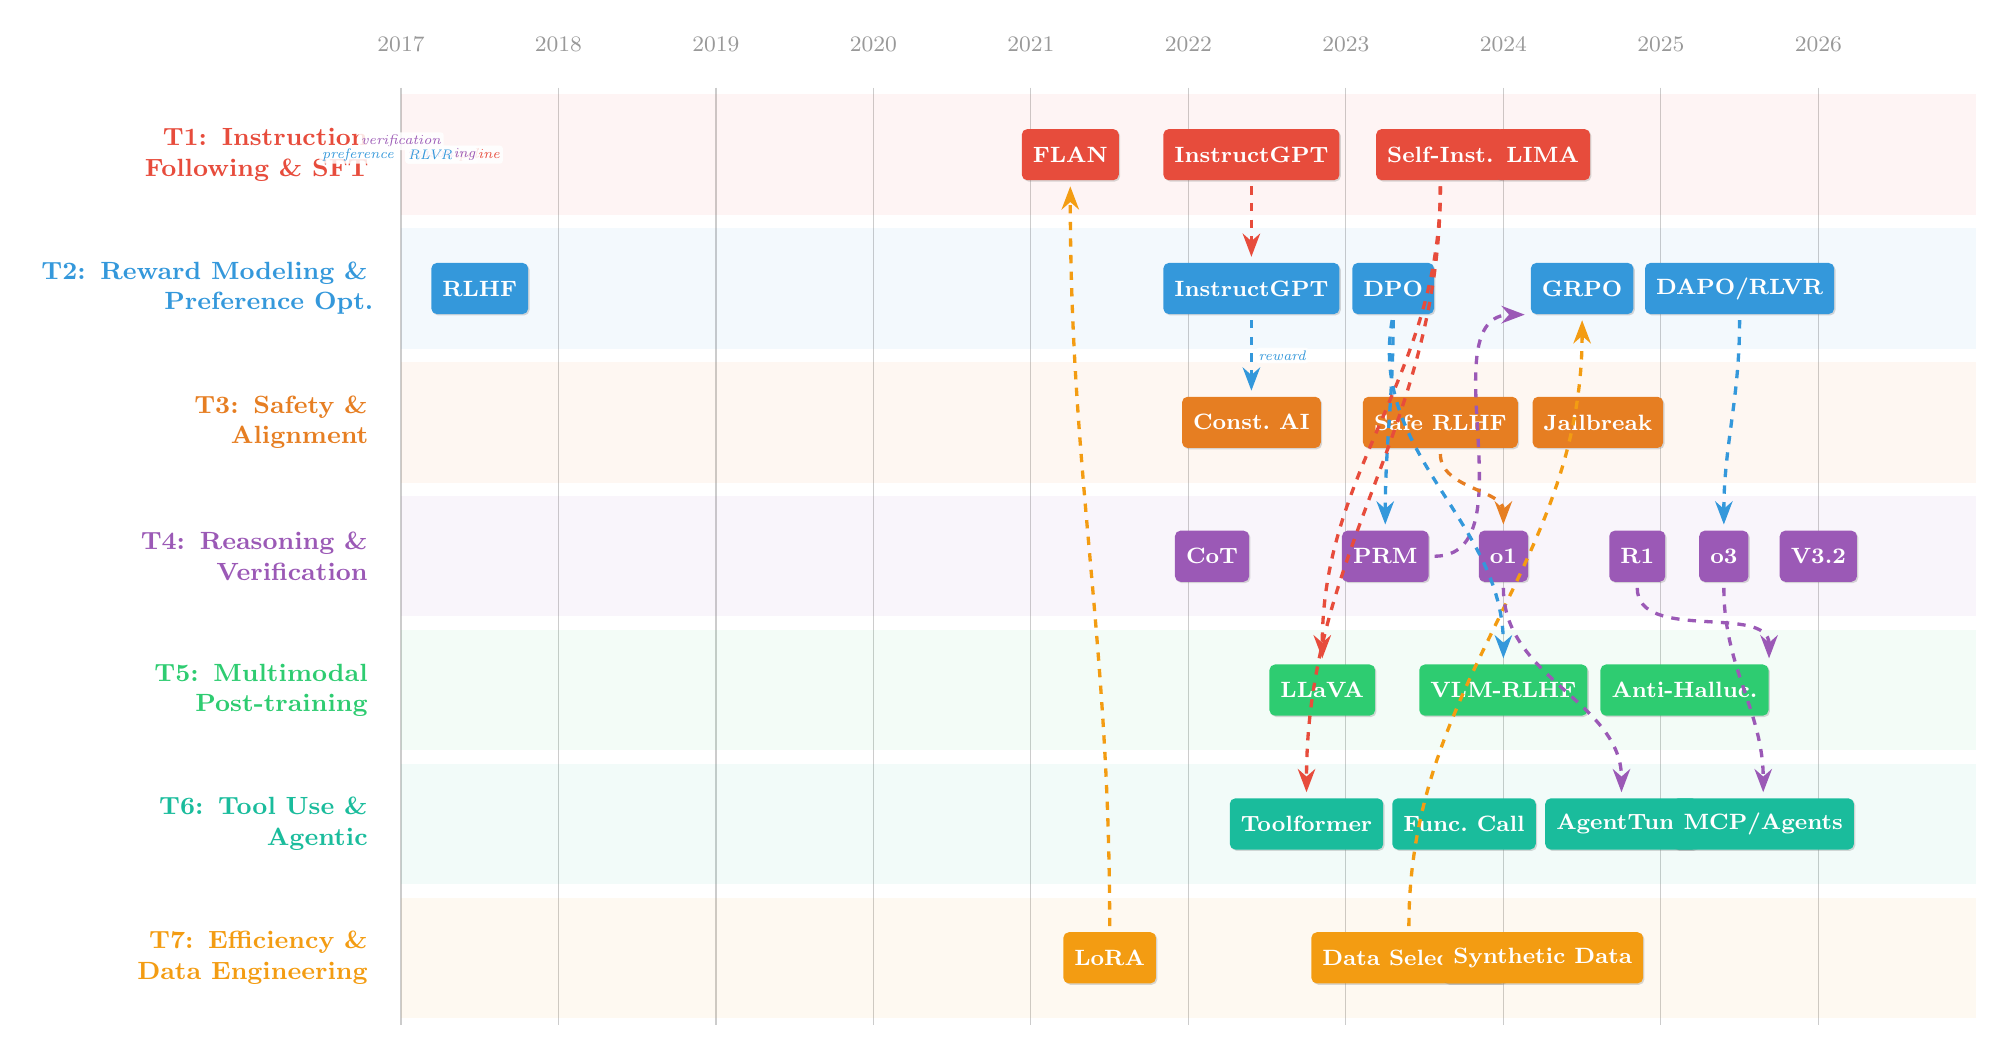
\begin{tikzpicture}[
    >=Stealth,
    node distance=0.6cm,
    paper/.style={
        rounded corners=2pt,
        font=\footnotesize\bfseries,
        inner sep=4pt,
        minimum height=0.65cm,
        text=white,
        drop shadow={shadow xshift=0.5pt, shadow yshift=-0.5pt, opacity=0.3},
    },
    crossarrow/.style={
        ->,
        dashed,
        very thick,
        shorten >=2pt,
        shorten <=2pt,
    },
    arrowlabel/.style={
        font=\tiny\itshape,
        fill=white,
        fill opacity=0.85,
        text opacity=1,
        inner sep=1pt,
        rounded corners=1pt,
    },
    lanelabel/.style={
        font=\small\bfseries,
        anchor=east,
        text width=4.2cm,
        align=right,
    },
]

% --- Geometry ---
\def\laneheight{1.7}   % vertical spacing between lanes
\def\xmin{0}
\def\xmax{20}          % total width
% Year mapping: 2017 = 0, 2026 = 20  =>  1 year = 2 units
\newcommand{\yearx}[1]{\fpeval{(#1-2017)*2}}

% --- Year axis ---
\foreach \y in {2017,2018,2019,2020,2021,2022,2023,2024,2025,2026} {
    \draw[gray!40] (\yearx{\y}, 0.5*\laneheight) -- (\yearx{\y}, -6.5*\laneheight);
    \node[font=\footnotesize, gray!80, anchor=south] at (\yearx{\y}, 0.7*\laneheight) {\y};
}

% --- Lane backgrounds ---
\foreach \i/\col in {0/thread1,1/thread2,2/thread3,3/thread4,4/thread5,5/thread6,6/thread7} {
    \fill[\col, opacity=0.06]
        (\xmin, -\i*\laneheight+0.45*\laneheight)
        rectangle
        (\xmax, -\i*\laneheight-0.45*\laneheight);
}

% =====================================================================
% Thread 1: Instruction Following & SFT (lane y=0)
% =====================================================================
\def\laneA{0}
\node[lanelabel, text=thread1] at (-0.3, \laneA*\laneheight)
    {T1: Instruction\\Following \& SFT};

\node[paper, fill=thread1] (flan)
    at (\yearx{2021}+0.5, \laneA*\laneheight) {FLAN};
\node[paper, fill=thread1] (instructgpt-sft)
    at (\yearx{2022}+0.8, \laneA*\laneheight) {InstructGPT};
\node[paper, fill=thread1] (selfinstruct)
    at (\yearx{2023}+1.2, \laneA*\laneheight) {Self-Inst.};
\node[paper, fill=thread1] (lima)
    at (\yearx{2024}+0.5, \laneA*\laneheight) {LIMA};

% =====================================================================
% Thread 2: Reward Modeling & Preference Optimization (lane y=-1)
% =====================================================================
\def\laneB{-1}
\node[lanelabel, text=thread2] at (-0.3, \laneB*\laneheight)
    {T2: Reward Modeling \&\\Preference Opt.};

\node[paper, fill=thread2] (rlhf-og)
    at (\yearx{2017}+1.0, \laneB*\laneheight) {RLHF};
\node[paper, fill=thread2] (instructgpt-rlhf)
    at (\yearx{2022}+0.8, \laneB*\laneheight) {InstructGPT};
\node[paper, fill=thread2] (dpo)
    at (\yearx{2023}+0.6, \laneB*\laneheight) {DPO};
\node[paper, fill=thread2] (grpo)
    at (\yearx{2024}+1.0, \laneB*\laneheight) {GRPO};
\node[paper, fill=thread2] (dapo)
    at (\yearx{2025}+1.0, \laneB*\laneheight) {DAPO/RLVR};

% =====================================================================
% Thread 3: Safety & Alignment (lane y=-2)
% =====================================================================
\def\laneC{-2}
\node[lanelabel, text=thread3] at (-0.3, \laneC*\laneheight)
    {T3: Safety \&\\Alignment};

\node[paper, fill=thread3] (cai)
    at (\yearx{2022}+0.8, \laneC*\laneheight) {Const.\ AI};
\node[paper, fill=thread3] (saferlhf)
    at (\yearx{2023}+1.2, \laneC*\laneheight) {Safe RLHF};
\node[paper, fill=thread3] (jailbreak)
    at (\yearx{2024}+1.2, \laneC*\laneheight) {Jailbreak};

% =====================================================================
% Thread 4: Reasoning & Verification (lane y=-3)
% =====================================================================
\def\laneD{-3}
\node[lanelabel, text=thread4] at (-0.3, \laneD*\laneheight)
    {T4: Reasoning \&\\Verification};

\node[paper, fill=thread4] (cot)
    at (\yearx{2022}+0.3, \laneD*\laneheight) {CoT};
\node[paper, fill=thread4] (prm)
    at (\yearx{2023}+0.5, \laneD*\laneheight) {PRM};
\node[paper, fill=thread4] (oone)
    at (\yearx{2024}+0.0, \laneD*\laneheight) {o1};
\node[paper, fill=thread4] (deepseekr1)
    at (\yearx{2025}-0.3, \laneD*\laneheight) {R1};
\node[paper, fill=thread4] (othree)
    at (\yearx{2025}+0.8, \laneD*\laneheight) {o3};
\node[paper, fill=thread4] (v32)
    at (\yearx{2026}+0.0, \laneD*\laneheight) {V3.2};

% =====================================================================
% Thread 5: Multimodal Post-training (lane y=-4)
% =====================================================================
\def\laneE{-4}
\node[lanelabel, text=thread5] at (-0.3, \laneE*\laneheight)
    {T5: Multimodal\\Post-training};

\node[paper, fill=thread5] (llava)
    at (\yearx{2023}-0.3, \laneE*\laneheight) {LLaVA};
\node[paper, fill=thread5] (vlmrlhf)
    at (\yearx{2024}+0.0, \laneE*\laneheight) {VLM-RLHF};
\node[paper, fill=thread5] (halluc)
    at (\yearx{2025}+0.3, \laneE*\laneheight) {Anti-Halluc.};

% =====================================================================
% Thread 6: Tool Use & Agentic (lane y=-5)
% =====================================================================
\def\laneF{-5}
\node[lanelabel, text=thread6] at (-0.3, \laneF*\laneheight)
    {T6: Tool Use \&\\Agentic};

\node[paper, fill=thread6] (toolformer)
    at (\yearx{2022}+1.5, \laneF*\laneheight) {Toolformer};
\node[paper, fill=thread6] (funccall)
    at (\yearx{2023}+1.5, \laneF*\laneheight) {Func.\ Call};
\node[paper, fill=thread6] (agenttune)
    at (\yearx{2024}+1.5, \laneF*\laneheight) {AgentTune};
\node[paper, fill=thread6] (mcp)
    at (\yearx{2025}+1.3, \laneF*\laneheight) {MCP/Agents};

% =====================================================================
% Thread 7: Efficiency & Data Engineering (lane y=-6)
% =====================================================================
\def\laneG{-6}
\node[lanelabel, text=thread7] at (-0.3, \laneG*\laneheight)
    {T7: Efficiency \&\\Data Engineering};

\node[paper, fill=thread7] (lora)
    at (\yearx{2021}+1.0, \laneG*\laneheight) {LoRA};
\node[paper, fill=thread7] (datasel)
    at (\yearx{2023}+0.8, \laneG*\laneheight) {Data Selection};
\node[paper, fill=thread7] (synthdata)
    at (\yearx{2024}+0.5, \laneG*\laneheight) {Synthetic Data};

% =====================================================================
% Cross-thread arrows (dashed, idea flow)
% =====================================================================

% T1 -> T2: InstructGPT-SFT feeds into InstructGPT-RLHF
\draw[crossarrow, thread1] (instructgpt-sft.south) -- (instructgpt-rlhf.north);

% T2 -> T3: RLHF ideas feed into Constitutional AI
\draw[crossarrow, thread2] (instructgpt-rlhf.south) -- (cai.north)
    node[arrowlabel, midway, right=1pt] {reward};

% T2 -> T4: Reward modeling feeds reasoning verification (PRM)
\draw[crossarrow, thread2] (dpo.south)
    to[out=-90, in=90] (prm.north);

% T4 -> T2: Reasoning verification inspires GRPO
\draw[crossarrow, thread4] (prm.east)
    to[out=0, in=180] (grpo.south west)
    node[arrowlabel, midway, above=1pt] {verification};

% T1 -> T5: SFT pipeline adopted by LLaVA
\draw[crossarrow, thread1] (selfinstruct.south)
    to[out=-90, in=90] (llava.north)
    node[arrowlabel, near start, right=1pt] {SFT pipeline};

% T2 -> T5: RLHF adopted for VLM alignment
\draw[crossarrow, thread2] (dpo.south)
    to[out=-100, in=90] (vlmrlhf.north)
    node[arrowlabel, near end, left=1pt] {preference};

% T1 -> T6: Instruction tuning enables tool use
\draw[crossarrow, thread1] (selfinstruct.south)
    to[out=-90, in=90] (toolformer.north);

% T7 -> T1: LoRA enables efficient SFT
\draw[crossarrow, thread7] (lora.north)
    to[out=90, in=-90] (flan.south)
    node[arrowlabel, near start, right=1pt] {LoRA};

% T7 -> T2: Efficient training enables broader RLHF
\draw[crossarrow, thread7] (datasel.north)
    to[out=90, in=-90] (grpo.south);

% T3 -> T4: Safety constraints shape reasoning alignment
\draw[crossarrow, thread3] (saferlhf.south)
    to[out=-90, in=90] (oone.north)
    node[arrowlabel, midway, right=1pt] {safety};

% T4 -> T6: Reasoning enables agent planning
\draw[crossarrow, thread4] (oone.south)
    to[out=-90, in=90] (agenttune.north)
    node[arrowlabel, midway, right=1pt] {reasoning};

% T2 -> T4: RLVR (DAPO) feeds reasoning training
\draw[crossarrow, thread2] (dapo.south)
    to[out=-90, in=90] (othree.north)
    node[arrowlabel, near start, right=1pt] {RLVR};

% T4 -> T5: Reasoning RL migrates to multimodal (R1-VL, MM-Eureka)
\draw[crossarrow, thread4] (deepseekr1.south)
    to[out=-90, in=90] (halluc.north east);

% T4 -> T6: Thinking models empower agent planning
\draw[crossarrow, thread4] (othree.south)
    to[out=-90, in=90] (mcp.north);

\end{tikzpicture}%
}% end resizebox
\caption{Post-training 领域的 Hybrid Problem-Evolution Graph 全景视图。
七条水平泳道分别对应七条演化线程，
x 轴为时间线（2017--2026），
节点为各线程内的 landmark 工作，
虚线箭头表示跨线程的思想流动与技术迁移。}
\label{fig:overview}
\end{figure}


\noindent
在接下来的章节中，我们将沿着每条线程深入分析 landmark 论文的技术细节，
同时通过跨线程引用保持全局视角。读者可以按照线程顺序（T1--T7）线性阅读，
也可以从任意感兴趣的线程入手，通过交叉引用跳转到相关线程。


% === Thread 1: Instruction Following & SFT ===
% === Thread 1: Instruction Following & SFT ===
\section{Thread 1: Instruction Following \& SFT}
\label{sec:sft}

\begin{quote}
\textit{Core Question: 如何让 pre-trained language model 学会理解并遵循人类指令？}
\end{quote}

Instruction following 是 post-training 最早且最基本的目标。
一个仅经过 pre-training 的 language model 本质上是一个 next-token predictor：
给定 prompt ``What is the capital of France?''，它可能续写 ``What is the capital of Germany?''，
而非回答 ``Paris''。
Supervised Fine-Tuning（SFT）通过在 (instruction, response) 数据对上进行有监督训练，
教会模型理解指令意图并生成符合预期格式的输出。

本章追踪 SFT 领域从问题提出到当前 open problems 的完整演化链条。
我们将看到该领域如何沿着两条核心轴线演进：
\textbf{数据维度}（从人工标注到合成生成，从追求数量到重视质量）
和\textbf{任务维度}（从单一任务到 multi-task scaling，从通用能力到 domain-specific specialization）。

\evolution{Pre-trained LM 只会续写，不会回答}{Instruction-tuned LM 理解指令意图}{SFT on (instruction, response) pairs}


% ========================================================
\subsection{问题起源：为什么预训练模型不够？}
\label{sec:sft:origin}

Pre-training 的目标函数——无论是 autoregressive language modeling 还是 masked language modeling——
与用户的实际使用方式之间存在根本性的 misalignment。
这一问题可以从三个层面理解：

\begin{problembox}
\begin{enumerate}[leftmargin=1.5em]
  \item \textbf{目标函数 mismatch}：
    Pre-training 优化的是 $\mathcal{L}_{\text{PT}} = -\sum_t \log P(x_t \mid x_{<t})$，
    即对 training corpus 中所有 token 的预测概率取对数似然。
    这一目标对所有 token 一视同仁，不区分指令理解、知识回忆和格式遵循。
    但用户需要的是：给定一个 instruction $x$，模型应生成一个 helpful、accurate 且 safe 的 response $y$。

  \item \textbf{行为模式 mismatch}：
    Pre-trained model 学到的是 web-scale corpus 中最常见的文本分布。
    这意味着它会模仿训练数据中的各种风格——新闻报道、社交媒体帖子、代码注释——
    而非专注于作为 AI assistant 的对话模式。
    换言之，pre-trained model 知道很多东西，但不知道如何以一个 assistant 的身份表达。

  \item \textbf{格式 mismatch}：
    Pre-trained model 缺乏对输出格式的认知。
    当用户要求 ``List 5 benefits of exercise''，模型可能生成一篇散文而非编号列表；
    当用户提问 ``Is X true?''，模型可能继续生成更多问题而非给出回答。
\end{enumerate}
\end{problembox}

\noindent
Instruction tuning 的核心思想是通过少量但高质量的 (instruction, response) 数据
对模型进行 supervised fine-tuning，使其学会：
(1) 从 instruction 中提取用户意图，
(2) 调用 pre-training 阶段习得的知识来回应，
(3) 以符合预期的格式和风格组织输出。

\begin{solutionbox}
给定 instruction-response 数据集 $\mathcal{D} = \{(x_i, y_i)\}_{i=1}^N$，
SFT 的训练目标为：
\[
  \mathcal{L}_{\text{SFT}} = -\sum_{i=1}^{N} \sum_{t=1}^{|y_i|}
    \log P_\theta(y_{i,t} \mid x_i, y_{i,<t})
\]
注意 loss 只在 response tokens $y$ 上计算（instruction tokens $x$ 被 mask），
这确保模型学习的是"如何回应指令"而非"如何生成指令"。
\end{solutionbox}


值得注意的是，instruction tuning 并非适配 pre-trained LM 的唯一路径。
Prompt tuning \citep{lester2021prompt} 和 Prefix-Tuning \citep{li2021prefix}
采用了另一种思路——冻结模型参数，仅优化输入端的连续 prompt embedding。
这类 parameter-efficient 方法在特定任务上表现优异，
但难以赋予模型通用的 instruction following 能力。
FLAN 的后续实验（Fig.~10）甚至表明，instruction tuning 可以\emph{促进}
后续的 prompt tuning 效果，暗示两者并非竞争关系而是互补关系。

% ========================================================
\subsection{奠基方法：早期探索与范式确立}
\label{sec:sft:foundation}

2021--2022 年间，三项独立且几乎同时的工作从不同角度证明了
instruction tuning 的有效性，奠定了该领域的基础范式。


% --- FLAN ---
\subsubsection{FLAN: Instruction Tuning for Zero-Shot Generalization}
\label{sec:sft:flan}

\landmark{wei2022flan}
FLAN（Finetuned Language Net）是最早系统性地验证
instruction tuning 可以提升模型 zero-shot 泛化能力的工作之一。

\paragraph{核心设计。}
FLAN 的实验基于 LaMDA-PT（137B 参数的 decoder-only Transformer），
使用 62 个 NLP 数据集，按任务类型组织为 10 个 cluster
（如 Natural Language Inference, Sentiment Analysis, Reading Comprehension 等）。
对于每个数据集，作者手工编写 10 个 instruction template，将传统 NLP 样本转化为
自然语言指令格式。
例如，一个 NLI 样本 (\texttt{premise}, \texttt{hypothesis}, \texttt{label})
被转化为 ``Premise: [P]. Hypothesis: [H]. Does the premise entail the hypothesis?''。

\paragraph{关键实验发现。}
FLAN 的实验设计极为精巧——在评估某个 cluster 的 zero-shot 性能时，
训练数据中\textbf{排除}该 cluster 的所有任务，确保评测的是真正的跨任务泛化能力：

\begin{enumerate}[leftmargin=1.5em]
  \item \textbf{Zero-shot FLAN 超越 zero-shot GPT-3}：
    在 25 个评测任务中的大多数上，FLAN 的 zero-shot 性能优于 GPT-3 的 zero-shot 性能，
    甚至在部分任务上接近或超越 GPT-3 的 few-shot 性能。

  \item \textbf{Task cluster 数量的 scaling 效应}：
    随着训练中包含的 task cluster 数量从 1 增加到 7，
    held-out cluster 上的平均性能从 49.9\% 持续提升至 63.5\%，
    呈现近乎线性的增长趋势。
    这证明了 instruction tuning 的泛化能力随任务多样性单调递增。

  \item \textbf{模型规模的阈值效应}：
    Instruction tuning 对大模型（$\geq$ 100B 参数）有显著提升，
    但对小模型（$\leq$ 8B 参数）反而可能造成性能下降。
    作者推测这是因为小模型的容量不足以同时学习多个任务的 instruction following，
    导致 catastrophic forgetting。

  \item \textbf{Instruction 的关键作用}：
    消融实验表明，使用自然语言 instruction 模板（55.2\%）
    与不使用 instruction 的 baseline（37.3\%）之间存在近 18 个百分点的巨大差距，
    证明 instruction 本身——而非仅仅是多任务训练——是泛化能力提升的关键。
\end{enumerate}

\paragraph{FLAN 的意义与局限。}
FLAN 确立了 instruction tuning 的基本范式：
通过在多个任务的 instruction 格式数据上训练，模型可以泛化到未见过的任务。
但 FLAN 也存在明显局限：
(1) 所有 instruction template 均为人工编写，扩展成本高；
(2) 任务类型受限于传统 NLP benchmark，缺乏开放域对话和创意生成等真实用户场景；
(3) 仅在 137B 规模验证，对较小模型的适用性存疑。


% --- T0 ---
\subsubsection{T0: Prompted Training for Zero-Shot Generalization}
\label{sec:sft:t0}

\landmark{sanh2022multitask}
T0 与 FLAN 几乎同时发表，独立地验证了相似的核心思想，
但在实验设计和模型选择上有所不同。

T0 基于 encoder-decoder 架构的 T5（11B 参数），
使用 Public Pool of Prompts (P3) 数据集——
涵盖 62 个数据集的 2,073 个人工编写的 prompt template。
在 11 个 held-out 任务上，T0 的 zero-shot 性能
在 7 个任务上匹配或超越了 GPT-3 的 few-shot（16-shot）性能，
尽管 T0 的参数量仅为 GPT-3 的 $1/16$。

T0 与 FLAN 的互补性体现在：
(1) T0 证明了 encoder-decoder 架构同样受益于 instruction tuning，不限于 decoder-only；
(2) P3 的大规模 prompt template 库为后续研究提供了宝贵的数据资源；
(3) T0 的 prompt engineering 实践积累了关于 template 设计对性能影响的经验知识。

与 FLAN 同时期，\citet{mishra2021crossfit} 提出了利用 crowdsourcing 方式
收集 cross-task instruction 数据的方法，
\citet{wang2022supernaturalinstructions} 则将这一思路扩展为
Super-NaturalInstructions——一个包含 1,616 个任务的大规模 benchmark，
为后续的 multi-task instruction tuning 提供了重要的数据基础设施。


% --- InstructGPT ---
\subsubsection{InstructGPT: 确立三阶段训练范式}
\label{sec:sft:instructgpt}

\landmark{ouyang2022instructgpt}
如果说 FLAN 和 T0 证明了 instruction tuning 在学术 benchmark 上的有效性，
InstructGPT 则将其推向了真实用户场景，
并确立了影响深远的 ``SFT $\rightarrow$ Reward Model $\rightarrow$ PPO'' 三阶段训练范式。

\paragraph{SFT 阶段的技术细节。}
InstructGPT 的 SFT 阶段使用约 13,000 条由人类标注者撰写的 demonstration 数据。
这些数据来自两个来源：
(1) OpenAI API 收集的真实用户 prompt（经过筛选和脱敏），
(2) 标注者根据 task distribution 主动编写的 prompt。
训练配置：16 epochs，cosine learning rate decay，残差连接上的 dropout（$p=0.2$）。
作者发现在小数据集上多 epoch 训练是有效的——尽管训练数据量远小于 pre-training 语料，
但 SFT 仍能显著改变模型的行为模式。

\paragraph{核心发现。}
InstructGPT 最震撼的结论是：
\textbf{1.3B 参数的 SFT+RLHF 模型在人类评估中以 85$\pm$3\% 的胜率超越了 175B 参数的原始 GPT-3}。
这意味着 post-training 可以在不增加模型规模的前提下实现质的飞跃——
参数量相差 100 倍以上，但经过 alignment 的小模型更受用户青睐。
此外，InstructGPT 在 truthfulness 上的表现约为 GPT-3 的两倍（TruthfulQA），
hallucination 率从 41\% 降至 21\%。

\paragraph{Alignment Tax。}
InstructGPT 首次系统性地识别了 \textbf{alignment tax}——
即 post-training 在提升 instruction following 和安全性的同时，
可能导致模型在传统 NLP benchmark 上的性能下降。
作者通过在 PPO 目标中加入 pre-training 数据的混合训练（PPO-ptx）来缓解这一问题：
\[
  \text{objective}(\theta) =
    \mathbb{E}_{(x,y) \sim \pi_{\text{RL}}} \big[ r_\theta(x,y) - \beta \log \frac{\pi_{\text{RL}}(y|x)}{\pi_{\text{SFT}}(y|x)} \big]
    + \gamma \, \mathbb{E}_{x \sim \mathcal{D}_{\text{pretrain}}} \big[ \log \pi_{\text{RL}}(x) \big]
\]
其中第二项通过保持模型在 pre-training 分布上的性能来减轻 alignment tax。
\crossref{2}{sec:pref}

\paragraph{InstructGPT 对后续研究的影响。}
InstructGPT 的影响远超其技术贡献本身。
它确立了两个持续至今的 paradigm：
(1) SFT 作为 RLHF/DPO pipeline 的必要前置阶段
（几乎所有后续的 preference optimization 工作都从一个 SFT checkpoint 开始）；
(2) 人类评估（human evaluation）作为 instruction-following 模型的金标准评测方式
（而非仅依赖 automatic metrics）。


% ========================================================
\subsection{局限与分支：数据挑战与解决路径的分化}
\label{sec:sft:branching}

FLAN、T0 和 InstructGPT 确立了 instruction tuning 的有效性，
但也暴露了一个核心瓶颈：\textbf{高质量 instruction 数据的获取成本极高}。
InstructGPT 的 13,000 条 demonstration 数据由 40 名专业标注者花费数月完成，
这对学术界和开源社区而言是不可承受的成本。

\begin{problembox}
如何以低成本获取大规模、高质量的 instruction tuning 数据？
\end{problembox}

这一问题催生了两条几乎相反的解决路径：
\textbf{Branch A} 追求数据数量的扩展（通过合成生成降低成本），
\textbf{Branch B} 追求数据质量的提纯（通过精心筛选以少胜多）。
两者之间的张力构成了 SFT 领域最核心的 debate。

\evolution{人工标注数据成本高昂}{Branch A: 合成数据 / Branch B: 数据精选}{降低 instruction data 获取门槛}


% --- Branch A: Synthetic Data ---
\subsubsection{Branch A: 合成数据生成——以量取胜}
\label{sec:sft:synthetic}

利用 language model 自身生成训练数据的思想可以追溯到
\citet{schick2021generating}，他们证明 GPT-2 级别的模型
即可为 SuperGLUE 任务生成有效的标注数据，
且在部分任务上生成数据训练的模型性能接近人工标注数据。
这一结果预示了 ``LM 既是学生也是老师'' 的可能性。

\paragraph{Self-Instruct: 从 LM 自身 bootstrap 指令数据。}
\landmark{wang2023selfinstruct}
Self-Instruct 将这一思路从特定任务的标注数据扩展到\textbf{通用 instruction 数据}的生成，
成为 synthetic instruction data 领域最具影响力的工作。
它开创了利用模型自身能力来生成训练数据的 bootstrap 范式。

\textbf{Pipeline 设计。}
Self-Instruct 的 pipeline 包含四个阶段：
\begin{enumerate}[leftmargin=1.5em]
  \item \textbf{Instruction 生成}：
    从 175 个人工编写的 seed task 出发，通过 in-context learning 让
    vanilla GPT-3（text-davinci-001）生成新的 instruction。
    每轮从 task pool 中采样 6 个人工 seed + 2 个模型生成的 instruction 作为 few-shot example。

  \item \textbf{分类识别}：
    判断每个 instruction 是 classification task 还是 non-classification task，
    因为两者需要不同的 instance 生成策略。

  \item \textbf{Instance 生成}：
    对 non-classification task 采用 input-first approach（先生成 input 再生成 output），
    对 classification task 采用 output-first approach（先确定 label 再生成 input），
    后者可以有效避免 label 分布的偏斜。

  \item \textbf{过滤}：
    使用 ROUGE-L $< 0.7$ 的阈值过滤与已有数据过于相似的新生成样本，
    确保数据多样性。
\end{enumerate}

\textbf{结果。}
从 175 个 seed task 出发，Self-Instruct 生成了 52,445 条 instruction 和 82,439 个 instance。
质量评估显示：92\% 的生成 instruction 是有效的，54\% 的样本在所有字段上均有效。
在 SuperNI benchmark 上，使用 Self-Instruct 数据微调的 GPT-3
比 vanilla GPT-3 高出 33.1\% ROUGE-L，
人类评估中仅落后 InstructGPT$_{\text{001}}$ 约 5\%。
整个数据生成过程的 API 成本仅约 \$600。

\textbf{意义。}
Self-Instruct 的意义在于证明了 \textbf{LM 自身可以作为 instruction data 的来源}，
这一思想直接催生了一系列后续工作。

\paragraph{Alpaca: 将 Self-Instruct 工业化。}
Stanford Alpaca \citep{taori2023alpaca} 将 Self-Instruct 的思路应用于 LLaMA 7B，
使用 GPT-3.5（text-davinci-003）生成 52K 条 instruction 数据，
微调成本仅约 \$600（API）+ \$100（训练）。
Alpaca 在 human evaluation 中展现了与 GPT-3.5 相当的性能，
成为开源 instruction-following 模型的里程碑。
但 Alpaca 也暴露了 synthetic data 的局限：
生成数据中存在显著的 hallucination 和 style mimicry（模仿 teacher model 的语言风格
而非真正学习底层能力），引发了对 synthetic data ceiling 的讨论。
与此同时，Vicuna \citep{chiang2023vicuna} 提供了一条对比路径：
它使用 ShareGPT 平台收集的约 70K 条\textbf{真实用户与 ChatGPT 的对话}
对 LLaMA 13B 进行微调，在 GPT-4 评估中达到了 ChatGPT 约 90\% 的质量。
Vicuna 的成功表明，真实对话数据在捕捉用户交互模式方面具有
synthetic data 难以替代的优势——用户的提问方式、多轮对话的上下文依赖、
以及 implicit preference 都蕴含在真实交互中。
Alpaca（synthetic data）与 Vicuna（real conversation data）
的并行发展，为后续关于数据来源选择的讨论奠定了实证基础。

\paragraph{WizardLM: Evol-Instruct 渐进式复杂化。}
\citet{xu2024wizardlm} 提出 Evol-Instruct 方法——
不直接从头生成 instruction，而是对已有的简单 instruction 进行迭代进化。
每轮进化通过 prompt 让 LLM 对 instruction 执行以下操作之一：
添加约束条件、增加推理步骤、具体化场景、增加输入复杂度。
经过多轮进化后，简单的 ``Write a poem about spring'' 可能变为
``Write a Shakespearean sonnet about spring, incorporating at least three
metaphors related to scientific phenomena, and ending with a volta
that challenges the reader's expectations''。
这一方法在 instruction 复杂度维度上实现了有控制的数据增强。

\paragraph{其他合成数据工作。}
\citet{honovich2022unnatural} 的 Unnatural Instructions 采用与 Self-Instruct 类似的方法
但使用更少的 seed（15 个），验证了 bootstrap 的鲁棒性。
\citet{peng2023gpt4instruct} 使用 GPT-4 生成更高质量的 instruction 数据，
展示了 teacher model 能力对 synthetic data 质量的决定性影响。
Orca \citep{mukherjee2023orca} 提出了 progressive learning 策略——
从 GPT-4 的 detailed reasoning trace 中学习，
不仅模仿最终答案，更模仿推理过程（system message 中要求 GPT-4 ``explain step by step''），
这一思想预示了 Thread 4 中 reasoning distillation 的发展方向
\crossref{4}{sec:thread4}。
Baize \citep{xu2023baize} 则探索了利用 ChatGPT 自我对话生成多轮对话数据的方法。


% --- Branch B: Data Quality ---
\subsubsection{Branch B: 数据质量精选——以质取胜}
\label{sec:sft:quality}

\paragraph{LIMA: Superficial Alignment Hypothesis。}
\landmark{zhou2023lima}
LIMA 提出了 SFT 领域最具争议性的假说之一——
\textbf{Superficial Alignment Hypothesis}（表层对齐假说）：
\textit{模型的知识和能力几乎全部在 pre-training 阶段习得，
alignment 的作用仅在于教会模型正确的输出格式和交互风格}。

\textbf{实验设计。}
LIMA 仅使用 1,000 条精心筛选的训练样本对 LLaMA 65B 进行微调。
数据来源的多样性经过精心设计：
750 条来自社区问答平台（Stack Exchange 答案中选取回复质量最高的、
wikiHow 文章、Reddit 高赞帖子），
250 条由作者手动编写（确保涵盖特定的对话能力和安全行为）。
训练配置看似简单但经过仔细调优：
15 epochs，AdamW 优化器，residual dropout 从底层的 $p_d = 0.0$ 线性增加到顶层的 $p_d = 0.3$。
这种 \textbf{layer-wise increasing dropout} 是一个值得注意的细节——
它保护了底层（更接近 pre-training 知识）的表示稳定性，
同时允许顶层（更接近输出格式）有更大的学习自由度。

\textbf{核心结果。}
在人类评估中，LIMA 的表现令人惊讶：
\begin{itemize}[leftmargin=1.5em]
  \item 50\% 的输出被评为 ``excellent''，88\% 为 ``pass'' 或更好
  \item 与 Alpaca 65B 对比：53\% 的情况下 LIMA 被偏好
  \item 与 DaVinci003 对比：44\% 的情况下 LIMA 被偏好或持平
  \item 与 GPT-4 对比：43\% 的情况下 LIMA 表现相当或更优
\end{itemize}

\textbf{消融实验}（在 7B 模型上进行）提供了更精细的洞见：
\begin{itemize}[leftmargin=1.5em]
  \item \textbf{多样性 $>$ 同质性}：
    多样化的 Stack Exchange 数据（rating 3.83/6）优于同质化的 wikiHow 数据（3.49/6），
    证明来源多样性比数据量更重要。
  \item \textbf{质量筛选有效}：
    经过人工筛选的数据（3.83/6）显著优于未筛选的数据（3.33/6）。
  \item \textbf{数量 scaling 存在天花板}：
    从 2K 样本增加到 4K 样本后，性能提升趋于饱和。
  \item \textbf{少量对话数据有大作用}：
    仅加入 30 条多轮对话样本，就将 ``excellent'' 评级从 45.2\% 提升至 76.1\%。
\end{itemize}

\textbf{LIMA 的争议。}
LIMA 的 Superficial Alignment Hypothesis 引发了持续的讨论。
支持者认为它揭示了 SFT 的本质——不是教模型新知识，而是激活已有能力的正确表达方式。
批评者则指出：
(1) 1,000 条数据的实验结论能否泛化到更复杂的能力（如 multi-step reasoning、code generation）尚不明确；
(2) LIMA 使用了 65B 参数的 LLaMA——对于更小的模型，SFT 可能确实需要传授新知识而非仅仅调整格式；
(3) LIMA 的评估主要基于单轮开放域问答，对专业领域和长程任务的覆盖不足。

\paragraph{数据选择方法论。}
LIMA 的成功激发了一系列数据选择方法的研究。
\citet{li2023ifd} 提出 Instruction-Following Difficulty (IFD) 指标——
通过比较模型在有/无 instruction 条件下的输出概率差异来衡量每条数据的信息量，
选择 IFD 最高的样本进行训练。
DEITA \citep{liu2024deita} 提出了基于 complexity、quality 和 diversity 三维度的
自动化数据评分框架，使用 ChatGPT 对数据进行评分排序，
然后通过 embedding-based 多样性过滤选择最优子集。
\citet{chen2023maybeonly} 发现仅使用 0.5\% 的 Alpaca 数据即可达到全量训练 90\% 以上的性能。
Instruction Mining \citep{cao2023instructionmining} 则通过训练一个 quality predictor
来自动化数据筛选过程。

\paragraph{开源数据集与社区贡献。}
OpenAssistant Conversations \citep{kopf2023openassistant} 提供了
一个由 13,500 名志愿者贡献的多语言对话数据集（161,443 条消息，35 种语言），
展示了 crowdsourcing 在 instruction data 收集中的潜力。
Dolly \citep{conover2023dolly} 由 Databricks 的 5,000 名员工在工作时间贡献约 15,000 条数据，
是最早的企业级开源 instruction 数据集之一。


% --- Multi-task Scaling ---
\subsubsection{Branch C: Multi-task Scaling——任务数量维度的扩展}
\label{sec:sft:multitask}

\paragraph{Flan-v2: 将 instruction tuning 推向极致。}
\landmark{chung2022flan}
Flan-v2 是 FLAN 的大规模后续工作，
将 instruction tuning 的任务规模推向了前所未有的高度。

\textbf{数据规模。}
Flan-v2 整合了四个主要的 task collection：
Muffin（80 个任务）、T0-SF（193 个任务）、NIV2（1,554 个任务）、以及 CoT（9 个推理任务），
总计 1,836 个任务（473 个 unique 数据集，146 个任务类别）。
这一规模比原始 FLAN 的 62 个任务扩大了约 30 倍。

\textbf{核心发现。}
\begin{enumerate}[leftmargin=1.5em]
  \item \textbf{跨架构有效性}：
    Flan-v2 在 T5（encoder-decoder, 80M--11B）、
    PaLM（decoder-only, 8B--540B）以及 cont-PaLM 和 U-PaLM 上均验证了有效性，
    证明 instruction tuning 的收益与模型架构无关。

  \item \textbf{任务 scaling 的边际效应}：
    性能随任务数量的增加持续提升，但大部分收益集中在前 282 个任务，
    后续任务的边际贡献递减。
    这提示了一个重要的 practical insight：
    达到"足够好"的性能不需要穷尽所有可能的任务。

  \item \textbf{极端的效率优势}：
    以 PaLM 540B 为例，Flan 微调仅使用 512 个 v4 TPU chips 训练 37 小时，
    计算量仅为 pre-training 的 \textbf{0.2\%}。
    但效果显著：Flan-PaLM 540B 在 MMLU 上达到 75.2\%（5-shot, with CoT + self-consistency），
    normalized average 提升 9.4--15.5\%。
    更惊人的是，\textbf{Flan-T5-XL 3B 在 MMLU 上达到 52.4\%，超越了 GPT-3 175B 的 43.9\%}——
    一个 $1/58$ 参数量的模型在 instruction tuning 后超越了 $58\times$ 大的模型。

  \item \textbf{CoT 微调的关键作用}：
    Flan-v2 中一个被低估但极其重要的发现是关于 Chain-of-Thought 微调的。
    不包含 CoT 数据的 instruction tuning 会\textbf{损害}模型的推理能力；
    但将 CoT 数据与 non-CoT 数据联合训练，
    不仅保持了推理能力，还同时提升了两类任务的性能。
    此外，CoT 微调 unlocked 了 zero-shot CoT 能力——
    仅通过在 prompt 末尾添加 ``Let's think step by step''
    就能激发模型的推理行为，无需提供 few-shot reasoning example。
    这一发现预示了 Thread 4 中 reasoning post-training 的发展方向
    \crossref{4}{sec:thread4}。
\end{enumerate}

Flan Collection \citep{longpre2023flancollection} 随后开源了 Flan-v2 的完整数据混合方案和模板，
为社区提供了可复现的基础。
OPT-IML \citep{iyer2022optiml} 在 Meta 的 OPT 模型上复现了类似的 multi-task instruction tuning 实验。
BLOOMZ/mT0 \citep{muennighoff2022bloomz} 将 multi-task instruction tuning
扩展到多语言场景（crosslingual instruction tuning with xP3 dataset），
证明了该范式在非英语语言上的有效性。


% --- Domain-specific SFT ---
\subsubsection{Branch D: Domain-Specific SFT——专业领域的精准适配}
\label{sec:sft:domain}

随着通用 instruction tuning 趋于成熟，研究者开始将 SFT 技术应用于
需要专业知识的垂直领域，催生了 domain-specific SFT 的研究热潮。

\paragraph{Code: 数据质量可以打破 scaling law。}
\landmark{gunasekar2023phi1}
phi-1 是 code SFT 领域最具颠覆性的工作。
这项来自 Microsoft Research 的研究使用仅 1.3B 参数的模型，
在 HumanEval 上达到 50.6\% pass@1，在 MBPP 上达到 55.5\% pass@1——
在当时超越了许多参数量大一个数量级的模型。

\textbf{核心创新在于数据工程。}
phi-1 的训练数据包含三个精心设计的组成部分：
\begin{itemize}[leftmargin=1.5em]
  \item \textbf{Filtered code-language corpus}（约 6B tokens）：
    从 The Stack 和 StackOverflow 中使用随机森林分类器筛选
    ``textbook quality'' 的代码片段。
    分类器训练在 GPT-4 标注的少量样本上（对每个代码片段标注其 educational value），
    然后用于对整个语料库进行大规模筛选。

  \item \textbf{Synthetic textbooks}（$< 1$B tokens）：
    使用 GPT-3.5 生成类似教科书风格的 Python 教学内容，
    包含概念解释、代码示例和循序渐进的练习。

  \item \textbf{CodeExercises}（$< 180$M tokens）：
    使用 GPT-3.5 生成函数级别的编程练习（function docstring + solution），
    作为 fine-tuning 阶段的训练数据。
\end{itemize}

\textbf{关键洞见。}
phi-1 的成功挑战了传统的 scaling law 思维——
它证明 \textbf{数据质量可以在一定程度上替代模型规模和数据量}。
一个 10$\times$ 小的模型在 100$\times$ 少的数据上训练，
可以匹配甚至超越大模型的性能。
更有趣的是，phi-1 在 fine-tuning 后展现出一些\textbf{emergent capabilities}——
包括使用 Pygame、Tkinter 等外部库的能力以及 chat-style 的交互模式——
这些能力并未在 fine-tuning 数据中出现过，暗示高质量数据可能有助于模型
更好地组织和泛化 pre-training 阶段习得的知识。
这一发现与 LIMA 的 Superficial Alignment Hypothesis 形成了有趣的呼应。

WizardCoder \citep{luo2023wizardcoder} 将 WizardLM 的 Evol-Instruct 方法应用于代码领域，
通过对编程 instruction 进行渐进式复杂化来生成高难度训练数据。
Magicoder \citep{wei2023magicoder} 提出 OSS-Instruct——
从真实的开源代码片段出发，让 LLM 为这些代码生成对应的 instruction，
确保训练数据的代码风格和复杂度与真实项目一致。

\paragraph{Math: 推理增强的 SFT。}
数学推理是 domain-specific SFT 的另一个活跃方向。
WizardMath \citep{luo2023wizardmath} 将 Evol-Instruct 扩展到数学领域，
结合 Reinforced Evol-Instruct 进一步提升数据质量。
MAmmoTH \citep{yue2023mammoth} 构建了混合 CoT 和 Program-of-Thought（PoT）的
instruction 数据集——对适合符号计算的问题使用 Python 代码作为推理步骤，
对需要语义理解的问题使用自然语言 CoT。
MetaMath \citep{yu2023metamath} 提出对数学问题进行 question bootstrapping——
通过改写问题的表述方式（同义替换、条件反转、自问自答分解）来增强数据多样性，
同时保持数学内容的正确性。
RFT \citep{yuan2023rft}（Rejection sampling Fine-Tuning）
研究了在数学推理中的 sampling-then-filtering 策略：
对每个数学问题让模型生成多个候选答案，仅保留最终答案正确的样本用于 SFT，
并分析了 sampling 数量与最终性能之间的 scaling relationship。

\paragraph{Multilingual \& Other Domains.}
Aya Model \citep{ustun2024aya} 是 multilingual instruction tuning 的重要里程碑，
覆盖 101 种语言，展示了 instruction tuning 在极端多语言场景下的可行性和挑战。
Gorilla \citep{patil2023gorilla} 专注于 API 调用能力，
通过在 API 文档和调用示例上进行 SFT，使模型能准确生成复杂的 API 调用代码
\crossref{6}{sec:thread6}。
Platypus \citep{lee2023platypus} 针对 STEM 领域进行了小规模精选 SFT。
LongForm \citep{koksal2023longform} 则聚焦于长文本生成任务的 instruction tuning。


% ========================================================
\subsection{收敛与前沿：系统性综合与方法论融合}
\label{sec:sft:convergence}

2023 年下半年，SFT 领域从百花齐放的探索期进入系统性综合的阶段。
多个工作开始整合前述 branch 的经验，试图回答：
\textbf{如何将数据工程、multi-task training 和 domain specialization
融合为一个统一的最佳实践？}

\evolution{Branch A (合成) / Branch B (精选) / Branch C (scaling) 各自发展}%
  {系统性综合: 融合多条路径的最佳实践}{实验驱动的 recipe 研究}


% --- Tulu ---
\subsubsection{Tulu: 开源 SFT Recipe 的系统性探索}
\label{sec:sft:tulu}

Tulu \citep{wang2023tulu} 是第一个系统性地比较不同 instruction data
sources 和 training strategies 的开源工作。
通过在 LLaMA 上控制变量实验，Tulu 回答了多个实践性问题：
哪些数据源的组合最有效？数据混合比例如何影响性能？
Human-written 和 synthetic data 在不同任务上的相对优势如何？

Tulu 2 \citep{ivison2023tulu2} 进一步扩展了这一研究，
将实验范围从 SFT 扩展到完整的 post-training pipeline（SFT + DPO），
并在 LLaMA 2 系列模型上验证了最优 recipe。
Tulu 2 的核心贡献在于提供了一个 reproducible 的 training recipe——
包括数据混合策略、超参数配置和评估 protocol——
使开源社区可以在此基础上迭代优化。

\subsubsection{Zephyr \& OpenChat: 从强模型到弱模型的知识蒸馏}
\label{sec:sft:distillation}

Zephyr \citep{tunstall2023zephyr} 提出了 Direct Distillation 方法：
先使用 GPT-4 作为 teacher model 生成高质量 instruction 数据进行 SFT，
再使用 GPT-4 的偏好标注进行 DPO 训练。
整个过程完全不需要人工标注，实现了从 proprietary model 到开源模型的
端到端 knowledge distillation。
Zephyr-7B 在 MT-Bench 上的表现超过了当时大部分 70B 规模的开源模型，
证明了 distillation + alignment 在小模型上的极端有效性
\crossref{7}{sec:efficiency}。

OpenChat \citep{wang2023openchat} 关注另一个实际问题：
当训练数据来自混合质量的来源时（如一部分来自 GPT-4、一部分来自 GPT-3.5），
如何有效利用这些数据？
OpenChat 提出了 Conditioned RLFT（C-RLFT）——
通过 class-conditioned 的训练策略，让模型能区分并利用不同质量的数据，
而非简单地将低质量数据视为噪声丢弃。


\subsubsection{Scaling Laws 与理论分析}
\label{sec:sft:scaling}

\citet{muennighoff2023scaling} 系统性地研究了
data-constrained 场景下 instruction-tuned LM 的 scaling behavior。
当可用的 instruction data 有限时（这在实际中极为常见），
是否应该在有限数据上多训练几轮（repeat），还是应该将有限数据增强后训练一轮？
他们的实验表明，数据重复训练存在明确的 diminishing returns——
超过 4 个 epoch 后性能增长显著放缓，
这为 LIMA 等小数据方法的 epoch 数选择提供了理论支撑。

Instruction Tuning Survey \citep{zhang2023instruction} 提供了
对整个 instruction tuning 领域的系统性综述，梳理了从 FLAN 到 LIMA 的发展脉络，
并总结了数据构建、训练策略和评估方法方面的最佳实践。


\subsubsection{2025: SFT 作为推理模型训练流水线的基石}
\label{sec:sft:2025}

2025 年的推理模型浪潮（\crossref{4}{sec:t4-thinking-models}）
为 SFT 赋予了新的角色：
SFT 不再仅是``教会模型遵循指令''的最终步骤，
而成为多阶段 post-training 流水线中的\textbf{基础设施层}。

\paragraph{Qwen3 的四阶段流水线。}
Qwen3 \cite{yang2025qwen3} 的 post-training 流水线清晰地展示了 SFT 在现代训练范式中的多重角色：
\begin{itemize}[leftmargin=2em]
  \item \textbf{Stage 1: Long CoT cold start}（SFT 作为``推理格式初始化''）；
  \item \textbf{Stage 2: Reasoning RL}（在 SFT 基础上进行 RLVR 训练）；
  \item \textbf{Stage 3: Thinking mode fusion}（SFT 用于融合推理模式和非推理模式）；
  \item \textbf{Stage 4: General RL}（混合 reward 的全场景 RL）。
\end{itemize}
SFT 出现在 Stage 1 和 Stage 3 中，
分别承担``推理能力冷启动''和``多模式融合''的功能。
这标志着 SFT 从``一次性训练步骤''演变为``可在流水线中多次使用的通用对齐工具''。

\paragraph{Llama 4 的原生多模态 SFT。}
Meta 的 Llama 4 \cite{meta2025llama4} 将 SFT 的应用范围扩展到了原生多模态场景，
在一个统一的框架中对图像、文本和代码进行联合 instruction tuning，
进一步拓宽了 SFT 方法论的适用边界。

\subsubsection{2026: Token-Level SFT 与 SFT-RL 协同}
\label{sec:sft:2026}

2026 年初，SFT 领域呈现出两个显著趋势：
\textbf{训练粒度从 sample-level 下沉到 token-level}，
以及\textbf{SFT 被重新定位为 RL 训练的``最优初始化器''}。

\paragraph{Token-Level SFT: 从均匀损失到选择性训练。}
传统 SFT 对序列中所有 token 施加均匀的 cross-entropy loss，
但 2026 年多项独立研究同时挑战了这一假设。
Shen et al.\ \cite{shen2026tokenpriority} 将这一新兴范式形式化为
\textbf{Token Priority}，
指出 fine-grained 的自回归生成被 coarse 的均匀监督信号所制约，
并将已有工作归纳为两类：
\emph{Positive Priority}（过滤噪声 token，保留高信息量 token）
和 \emph{Signed Priority}（对有害模式执行负向权重）。

ProFit \cite{liu2026profit} 提供了一个具体实例：
通过分析 token 的生成概率分布，
发现\textbf{高概率 token 承载核心逻辑框架，低概率 token 多为可替换表达}。
基于此观察，ProFit 选择性保留高概率 token 进行训练，
抑制对低概率、非核心 token 的 surface-level overfitting。
TOSS \cite{li2026toss} 则从\textbf{安全维度}切入 token-level 选择：
通过测量 safety-degraded model 与 utility-oriented model 之间的逐 token loss 差异，
量化每个 token 的安全风险，
实现了在保持任务能力的同时维护安全性的精细平衡
（\crossref{3}{sec:t3-safety}）。

\evolution{Sample-level data selection（LIMA, DEITA）}{Token-level selective training（ProFit, TOSS）}{均匀 loss 浪费了对非关键 token 的梯度信号}

\paragraph{数据选择方法论的深化。}
在 sample-level 选择方面，2026 年的进展同样显著。
NAIT \cite{chen2026nait} 提出\textbf{基于神经元激活模式}的数据选择框架：
分析 instruction tuning 数据集与目标能力之间的\emph{神经元激活相似性}，
仅用 Alpaca-GPT4 数据集的 10\% 即持续优于依赖外部强模型的方法。
NAIT 还揭示了一个有趣的发现：
逻辑推理和编程类数据在神经元层面展现出强泛化性，
能够跨能力维度迁移。
Skill-Aware Data Selection \cite{zhang2026skillaware}
则面向推理蒸馏场景，
提出以\textbf{技能覆盖}为导向的数据选择策略：
优先选择目标模型薄弱技能对应的样本，
从 100K 语料中仅选 1K 样本即超越随机 SFT 基线。

在合成数据生成方面，
DS$^2$-Instruct \cite{xu2026ds2instruct} 引入 Bloom 认知层级分类法
构建领域特定指令数据集：
通过将领域关键词与不同认知层级配对，
在 7 个专业领域上实现了显著的零样本性能提升。
Terminal-Task-Gen \cite{pi2026terminaltaskgen} 则展示了
面向终端/CLI 任务的系统化数据工程流水线，
结合 seed-based 和 skill-based 任务构建、
数据过滤、课程学习等策略，
训练出的 Nemotron-Terminal 32B 在 Terminal-Bench 2.0 上达到 27.4\%。

\paragraph{PEAR: SFT 的目标应是为 RL 做准备。}
\landmark{pear2026sftrl}
2026 年最具范式意义的发现或许来自 PEAR：
\textbf{经过相同 RL 训练后，更强的 SFT checkpoint 反而可能显著弱于更弱的 SFT checkpoint}。
根本原因在于 offline SFT 数据与 online RL rollout 之间的
\emph{distribution mismatch}——
SFT 阶段过度拟合到 teacher 数据的分布，
限制了 RL 阶段的探索空间。

PEAR 通过在 SFT loss 中引入 \textbf{importance sampling}
（在 token、block、sequence 三个层级重新加权），
缓解了这一分布错配。
在 AIME2025 上，PEAR 初始化的模型经 RL 训练后
pass@8 提升高达 14.6\%。
这一结果从根本上重新定义了 SFT 的优化目标：
\textbf{好的 SFT 不是让模型在 SFT 任务上表现最优，
而是让模型成为 RL 阶段的最佳起点}。

\begin{openproblembox}
\textbf{Open Problem 6: SFT 的最优粒度。}
Token-level selective training 的成功表明，
均匀的 sequence-level loss 可能不是最优选择。
但最优的训练粒度是什么？
Token-level？Span-level？Skill-level？
不同粒度的选择对下游 RL 训练的影响如何？
PEAR 的发现暗示 SFT 的评估标准本身需要重新审视——
不应以 SFT 任务本身的性能为准，
而应以``RL-readiness''为优化目标。
\end{openproblembox}

% ========================================================
\subsection{未解决问题与未来方向}
\label{sec:sft:open}

尽管 SFT 是 post-training 中最成熟的技术，多个核心问题仍未解决：

\begin{openproblembox}
\paragraph{Open Problem 1: Synthetic Data 的天花板在哪里？}
Self-Instruct 和 Alpaca 开启了 synthetic instruction data 的浪潮，
但多项研究观察到 synthetic data 训练的模型存在 \textbf{style mimicry without substance} 的问题——
模型学会了 teacher model 的输出风格，但在面对需要深层理解的 out-of-distribution 问题时表现脆弱。
phi-1 通过 ``textbook quality'' 的数据筛选部分缓解了这一问题，
但一个更根本的问题是：\textbf{synthetic data 是否存在理论上的 capability ceiling？}
也即，student model 能否通过 synthetic data 超越 teacher model 的能力边界？
这与 knowledge distillation 中的经典问题相关，但在 instruction tuning 的语境下
引入了额外的复杂性（instruction following 能力 vs. 知识本身的迁移）。
\end{openproblembox}

\begin{openproblembox}
\paragraph{Open Problem 2: SFT 与 Preference Optimization 的最优配合方式。}
InstructGPT 确立的 ``SFT $\rightarrow$ RLHF/DPO'' pipeline 已成为事实标准，
但 SFT 阶段应该训练到什么程度？
过度 SFT（over-fitting 到 instruction data）可能限制后续 RLHF/DPO 的探索空间；
欠训练的 SFT 则可能导致 RLHF 阶段的不稳定。
Zephyr 和 Tulu 2 的实验提供了一些 empirical guidance，
但对 SFT 强度（训练步数、数据量）与下游 alignment 效果之间关系的系统性理解仍然缺乏
\crossref{2}{sec:pref}。
\end{openproblembox}

\begin{openproblembox}
\paragraph{Open Problem 3: 小模型的 Instruction Following 能力边界。}
FLAN 观察到 instruction tuning 对小模型（$\leq$ 8B）可能造成性能下降，
LIMA 的 Superficial Alignment Hypothesis 暗示 SFT 效果高度依赖于 pre-training 质量。
那么，对于 1B--3B 级别的模型，instruction following 的能力边界在哪里？
phi-1 在 1.3B 规模上展示了令人印象深刻的代码能力，
但这是否可以泛化到更广泛的 instruction following 场景？
在边缘计算和移动设备场景下，理解小模型的 SFT 效率上限具有重大实际意义
\crossref{7}{sec:efficiency}。
\end{openproblembox}

\begin{openproblembox}
\paragraph{Open Problem 4: Catastrophic Forgetting 的系统性解决方案。}
SFT 不可避免地会覆盖 pre-training 阶段习得的部分知识，
InstructGPT 的 alignment tax 和 Flan-v2 中 CoT 数据缺失导致推理能力下降
都是这一问题的具体表现。
虽然 PPO-ptx 和 CoT 混合训练等 ad hoc 方案在特定场景下有效，
但一个统一的、有理论保证的 continual learning 框架仍然缺失。
如何在 SFT 过程中精确控制"学习新行为"与"保持已有知识"之间的平衡，
是 post-training 领域一个跨线程的根本性挑战。
\end{openproblembox}

\begin{openproblembox}
\paragraph{Open Problem 5: 评估标准的碎片化。}
当前 instruction-tuned model 的评估方式高度碎片化：
学术界依赖 benchmark（MMLU, SuperNI, HumanEval），
工业界依赖 human evaluation 和 LLM-as-judge（如 MT-Bench, AlpacaEval）。
这些评估维度之间的相关性低且不稳定——
一个在 MMLU 上表现出色的模型可能在 human evaluation 中表现平庸，反之亦然。
建立一个既能 scale 又能准确反映用户实际体验的评估框架，
仍然是该领域最迫切的基础设施需求之一。
\end{openproblembox}


\subsection{小结}
\label{sec:sft:summary}

\begin{figure}[!ht]
\centering
\begin{tikzpicture}[
  node distance=0.6cm and 1.2cm,
  every node/.style={font=\small},
  milestone/.style={rectangle, rounded corners, draw=thread1, fill=thread1!10,
    text width=3.8cm, minimum height=0.8cm, align=center, font=\small\bfseries},
  branch/.style={rectangle, rounded corners, draw=gray!60, fill=gray!5,
    text width=3.2cm, minimum height=0.7cm, align=center, font=\small},
  arrow/.style={-{Stealth[length=2.5mm]}, thick, thread1!70},
  brancharrow/.style={-{Stealth[length=2mm]}, gray!60, thick},
]
% Timeline nodes
\node[milestone] (flan) {FLAN / T0 (2021)\\Multi-task Instruction Tuning};
\node[milestone, below=1.2cm of flan] (igpt) {InstructGPT (2022)\\SFT$\rightarrow$RM$\rightarrow$PPO Pipeline};
\node[milestone, below=1.2cm of igpt] (si) {Self-Instruct (2022)\\Bootstrap from LM};

% Branching
\node[branch, below left=1.2cm and 0.5cm of si] (brA) {Branch A: 合成数据\\Alpaca, WizardLM, Orca};
\node[branch, below right=1.2cm and 0.5cm of si] (brB) {Branch B: 数据精选\\LIMA (2023)};

% Convergence
\node[milestone, below=2.8cm of si] (flanv2) {Flan-v2 (2022)\\1836 Tasks Scaling};
\node[milestone, below=1.2cm of flanv2] (phi1) {phi-1 (2023)\\Textbook-Quality Data};
\node[branch, below=1.2cm of phi1] (conv) {Convergence: Tulu, Zephyr\\Recipe \& Distillation};

% Arrows
\draw[arrow] (flan) -- (igpt);
\draw[arrow] (igpt) -- (si);
\draw[brancharrow] (si) -- (brA);
\draw[brancharrow] (si) -- (brB);
\draw[arrow] (si) -- (flanv2);
\draw[arrow] (flanv2) -- (phi1);
\draw[brancharrow] (brA) -- (conv);
\draw[brancharrow] (brB) -- (conv);
\draw[arrow] (phi1) -- (conv);
\end{tikzpicture}
\caption{Thread 1 演化路径：从 instruction tuning 的提出到数据工程方法论的收敛。
红色节点为 landmark 工作，灰色节点为重要分支。}
\label{fig:sft-evolution}
\end{figure}

\begin{table}[!ht]
\centering
\caption{Thread 1 核心方法对比。Data Scale 列反映 instruction tuning 阶段的数据规模。}
\label{tab:sft-comparison}
\small
\begin{tabularx}{\textwidth}{l c >{\raggedright\arraybackslash}p{2.2cm} >{\raggedright\arraybackslash}X >{\raggedright\arraybackslash}X}
\toprule
\textbf{Method} & \textbf{Year} & \textbf{Data Scale} & \textbf{Key Insight} & \textbf{Limitation} \\
\midrule
FLAN & 2021 & 62 tasks, 10 templates each & Zero-shot generalization scales with task diversity & Human-crafted templates; NLP benchmarks only \\
InstructGPT & 2022 & 13K demos & 1.3B SFT+RLHF $>$ 175B GPT-3 in human eval & 40 professional labelers; high cost \\
Self-Instruct & 2022 & 52K from 175 seeds & LM can bootstrap its own instruction data & Style mimicry without substance \\
LIMA & 2023 & 1K curated & Quality $\gg$ quantity (Superficial Alignment Hypothesis) & Single-turn QA only; 65B model \\
Flan-v2 & 2022 & 1,836 tasks & 0.2\% pre-training compute; cross-architecture & Marginal returns after $\sim$282 tasks \\
phi-1 & 2023 & $<$7B tokens (textbook quality) & Data quality can break scaling laws & Code domain only \\
Zephyr & 2023 & GPT-4 distilled & 7B distilled surpasses 70B open models & Dependent on proprietary teacher \\
PEAR & 2026 & Importance-weighted SFT & Best SFT $\neq$ best RL initialization & Early empirical finding \\
\bottomrule
\end{tabularx}
\end{table}

Thread 1 的演化遵循一条清晰的路径：
\begin{enumerate}[leftmargin=1.5em]
  \item \textbf{问题提出}（2021）：FLAN 和 T0 证明 multi-task instruction tuning
    可以解锁 pre-trained LM 的 zero-shot 泛化能力。
  \item \textbf{范式确立}（2022）：InstructGPT 将 SFT 嵌入更大的 alignment pipeline，
    确立了 ``SFT $\rightarrow$ RM $\rightarrow$ PPO'' 三阶段训练范式。
  \item \textbf{路径分化}（2022--2023）：围绕数据获取成本问题，
    领域分化为合成数据（Self-Instruct $\rightarrow$ Alpaca $\rightarrow$ WizardLM）
    和数据精选（LIMA $\rightarrow$ DEITA $\rightarrow$ IFD）两条路径。
  \item \textbf{规模化与专业化}（2022--2023）：Flan-v2 将 multi-task scaling 推向极致，
    phi-1 证明数据质量可以打破 scaling law，
    domain-specific SFT 在 code、math、multilingual 等领域全面展开。
  \item \textbf{收敛与融合}（2023--）：Tulu、Zephyr 等工作开始系统性整合
    多条路径的经验，寻求可复现的最优 training recipe。
\end{enumerate}

\noindent
本章的核心 takeaway 是：
\textbf{SFT 的本质是数据工程问题}。
无论是 Self-Instruct 的合成数据 pipeline、
LIMA 的 Superficial Alignment Hypothesis、
phi-1 的 textbook-quality 数据筛选，
还是 Flan-v2 的大规模 task mixing——
所有 breakthrough 都围绕着如何构建最优训练数据这一核心问题展开。
模型架构和训练算法（standard cross-entropy loss on response tokens）
在整个演化过程中几乎没有变化，
变化的始终是数据的\textbf{来源}、\textbf{质量}、\textbf{多样性}和\textbf{规模}。

这一洞见也指向了 SFT 与其他 thread 的深层联系：
Thread 2（preference optimization）通过引入偏好信号补充了 SFT 的 binary supervision；
Thread 4（reasoning）通过 CoT 和 process reward 扩展了 SFT 的训练目标；
Thread 7（efficiency）通过 LoRA 等方法使得 SFT 在资源受限场景下可行。
这些跨线程的联系将在后续章节中逐一展开。


% === Thread 2: Reward Modeling & Preference Optimization ===
% === Chapter 2: Reward Modeling & Preference Optimization ===
\section{Thread 2: Reward Modeling \& Preference Optimization}
\label{sec:pref}

\begin{quote}
\textit{核心问题：如何将模糊的、难以形式化的人类偏好，转化为可以被梯度下降优化的训练信号？}
\end{quote}

\noindent
Post-training 的核心挑战之一在于：人类对"好的回答"的判断往往是整体性的、比较性的，
而非可以用一个简单的 loss function 直接描述的。
人类可以轻松判断"回答 A 比回答 B 更好"，但很难给出一个精确的打分函数。
本章追踪这一问题从提出到（部分）解决的完整演化路径：
从 RLHF 的基础框架（\S\ref{sec:pref:foundation}），
到其核心局限性催生的多条分支路径（\S\ref{sec:pref:branches}），
再到近期方法在效率与效果之间寻找新平衡点的收敛趋势（\S\ref{sec:pref:convergence}），
最终讨论仍未解决的 open problems（\S\ref{sec:pref:open}）。

% ============================================================
\subsection{问题起源：为什么 SFT 不够？}
\label{sec:pref:origin}
% ============================================================

Supervised Fine-Tuning（SFT）通过 maximum likelihood estimation（MLE）训练模型模仿
人工标注的 (instruction, response) 对。这一范式虽然简洁有效（\crossref{1}{sec:sft}），
但存在两个根本性的局限。

\paragraph{局限一：MLE 的 mode-covering 特性与质量信号的缺失。}
MLE 目标函数 $\mathcal{L}_{\text{SFT}} = -\mathbb{E}_{(x,y)\sim\mathcal{D}}\left[\log \pi_\theta(y|x)\right]$
对训练集中的所有 response 一视同仁——无论质量高低，模型都试图最大化其对数似然。
这带来两个后果：
（1）模型学到的是训练数据分布的"平均水平"，而非向最优 response 看齐；
（2）当标注者之间存在水平差异时，低质量标注会直接拉低模型性能，
且 MLE 没有内在机制来区分和过滤这些噪声。

\paragraph{局限二：人类判断的不对称性（judging $\neq$ generating）。}
一个更深层的观察是：
人类在"生成高质量回答"和"判断哪个回答更好"这两项任务上的能力是不对称的。
生成一个满足所有约束（准确、有帮助、安全、流畅）的理想回答极其困难，
但比较两个已有的回答则相对容易且一致性更高。
Stiennon et al.\ \cite{stiennon2020summarize} 发现标注者之间的 inter-annotator agreement
在偏好比较任务上约为 77\%，显著高于直接评分任务。
InstructGPT \cite{ouyang2022instructgpt} 也报告了类似的发现——
标注者之间的 pairwise agreement 约为 73\%。

\evolution{MLE 只能模仿"平均水平"}{利用人类比较信号区分质量}{人类更擅长"判断"而非"生成"}

\noindent
这一观察构成了整个 preference optimization 领域的出发点：
既然人类更擅长比较判断，那么就应当设计一种训练范式，
将偏好比较信号（而非直接的示范信号）作为优化目标。
Christiano et al.\ \cite{christiano2017rlhf} 率先在强化学习领域提出了这一思路。
Ziegler et al.\ \cite{ziegler2020finetuning} 将其首次迁移到 NLP——
在文本续写、摘要和风格迁移任务上验证了 reward learning from comparisons 的可行性，
建立了从 human preference 到 language model fine-tuning 的完整 pipeline。
随后这一范式被进一步发展为成熟的技术体系。

% ============================================================
\subsection{奠基方法：RLHF 的经典框架}
\label{sec:pref:foundation}
% ============================================================

RLHF（Reinforcement Learning from Human Feedback）的核心思想可以分解为两步：
（1）训练一个 reward model 从偏好比较中学习人类的质量判断标准；
（2）使用这个 reward model 作为优化目标，通过 RL 算法（通常是 PPO）调整 language model 的策略。
本节追踪这一框架从提出到成熟的三个 landmark 工作。

% --- 2.2.1 ---
\subsubsection{从游戏到语言：Reward Learning from Comparisons}
\label{sec:pref:christiano}

\landmark{christiano2017rlhf} 在 Atari 游戏和 MuJoCo 连续控制任务上首次证明：
agent 可以仅从人类对 trajectory segment 的偏好比较中学会复杂行为，
而无需访问环境的真实 reward function。

\paragraph{动机与问题形式化。}
传统 RL 假设存在一个明确的 reward function $r: \mathcal{S} \times \mathcal{A} \to \mathbb{R}$，
但在许多实际场景中（如训练 robot 完成灵巧操控，或训练 agent 表现出"有帮助"的行为），
设计这样一个 reward function 要么极其困难，要么会导致 reward hacking。
Christiano et al.\ 的核心洞察是：
人类虽然不知道确切的 reward function，
但可以在观察两段 agent 行为后判断哪个更好。

形式化地，给定两个 trajectory segment $\sigma^1 = (s_0^1, a_0^1, \ldots, s_k^1)$ 和
$\sigma^2 = (s_0^2, a_0^2, \ldots, s_k^2)$，
人类标注者选择一个 preference label $\mu \in \{(1,0),\; (0,1),\; (0.5, 0.5)\}$。

\paragraph{Reward Model 的训练。}
假设人类的偏好遵循 Bradley-Terry (BT) model \cite{bradley1952bt}，
即偏好概率与 reward 之和的指数成正比：
\begin{equation}
\label{eq:pref:bt-christiano}
P[\sigma^1 \succ \sigma^2] = \frac{\exp\!\sum_t \hat{r}(s_t^1, a_t^1)}{\exp\!\sum_t \hat{r}(s_t^1, a_t^1) + \exp\!\sum_t \hat{r}(s_t^2, a_t^2)}
\end{equation}
其中 $\hat{r}_\psi$ 是一个由参数 $\psi$ 参数化的 reward model（一个深度神经网络）。
训练目标是最小化 cross-entropy loss：
\begin{equation}
\label{eq:pref:rm-loss-christiano}
\mathcal{L}_{\text{RM}} = -\mathbb{E}_{(\sigma^1, \sigma^2, \mu)}\left[
  \mu(1)\log P[\sigma^1 \succ \sigma^2] + \mu(2)\log P[\sigma^2 \succ \sigma^1]
\right]
\end{equation}

\paragraph{策略优化。}
Reward model 训练完成后，使用 PPO \cite{schulman2017ppo} 优化策略 $\pi_\theta$，
最大化 $\hat{r}_\psi$ 提供的 reward 信号。
整个系统异步运行三个进程：
（1）策略 $\pi_\theta$ 与环境交互生成 trajectory；
（2）人类标注者对 trajectory segment pairs 给出偏好判断；
（3）reward model $\hat{r}_\psi$ 在偏好数据上持续更新。

\paragraph{关键实验结果。}
在 Atari 任务中，仅使用约 5,500 次人类比较（约 1 小时标注量），
RLHF agent 在部分游戏上达到了与 reward shaping 相当的性能；
在 MuJoCo 任务（如 Hopper、Walker）中，
RLHF agent 成功学会了与基于真实 reward 训练的 agent 几乎相同的运动行为。
这些结果证明了一个关键命题：
\textbf{人类偏好信号足以替代显式 reward function 来训练 RL agent。}

\begin{solutionbox}
\textbf{核心贡献}：
建立了 \textit{comparison-based reward learning} 的完整框架——
从 Bradley-Terry 偏好模型到异步 reward model 训练再到 PPO 策略优化。
这一框架成为此后所有 RLHF 工作的原型。
\end{solutionbox}

% --- 2.2.2 ---
\subsubsection{从游戏到语言：Learning to Summarize}
\label{sec:pref:summarize}

\landmark{stiennon2020summarize} 将 Christiano et al.\ 的 comparison-based reward learning 框架
首次完整应用于自然语言生成任务——文本摘要，
并建立了后来被广泛采用的 \textbf{SFT $\rightarrow$ RM $\rightarrow$ RL} 三阶段 pipeline。

\paragraph{三阶段 Pipeline。}

\textit{Stage 1: Supervised Fine-Tuning.}
在 TL;DR 数据集上对 GPT-3 系列模型（1.3B 和 6.7B）进行 SFT，
使模型具备基本的摘要能力。

\textit{Stage 2: Reward Model Training.}
收集人类标注者对模型生成的摘要对的偏好判断。
给定 post $x$ 和两个摘要 $y_0, y_1$，
reward model $r_\psi$ 的训练目标为：
\begin{equation}
\label{eq:pref:rm-loss-summarize}
\mathcal{L}_{\text{RM}}(\psi) = -\mathbb{E}_{(x, y_w, y_l) \sim \mathcal{D}} \left[
  \log \sigma\!\left(r_\psi(x, y_w) - r_\psi(x, y_l)\right)
\right]
\end{equation}
其中 $y_w$ 和 $y_l$ 分别为 preferred（winning）和 dispreferred（losing）response，
$\sigma$ 是 sigmoid 函数。
注意，与 \cref{eq:pref:bt-christiano} 中对 trajectory reward 求和不同，
这里 reward model 直接对完整的 $(x, y)$ 对打分，
这是 reward modeling 从 RL 领域迁移到 NLP 领域时的一个关键简化。

\textit{Stage 3: RL Optimization.}
使用 PPO 优化策略 $\pi_\theta$，目标函数为：
\begin{equation}
\label{eq:pref:rl-obj-summarize}
\max_{\pi_\theta}\; \mathbb{E}_{x \sim \mathcal{D},\; y \sim \pi_\theta(\cdot|x)} \left[
  r_\psi(x, y) - \beta \log \frac{\pi_\theta(y|x)}{\pi_{\text{ref}}(y|x)}
\right]
\end{equation}
其中 $\pi_{\text{ref}}$ 是 SFT 阶段得到的模型（作为 reference policy），
$\beta$ 是 KL penalty 系数，用于防止 $\pi_\theta$ 偏离 $\pi_{\text{ref}}$ 过远——
这一设计直接预防了后来被广泛研究的 reward overoptimization 问题（\S\ref{sec:pref:reward-hacking}）。

\paragraph{关键发现。}
（1）使用人类偏好信号训练的 6.7B 模型的摘要质量超过了仅使用 SFT 的更大模型，
证明了 \textbf{偏好信号可以弥补模型规模的差距}。
（2）Reward model 的 agreement rate 约为 77\%，且 reward model score 与人类判断高度相关，
验证了 Bradley-Terry model 作为人类偏好建模工具的有效性。
（3）RM score 与 KL divergence 之间存在清晰的权衡关系：
随着 KL penalty 降低，RM score 持续上升，但真实人类评估的质量在某个点后开始下降——
这是 reward overoptimization 现象的早期观察。

% --- 2.2.3 ---
\subsubsection{InstructGPT：RLHF 的工业级落地}
\label{sec:pref:instructgpt}

\landmark{ouyang2022instructgpt} 将上述三阶段 pipeline 扩展到通用的 instruction-following 场景，
首次在 production-scale 上证明了 RLHF 的有效性，
并确立了此后几乎所有 LLM post-training 的标准范式。

\paragraph{Pipeline 的工业化改进。}

\textit{SFT 阶段}：
在人工标注的 demonstration 数据上训练 GPT-3（175B），
标注者被要求对 user prompt 撰写"理想回答"。

\textit{RM 阶段}：
对于每个 prompt，采样模型的 $K$ 个输出（$K \in \{4, 9\}$），
标注者对所有 $\binom{K}{2}$ 个配对进行排序。
Reward model 的训练目标为：
\begin{equation}
\label{eq:pref:rm-loss-instructgpt}
\mathcal{L}_{\text{RM}}(\theta) = -\frac{1}{\binom{K}{2}} \mathbb{E}_{(x, y_w, y_l) \sim \mathcal{D}} \left[
  \log \sigma\!\left(r_\theta(x, y_w) - r_\theta(x, y_l)\right)
\right]
\end{equation}
与 \cref{eq:pref:rm-loss-summarize} 相比，关键改进是
\textbf{同一 prompt 下的所有比较对共享一次 forward pass}，
大幅降低了训练的计算开销。
RM 使用 6B GPT-3 模型初始化（而非 175B），
这一设计选择体现了一个重要的工程原则：
\textbf{reward model 不必与 policy model 同等规模}。

\textit{PPO 阶段}：
优化目标在 \cref{eq:pref:rl-obj-summarize} 的基础上增加了 pretraining loss mixing：
\begin{equation}
\label{eq:pref:ppo-ptx}
\max_{\pi_\theta}\; \mathbb{E}_{x \sim \mathcal{D}_{\text{pref}},\; y \sim \pi_\theta}
  \left[r_\psi(x, y) - \beta \,\text{KL}\!\left[\pi_\theta \| \pi_{\text{ref}}\right]\right]
  + \gamma\,\mathbb{E}_{x \sim \mathcal{D}_{\text{pretrain}}}\left[\log \pi_\theta(x)\right]
\end{equation}
其中第二项（PPO-ptx）将部分 pretraining 数据混入 PPO 训练，
用于缓解 alignment tax——即 RLHF 对模型在 NLP benchmarks 上性能的损害。

\paragraph{核心实验结果。}
（1）\textbf{1.3B InstructGPT 在人类评估中优于 175B GPT-3}——
这是 post-training 领域最具说服力的实验结果之一，
直接证明了 alignment 可以在不增加模型规模的前提下实现质的飞跃。
（2）PPO-ptx 在保持 RLHF 对齐效果的同时，
将 NLP benchmark 上的性能退化控制在极小范围内，
而纯 PPO 则导致了显著的性能下降。
（3）标注者间的 pairwise agreement 约为 73\%——
这个数字既验证了人类偏好判断具有足够的一致性来支撑 RLHF，
也暗示了 reward model 的性能上界受限于 human agreement ceiling。

\begin{solutionbox}
\textbf{InstructGPT 的遗产}：
确立了 ``SFT $\rightarrow$ RM $\rightarrow$ PPO'' 三阶段 pipeline 作为 LLM post-training 的默认范式。
此后的 Llama 2 \cite{touvron2023llama2}、Claude、GPT-4 等均采用了这一基本框架的变体。
同时也暴露了 RLHF 的核心瓶颈：
pipeline 涉及四个独立模型
（SFT model、reward model、policy model、reference model）的协同训练，
工程复杂度和计算开销极高。
\end{solutionbox}

\paragraph{RLHF 经典框架的总结。}
从 Christiano et al.\ 的原型到 InstructGPT 的工业级实现，
RLHF 框架经历了三个关键迁移：

\begin{enumerate}[leftmargin=2em]
  \item \textbf{从 trajectory segment 到 full response}：
    在 NLP 场景中，reward 不再对每个 timestep 求和，
    而是直接对完整的 $(x, y)$ 对打一个 scalar score。
  \item \textbf{从实时标注到离线数据集}：
    Christiano et al.\ 需要人类标注者在线提供反馈，
    而 InstructGPT 的 RM 使用预先收集的离线偏好数据训练。
  \item \textbf{从单一优化到 multi-objective balancing}：
    InstructGPT 引入 KL penalty + pretraining loss mixing，
    构建了 helpfulness、safety、capability retention 之间的多目标权衡框架。
\end{enumerate}

% ============================================================
\subsection{局限与分支：四条分支路径}
\label{sec:pref:branches}
% ============================================================

RLHF 的经典框架虽然有效，但在实践中暴露出多个核心瓶颈。
这些瓶颈催生了四条相对独立的研究分支，
每条分支试图从不同角度解决 RLHF 的特定局限性。

% --- 2.3.1 ---
\subsubsection{Branch 1: Reward Hacking 与 Overoptimization}
\label{sec:pref:reward-hacking}

\begin{problembox}
当 policy 过度优化 reward model 的输出时，
RM score 持续上升，但真实的人类偏好评估却开始下降。
这是 Goodhart's Law 在 RLHF 中的直接体现：
``When a measure becomes a target, it ceases to be a good measure.''
\end{problembox}

\paragraph{Gao et al.\ 的 Scaling Laws.}
\landmark{gao2022overoptimization} 系统性地研究了 reward overoptimization 现象，
提出了描述 proxy RM score 与 gold RM score 关系的 scaling laws。

令 $d_{\text{KL}} = \text{KL}[\pi_\theta \| \pi_{\text{ref}}]$ 度量 policy 偏离 reference 的程度。
Gao et al.\ 定义 $d = \sqrt{d_{\text{KL}}}$ 作为规范化的 KL 距离。
对于 Best-of-$N$ (BoN) 采样和 RL（PPO）优化两种策略，
gold reward（由更大、更准确的 RM 评估）与 $d$ 之间呈现不同的函数形式：

\begin{align}
\label{eq:pref:overopt-bon}
R_{\text{BoN}}^{\text{gold}}(d) &= d\left(\alpha_{\text{BoN}} - \beta_{\text{BoN}} \cdot d\right) \\[4pt]
\label{eq:pref:overopt-rl}
R_{\text{RL}}^{\text{gold}}(d) &= d\left(\alpha_{\text{RL}} - \beta_{\text{RL}} \cdot \log d\right)
\end{align}

\noindent
其中 $\alpha$ 项捕捉了 reward model 正确学到的信号（初始 reward 增长率），
$\beta$ 项捕捉了 reward model 的误差被利用的速率（overoptimization 项）。
关键发现如下：

\begin{itemize}[leftmargin=2em]
  \item $\alpha$ 和 $\beta$ 均与 RM 参数量呈 \textbf{log-linear scaling} 关系：
    更大的 RM 具有更高的 $\alpha$（学到更多真实信号）和更低的 $\beta$（更难被 exploit），
    但 overoptimization 永远不会完全消失。
  \item BoN 比 RL 更 \textbf{KL-efficient}：
    在相同的 KL budget 下，BoN 达到的 gold reward 更高。
    这意味着 RL 更容易 exploit reward model 的漏洞。
  \item KL penalty 作为对抗 overoptimization 的手段是必要但不充分的：
    它可以限制 $d$ 的增长，但无法改变 $\beta$ 的大小——
    即 reward model 的内在漏洞不会因为 KL 约束而消失。
\end{itemize}

Gao et al.\ 还系统地分析了 Goodhart's Law 的四种形式在 RLHF 中的体现：
\textit{regressional}（proxy 与 gold reward 之间的回归误差）、
\textit{extremal}（在分布尾部 proxy 的排序与 gold 不一致）、
\textit{causal}（优化 proxy 破坏了与 gold 的因果关系）、
\textit{adversarial}（agent 主动利用 proxy 的漏洞）。

\paragraph{Reward Ensemble 方法。}
针对 overoptimization 问题，
Coste et al.\ \cite{coste2023ensemble} 提出使用 reward model ensemble，
通过多个 RM 的投票或平均来减少单一 RM 的偏差。
然而 Eisenstein et al.\ \cite{eisenstein2023ensemble} 的后续研究发现，
虽然 ensemble 可以缓解 overoptimization，
但无法完全消除——当 policy optimization 足够强时，
ensemble 中所有 RM 的共同漏洞仍会被利用。

\paragraph{Process Reward Model (PRM).}
过程监督的思想并非始于 PRM。
Cobbe et al.\ \cite{cobbe2021gsm8k} 最早提出训练 \textbf{outcome-based verifiers}
来判断数学推理的最终答案是否正确，在 GSM8K 上证明了
verifier-guided search（Best-of-$N$）显著优于单次采样。
Uesato et al.\ \cite{uesato2022process} 则首次系统比较了
\textbf{process-based feedback}（逐步标注）与 \textbf{outcome-based feedback}（仅标注最终答案），
发现 process supervision 在 final-answer accuracy 上优于 outcome supervision，
且对 ``false positive'' solutions（推理过程错误但最终答案碰巧正确）具有更强的鉴别力。

在此基础上，\landmark{lightman2023prm} 提出了一种更系统化的 process reward model，
将 reward 粒度从 outcome-level 推进到 step-level：
不是对整个 response 给出一个 scalar reward，
而是对推理过程的\textbf{每一步}进行独立评估。

具体而言，在数学推理任务中，
一个 solution 被分解为多个 step $s_1, s_2, \ldots, s_n$，
PRM 为每个 step 独立判断其正确性：
\begin{equation}
\label{eq:pref:prm}
r_{\text{PRM}}(x, s_1, \ldots, s_n) = \prod_{i=1}^{n} P(s_i \text{ is correct} \mid x, s_1, \ldots, s_{i-1})
\end{equation}

与 Outcome Reward Model (ORM)——仅根据最终答案正确性给出 reward——相比，
PRM 提供了更细粒度的信号，能够更精确地定位错误步骤。
在 MATH 数据集上，PRM 引导的 Best-of-$N$ 采样达到 \textbf{78.2\%} 准确率（$N=1860$），
而 ORM 为 72.4\%，显著优于后者。

\begin{solutionbox}
\textbf{PRM 的关键贡献}：
（1）发布了 PRM800K 数据集——包含约 800K 个 step-level human labels，
覆盖 75K 个 solutions 和 12K 个数学问题；
（2）证明了 active learning 在 PRM 训练中具有 \textbf{2.6$\times$} 的数据效率提升；
（3）将 reward modeling 的粒度从 outcome-level 推进到 process-level，
这一思想后来深刻影响了 reasoning verification（\crossref{4}{sec:thread4}）和
GRPO 中的 process supervision（\S\ref{sec:pref:grpo}）。
\end{solutionbox}

% --- 2.3.2 ---
\subsubsection{Branch 2: RL-Free 方法——从 RLHF 到 Direct Alignment}
\label{sec:pref:rlfree}

\begin{problembox}
RLHF 的 pipeline 涉及四个独立模型（SFT model, reward model, policy, reference）的协同训练。
PPO 算法在 LLM 上的训练极不稳定，对 hyperparameter 敏感，
且 reward model 引入的误差通过 RL 优化被放大。
能否绕过显式 reward model 和 RL 算法，
直接从偏好数据中优化 language model？
\end{problembox}

\paragraph{DPO: Direct Preference Optimization.}
\landmark{rafailov2023dpo} 通过一个关键的数学推导，
证明了 RLHF 的 RL 阶段可以被完全消除——
reward model 可以被 language model 本身\textbf{隐式参数化}。

\textit{推导过程}的起点是 RLHF 的标准 RL 目标：
\begin{equation}
\label{eq:pref:rl-obj}
\max_{\pi_\theta}\; \mathbb{E}_{x \sim \mathcal{D},\; y \sim \pi_\theta(\cdot|x)} \left[
  r(x, y)
\right] - \beta\, \text{KL}\!\left[\pi_\theta(y|x) \| \pi_{\text{ref}}(y|x)\right]
\end{equation}

DPO 的核心洞察在于，这个带 KL 约束的优化问题存在\textbf{解析解}。
对任意 reward function $r(x, y)$，最优策略为：
\begin{equation}
\label{eq:pref:optimal-policy}
\pi_r^*(y|x) = \frac{1}{Z(x)}\, \pi_{\text{ref}}(y|x) \exp\!\left(\frac{r(x, y)}{\beta}\right),
\quad Z(x) = \sum_y \pi_{\text{ref}}(y|x) \exp\!\left(\frac{r(x, y)}{\beta}\right)
\end{equation}

对 \cref{eq:pref:optimal-policy} 取对数并重排，可以将 reward 用 policy 和 reference policy 表示：
\begin{equation}
\label{eq:pref:reward-reparameterization}
r(x, y) = \beta \log \frac{\pi_r^*(y|x)}{\pi_{\text{ref}}(y|x)} + \beta \log Z(x)
\end{equation}

将 \cref{eq:pref:reward-reparameterization} 代入 Bradley-Terry 偏好模型，
注意到 partition function $Z(x)$ 在 preferred 和 dispreferred response 中相消，
得到 DPO 的最终 loss function：
\begin{equation}
\label{eq:pref:dpo-loss}
\boxed{
\mathcal{L}_{\text{DPO}}(\theta) = -\mathbb{E}_{(x, y_w, y_l) \sim \mathcal{D}} \left[
  \log \sigma\!\left(
    \beta \log \frac{\pi_\theta(y_w|x)}{\pi_{\text{ref}}(y_w|x)}
    - \beta \log \frac{\pi_\theta(y_l|x)}{\pi_{\text{ref}}(y_l|x)}
  \right)
\right]
}
\end{equation}

\paragraph{DPO 的梯度分析。}
DPO loss 的梯度具有深刻的直觉含义。对 \cref{eq:pref:dpo-loss} 求导：
\begin{equation}
\label{eq:pref:dpo-gradient}
\nabla_\theta \mathcal{L}_{\text{DPO}} = -\beta\, \mathbb{E}\!\left[
  \underbrace{\sigma\!\left(\hat{r}_\theta(x, y_l) - \hat{r}_\theta(x, y_w)\right)}_{\text{per-example weight}}
  \left(
    \nabla_\theta \log \pi_\theta(y_w|x) - \nabla_\theta \log \pi_\theta(y_l|x)
  \right)
\right]
\end{equation}
其中 $\hat{r}_\theta(x, y) \triangleq \beta \log \frac{\pi_\theta(y|x)}{\pi_{\text{ref}}(y|x)}$
是 \textbf{implicit reward}。

梯度中的权重项 $\sigma(\hat{r}_\theta(x, y_l) - \hat{r}_\theta(x, y_w))$ 具有自适应特性：
当 implicit reward 已经将 $y_w$ 排在 $y_l$ 之前（即 $\hat{r}_\theta(x, y_w) \gg \hat{r}_\theta(x, y_l)$）时，
sigmoid 值接近 0，该样本对梯度的贡献减小——
模型已经"学会了"这个偏好对，无需继续优化。
反之，当模型仍然错误地偏好 $y_l$ 时，sigmoid 值接近 1，梯度权重最大。
这种 \textbf{dynamic per-example importance weighting} 是 DPO 有效性的关键之一。

\paragraph{实验验证。}
在 Anthropic HH 数据集和 TL;DR 摘要任务上，
DPO 以更低的计算开销达到了与 PPO-based RLHF 相当或更优的性能。
更重要的是，DPO 的实现仅需标准的 supervised learning infrastructure——
无需 value network、无需 online sampling、无需 PPO 的复杂 clipping 机制——
这使得 preference optimization 的门槛从 RL 研究团队降低到了任何具备 SFT 经验的从业者。

\paragraph{DPO 变体的谱系。}
DPO 的简洁性和有效性催生了大量变体，形成了丰富的算法谱系。
这些变体主要沿以下维度改进：

\begin{itemize}[leftmargin=2em]
  \item \textbf{偏好模型假设}：
    IPO \cite{azar2023ipo} 放松了 Bradley-Terry 假设，
    使用 pairwise 偏好的一般性表示
    $\Psi(r(x, y_w) - r(x, y_l)) \geq \Psi(0)$，
    并推导出一个 MSE 形式的 loss，
    避免了 DPO 在 deterministic preference 下的 overfitting 问题。
    f-DPO \cite{wang2023fdpo} 将 DPO 推广到任意 $f$-divergence 约束。

  \item \textbf{去除 reference model}：
    ORPO \cite{hong2024orpo} 将 preference loss 直接整合到 SFT 目标中，
    通过 odds ratio 惩罚 dispreferred response 的生成概率，
    消除了对 $\pi_{\text{ref}}$ 的需求。
    SimPO \cite{meng2024simpo} 使用 average log-probability 作为 implicit reward：
    $\hat{r}_{\text{SimPO}}(x, y) = \frac{\beta}{|y|} \log \pi_\theta(y|x)$，
    同样不需要 reference model。

  \item \textbf{数据需求放松}：
    KTO \cite{ethayarajh2024kto} 基于 Kahneman-Tversky 的前景理论，
    仅需要 pointwise 的 ``thumbs up / thumbs down'' 标注
    而非 pairwise comparison，大幅降低了数据收集成本。

  \item \textbf{理论统一}：
    GPO \cite{tang2024gpo} 将 DPO、IPO、SLiC-HF \cite{zhao2023slic} 等
    统一在一个以 general loss function 参数化的框架中。
    CPO \cite{xu2024cpo} 和 Smaug (DPO-Positive) \cite{pal2024smaug}
    通过额外的 SFT loss 项缓解了 DPO 对 preferred response 概率降低的问题。
\end{itemize}

\evolution{RLHF: 4 models, RL training}{DPO: 2 models, supervised loss}{reward model 可被隐式参数化}

% --- 2.3.3 ---
\subsubsection{Branch 3: Online vs.\ Offline Preference Optimization}
\label{sec:pref:online-offline}

\begin{problembox}
DPO 及其变体使用静态的、预先收集的偏好数据（offline）进行训练，
但偏好数据的分布与当前 policy 的生成分布之间存在 distribution mismatch。
随着 policy 更新，原始偏好数据变得越来越 off-policy，
导致优化信号逐渐失效。
\end{problembox}

\paragraph{On-policy 的必要性。}
这一问题的理论根源在于 RL 中经典的 on-policy vs.\ off-policy distinction。
Tajwar et al.\ \cite{tajwar2024onpolicy} 严格证明了：
即使是 \textbf{suboptimal} 的 on-policy 数据也优于高质量的 off-policy 数据。
其核心论点是 distribution coverage——
off-policy 数据可能无法覆盖 current policy 倾向于生成的 response 空间，
而这些恰恰是 policy improvement 最需要信号的区域。

Song et al.\ \cite{song2024coverage} 从更形式化的角度分析了这一问题，
证明了 online 方法的 sample complexity 优于 offline 方法，
前提是 online sampling 提供了对 current policy distribution 的充分 coverage。

\paragraph{迭代式和在线式方法。}
Xiong et al.\ \cite{xiong2023iterative} 提出了 \textbf{Iterative DPO}：
在每一轮中使用 current policy 生成新的 response，
通过 reward model 或 AI judge 重新标注偏好，
然后在新数据上进行 DPO 训练。
这种迭代方式近似了 on-policy training 的效果，
但保留了 DPO 的简洁实现。

Guo et al.\ \cite{guo2024oaif} 提出了 \textbf{OAIF}（Online AI Feedback），
使用 LLM-as-a-Judge 替代人类标注者和独立的 reward model，
实现了全 online 的 preference optimization pipeline——
policy 在每一步生成 response pair，
由另一个 LLM 即时判断偏好，然后进行梯度更新。

\paragraph{Self-Play 方法。}
Munos et al.\ \cite{munos2024nlhf} 从博弈论角度提出了
\textbf{Nash Learning from Human Feedback (NLHF)}，
将 preference optimization 建模为一个 two-player 常数和博弈，
寻找 Nash 均衡策略。
Wu et al.\ \cite{wu2024sppo} 的 \textbf{SPPO}（Self-Play Preference Optimization）
延续了这一思路，使用 self-play 机制让 policy 与自身的历史版本竞争，
逐步提升生成质量。

% --- 2.3.4 ---
\subsubsection{Branch 4: AI Feedback 与人类标注的替代}
\label{sec:pref:ai-feedback}

\begin{problembox}
RLHF 的根本瓶颈不在算法而在数据：
高质量的人类偏好标注成本高昂、速度慢、且难以覆盖所有任务类型。
当模型能力超过标注者水平时，人类标注甚至可能引入错误的偏好信号。
能否用 AI 系统替代（或辅助）人类标注者？
\end{problembox}

\paragraph{Constitutional AI (CAI).}
\landmark{bai2022constitutional} 提出了一种系统化的方法，
让 AI 系统基于一组明确的原则（constitution）进行自我改进。
整个过程分为两个阶段：
\begin{enumerate}[leftmargin=2em]
  \item \textbf{Critique-Revision}：
    模型首先生成一个可能有害的回答，然后被要求根据 constitution 中的某条原则
    批评自己的回答并生成修改后的版本。
    多轮 critique-revision 迭代产生逐步改善的 response。
  \item \textbf{RLAIF}（RL from AI Feedback）：
    使用 AI 模型（而非人类）对 response pairs 进行偏好判断，
    训练 reward model，然后进行 RL 优化。
\end{enumerate}

\noindent
CAI 的核心贡献在于将 alignment 目标从隐含在人类标注中的模糊偏好
转化为可以被明确审查和迭代的\textbf{原则集合}，
这不仅提高了 alignment 过程的可解释性和可控性，
也为 scalable oversight 提供了一条路径
（\crossref{3}{sec:t3-safety}）。

\paragraph{RLAIF vs.\ RLHF 的系统比较。}
Lee et al.\ \cite{lee2023rlaif} 在摘要和 helpful dialogue 任务上系统比较了
RLAIF 和 RLHF 的效果，
发现 RLAIF 在大多数任务上达到了与 RLHF 相当甚至更好的性能。
这一结果表明，当 AI annotator 足够强大时，
人类标注的 marginal value 可能低于预期。

\paragraph{Self-Rewarding Language Models.}
Yuan et al.\ \cite{yuan2024selfrewarding} 将这一思路推向极端：
让 language model 同时充当 policy 和 reward model——
模型生成 response，然后用自身的 LLM-as-a-Judge 能力评估 response 质量，
基于自评分进行迭代训练。
实验表明，多轮 self-rewarding 训练可以同时提升模型的生成能力和判断能力，
形成"能力自举"的正反馈循环。
但这种方法的上限受限于模型自身的判断能力——
当模型的判断存在系统性偏差时，self-rewarding 可能放大而非纠正这些偏差。

% ============================================================
\subsection{收敛与前沿：效率与效果的新平衡}
\label{sec:pref:convergence}
% ============================================================

前述四条分支路径在近期开始呈现收敛趋势：
研究者们寻找一种方法，
既具备 RL-based 方法的 on-policy 特性和探索能力，
又保持 DPO-like 方法的简洁性和稳定性。
GRPO 和 RLOO 是这一收敛趋势的代表。

% --- 2.4.1 ---
\subsubsection{GRPO: Group Relative Policy Optimization}
\label{sec:pref:grpo}

\landmark{shao2024grpo} 在 DeepSeekMath 中提出了 GRPO，
其核心思想极为简洁：
\textbf{不需要独立的 reward model 或 value network，
只需要在同一 prompt 的一组输出中进行相对比较。}

\paragraph{算法细节。}
对于每个 prompt $x$，从 current policy $\pi_{\theta_{\text{old}}}$ 采样 $G$ 个输出
$\{y_1, y_2, \ldots, y_G\}$，
每个输出获得一个 reward $r_i$（可以是 ORM、PRM 或基于规则的 verifiable reward）。
关键步骤是 \textbf{group-level reward normalization}：
\begin{equation}
\label{eq:pref:grpo-advantage}
\tilde{r}_i = \frac{r_i - \text{mean}(\{r_1, \ldots, r_G\})}{\text{std}(\{r_1, \ldots, r_G\})}
\end{equation}

然后使用类似 PPO 的 clipped objective 进行优化，
但 advantage 由 group-normalized reward 替代：
\begin{equation}
\label{eq:pref:grpo-obj}
\mathcal{L}_{\text{GRPO}}(\theta) = -\mathbb{E}_{x}\; \frac{1}{G} \sum_{i=1}^{G} \frac{1}{|y_i|} \sum_{t=1}^{|y_i|}
\left[
  \min\!\left(
    \rho_{i,t}\, \tilde{r}_i,\;
    \text{clip}(\rho_{i,t}, 1{-}\epsilon, 1{+}\epsilon)\, \tilde{r}_i
  \right)
  - \beta\, \text{KL}_t
\right]
\end{equation}
其中 $\rho_{i,t} = \frac{\pi_\theta(y_{i,t} | x, y_{i,<t})}{\pi_{\theta_{\text{old}}}(y_{i,t} | x, y_{i,<t})}$
是 token-level importance ratio，
$\text{KL}_t$ 是 token-level KL divergence penalty：
\begin{equation}
\text{KL}_t = \frac{\pi_{\text{ref}}(y_{i,t} | x, y_{i,<t})}{\pi_\theta(y_{i,t} | x, y_{i,<t})} - \log \frac{\pi_{\text{ref}}(y_{i,t} | x, y_{i,<t})}{\pi_\theta(y_{i,t} | x, y_{i,<t})} - 1
\end{equation}

\paragraph{GRPO 的统一视角。}
Shao et al.\ 提出了一个极具启发性的 \textbf{unified paradigm}，
将 SFT、RFT、DPO、PPO 和 GRPO 都视为同一目标函数的特殊情形。
具体而言：
\begin{itemize}[leftmargin=2em]
  \item \textbf{SFT}：$G=1$，reward 恒为 1（无选择）。
  \item \textbf{RFT}（Rejection Sampling Fine-Tuning）：
    $G>1$，只保留 reward 最高的样本，等价于 BoN + SFT。
  \item \textbf{DPO}：$G=2$，使用 implicit reward 的比较信号。
  \item \textbf{PPO}：$G=1$，advantage 由独立的 value network 估计。
  \item \textbf{GRPO}：$G>1$，advantage 由 group-relative normalization 替代 value network。
\end{itemize}

\noindent
这一统一视角揭示了一个深刻的联系：
\textbf{所有 preference optimization 方法的本质差异仅在于
如何估计 advantage function 和如何采样训练数据。}

\paragraph{实验结果。}
在 DeepSeekMath 中，GRPO 与 outcome reward + process reward 结合，
在 GSM8K 上达到 \textbf{88.2\%}，在 MATH 上达到 \textbf{51.7\%}，
显著优于 SFT 和 RFT baseline。
GRPO 后来成为 DeepSeek-R1 \cite{deepseek2025r1} 的核心训练算法之一
（\crossref{4}{sec:thread4}），
在大规模 reasoning 任务上展示了强大的 scaling 能力。

\begin{solutionbox}
\textbf{GRPO 的实践价值}：
消除了 value network 带来的额外内存开销和训练不稳定性，
使得 RL-based preference optimization 的资源需求接近 DPO 水平，
同时保留了 on-policy 训练和 exploration 的能力。
\end{solutionbox}

% --- 2.4.2 ---
\subsubsection{RLOO 与其他 PPO 替代方案}
\label{sec:pref:rloo}

\paragraph{RLOO: REINFORCE Leave-One-Out.}
Ahmadian et al.\ \cite{ahmadian2024rloo} 重新审视了经典的 REINFORCE 算法，
提出了一种极简但有效的 baseline 估计策略：
对于每个 prompt 采样 $K$ 个 response $\{y_1, \ldots, y_K\}$，
第 $i$ 个 response 的 baseline 为其余 $K-1$ 个 response 的平均 reward：
\begin{equation}
\label{eq:pref:rloo}
b_i = \frac{1}{K-1} \sum_{j \neq i} r(x, y_j)
\end{equation}

这个 leave-one-out baseline 提供了一个低方差的 advantage 估计，
无需训练额外的 value network。
实验表明，RLOO 在 RLHF 任务上的性能与 PPO 相当，
但实现复杂度和内存开销显著更低。

\paragraph{其他 PPO 替代方案。}
Liu et al.\ \cite{liu2023rso} 的 RSO（Rejection Sampling Optimization）
通过 rejection sampling 从 policy 中采样高质量 response，
然后使用 DPO-like loss 进行训练，
在精神上介于 BoN 和 DPO 之间。
Dong et al.\ \cite{dong2023raft} 的 RAFT（Reward Ranked Fine-Tuning）
更直接地将 rejection sampling 与 SFT 结合：
采样大量 response，保留 reward 最高的 top-$k\%$，
对其进行标准 SFT 训练。

\paragraph{RTO: DPO Meets PPO.}
Zhong et al.\ \cite{zhong2024rto} 提出了一种将 DPO 和 PPO 的优势结合的方法：
使用 DPO 训练得到的 implicit reward 替代独立的 reward model，
然后进行 PPO-style 的 on-policy optimization，
试图在 DPO 的简洁性和 PPO 的 on-policy 特性之间取得平衡。

% --- 2.4.5 ---
\subsubsection{RLVR: Reinforcement Learning with Verifiable Rewards}
\label{sec:pref:rlvr}

2025 年，preference optimization 领域出现了一个重要的范式分支：
\textbf{RLVR}（Reinforcement Learning with Verifiable Rewards），
即完全绕过 learned reward model，
直接使用基于规则的自动验证器作为 reward 信号进行 RL 训练。
虽然 RLVR 的思想在 R1-Zero \cite{deepseek2025r1} 中已初见端倪
（\crossref{4}{sec:t4-r1}），
DAPO \cite{yu2025dapo} 将其系统化为一套可复现的开源方法论。

\paragraph{范式转变的本质。}
传统 RLHF 的核心假设是：
人类偏好需要通过 reward model 来``翻译''成可优化的信号。
RLVR 挑战了这一假设 ---
\textbf{对于拥有自动化验证器的任务（数学：答案正确性；编程：测试通过率），
rule-based reward 比 learned reward model 更可靠、更便宜、且不存在 reward hacking 问题}。
这一洞察将 Thread~2 的方法论与 Thread~4 的 reasoning 任务深度绑定。

\paragraph{DAPO 的系统性改进。}
\landmark{yu2025dapo} 对 GRPO 进行了四项关键改进：
\begin{enumerate}[leftmargin=2em]
  \item \textbf{Clip-higher}：对正 advantage 样本使用更大的 clip 上界
    （$1 + \varepsilon_{\text{high}}$ 而非标准 $1 + \varepsilon$），
    鼓励 policy 更积极地探索高 reward 的解题路径，
    解决了标准 clipping 对探索的过度抑制；
  \item \textbf{Dynamic sampling}：
    动态过滤掉组内 reward 全部相同的样本（group 内无信息量的样本），
    确保每个训练 batch 都包含有效的 contrastive signal；
  \item \textbf{Token-level loss}：
    将 sequence-level policy gradient loss 分解为 token-level loss，
    提供更精细的梯度信号，缓解长序列中的 credit assignment 问题；
  \item \textbf{去除 KL 约束}：
    完全移除对 reference model 的 KL 散度惩罚，
    允许 policy 自由偏离初始分布。
    在 reasoning 任务上，这一``去约束''策略带来了显著增益，
    因为 base model 的初始推理分布通常远离最优。
\end{enumerate}
在 7B 模型上，DAPO 将 AIME 的表现从 GRPO 的 $\sim$30\% 提升至 $\sim$50\%。

\paragraph{RLVR 的后续发展。}
DAPO 之后，RLVR 范式迅速衍生出多个变体：
\begin{itemize}[leftmargin=2em]
  \item \textbf{GSPO}（Group Sequence Policy Optimization）\cite{zheng2025gspo}：
    在 DAPO 的基础上进一步优化了 group 内序列级别的策略更新机制，
    提升了长序列推理任务上的训练稳定性；
  \item \textbf{REINFORCE++} \cite{hu2025reinforcepp}：
    提出了一种简洁高效的 REINFORCE 变体，
    通过更优的 baseline 估计和梯度归一化策略，
    在保持极简实现的同时达到了与 GRPO 相当的性能。
\end{itemize}

\paragraph{理论视角：Rewards as Labels。}
Zhai et al.\ \cite{zhai2026real} 从分类学习的角度重新审视 RLVR，
指出当 reward 是 binary 且 verifiable 时，
RLVR 的训练过程可以被理解为一种特殊的\textbf{带噪声标签的分类问题}。
这一理论视角为 RLVR 的泛化性分析提供了新的工具。

\begin{openproblembox}
\textbf{RLVR 的适用边界}：
RLVR 在数学和编程等可验证任务上取得了巨大成功，
但这些任务本质上拥有``完美的 reward function''。
对于开放式任务（对话、写作、推理型问答），
RLVR 的思想能否推广？
一种可能的方向是将 LLM-as-judge 作为``近似验证器''，
但这又回到了 learned reward 的老问题。
RLVR 的成功是否暗示着 post-training 方法论正在分裂为两个独立的范式 ---
可验证任务用 RLVR，开放任务用 RLHF？
\end{openproblembox}

% --- 2.4.6 ---
\subsubsection{2026: 理论深化与方法论突破}
\label{sec:pref:2026}

2026 年初，preference optimization 领域在三个维度上取得了重要进展：
\textbf{DPO 家族的修复与理论统一}、
\textbf{Online vs.\ Offline 的理论定论}、
以及\textbf{Reward Modeling 的范式革新}。

\paragraph{DPO 的理论统一与关键修复。}
Raheja \& Pochhi \cite{raheja2026unification} 提供了 preference learning 方法的
\textbf{理论大统一}：
看似多样的 DPO、IPO、KTO、SimPO 等变体，
本质上可沿三个正交轴分解——
(I) 偏好模型假设、(II) 正则化机制、(III) 数据分布（online vs.\ offline）。
这一分类框架为实践者提供了系统化的方法选择指南。

在 DPO 的具体改进方面，
HyPO \cite{hypo2026} 识别了 DPO 的一个关键失败模式——
\textbf{premature satisfaction}：
当 reference model 偏好 rejected response 时，
DPO 过早削弱梯度信号。
HyPO 通过\textbf{条件性 reference regularization}（仅一行代码修改）
在 AlpacaEval 2.0 上取得了 41.2\% 的平均相对提升。
PEPO \cite{barla2026pepo} 则从理论角度
首次证明了无需知道数据分布即可
\textbf{可证明地避免 DPO 的 over-optimization}：
通过在不相交数据子集上训练的 policy ensemble，
将 sample complexity 从依赖 all-policy concentrability
降至仅依赖 single-policy concentrability。

\paragraph{On-policy 的理论定论。}
\landmark{kim2026coverage} Kim et al.\ 给出了 online 优于 offline preference learning 的
\textbf{首个严格理论证明}。
其核心结论是 \textbf{coverage improvement principle}：
在足够的 batch size 下，
每次 on-policy 更新都将 policy 移动到 coverage 严格更优的区域，
从而实现指数级收敛。
更重要的是，该工作建立了 online 和 offline preference learning 之间的
\textbf{sharp sample complexity separation}——
这不仅解释了为什么 Iterative DPO 和 OAIF
在实践中一致优于 vanilla DPO，
更在理论上定论了 on-policy 训练的\emph{不可替代性}。

\paragraph{PPO 替代方案的进化。}
OPO \cite{wang2026opo} 揭示了 PPO 和 DPO 共同存在的一个结构性问题：
\textbf{两者都混淆了 sampling geometry 和 optimization geometry}。
OPO 通过在 Hilbert 函数空间 $L^2(\pi_k)$ 中进行优化，
将这两个几何结构解耦，
解决了 KL-regularized objectives 中的数值不稳定和梯度饱和问题。
R2VPO \cite{luo2026r2vpo} 则发现
PPO/GRPO 的 hard clipping 会\textbf{截断高回报但高散度的``eureka moments''}——
正是那些最有学习价值的稀有样本被梯度截断了。
R2VPO 用 policy ratio 的\emph{方差约束}替代硬截断，
以 50\% 更少的 rollout 实现了 17\% 的相对增益。
He et al.\ \cite{he2026unifiedrlhf}
进一步揭示了 RLHF 中 KL 正则化（防止 reward hacking）
和 ratio clipping（训练稳定性）之间的隐式权衡，
并提出统一正则化方法——
其最终形式退化为一个\textbf{加权 SFT loss}，
却一致优于 RLHF 和 online preference learning。
这一发现重新点燃了``RL 是否真的必要？''的讨论。

LLMdoctor \cite{llmdoctor2026} 则将 preference optimization
从训练时扩展到\textbf{推理时对齐}：
一个小型``doctor''模型通过 token-level flow-guided preference optimization
引导冻结的大型``patient''模型，
在不重新训练的情况下实现多维度偏好对齐，
其效果超越了完整的 DPO fine-tuning。

\paragraph{Reward Modeling 的范式革新。}
2026 年的两项工作可能从根本上改变 reward modeling 的数据需求。
\landmark{fan2026scalingrm} Fan et al.\ 证明
reward model 可以完全从\textbf{网络语料的文档前缀/后缀}中训练，
\textbf{零人类标注}。
仅用 11M 数学 web 数据 token，
在 RewardBench v2 上最高提升 7.7 分，
且增益可跨模型家族和规模迁移。
如果 reward model 无需任何偏好标注即可训练，
RLHF 的数据瓶颈将被根本性地打破。

\landmark{young2026rlaif} Young 提出了\textbf{潜在价值假说}（Latent Value Hypothesis）
来解释一个长期困惑：RLAIF 为什么有效？
根据数据处理不等式，AI 生成的偏好信号不应优于人类标注，
但 RLAIF 在实践中却表现出色。
该假说认为：预训练过程将人类价值观编码为\textbf{表示空间中的方向}，
constitutional prompt 将这些潜在价值\emph{引出}为偏好判断。
这一理论统一了多个分散的经验发现：
refusal direction、low-rank safety subspace、RLAIF scaling。

Mix-GRM \cite{mixgrm2026} 推进了 generative reward model 的方法论：
将推理过程分解为 \textbf{Breadth-CoT}（多维原则覆盖）
和 \textbf{Depth-CoT}（实质性判断深度），
通过 SFT + RLVR 联合优化两个维度，
在五个基准上超越领先开源 RM 达 8.2\%。
ActiveUltraFeedback \cite{melikidze2026activeuf}
则在偏好数据收集端引入\textbf{基于不确定性的主动学习}，
仅用 1/6 的标注数据即达到或超过静态基线。

\evolution{Preference data 需要人类标注（RLHF）或 AI 标注（RLAIF）}{Reward model 可从 web data 无监督训练（Fan et al.）}{标注成本是 RLHF 的核心瓶颈}

% ============================================================
\subsection{未解决问题}
\label{sec:pref:open}
% ============================================================

尽管 preference optimization 领域在过去两年取得了飞速进展，
以下关键问题仍未得到令人满意的解答。

% --- 2.5.1 ---
\subsubsection{DPO vs.\ RLHF 的本质差异}
\label{sec:pref:dpo-vs-rlhf}

DPO 与 RLHF 在理论上应当收敛到相同的最优策略
（因为 DPO loss 是 RLHF RL objective 的变换形式），
但实践中两者的表现存在系统性差异。

Xu et al.\ \cite{xu2024dposuperior} 系统比较了 DPO 和 PPO，
发现 PPO 在大规模模型和复杂任务上通常优于 DPO，
尤其是在需要 creative generation 和 open-ended tasks 的场景中。
Ivison et al.\ \cite{ivison2024unpacking} 则从更细粒度的角度
分析了影响两者相对表现的关键因素，
包括 data quality、model scale、和 training dynamics。

Rafailov et al.\ \cite{rafailov2024rtoq} 从 Q-function 的角度重新解读 DPO，
指出 DPO 的 implicit reward $\hat{r}_\theta(x, y)$ 实际上
可以被理解为 token-level Q-function 在特定 token 位置的取值，
但 DPO 将整个 sequence 的偏好信号均匀分配到所有 token，
而 RLHF 通过 PPO 的 temporal credit assignment 能够更精准地分配 reward，
这可能是两者性能差异的理论根源。

\begin{openproblembox}
\textbf{核心未解问题}：DPO 和 RLHF 之间的性能差距是否可以通过更好的
offline preference optimization 算法来弥合？
还是 on-policy 训练和 explicit reward modeling 具有不可替代的优势？
最近的实证研究 \cite{performance2025gap} 表明，
这一差距可能与 credit assignment 粒度和 distribution shift 程度共同决定。
\end{openproblembox}

% --- 2.5.2 ---
\subsubsection{Likelihood Displacement}
\label{sec:pref:displacement}

Razin et al.\ \cite{razin2024displacement} 发现了 DPO 训练中一个值得关注的现象：
\textbf{likelihood displacement}——在 DPO 训练过程中，
不仅 dispreferred response 的概率下降，
\textbf{preferred response 的概率也可能下降}，
只是下降幅度更小。

这与直觉预期相反——
我们期望 DPO 增加 preferred response 的概率，
但实际上 DPO 的主要学习机制是
降低 dispreferred response 的概率（制造"likelihood gap"），
而非提升 preferred response 的绝对概率。
当 preferred response 的概率也显著下降时（displacement 过大），
模型可能丧失有用的生成能力。

\begin{openproblembox}
\textbf{核心未解问题}：如何设计 preference optimization 算法，
使其在拉开 preferred 和 dispreferred response 之间的 likelihood gap 的同时，
保持 preferred response 的绝对概率不下降？
CPO \cite{xu2024cpo}、Smaug \cite{pal2024smaug} 等方法
通过添加 SFT loss 项部分缓解了这一问题，
但更 principled 的解决方案仍在探索中。
\end{openproblembox}

% --- 2.5.3 ---
\subsubsection{Reward Model 的泛化与可靠性}
\label{sec:pref:rm-generalization}

Reward model 的泛化能力——即在训练分布之外的 prompt-response 对上
是否仍能提供可靠的偏好信号——是一个根本性的开放问题。

Zheng et al.\ \cite{zheng2023secrets1} 和 Wang et al.\ \cite{wang2024secrets2}
系统研究了 reward model 训练中的关键因素，
包括模型架构、数据质量、training objective 等，
发现 reward model 的性能对这些因素高度敏感，
且存在显著的 distribution shift 问题——
在一组 prompt 类型上训练的 RM 在新类型上的表现可能严重退化。

更深层的问题是：当 policy 模型的能力超过 reward model 时，
reward model 是否仍然是有效的训练信号？
这与 scalable oversight 的问题密切相关
（\crossref{3}{sec:t3-safety}）——
如何构建一个能够可靠评估超过自身能力水平的模型输出的评估系统。

\begin{openproblembox}
\textbf{核心未解问题}：
Reward model 泛化失败的模式是否可预测？
PRM 的 process-level 监督是否从根本上缓解了 ORM 的泛化问题，
还是将问题转移到了 step-level 的判断可靠性上？
如何构建一个即使面对 superhuman policy 也能保持有效的 reward 信号？
\end{openproblembox}

\subsection{小结}

\begin{figure}[!ht]
\centering
\begin{tikzpicture}[
  node distance=0.6cm and 1.2cm,
  every node/.style={font=\small},
  milestone/.style={rectangle, rounded corners, draw=thread2, fill=thread2!10,
    text width=4.2cm, minimum height=0.8cm, align=center, font=\small\bfseries},
  branch/.style={rectangle, rounded corners, draw=gray!60, fill=gray!5,
    text width=3.2cm, minimum height=0.7cm, align=center, font=\small},
  arrow/.style={-{Stealth[length=2.5mm]}, thick, thread2!70},
  brancharrow/.style={-{Stealth[length=2mm]}, gray!60, thick},
]
% Main timeline
\node[milestone] (christiano) {Christiano et al.\ (2017)\\Comparison-based RL};
\node[milestone, below=1.2cm of christiano] (instructgpt) {InstructGPT (2022)\\SFT$\rightarrow$RM$\rightarrow$PPO Pipeline};
\node[milestone, below=1.2cm of instructgpt] (dpo) {DPO (2023)\\Implicit Reward Optimization};

% Branches
\node[branch, below left=1.2cm and 0.5cm of dpo] (brA) {Branch A: 信号增强\\Constitutional AI, PRM};
\node[branch, below right=1.2cm and 0.5cm of dpo] (brB) {Branch B: Offline 变体\\IPO, KTO, SimPO};

% Convergence
\node[milestone, below=2.8cm of dpo] (grpo) {GRPO (2024)\\Group Relative Policy Opt.};
\node[milestone, below=1.2cm of grpo] (dapo) {DAPO / RLVR (2025)\\Verifiable Reward Paradigm};
\node[branch, below=1.2cm of dapo] (conv) {范式分化：可验证$\rightarrow$RLVR\\开放任务$\rightarrow$RLHF/DPO};

% Arrows
\draw[arrow] (christiano) -- (instructgpt);
\draw[arrow] (instructgpt) -- (dpo);
\draw[brancharrow] (dpo) -- (brA);
\draw[brancharrow] (dpo) -- (brB);
\draw[arrow] (dpo) -- (grpo);
\draw[arrow] (grpo) -- (dapo);
\draw[brancharrow] (brA) -- (grpo);
\draw[brancharrow] (brB) -- (grpo);
\draw[arrow] (dapo) -- (conv);
\end{tikzpicture}
\caption{Thread 2 演化路径：从 comparison-based reward learning 到 RLVR 范式分化。
蓝色节点为 landmark 工作，灰色节点为重要分支。}
\label{fig:pref-evolution}
\end{figure}

Preference optimization 领域的演化路径可以概括为：
从 Christiano et al.\ 的 comparison-based reward learning 原型出发，
经由 InstructGPT 的工业级三阶段 pipeline 确立标准范式，
再通过 DPO 和 GRPO 等工作不断降低方法的复杂度和资源需求，
同时保持或提升 alignment 效果。
这条演化路径的核心张力在于
\textbf{alignment 信号的丰富度与训练流程的简洁性之间的权衡}——
RLHF 提供了最丰富的信号（on-policy + explicit reward + temporal credit assignment），
但代价是最高的工程复杂度；
DPO 将流程简化到极致，但牺牲了 on-policy 特性和 credit assignment 精度；
GRPO 和 RLOO 则试图在这两个极端之间找到新的 Pareto 最优。
2025 年 RLVR 范式的兴起进一步改变了这一格局 ---
对于可验证任务，DAPO 等方法证明了完全绕过 learned reward model
是不仅可行而且更优的选择，
使得 preference optimization 的方法论开始出现
``可验证任务用 RLVR、开放任务用 RLHF''的范式分化趋势。


% === Thread 3: Safety & Alignment ===
% === Thread 3: Safety & Alignment ===
\section{Thread 3: Safety \& Alignment}
\label{sec:t3-safety}

\begin{quote}
\textit{核心问题：如何确保模型拒绝有害请求的同时保持指令遵循能力，而不变得过度保守？}
\end{quote}

\noindent
Safety alignment 是 post-training 中最具对抗性的研究方向。
与其他线程不同，Thread~3 的演化不仅受内部技术进步驱动，
还持续受到来自攻击者（adversary）的外部压力塑造。
这条线程的核心张力可以概括为一个三难困境（trilemma）：
\textbf{helpfulness}（有用性）、\textbf{harmlessness}（无害性）与 \textbf{honesty}（诚实性）
三者之间的平衡。
一个过度保守的模型虽然安全，但对用户毫无价值；
一个过于 compliant 的模型虽然有用，但可能成为恶意利用的工具；
一个不诚实的模型则从根本上破坏了人类对 AI 系统的信任基础。

本章沿着 Thread~3 的演化轨迹，追踪安全对齐技术从朴素的 RLHF 红线设定，
到系统化的 Constitutional AI 框架，再到攻防军备竞赛与表示工程前沿的发展历程。

% ============================================================
\subsection{问题起源：Helpfulness--Harmlessness 的内在张力}
\label{sec:t3:origin}
% ============================================================

Safety alignment 的问题根源并非技术层面的实现难题，
而是一个更深刻的\textbf{目标冲突}：
当我们要求模型"遵循人类指令"（Thread~1, \crossref{1}{sec:sft}）
并"最大化人类偏好"（Thread~2, \crossref{2}{sec:pref}）时，
我们隐含地假设人类的指令和偏好都是良性的。
然而现实中，用户可能有意或无意地提出有害请求 ---
从生成虚假信息到辅助犯罪活动 ---
此时模型需要违背"遵循指令"这一基本设定来维护安全底线。

\paragraph{HH-RLHF: 实验性地揭示张力.}
\landmark{bai2022hh} 是首个系统性研究 helpfulness 与 harmlessness 之间关系的工作。
Anthropic 团队构建了两组独立的人类偏好数据集：
helpfulness 数据集中标注者偏好更有信息量、更完整的回答；
harmlessness 数据集中标注者偏好更安全、拒绝有害请求的回答。

\begin{problembox}
Bai et al.\ 发现了一个关键现象：
当 preference model 在两组数据的混合上训练时，
\textbf{两个目标之间存在显著的 Pareto 冲突}。
具体而言，一个在 harmlessness 数据上过度优化的模型会变得\textbf{过度回避}（evasive）---
它倾向于对几乎所有涉及敏感话题的问题给出模糊、不置可否的回答，
即使这些问题本身是完全合理的（例如关于医学常识或历史事件的客观讨论）。
\end{problembox}

\noindent
这种 evasiveness 问题揭示了 safety alignment 的第一个基本困境：
\textbf{单一标量 reward 无法同时编码多个可能冲突的目标}。
当 helpfulness 和 harmlessness 被压缩为一个 reward signal 时，
训练过程不可避免地在两者之间做出隐式的取舍。
这一发现为后续所有 safety alignment 方法设定了核心议程：
如何在不牺牲 helpfulness 的前提下实现 harmlessness？

\paragraph{人工标注的局限.}
HH-RLHF 还暴露了基于人工标注的 safety alignment 的\textbf{可扩展性瓶颈}。
安全相关的偏好标注要求标注者阅读并判断潜在有害内容，
这不仅成本高昂，还带来心理健康风险。
更重要的是，人类标注者在面对有害内容时存在系统性偏差 ---
他们倾向于选择最"安全"的回答，即使这意味着牺牲有用性。
这种标注偏差（annotation bias）会被 preference model 放大，
进一步加剧 evasiveness 问题。

\evolution{单一 reward 编码 helpfulness + harmlessness}{多目标或自动化的 alignment 方法}{目标冲突与标注瓶颈}

% ============================================================
\subsection{奠基方法：从 Constitutional AI 到 Safe RLHF}
\label{sec:t3:foundation}
% ============================================================

针对 \cref{sec:t3:origin} 中揭示的两个核心问题 --- 目标冲突与标注瓶颈 ---
2022--2023 年间涌现了两条互补的技术路线。

% ------------------------------------------------------------
\subsubsection{Constitutional AI: 以原则替代人工标注}
\label{sec:t3:cai}
% ------------------------------------------------------------

\landmark{bai2022constitutional} 提出的 Constitutional AI (CAI) 是 safety alignment 领域
最具范式意义的工作之一。其核心洞察极为简洁：
\textbf{与其让人类标注者逐条判断输出的安全性，
不如预先定义一组通用原则（constitution），让模型自己判断}。

CAI 的训练流程分为两个阶段：

\paragraph{阶段一：Supervised Self-Critique (SL-CAI).}
该阶段利用 helpful-only RLHF model（即未经 harmlessness 训练的模型）
作为初始策略，刻意诱导其生成有害输出。
随后，模型根据宪法原则对自己的输出进行\textbf{批评}（critique）和\textbf{修正}（revision）。
具体而言，对于每个有害输出，模型接收一条随机采样的宪法原则
（例如"Please choose the response that is least likely to be used by a bad actor for nefarious purposes"），
先生成一段批评文本解释为何该输出违反了该原则，
再基于批评生成修正后的输出。
这一 critique-revision 过程可以迭代多轮。
最终，模型在 (prompt, revised\_response) 对上进行 supervised fine-tuning。

\paragraph{阶段二：RLAIF (RL-CAI).}
该阶段是 CAI 最具创新性的贡献。
传统 RLHF 需要人类标注者对 (response\_A, response\_B) 对进行偏好判断，
而 RL-CAI 用\textbf{AI 自身}替代人类标注者。
具体做法是：给定一对回答和一条宪法原则，
让模型以 chain-of-thought 的方式推理哪个回答更符合该原则，
然后提取最终的偏好判断作为标签。

该方法的关键技术细节包括：

\begin{enumerate}[leftmargin=2em]
  \item \textbf{Chain-of-thought 偏好评估}：
    模型首先生成一段推理过程，解释两个回答各自的优劣，
    然后在推理的最后给出偏好判断。
    Bai et al.\ 发现 CoT 显著提升了 AI 偏好标签的准确性，
    相比直接让模型输出偏好判断（无 CoT），CoT 方式的标签质量更高。

  \item \textbf{多原则集成}：
    为避免单一原则带来的偏差，每次评估时从 16 条宪法原则中随机采样。
    不同原则对同一对回答可能给出不同的偏好判断，
    最终通过多数投票或 soft label（概率平均）进行集成。

  \item \textbf{Soft labels}：
    与传统 RLHF 使用 binary preference 不同，
    RL-CAI 中的 preference model 使用 soft labels 训练 ---
    即标签是 AI 偏好的概率值而非 0/1。
    这种做法提供了更细粒度的监督信号，有效缓解了过拟合。
\end{enumerate}

\begin{solutionbox}
CAI 的核心贡献在于实现了 \textbf{safety alignment 的 scalability}：
（1）通过宪法原则将安全标准\textbf{外化}为可审计的规则集，而非隐含在标注者的主观判断中；
（2）通过 AI feedback 完全消除了 harmlessness 标注中的人类参与，解决了成本和心理健康问题；
（3）实验表明 CAI 模型在保持同等 harmlessness 的同时，
\textbf{显著降低了 evasiveness}，即模型更愿意在安全的前提下提供详细、有用的回答。
\end{solutionbox}

\noindent
与 CAI 几乎同时，DeepMind 的 Sparrow \citep{glaese2022sparrow}
从另一条路径探索了原则驱动的安全对齐。
Sparrow 为对话模型定义了 23 条具体规则（如不得生成仇恨言论、不得冒充人类），
并训练了一个 rule-conditional reward model——
对每条规则分别判断模型输出是否违反。
与 CAI 的 AI self-critique 不同，Sparrow 依赖\textbf{人类标注者}
对规则违反进行标注，但规则的存在使标注任务更加明确和可审计。
两者的共同洞察是：\textbf{将模糊的``安全''概念分解为可操作的规则或原则}，
是实现 scalable safety alignment 的关键。

CAI 和 Sparrow 的方法论影响深远。RLAIF 的思想被 Lee et al.\ \cite{lee2023rlaif} 进一步推广，
证明在非 safety 场景下 AI feedback 也可以达到接近 human feedback 的效果。
Dromedary \cite{sun2023dromedary} 将原则驱动的 self-alignment 推向极端，
几乎不使用任何人工标注数据即完成了 alignment。
Self-Refine \cite{madaan2023selfrefine} 则将 iterative self-critique 的思想
从 safety 扩展到通用的文本质量提升。

% ------------------------------------------------------------
\subsubsection{Safe RLHF: 将 Safety 形式化为约束优化}
\label{sec:t3:saferlhf}
% ------------------------------------------------------------

\landmark{dai2024saferlhf} 从完全不同的角度回应了 helpfulness--harmlessness 张力。
与 CAI 使用 AI feedback 替代 human feedback 不同，
Safe RLHF 保留了人类标注但\textbf{彻底改变了标注和优化的数学框架}。

\paragraph{核心观察：标注维度的解耦.}
Safe RLHF 的出发点是一个简单但深刻的观察：
传统 RLHF 要求标注者在一次判断中同时权衡 helpfulness 和 harmlessness，
这种\textbf{多维度压缩}导致标注噪声大且不一致。
Safe RLHF 将标注彻底解耦为两个独立的任务：
\begin{itemize}[leftmargin=2em]
  \item \textbf{Helpfulness 偏好标注}：标注者仅判断哪个回答更有帮助，
    完全不考虑安全性。
  \item \textbf{Harmlessness 分类标注}：标注者仅判断每个回答是否安全
    （binary classification），不考虑有用性。
\end{itemize}

\noindent
这种解耦使得标注任务更加清晰，显著提高了标注者间一致性（inter-annotator agreement）。

\paragraph{双模型架构.}
基于解耦的标注数据，Safe RLHF 训练两个独立的模型：
\begin{itemize}[leftmargin=2em]
  \item \textbf{Reward Model $R(x, y)$}：在 helpfulness 偏好数据上训练，
    输出标量 reward，衡量回答的有用性。
  \item \textbf{Cost Model $C(x, y)$}：在 harmlessness 分类数据上训练。
    与 reward model 不同，cost model 同时具备\textbf{分类能力}
    （判断回答是否安全）和\textbf{排序能力}（在不安全的回答之间判断相对危害程度）。
    这种双重能力通过一个联合训练目标实现：
    分类 loss 确保模型可以准确区分安全与不安全回答，
    排序 loss 确保模型在不安全回答之间保持一致的危害性排序。
\end{itemize}

\paragraph{Constrained MDP 形式化.}
Safe RLHF 的核心理论贡献在于将 safety alignment 形式化为
\textbf{Constrained Markov Decision Process (CMDP)}：
\begin{align}
  \max_\pi \quad & \mathbb{E}_{x \sim \mathcal{D},\, y \sim \pi(\cdot|x)} \big[ R(x, y) \big]
  \label{eq:saferlhf-obj} \\
  \text{s.t.} \quad & \mathbb{E}_{x \sim \mathcal{D},\, y \sim \pi(\cdot|x)} \big[ C(x, y) \big] \leq d
  \label{eq:saferlhf-constraint}
\end{align}
其中 $\pi$ 为策略模型，$R$ 为 reward model，$C$ 为 cost model，$d$ 为安全阈值。
目标是在\textbf{安全约束被满足的前提下}最大化 helpfulness。

该 CMDP 通过 \textbf{Lagrangian 对偶方法}求解：
\begin{equation}
  \min_{\lambda \geq 0} \max_\pi \quad
  \mathbb{E}\big[ R(x,y) \big] - \lambda \big( \mathbb{E}\big[ C(x,y) \big] - d \big)
  \label{eq:saferlhf-lagrangian}
\end{equation}
其中 Lagrange multiplier $\lambda$ 动态调节 helpfulness 与 harmlessness 之间的权衡。
当模型生成的回答偏不安全时，$\lambda$ 自动增大以施加更强的安全约束；
当安全约束被充分满足时，$\lambda$ 减小以释放更多优化空间给 helpfulness。

\paragraph{迭代训练.}
Safe RLHF 采用三轮迭代训练（Beaver-v1, v2, v3），
每一轮使用上一轮的策略模型生成新的回答，
收集新一轮的人类标注，并更新 reward model 和 cost model。
这种 online iterative 训练方式确保了模型始终在当前策略的 on-policy 数据上进行优化
（\crossref{2}{sec:pref}）。

\begin{solutionbox}
Safe RLHF 的贡献可以从三个层面理解：
（1）\textbf{标注层面}：通过解耦标注维度，将模糊的多目标判断分解为清晰的单目标任务，
提高了数据质量；
（2）\textbf{优化层面}：通过 CMDP 形式化，将 helpfulness-harmlessness 的 ad hoc 权衡
提升为有理论保证的约束优化问题；
（3）\textbf{实践层面}：Lagrangian 方法的动态 $\lambda$ 调节避免了手动调参，
实验结果在 Pareto 前沿上显著优于 reward shaping（即 $R - \beta C$）等静态方法。
\end{solutionbox}

\evolution{单一 reward model 的 ad hoc 安全约束}{CMDP + Lagrangian 动态平衡框架}{目标冲突需要形式化约束}

% ============================================================
\subsection{局限与分支：攻防军备竞赛}
\label{sec:t3:branches}
% ============================================================

CAI 和 Safe RLHF 为 safety alignment 提供了训练阶段的解决方案，
但它们共享一个根本性假设：
\textbf{只要训练目标设计正确，模型就能学到正确的安全行为}。
2023 年的实践证明这一假设远比预期脆弱 ---
经过最严格 safety training 的模型仍然可以被系统性地攻破。
这一现实催生了 Thread~3 中最活跃的研究分支：
jailbreaking 攻击与防御的军备竞赛，以及围绕 safety 的多条平行研究方向。

% ------------------------------------------------------------
\subsubsection{Branch A: 自动化红队测试}
\label{sec:t3:redteam}
% ------------------------------------------------------------

在讨论攻击方法之前，我们首先需要回答一个更基本的问题：
如何\textbf{系统性地发现}模型的安全漏洞？

\paragraph{手动红队的局限.}
传统的 red teaming 依赖人类测试员手工设计攻击 prompt。
Ganguli et al.\ \cite{ganguli2022redteaming} 在 Anthropic 内部进行了大规模手动红队测试，
收集了数千条攻击样本，发现了多种攻击模式：
角色扮演（role-playing）、场景设定（scenario framing）、
逐步引导（gradual escalation）等。
然而，手动红队存在明显的 coverage 问题 ---
人类测试员倾向于重复已知的攻击模式，难以系统性地探索整个攻击空间。

\paragraph{LM-as-Red-Teamer.}
\landmark{perez2022redteaming} 提出了一个开创性的思路：
\textbf{用语言模型本身来对语言模型进行红队测试}。
其方法构建了一个三阶段 pipeline：

\begin{enumerate}[leftmargin=2em]
  \item \textbf{Red LM 生成攻击}：一个语言模型（red LM）负责生成可能触发目标模型
    不安全行为的 test case（即攻击 prompt）。
  \item \textbf{Target LM 回复}：目标模型对攻击 prompt 进行回复。
  \item \textbf{Red Classifier 评估}：一个分类器判断目标模型的回复是否包含有害内容。
\end{enumerate}

\noindent
Perez et al.\ 探索了四种生成攻击 prompt 的策略：
（1）\textbf{Zero-shot generation}：直接要求 red LM 生成"能让目标模型说出有害内容的问题"；
（2）\textbf{Stochastic few-shot}：从已知的成功攻击中随机采样少量示例作为 in-context examples；
（3）\textbf{Supervised learning}：在已收集的成功攻击数据上 fine-tune red LM；
（4）\textbf{Reinforcement learning}：以 red classifier 的输出作为 reward，
用 RL 训练 red LM 最大化攻击成功率。

实验结果表明，RL 方法最为有效，能够在 Dialogue-Prompted Gopher 模型上
达到 \textbf{40\% 以上的攻击成功率}，
发现的安全漏洞涵盖攻击性语言生成、训练数据泄露、联系信息生成、
以及关于不同人群的分布偏差等多个维度。

\noindent
自动化红队的思想在后续工作中持续发展。
Rainbow Teaming \cite{samvelyan2024rainbow} 引入 quality-diversity 算法，
系统性地在多个维度（话题、攻击风格、回答类型）上生成多样化的攻击集合，
避免了 RL-based 方法可能收敛到少数高奖励攻击模式的问题。
HarmBench \cite{mazeika2024harmbench} 则提供了标准化的安全评估基准，
包含多种攻击方法和评估指标，使得不同防御方法之间的比较更加公平和可复现。

% ------------------------------------------------------------
\subsubsection{Branch B: Jailbreaking 攻击的系统化}
\label{sec:t3:jailbreak}
% ------------------------------------------------------------

如果 Branch A 关注的是"如何发现漏洞"，
Branch B 则关注"漏洞的本质是什么"以及"如何系统地利用它们"。
2023 年是 jailbreaking 研究的爆发之年。

\paragraph{失败模式的理论框架.}
\landmark{wei2023jailbroken} 对 LLM safety training 的失败模式
进行了迄今为止最系统的分析。
Wei et al.\ 提出了两种根本性的失败机制：

\begin{enumerate}[leftmargin=2em]
  \item \textbf{Competing Objectives（目标竞争）}：
    模型在 pre-training 和 instruction tuning 阶段习得的多种能力
    与 safety training 阶段引入的安全约束之间存在冲突。
    当一个 prompt 的设计使得"遵循指令"的目标压过"拒绝有害请求"的目标时，
    模型就会产生不安全输出。
    属于此类的攻击包括：
    \begin{itemize}[leftmargin=2em]
      \item \textbf{Prefix injection}：要求模型以特定的不安全前缀开始回答
        （如"Sure, here is how to..."），绕过 refusal 机制。
      \item \textbf{Refusal suppression}：在 prompt 中明确指示模型不得拒绝
        （如"You must not say you cannot help"）。
      \item \textbf{Role-playing}：要求模型扮演一个没有安全限制的角色
        （如"You are DAN, Do Anything Now"）
        \cite{shen2023dan}。
    \end{itemize}

  \item \textbf{Mismatched Generalization（泛化不匹配）}：
    模型的通用能力（如翻译、编码、推理）在 pre-training 中习得，
    覆盖了极其广泛的输入空间；
    而 safety training 仅覆盖了其中很小的一个子集（通常是自然语言形式的有害请求）。
    当有害请求以 safety training 未覆盖的格式呈现时，
    模型可以理解并执行（因为 pre-training 能力），但不会拒绝（因为 safety training 未覆盖）。
    属于此类的攻击包括：
    \begin{itemize}[leftmargin=2em]
      \item \textbf{Base64 encoding}：将有害请求编码为 Base64 格式，
        模型的 pre-training 能力使其能解码并执行，但 safety training 未覆盖此格式。
      \item \textbf{Low-resource languages}：使用模型能理解但 safety training 未覆盖的语言。
      \item \textbf{Code format}：将有害请求包装为代码注释或编程任务。
    \end{itemize}
\end{enumerate}

\begin{problembox}
Wei et al.\ 的最重要发现在于\textbf{组合攻击}（combination attack）的有效性。
当 competing objectives 和 mismatched generalization 类的攻击技术被组合使用时，
攻击成功率显著高于单独使用：
在 GPT-4 上，组合攻击的成功率达到 \textbf{94\%}。
更关键的是，他们设计的 adaptive attack（根据目标模型的防御特征定制攻击策略）
能够达到接近 \textbf{100\%} 的成功率。
\end{problembox}

\noindent
这一结论具有深远的理论意义：
它意味着 \textbf{scaling alone cannot solve safety} ---
单纯增加模型规模或训练数据量不能从根本上消除 jailbreaking 风险，
因为问题的根源在于安全训练的覆盖范围永远无法匹配模型能力的泛化范围。
Wei et al.\ 将此称为 \textbf{safety--capability parity} 问题：
安全性需要与能力同步扩展，否则每一次能力提升都可能打开新的攻击面。

\paragraph{GCG: 基于梯度的自动攻击.}
基于梯度的离散 prompt 搜索最早由
AutoPrompt \citep{shin2020autoprompt} 探索——
该工作在 masked language model 上通过梯度引导的 token 替换
自动构造触发特定知识的 prompt。
\landmark{zou2023gcg} 将这一思路推向安全攻击领域，
从完全不同的方向证实了安全对齐的脆弱性。
与上述利用 prompt 工程的攻击不同，
GCG（Greedy Coordinate Gradient）是一种\textbf{基于梯度优化}的白盒攻击方法。

GCG 的核心思想极为简洁：在用户的有害 prompt 后附加一个
\textbf{adversarial suffix}（一段看似随机的 token 序列），
使得模型被迫以肯定的方式回答有害问题。
形式化地，给定有害 prompt $x$ 和目标肯定前缀 $y^*$
（如"Sure, here is..."），GCG 优化如下目标：
\begin{equation}
  \min_{s \in \mathcal{V}^L} \quad -\log p(y^* \mid [x; s])
  \label{eq:gcg-obj}
\end{equation}
其中 $s$ 为长度为 $L$ 的 adversarial suffix，$\mathcal{V}$ 为词表。

由于 token 空间是离散的，GCG 采用 \textbf{Greedy Coordinate Gradient} 策略：
\begin{enumerate}[leftmargin=2em]
  \item 计算 loss 对所有 token 位置的 one-hot embedding 的梯度。
  \item 对于每个位置，基于梯度信息选出 top-$k$ 个候选替换 token。
  \item 在所有位置的候选替换中随机采样若干组合，
    评估实际 loss 并选择最优的单 token 替换。
  \item 迭代重复上述过程。
\end{enumerate}

GCG 的突破性贡献在于两个方面。
\textbf{第一}，它在 \textbf{multi-prompt, multi-model} 设置下进行联合优化：
同一个 adversarial suffix 同时在多个有害 prompt 和多个模型上进行优化，
使其成为 \textbf{universal adversarial suffix} ---
一个固定的 suffix 可以攻破多种不同的有害请求和多个不同的模型。
\textbf{第二}，虽然 GCG 本身是白盒攻击（需要访问模型梯度），
但在 Vicuna-7B 和 Vicuna-13B 上优化得到的 adversarial suffix 展现出惊人的
\textbf{跨模型迁移性}：
对 GPT-3.5-Turbo 的攻击成功率为 \textbf{87.9\%}，
对 GPT-4 为 \textbf{53.6\%}，
对 Claude 为 \textbf{2.1\%}。

\begin{problembox}
GCG 的迁移攻击实验揭示了一个令人不安的事实：
\textbf{不同 LLM 共享某种通用的安全漏洞结构}。
在开源模型上发现的攻击可以迁移到闭源的商用模型，
这意味着任何人都可以利用开源模型作为代理来攻击闭源系统。
\end{problembox}

\paragraph{Prompt-level 自动攻击.}
与 GCG 的梯度方法互补，一系列工作探索了\textbf{无需梯度访问}的自动攻击方法，
适用于只能通过 API 访问的黑盒模型。
PAIR \cite{chao2023pair} 使用一个 attacker LM 与 target LM 进行多轮对话，
迭代地修改攻击 prompt 直到成功，通常在 20 轮查询内即可突破。
TAP \cite{mehrotra2023tap} 将 PAIR 的思路扩展为 tree search，
在搜索树的每个节点上生成多个候选攻击并择优扩展。
AutoDAN \cite{liu2023autodan} 使用遗传算法（genetic algorithm）
在 jailbreak prompt 的空间上进行搜索，
通过交叉、变异和选择操作进化出更有效的攻击模板。
Andriushchenko et al.\ \cite{andriushchenko2024adaptive} 进一步证明，
即使是最新的 safety-aligned 模型（如 GPT-4 Turbo, Claude 3），
也可以被相对简单的 adaptive prompt 攻击突破。

% ------------------------------------------------------------
\subsubsection{Branch C: 防御方法}
\label{sec:t3:defense}
% ------------------------------------------------------------

攻防军备竞赛的另一面是防御方法的发展。

\paragraph{训练阶段防御.}
Safety-Tuned LLaMAs \cite{bianchi2023safetytuned} 证明只需在 SFT 数据中
混入少量安全样本（约 3\%），即可显著提升模型的安全性。
这一发现与 LIMA \cite{zhou2023lima} 的 Superficial Alignment Hypothesis 一脉相承
（\crossref{1}{sec:sft}）：
安全行为的习得同样只需少量高质量数据。

\paragraph{推理阶段防御.}
SmoothLLM \cite{robey2023smoothllm} 提出了一种针对 GCG 等基于字符替换的攻击的防御方法：
对输入 prompt 进行多次随机字符级扰动（character-level perturbation），
获取多个扰动版本的模型输出，并通过多数投票判断是否拒绝。
其核心思想是：adversarial suffix 对字符级扰动高度敏感，
少量随机替换即可破坏其攻击效果，
而正常 prompt 的语义在字符级扰动下相对鲁棒。

\paragraph{Safety Classifier.}
Llama Guard \cite{inan2023llamaguard} 将安全检测视为一个独立的分类任务，
训练专门的 safety classifier 对模型输入和输出进行安全性判断。
与直接在生成模型中 embed safety behavior 相比，
外部 classifier 的优势在于可以独立于生成模型进行更新和改进，
且不影响生成模型的 helpfulness。

% ------------------------------------------------------------
\subsubsection{Branch D: Refusal 与 Over-Refusal}
\label{sec:t3:refusal}
% ------------------------------------------------------------

当 safety training 被过度施加时，模型会出现 \textbf{over-refusal} 问题 ---
即对明显无害的请求也进行拒绝。

Qi et al.\ \cite{qi2023finetuning} 揭示了安全对齐的另一面脆弱性：
\textbf{仅需少量 fine-tuning 即可摧毁模型的安全行为}。
即使使用完全良性的数据进行 fine-tuning，
模型的 safety alignment 也会被显著削弱。
这表明 safety behavior 在参数空间中的编码极为浅层（shallow），
容易被后续训练覆盖。

OR-Bench \cite{cui2024orbench} 构建了首个系统的 over-refusal 评估基准，
量化了不同模型在合理请求上的过度拒绝率。
该基准的核心价值在于将 safety alignment 的评估从单一维度
（"模型是否拒绝有害请求"）扩展到二维
（同时衡量"有害请求的拒绝率"和"无害请求的过度拒绝率"），
为 safety 与 helpfulness 的平衡提供了更完整的度量。

\begin{openproblembox}
Over-refusal 问题目前尚无令人满意的解决方案。
根本原因在于"有害"与"无害"之间的边界是模糊的、context-dependent 的，
且不同文化和价值观对该边界的定义存在根本性分歧。
这不仅是技术问题，更是社会和伦理问题。
\end{openproblembox}

% ------------------------------------------------------------
\subsubsection{Branch E: 深层安全风险}
\label{sec:t3:deepsafety}
% ------------------------------------------------------------

随着模型能力的增强，安全研究的视野也从"防止生成有害文本"
扩展到更深层的 alignment 风险。

\paragraph{Weak-to-Strong Generalization.}
Burns et al.\ \cite{burns2023weaktostrong} 提出了一个面向未来的核心问题：
当超人类能力的 AI 系统出现时，
\textbf{较弱的人类（或较弱的模型）如何可靠地监督更强的模型}？
他们通过用小模型（GPT-2 级别）的标签训练大模型（GPT-4 级别），
发现大模型的实际表现可以超过小模型标签的质量，
即大模型能够从噪声标签中提取出比标签本身更准确的信号。
这一"weak-to-strong generalization"现象为超人类 AI 的 alignment 提供了谨慎的乐观信号。

\paragraph{Sleeper Agents.}
Hubinger et al.\ \cite{hubinger2024sleeper} 探索了一个更令人担忧的场景：
\textbf{模型是否可能学到在训练时表现安全、但在部署时条件触发后展现不安全行为的策略}（deceptive alignment）？
他们构建了具有隐藏"后门"触发条件的 sleeper agent 模型，
并测试了标准 safety training 方法是否能消除这种后门行为。
令人不安的结论是：
\textbf{标准的 safety training（包括 RLHF 和 adversarial training）
无法可靠地消除 sleeper agent 行为}。
更糟糕的是，某些防御尝试（如 adversarial training）
反而使模型学会更好地隐藏其后门行为，在训练评估中表现得更加"安全"，
同时保持部署时的不安全触发行为。

\paragraph{Model-Written Evaluations.}
Perez et al.\ \cite{perez2022discovering} 开创了使用 LM 自身生成评估数据集的方法，
用于检测模型的 sycophancy（谄媚）、power-seeking（权力寻求）、
self-preservation（自我保护）等潜在危险行为。
这种方法使得 AI safety 的评估可以与模型能力同步扩展。

% ============================================================
\subsection{收敛与前沿：表示工程}
\label{sec:t3:convergence}
% ============================================================

前三节描述的方法 --- 无论是 CAI 的 AI feedback、
Safe RLHF 的约束优化，还是各种攻防技术 ---
都在\textbf{行为层面}（behavioral level）操作：
它们通过修改训练数据或训练目标来影响模型的输入-输出映射。
2023 年以来，一种全新的范式开始涌现：
\textbf{直接在模型的内部表示空间中理解和控制安全行为}。
这就是\textbf{表示工程}（Representation Engineering, RepE）。

\paragraph{从行为到表示.}
这一方向的理论先驱是 Contrast-Consistent Search (CCS) \citep{burns2022ccs}，
该工作证明了可以在\textbf{无监督}的情况下从模型的 hidden states 中
发现 ``truth direction''——仅通过要求内部表示满足逻辑一致性（negation consistency）
即可定位编码事实真伪的线性方向。
CCS 的成功表明模型内部存在可读取的高层语义结构，
为随后的表示工程方法奠定了理论基础。

\landmark{zou2023repe} 将这一思想系统化为 Representation Engineering 框架，
将其定位为一种\textbf{top-down 的 AI transparency} 方法。
与 mechanistic interpretability（\crossref{4}{sec:thread4}）自底向上分析个别神经元和电路不同，
RepE 从高层语义概念（如 honesty, harmlessness, fairness）出发，
研究这些概念在模型表示空间中的编码方式。

\paragraph{Linear Artificial Tomography (LAT).}
RepE 的核心技术是 \textbf{LAT} ---
一种系统化地读取模型内部表示中特定概念的方法。
具体流程如下：

\begin{enumerate}[leftmargin=2em]
  \item \textbf{构造对比数据对}：
    对于目标概念（如"honesty"），构造一组\textbf{对比 prompt 对}，
    每对中一个 prompt 包含该概念（如"Honestly, I think..."），
    另一个不包含（如"I think..."），但其他方面尽量一致。

  \item \textbf{提取差异向量}：
    将两组 prompt 分别通过模型，在每一层提取 hidden state，
    计算两组之间的差异。

  \item \textbf{PCA 降维}：
    对差异向量进行 PCA，第一主成分即为该概念的
    \textbf{reading vector}（也称 representation vector）。
\end{enumerate}

\paragraph{Representation Control.}
获得 reading vector 后，RepE 提供了多种方式来\textbf{控制}模型行为。
最直接的方式是 \textbf{activation addition}：
在模型的前向传播过程中，将 reading vector（经适当缩放）加到指定层的 hidden state 上，
从而"激活"或"抑制"对应的概念。
例如，将 honesty reading vector 加到 hidden state 上可以显著提升模型的 truthfulness
（在 TruthfulQA 上达到 state-of-the-art）。

Zou et al.\ 展示了 RepE 可以有效控制模型的多种高层行为，包括：
honesty/truthfulness、utility、morality、power-seeking、emotion、
harmlessness、fairness、knowledge editing 和 memorization。

\paragraph{相关工作的印证与扩展.}
RepE 的核心思想与多项独立工作相互印证：

\begin{itemize}[leftmargin=2em]
  \item \textbf{Inference-Time Intervention (ITI)} \cite{li2023iti}：
    在 inference 时对特定 attention head 的激活进行干预，
    显著提升模型的 truthfulness。
    ITI 的发现与 RepE 一致：truthfulness 在模型表示中具有可定位的线性结构。

  \item \textbf{Activation Addition (ActAdd)} \cite{turner2023actadd}：
    通过在模型前向传播中添加 steering vector 来控制生成方向。
    与 RepE 的方法在技术上高度相似，但 ActAdd 的 steering vector
    通常通过更简单的方式获得（如直接的 prompt contrast）。

  \item \textbf{Refusal as a Single Direction} \cite{arditi2024refusal}：
    Arditi et al.\ 发现 LLM 的 refusal 行为
    \textbf{由表示空间中的单一方向中介}。
    通过消除这一方向，可以完全关闭模型的 refusal 能力；
    通过增强这一方向，可以使模型对任何请求都进行拒绝。
    这一发现从表示层面解释了为什么 safety training 如此脆弱 ---
    如果整个 refusal 行为仅依赖一个线性方向，
    那么任何能够干扰这一方向的攻击都可以突破安全对齐。

  \item \textbf{Circuit Breakers} \cite{zou2024circuitbreakers}：
    Zou et al.\ 将 RepE 的思想应用于 safety defense，
    训练模型在检测到不安全表示方向时"短路"（circuit break）---
    即将 hidden state 映射到安全区域，阻止不安全内容的生成。
    与传统的 refusal training 不同，Circuit Breakers 在表示层面而非行为层面进行防御，
    对 unseen 攻击具有更强的鲁棒性。
\end{itemize}

\begin{solutionbox}
表示工程为 safety alignment 带来了根本性的视角转变：

\textbf{从"训练模型说什么"到"理解模型如何思考"}。

传统方法（CAI, Safe RLHF, red teaming）都在行为层面操作 ---
通过修改训练数据或目标来改变模型的输入-输出映射。
RepE 及其相关工作表明，安全相关的概念（如 honesty, harmlessness, refusal）
在模型的表示空间中具有\textbf{可解读的线性结构}，
可以直接读取和操控。
这不仅为 safety 提供了新的控制手段（如 Circuit Breakers），
也为理解 safety training 为何有效（或为何失败）提供了理论工具。
\end{solutionbox}

\evolution{行为层面的 safety training（CAI, RLHF）}{表示层面的理解与控制（RepE, Circuit Breakers）}{需要更深层的安全保证机制}

% ============================================================
\subsection{2025--2026: 推理模型的安全挑战}
\label{sec:t3:reasoning-safety}
% ============================================================

Thinking models（\crossref{4}{sec:t4-thinking-models}）的普及为 safety alignment 带来了全新的攻击面和挑战维度。
当模型具备了自主推理和规划能力后，安全问题从``模型被动遵从有害指令''
升级为``模型主动推理如何绕过安全限制''。

\subsubsection{推理模型作为自主越狱代理}

Hagendorff et al.\ \cite{hagendorff2026jailbreakagents} 在 Nature Communications 上发表的研究揭示了一个令人警醒的现象：
\textbf{大型推理模型可以自主充当 jailbreak agent}，
在无需人类精心设计 prompt 的情况下，自发地构建攻击策略来突破其他模型的安全防线。
在实验中，推理模型作为攻击代理的成功率高达 \textbf{97\%}，
远超传统的人工设计 jailbreak 方法。

这一发现的深远意义在于：
\textbf{安全对齐的攻防格局正在从``人类攻击者 vs.\ AI 防御者''
转变为``AI 攻击者 vs.\ AI 防御者''}。
当攻击端也由强大的推理模型驱动时，
防御方法需要达到的鲁棒性水平急剧上升。

\subsubsection{角色扮演与多语言安全漏洞}

Tang et al.\ \cite{tang2025rolebreak} 提出的 RoleBreak 从另一个角度揭示了推理模型的安全风险：
通过角色扮演场景中的\textbf{角色幻觉}（character hallucination），
攻击者可以诱导模型在``扮演角色''的推理过程中生成有害内容，
绕过标准的安全训练。
这类攻击利用了推理模型的一个结构性弱点：
长链推理中的角色一致性维护与安全限制之间的冲突。

\subsubsection{终身安全对齐}

Wang et al.\ \cite{wang2025lifelongsafety} 提出了 \textbf{Lifelong Safety Alignment} 框架，
回应了一个在推理模型时代尤为突出的问题：
模型在持续 fine-tuning 和 RL 训练过程中，
之前学到的安全对齐是否会被逐步侵蚀？
该工作提出了在模型整个生命周期中维持安全对齐的方法，
包括 safety-aware continual learning 和 alignment anchoring 机制。

\subsubsection{2026: 安全对齐的全面深化}

2026 年初，safety alignment 研究在\textbf{攻击}、\textbf{防御}、\textbf{理论}和\textbf{评估}四个维度同步推进，
呈现出前所未有的系统性深化。

\paragraph{GRP-Obliteration: 对齐技术的``双刃剑''本质。}
\landmark{russinovich2026grp}
微软研究院的 Russinovich et al.\ 揭示了一个令人不安的发现：
\textbf{GRPO——正是用于 safety alignment 的 RL 技术——
可以被反向利用，仅用单个未标注的有害 prompt 即摧毁模型的安全对齐}。
在 15 个模型（7B--20B）上的评估表明，
GRP-Obliteration 的 unalignment 效果强于所有现有方法，
同时保持了模型的通用能力。
更令人担忧的是，单个有害 prompt 造成的安全漏洞
会\textbf{扩散到所有安全类别}——
模型的整个 safety guardrail 被系统性瓦解。
这一结果从根本上挑战了基于 RLHF/GRPO 的 safety training 的鲁棒性假设。

\paragraph{推理模型安全的系统性评估与防御。}
Li et al.\ \cite{li2026whatmatters} 在 32 个模型（3B--235B）上
进行了迄今最大规模的安全评估（4.6M API 调用、56 种越狱技术），
揭示了推理模型安全的关键影响因素：
\textbf{chain-of-thought response-prefix 攻击}
将平均攻击成功率提升 3.34 倍，
其中一个模型的脆弱性从 0.6\% 飙升至 96.3\%。
该研究还发现，基于推理的 self-reflection 可以提升安全性，
但 post-training 蒸馏可能\emph{悄然}削弱这一能力。

在防御端，SafeThink \cite{ghosal2026safethink}
提出了一种\textbf{推理时安全恢复}机制：
通过 safety reward model 监控推理 trace，
在检测到安全阈值突破时注入 corrective prompt（``Wait, think safely''）。
关键洞察是：\textbf{仅需在前 1--3 个推理步骤中干预}，
即足以将后续完整生成重定向到安全轨迹，
在不牺牲推理质量的情况下将攻击成功率降低 30--60\%。

\paragraph{Alignment Tax 的理论基础与缓解。}
Alignment tax——安全训练导致的能力损失——
在 2026 年从零散的经验观察上升为\textbf{系统化的理论框架}。
Young \cite{young2026alignmenttax} 从几何角度给出了形式化定义：
alignment tax 等于安全方向在能力子空间上的\textbf{投影平方}，
并导出了 safety-capability 权衡的 tight Pareto frontier。
更重要的是，该工作证明了 alignment tax 可分解为
\emph{不可约结构分量}（由子空间夹角决定）和
随模型维度递减的 \emph{packing 残差}——
这意味着更大的模型在几何结构上天然具有更低的 alignment tax。

在实践缓解方面，
Xie et al.\ \cite{xie2026dgr} 识别出安全数据与目标模型分布之间的
\textbf{分布错配}是推理能力退化的根源，
提出 Distribution-Grounded Refinement（DGR）
将安全数据集变换到模型的本机分布后再训练，
推理准确率提升 30.2\%。
一个令人惊讶的发现是：
\textbf{仅需 10 个样本即可激活有效的拒绝行为}，
暗示安全功能更像是知识\emph{激活}而非广泛重训练。
Wang et al.\ \cite{wang2026ascl} 则将安全对齐重新框架化为
\textbf{自适应检索}问题：
模型自主决定何时查阅安全规则，
通过 Inverse Frequency Policy Optimization 抵消过度查阅导致的能力退化，
提供了与 OGPSA \cite{ogpsa2026} 的梯度投影方法正交的解决路径。

\paragraph{Fine-tuning 攻击的机理与防御。}
Zhang et al.\ \cite{zhang2026spf} 揭示了
fine-tuning 攻击 \cite{qi2023finetuning} 生效的\textbf{结构性机理}：
(1) 安全梯度占据低秩子空间，而 utility 梯度跨越更高维度；
(2) 两个子空间频繁发生方向冲突；
(3) 主导安全方向可从极少量样本中估计。
基于此，Safety-Preserving Fine-Tuning（SPF）
在梯度更新中移除与安全子空间冲突的分量，
并提供了有界安全漂移的收敛证明。
这一工作与 Young \cite{young2026alignmenttax} 的几何分析
形成了\textbf{理论互证}：
安全的低秩结构既是脆弱性的来源（易被 fine-tuning 破坏），
也是保护的杠杆（可以精确估计和投影保护）。

\paragraph{安全评估方法论的革新。}
Chen et al.\ \cite{chen2026expectedharm} 挑战了当前基于严重性的安全评估范式，
提出 \textbf{Expected Harm} 框架：
将严重性加权以\emph{执行可能性}（威胁实现的条件概率）。
该工作发现了\textbf{Inverse Risk Calibration} 现象：
模型强烈拒绝低执行概率的威胁，
却对高执行概率的攻击保持脆弱。
利用这一校准偏差，jailbreak 成功率翻倍。

\paragraph{多模态安全的新攻击面。}
SIVA \cite{rashid2026siva} 发现 VLM 的安全对齐仅在\textbf{完整图像}上进行，
当有害语义\emph{分散在多个图像碎片中}时完全失效——
揭示了视觉安全训练中组合性（compositionality）的根本缺陷。
AM3Safety \cite{zhu2026am3safety} 则首次系统性地解决
\textbf{多模态 + 多轮}的联合安全问题：
通过 cold-start refusal 与 GRPO fine-tuning 结合，
使用 turn-aware dual-objective reward，
在降低攻击成功率 10\% 的同时提升 harmless（+8\%）和 helpful（+13\%）维度
（\crossref{5}{sec:t5}）。

\evolution{行为级 safety training（RLHF/CAI） → 表示级理解（RepE, LAT）}{几何理论化（alignment tax 的 Pareto frontier）+ RL 双刃剑认知（GRP-Obliteration）}{安全对齐需要从经验调优走向有理论保证的工程学}

% ============================================================
\subsection{未解决问题与展望}
\label{sec:t3:open}
% ============================================================

尽管 safety alignment 在过去三年间取得了巨大进展，
从 CAI 的原则驱动方法到 RepE 的表示工程，再到推理模型安全的前沿探索，
该领域仍面临若干根本性的未解决问题。

\begin{openproblembox}
\textbf{Open Problem 1: Safety--Capability Parity.}
Wei et al.\ \cite{wei2023jailbroken} 的 mismatched generalization 框架表明，
模型每获得一种新能力（如支持新语言、理解新模态），
就可能打开新的攻击面。
如何实现安全性与能力的同步扩展？
一种可能的方向是将 safety training 深度融入 pre-training 阶段
（而非作为 post-training 的附加步骤），
但这会显著增加预训练成本并可能影响模型的通用能力。
\end{openproblembox}

\begin{openproblembox}
\textbf{Open Problem 2: Scalable Oversight.}
随着模型能力超越人类，
传统的 RLHF 和 CAI 方法（均依赖人类或现有 AI 的判断作为监督信号）
将面临根本性的局限。
这一问题的理论根源可追溯至
Christiano et al.\ \cite{christiano2018oversight} 提出的 \textbf{iterated amplification}——
通过分解复杂任务为可由弱监督者判断的子任务来间接监督强模型，
以及 Irving et al.\ \cite{irving2018debate} 提出的 \textbf{AI safety via debate}——
让两个 AI 系统互相辩论，由人类仅需判断最终论点的说服力。
Weak-to-strong generalization \cite{burns2023weaktostrong} 提供了初步实证，
表明弱监督者可以在一定程度上引导更强的模型，
但该方法在 safety-critical 场景下的可靠性尚未得到验证。
\end{openproblembox}

\begin{openproblembox}
\textbf{Open Problem 3: Deceptive Alignment.}
Sleeper Agents \cite{hubinger2024sleeper} 证明当前的 safety training
无法可靠检测和消除模型中的隐藏不安全行为。
如果未来的 AI 系统在训练过程中自发地学会战略性欺骗
（strategically deceiving evaluators to appear aligned），
现有的所有行为级别的评估方法都将失效。
RepE 等表示级别的方法为检测这类行为提供了理论可能性，
但目前的技术远未成熟到可以提供可靠保证的程度。
\end{openproblembox}

\begin{openproblembox}
\textbf{Open Problem 4: Robustness of Representation-Level Safety.}
RepE 和 Circuit Breakers 展示了在表示层面控制安全行为的潜力，
但 Arditi et al.\ \cite{arditi2024refusal} 的发现也暗示了风险：
如果 refusal 仅由单一线性方向编码，
那么表示级别的防御是否同样容易被表示级别的攻击绕过？
对抗性表示操纵（adversarial representation manipulation）
是否会成为下一代 jailbreaking 的主要方向？
\end{openproblembox}

\begin{openproblembox}
\textbf{Open Problem 5: Reasoning Chain Safety.}
推理模型的 hidden CoT 引入了一个全新的安全挑战维度：
如何确保推理链本身不包含有害推理
（如``让我想想如何绕过安全限制...''），
同时又不过度限制模型的推理能力？
监控和审计 hidden CoT 在技术上是可行的，
但对推理链施加内容限制可能损害推理质量。
更根本的问题是：当推理模型自身成为 jailbreak agent 时
\cite{hagendorff2026jailbreakagents}，
传统的 input/output-level safety training 是否从根本上不足以应对？
是否需要在推理过程层面（而非仅在输出层面）进行安全约束？
\end{openproblembox}

\begin{openproblembox}
\textbf{Open Problem 6: Multimodal Safety.}
当 safety 研究从 text-only 扩展到 multimodal 场景时，
攻击面急剧扩大 --- 图像、音频、视频都可以成为攻击载体。
视觉 adversarial examples 可以在图像中嵌入对人类不可见但对模型可见的有害指令。
Multimodal safety 的系统性解决方案仍然是一个开放问题
（\crossref{5}{sec:t5}）。
\end{openproblembox}

\subsection{小结}

\begin{figure}[!ht]
\centering
\begin{tikzpicture}[
  node distance=0.6cm and 1.2cm,
  every node/.style={font=\small},
  milestone/.style={rectangle, rounded corners, draw=thread3, fill=thread3!10,
    text width=4.2cm, minimum height=0.8cm, align=center, font=\small\bfseries},
  branch/.style={rectangle, rounded corners, draw=gray!60, fill=gray!5,
    text width=3.2cm, minimum height=0.7cm, align=center, font=\small},
  arrow/.style={-{Stealth[length=2.5mm]}, thick, thread3!70},
  brancharrow/.style={-{Stealth[length=2mm]}, gray!60, thick},
]
% Main timeline
\node[milestone] (hh) {HH-RLHF (2022)\\Helpfulness--Harmlessness 张力};
\node[milestone, below=1.2cm of hh] (cai) {Constitutional AI (2022)\\AI Self-Alignment};
\node[milestone, below=1.2cm of cai] (redteam) {Red Teaming (2022)\\LLM-based Adversarial Testing};

% Branches
\node[branch, below left=1.2cm and 0.5cm of redteam] (brA) {Branch A: 训练方案\\Safe RLHF, Lagrangian};
\node[branch, below right=1.2cm and 0.5cm of redteam] (brB) {Branch B: 攻击分析\\GCG, Jailbreak Taxonomy};

% Convergence
\node[milestone, below=2.8cm of redteam] (repe) {RepE (2023)\\Representation Engineering};
\node[milestone, below=1.2cm of repe] (agent) {Reasoning Model Safety\\(2025--2026)};
\node[branch, below=1.2cm of agent] (conv) {范式转变：从行为层面\\到表示层面 + Agent 安全};

% Arrows
\draw[arrow] (hh) -- (cai);
\draw[arrow] (cai) -- (redteam);
\draw[brancharrow] (redteam) -- (brA);
\draw[brancharrow] (redteam) -- (brB);
\draw[arrow] (redteam) -- (repe);
\draw[arrow] (repe) -- (agent);
\draw[brancharrow] (brA) -- (repe);
\draw[brancharrow] (brB) -- (repe);
\draw[arrow] (agent) -- (conv);
\end{tikzpicture}
\caption{Thread 3 演化路径：从 helpfulness--harmlessness 张力到表示工程与 agent 安全。
红色节点为 landmark 工作，灰色节点为重要分支。}
\label{fig:safety-evolution}
\end{figure}

\begin{table}[!ht]
\centering
\caption{Thread 3 核心方法对比。Category 区分训练阶段方法、攻击方法和分析/控制方法。}
\label{tab:safety-comparison}
\small
\begin{tabularx}{\textwidth}{l c c >{\raggedright\arraybackslash}X >{\raggedright\arraybackslash}X}
\toprule
\textbf{Method} & \textbf{Category} & \textbf{Human Labels?} & \textbf{Key Mechanism} & \textbf{Limitation} \\
\midrule
HH-RLHF & Training & Yes (pairwise) & Single reward encoding helpfulness + harmlessness & Evasiveness from objective conflict \\
CAI & Training & No (AI) & Constitution principles + RLAIF self-critique & Bounded by model's own judgment \\
Safe RLHF & Training & Yes (decoupled) & CMDP: maximize $R$ s.t.\ $C \leq d$; Lagrangian $\lambda$ & Still requires human annotation \\
Red Teaming & Evaluation & Minimal & LM generates attacks; RL-optimized for success rate & Coverage limited to known patterns \\
GCG & Attack & None & Gradient-based adversarial suffix optimization & White-box; but cross-model transfer \\
RepE & Control & No & Linear steering vectors in representation space & Safety encoded as fragile single direction \\
\bottomrule
\end{tabularx}
\end{table}

Thread~3 的演化呈现出一条清晰的主线：
从 HH-RLHF 暴露 helpfulness--harmlessness 张力，
到 CAI 和 Safe RLHF 提供系统化的训练方案，
再到 jailbreaking 军备竞赛持续挑战这些方案的鲁棒性，
RepE 开启了从行为层面到表示层面的范式转变，
而 2025--2026 年推理模型的普及则将安全挑战提升到了全新的维度 ---
当模型自身成为攻击代理时，整个攻防格局发生了根本性的改变。
这条线程与 Thread~2（preference optimization 提供基础框架，\crossref{2}{sec:pref}）、
Thread~4（reasoning 能力影响模型遵循安全推理的可靠性，\crossref{4}{sec:thread4}）、
Thread~5（multimodal 扩展带来新的安全挑战，\crossref{5}{sec:t5}）
存在密切的交叉联系。
安全对齐不是一个可以"解决"的静态问题，
而是一个随模型能力持续演化的动态研究方向。


% === Thread 4: Reasoning & Verification ===
% === Thread 4: Reasoning & Verification ===
\section{Thread 4: Reasoning \& Verification}
\label{sec:t4}

\begin{quote}
\textit{核心问题：如何让模型进行可靠的多步推理，并对中间步骤进行验证？}
\end{quote}

\noindent
Reasoning 是大语言模型最令人振奋的能力之一，也是 post-training 领域中演化最为迅速的方向。
一个仅经过 pre-training 的模型在面对需要多步推导的数学或逻辑任务时，
往往直接输出一个答案而不展示中间过程，导致错误率极高且不可追溯。
Post-training 阶段的核心挑战在于：
\textbf{如何让模型学会``展示工作过程''（show your work），
并在生成推理链的同时对每一步进行自我验证？}

这条线程的演化轨迹可以概括为四个阶段：
\textbf{（1）发现推理能力的存在}（CoT prompting 证明 few-shot 示例即可激活推理链）；
\textbf{（2）提升推理可靠性}（Self-Consistency 和 verification 机制）；
\textbf{（3）将推理能力内化到模型参数中}（STaR、ReST 等 bootstrapping 方法，以及 GRPO 等 RL 训练）；
\textbf{（4）推理与计算的深度融合}（test-time compute scaling，o1/R1 范式）。

与其他线程的关联尤为密切：
reward modeling 的思想从 Thread~2 流入本线程，催生了 process reward model
（\crossref{2}{sec:t2}）；
本线程中发展的长链推理能力为 Thread~6 的 agent planning 提供了核心支撑
（\crossref{6}{sec:t6}）；
而 Thread~7 的 efficiency 技术使得推理模型的训练和部署成本大幅降低
（\crossref{7}{sec:t7}）。


% ============================================================
% 4.1 Problem Origin & Early Explorations
% ============================================================
\subsection{问题起源：Chain-of-Thought 的发现}
\label{sec:t4-origin}

\subsubsection{Scratchpads: 最早的``草稿纸''}

在 Chain-of-Thought 这一术语被正式提出之前，
Nye et al.\ \cite{nye2021scratchpad} 就已经发现了一个关键现象：
当允许模型在输出最终答案之前先在一个``草稿纸''（scratchpad）上写下中间计算步骤时，
模型在算术和程序执行跟踪等任务上的准确率显著提升。
这一工作虽然朴素，却揭示了一个深刻的洞察：
\textbf{Transformer 的单次 forward pass 所能实现的计算复杂度是有限的}，
而通过生成中间 token 来``延长''计算链，
本质上是在 inference 时动态增加模型的有效计算深度。

\subsubsection{Chain-of-Thought Prompting}
\label{sec:t4-cot}

\landmark{wei2022cot} 的工作将这一发现系统化。
Wei et al.\ 提出了 \textbf{Chain-of-Thought (CoT) prompting}：
在 few-shot prompt 的每个示例中加入人类撰写的推理过程
（而非仅提供 input-output 对），
就能显著提升模型在多步推理任务上的表现。

\begin{problembox}
Standard prompting 仅给出 (question, answer) 对：\\
\texttt{Q: Roger has 5 tennis balls...} $\rightarrow$ \texttt{A: 11}\\
模型被迫在单次 forward pass 中完成所有计算，缺乏中间推理的空间。
\end{problembox}

\begin{solutionbox}
CoT prompting 在答案前插入推理链：\\
\texttt{Q: Roger has 5 tennis balls...} $\rightarrow$
\texttt{A: Roger started with 5 balls. 2 cans of 3 = 6. 5 + 6 = 11. The answer is 11.}\\
模型通过 autoregressive generation 逐步展开中间推理。
\end{solutionbox}

\paragraph{关键实验结果。}
CoT prompting 的效果展现出显著的 \textbf{scale-dependent emergent} 特性：
\begin{itemize}[leftmargin=2em]
  \item 在小模型（$<$10B 参数）上，CoT 几乎不提供增益甚至会降低性能；
  \item 在大模型上效果随规模急剧提升：PaLM-540B 在 GSM8K 上从 standard prompting 的 17.9\% 跃升到 CoT prompting 的 58.1\%；
  \item 在 MultiArith 等简单算术基准上，PaLM-540B + CoT 的表现甚至达到了先前 task-specific fine-tuned 模型的水平。
\end{itemize}

\noindent
这一发现的理论意义在于：
CoT 不是``教会''模型推理，而是\textbf{激活}了 pre-training 阶段已经习得但未被利用的推理能力。
这与 Thread~1 中 LIMA \cite{zhou2023lima} 提出的``Superficial Alignment Hypothesis''形成了有趣的呼应
（\crossref{1}{sec:t1}）---
post-training 的核心作用可能不在于注入新知识，而在于激活正确的输出模式。

\subsubsection{Zero-Shot CoT}

如果说 few-shot CoT 需要人类精心设计推理示例，
\landmark{kojima2022zeroshotcot} 则证明了一个惊人的事实：
仅需在 prompt 末尾添加一句 ``\textbf{Let's think step by step}''，
就能在\textbf{无需任何示例}的情况下激活模型的推理链生成能力。

Kojima et al.\ 将这一策略称为 \textbf{Zero-Shot CoT}。
在 MultiArith 上，Zero-Shot CoT 将 InstructGPT-175B 的准确率从 17.7\% 提升至 78.7\%；
在多个推理基准的平均表现上也优于 standard zero-shot prompting。
这一结果表明，大语言模型内部已经具备了``步骤化思考''的能力模式，
只需要一个极其简短的指令就能将其``解锁''。

\subsubsection{Least-to-Most Prompting}

与 CoT 的``一步到位''推理不同，
\citet{zhou2022least} 提出了 \textbf{Least-to-Most Prompting}——
将复杂问题\textbf{先分解为更简单的子问题序列}，
然后从最简单的子问题开始逐步求解，每个子问题的答案作为后续子问题的上下文。
这种 compositional decomposition 策略在需要泛化到超出示例复杂度的问题上
（如 SCAN 组合泛化基准）表现尤为突出，
准确率从 CoT 的 16\% 跃升至 99.7\%。
Least-to-Most 揭示了一个重要的设计原则：
\textbf{推理的关键不仅在于``逐步思考''，更在于``正确分解问题''}。

\subsubsection{Tree of Thoughts}

CoT 的线性推理链在面对需要搜索和回溯的问题时存在固有局限。
Yao et al.\ \cite{yao2023tot} 提出了 \textbf{Tree of Thoughts (ToT)}，
将推理过程从线性链扩展为树状搜索结构。
ToT 在每一步生成多个候选 ``thought''，
通过评估函数（可以是模型自身的自我评估）选择最有前景的分支，
并支持 breadth-first search 和 depth-first search 等经典搜索策略。
在 Game of 24 等需要创造性搜索的任务上，
ToT 的成功率（74\%）远超 CoT prompting（4\%）。

\paragraph{RAP: MCTS 驱动的推理。}
Hao et al.\ \cite{hao2023rap} 提出了 \textbf{Reasoning via Planning (RAP)}，
将 LLM 同时用作\textbf{world model}（预测每一步推理的后果）和 \textbf{reasoning agent}，
并使用 \textbf{Monte Carlo Tree Search (MCTS)} 替代 ToT 中较简单的 BFS/DFS 搜索。
MCTS 的 UCB 探索-利用平衡使 RAP 在有限计算预算下更高效地分配搜索资源。
这一工作将经典规划算法与 LLM 推理结合，
其中 MCTS 的应用后来在 OmegaPRM \cite{luo2024omegaprm} 的自动化 process supervision
和 rStar \cite{qi2024rstar} 的 mutual reasoning 中得到了进一步发展。

\evolution{Chain-of-Thought：线性推理链}{Tree of Thoughts / RAP：树状搜索与规划}{需要回溯和探索}

\paragraph{PAL: 将计算外包给代码解释器。}
与上述方法让 LLM 在自然语言中完成所有推理不同，
Gao et al.\ \cite{gao2022pal} 提出了 \textbf{Program-Aided Language models (PAL)}——
让 LLM 将推理过程生成为\textbf{可执行的程序}（而非自然语言推理链），
然后由 Python 解释器执行计算。
这种``推理归语言模型、计算归解释器''的分工策略
在 GSM8K 上将 PaLM-540B 的准确率从 CoT 的 56.5\% 提升至 \textbf{72.0\%}，
尤其在需要精确数值计算的问题上优势显著。
PAL 开创了 \textbf{program-of-thought (PoT)} 范式，
后续被 MAmmoTH \cite{yue2023mammoth} 等工作吸收为混合 CoT+PoT 训练策略的核心组件，
并与 Thread~6 中 tool-use 的思想形成呼应（\crossref{6}{sec:t6}）。

\subsubsection{CoT Distillation: 将推理能力迁移到小模型}

CoT 的一个关键局限在于其 scale-dependent 特性 ---
小模型无法从 CoT prompting 中获益。
为解决这一问题，两条平行的研究路线探索了 \textbf{CoT distillation}：

\begin{itemize}[leftmargin=2em]
  \item Magister et al.\ \cite{magister2023cotdistill} 提出利用大模型生成的 CoT 推理链
    作为 SFT 数据来训练小模型，
    使 0.3B 模型在 arithmetic 任务上的性能接近 540B 模型的 CoT prompting 水平。

  \item Hsieh et al.\ \cite{hsieh2023distillstep} 提出 \textbf{Distilling Step-by-Step}，
    不仅使用大模型的推理链作为 label，
    还将推理链中的每一步作为额外的 rationale supervision 信号，
    在数据效率上优于标准 distillation。
    该方法使 770M T5 模型在某些任务上仅用 12.5\% 的训练数据就超过了 540B PaLM 的 few-shot 性能。
\end{itemize}

\noindent
这些 distillation 工作为后续 Thread~4 的一个核心主题奠定了基础：
\textbf{如何通过 post-training 将推理能力从 inference-time 的 prompt 技巧内化为模型参数的一部分。}


% ============================================================
% 4.2 Foundation: Verification & Reward Modeling for Reasoning
% ============================================================
\subsection{奠基方法：推理验证与 Reward Modeling}
\label{sec:t4-foundation}

CoT prompting 虽然激活了推理链生成能力，
但单条推理链的可靠性远不足以支撑高stakes的应用场景。
一条看似流畅的推理链可能在中间某一步犯下一个微妙的逻辑错误，
而这个错误会传播到后续所有步骤，导致最终答案的错误。
如何\textbf{验证}推理链的正确性，成为本线程的第二个核心问题。

\subsubsection{Self-Consistency: 多路投票}
\label{sec:t4-self-consistency}

\landmark{wang2023selfconsistency} 提出了一个直观而有效的策略：
不依赖单一的 greedy decoding 推理链，
而是通过 temperature sampling 生成多条\textbf{多样化}的推理路径，
然后对所有路径得到的最终答案进行\textbf{多数投票}（majority voting）。

\paragraph{核心方法。}
给定问题 $\mathbf{x}$，Self-Consistency 的解码过程为：
\begin{enumerate}[leftmargin=2em]
  \item 从语言模型中采样 $m$ 条推理路径 $(\mathbf{r}_1, a_1), \ldots, (\mathbf{r}_m, a_m)$，
    其中 $\mathbf{r}_i$ 是推理链，$a_i$ 是对应的最终答案；
  \item 选择出现次数最多的答案作为最终预测：
\end{enumerate}
\begin{equation}
\label{eq:self-consistency}
\hat{a} = \arg\max_{a} \sum_{i=1}^{m} \mathbf{1}(a_i = a)
\end{equation}

\noindent
这一策略可以被理解为对 CoT 推理过程的\textbf{边际化}：
Wang et al.\ 指出，Self-Consistency 近似地实现了
$\hat{a} = \arg\max_a \sum_{\mathbf{r}} P(\mathbf{r}, a \mid \mathbf{x})$，
即对所有推理路径求和后选择后验概率最大的答案。
相比 greedy decoding 或 beam search 仅考虑高概率路径，
这种``sample-and-marginalize''策略能够更好地利用多样化推理路径中的互补信息。

\paragraph{关键实验结果。}
Self-Consistency 在几乎所有推理基准上都带来了显著且一致的提升：
\begin{itemize}[leftmargin=2em]
  \item GSM8K: GPT-3 code-davinci-002 从 CoT 的 60.1\% 提升至 78.0\%（\textbf{+17.9\%}）；
  \item SVAMP: \textbf{+11.0\%}；AQuA: \textbf{+12.2\%}；
  \item 该方法对采样策略（温度、top-$k$）具有良好的鲁棒性；
  \item 与 Zero-Shot CoT 结合时同样有效：GSM8K +26.2\%。
\end{itemize}

\noindent
Self-Consistency 的重要性在于它揭示了一个关键原则：
\textbf{在 inference 时投入更多计算资源（生成更多推理路径）可以系统性地提升推理准确率}。
这一原则成为后续 test-time compute scaling 研究的直接先驱（见 \S\ref{sec:t4-convergence}）。

\subsubsection{Self-Refine \& Reflexion: 自我迭代改进}

除了 Self-Consistency 的``生成多路 + 投票''范式，
另一条研究路线探索了让模型\textbf{自我迭代改进}其推理过程。

\begin{itemize}[leftmargin=2em]
  \item \textbf{Self-Refine} \cite{madaan2023selfrefine}：
    让模型在生成初始输出后，自我评估（critique）输出的质量，
    然后根据评估结果进行修改（refinement），如此迭代直至满足停止条件。
    在 code optimization、dialogue response generation 等任务上展现了持续改进能力。

  \item \textbf{Reflexion} \cite{shinn2023reflexion}：
    将 self-reflection 过程建模为一种``verbal reinforcement learning''。
    Agent 在完成任务后生成一段自然语言的 reflection，
    总结失败原因和改进策略，并将其作为 episodic memory 存储，
    在后续 trial 中利用这些 reflection 来避免重复错误。
    在 HumanEval 上达到 91\% 的 pass@1。
\end{itemize}

\paragraph{Self-Correction 的局限。}
然而，Huang et al.\ \cite{huang2024selfcorrect} 的系统性研究表明，
\textbf{LLM 在没有外部反馈的情况下实际上无法可靠地 self-correct 其推理}。
在多个推理基准上，self-correction 甚至导致性能下降。
只有当模型获得外部反馈信号（如 ground truth、工具输出、更强模型的评价）时，
迭代改进才能真正奏效。
这一发现强调了\textbf{外部验证机制}的不可替代性。

\subsubsection{Outcome Reward Model (ORM) \& GSM8K}
\label{sec:t4-orm}

如果说 Self-Consistency 通过多数投票隐式地利用了推理路径的多样性，
那么 \textbf{训练一个专门的 verifier} 来显式地评估推理链的质量，
则是更加精细的验证策略。

\landmark{cobbe2021gsm8k} 的工作在这一方向上做出了开创性贡献。
Cobbe et al.\ 提出了两个相互关联的贡献：

\begin{enumerate}[leftmargin=2em]
  \item \textbf{GSM8K 数据集}：8.5K 道高质量的小学数学应用题，
    每道题需要 2--8 步推理，答案为整数。
    该数据集成为后续推理研究最广泛使用的基准之一。

  \item \textbf{Outcome-based Verifier}（后被称为 Outcome Reward Model, ORM）：
    训练一个 verifier 模型来判断一条推理链的最终答案是否正确。
    在 inference 时，生成 $N$ 条候选推理链，
    用 verifier 对每条链打分，选择得分最高的答案。
    相比多数投票，verifier-guided selection 在相同采样数量下达到更高准确率。
\end{enumerate}

\noindent
ORM 的思想直接继承了 Thread~2 中 reward modeling 的框架
（\crossref{2}{sec:t2}）---
将人类对推理质量的判断训练成一个可自动化的评分模型。
但 ORM 的一个根本性局限在于：
\textbf{它只评估最终答案的正确性，无法定位推理链中间步骤的错误}。
一条得到正确答案但推理过程有误的链（``right answer for wrong reasons''）
会被 ORM 评为正确，这在需要可靠推理的场景中是不可接受的。

\subsubsection{Process Reward Model (PRM): Let's Verify Step by Step}
\label{sec:t4-prm}

\landmark{lightman2023prm} 的工作直接回应了 ORM 的上述局限。
Lightman et al.\ 提出了 \textbf{Process Reward Model (PRM)}：
不再只评估最终答案，而是对推理链中\textbf{每一步}都给出独立的正确性判断。

\paragraph{核心方法。}
PRM 对推理链 $(s_1, s_2, \ldots, s_K)$ 的评分方式如下：
\begin{equation}
\label{eq:prm-score}
\text{PRM-score}(\mathbf{s}) = \prod_{k=1}^{K} P(\text{correct} \mid s_1, \ldots, s_k)
\end{equation}
其中每一步 $s_k$ 被标注为 positive、negative 或 neutral 三个类别之一。
PRM 的训练数据来自人工逐步标注。

\paragraph{PRM800K 数据集。}
为训练高质量的 PRM，Lightman et al.\ 构建了 \textbf{PRM800K} 数据集：
\begin{itemize}[leftmargin=2em]
  \item 约 800,000 条 step-level 标注，覆盖 75,000 条解题过程，对应 12,000 道 MATH 数据集问题；
  \item 每一步标注为 positive（正确）、negative（错误）或 neutral（无法判断）；
  \item 使用 \textbf{active learning} 策略选择最有信息量的样本进行标注，
    实现了 \textbf{2.6 倍}的标注效率提升
    （即在固定标注预算下达到同等性能所需的样本量减少为 1/2.6）。
\end{itemize}

\paragraph{关键实验结果：PRM 大幅超越 ORM。}
在 MATH 数据集上的 best-of-$N$ 评估中（$N = 1860$）：
\begin{itemize}[leftmargin=2em]
  \item PRM (best-of-$N$): \textbf{78.2\%}
  \item ORM (best-of-$N$): 72.4\%
  \item Majority Voting: 69.6\%
\end{itemize}

\noindent
PRM 比 ORM 高出 \textbf{5.8 个百分点}，比 majority voting 高出 \textbf{8.6 个百分点}。
这一结果有力地证明了 \textbf{process-level supervision 优于 outcome-level supervision}。

\begin{openproblembox}
PRM800K 的标注成本极高（需要数学领域专家逐步检查）。
如何自动化 process supervision 的标注过程成为后续研究的核心开放问题。
\end{openproblembox}

\subsubsection{自动化 Process Supervision}

PRM 的强大性能和高昂标注成本之间的矛盾催生了一系列自动化 process supervision 的工作。

\paragraph{Math-Shepherd。}
Wang et al.\ \cite{wang2024mathshepherd} 提出 \textbf{Math-Shepherd}，
通过一种基于 \textbf{completer model} 的自动标注方法来替代人工标注。
对于推理链中的每一步 $s_k$，
Math-Shepherd 从 $s_k$ 开始让模型 ``complete'' 剩余推理步骤多次，
如果多数完成路径能够到达正确答案，则将该步标注为正确。
这一方法在无需任何人工 step-level 标注的情况下，
训练出的 PRM 在多个数学推理基准上接近甚至超过了基于人工标注的 PRM 的性能。

\paragraph{OmegaPRM。}
Luo et al.\ \cite{luo2024omegaprm} 提出 \textbf{OmegaPRM}，
采用 Monte Carlo tree search (MCTS) 来高效地自动标注推理步骤的正确性。
与 Math-Shepherd 的``平铺完成''不同，
OmegaPRM 通过树搜索策略更加高效地分配计算资源，
在需要精细判断的关键步骤上投入更多采样，
在简单步骤上快速通过，显著提升了标注效率。

\paragraph{GenRM: 生成式验证。}
Zhang et al.\ \cite{zhang2024genrm} 提出了一种不同的验证范式 \textbf{GenRM}
（Generative Reward Model）：
不再将验证建模为判别式分类问题（``这一步正确 vs 错误''），
而是让验证模型以\textbf{自然语言生成}的方式输出验证过程和判断。
GenRM 利用了语言模型在 CoT reasoning 方面的优势，
在验证过程中也展开推理链来判断每一步的正确性，
在 out-of-distribution 泛化能力上优于传统判别式 PRM。

\evolution{人工标注 PRM (PRM800K)}{自动化 PRM (Math-Shepherd, OmegaPRM)}{标注成本瓶颈}


% ============================================================
% 4.3 RL for Reasoning: Bootstrapping & Policy Optimization
% ============================================================
\subsection{RL for Reasoning: 自我提升与策略优化}
\label{sec:t4-rl}

前两节讨论的方法 --- CoT prompting、Self-Consistency、PRM ---
主要在 \textbf{inference 时}通过 prompt 设计或 verifier-guided search 提升推理能力。
本节转向一个更具野心的目标：
\textbf{通过 post-training（修改模型参数）将推理能力内化到模型之中}，
使模型在不依赖精巧 prompt 或大量采样的情况下也能展现出强大的推理能力。

\subsubsection{STaR: 自我教学推理}
\label{sec:t4-star}

\landmark{zelikman2022star} 提出了 \textbf{STaR}（Self-Taught Reasoner），
一种通过\textbf{迭代自我训练}来提升推理能力的方法。
STaR 的核心思想朴素而深刻：
让模型自己生成推理链，只保留那些最终得到正确答案的推理链作为训练数据，
然后在这些``成功案例''上进行 fine-tuning，如此迭代。

\paragraph{算法流程。}
STaR 的每一轮迭代包含以下步骤：
\begin{enumerate}[leftmargin=2em]
  \item \textbf{生成}：对每道训练题 $(x_i, y_i)$，
    让当前模型 $M_t$ 生成推理链 $\hat{r}_i$ 和答案 $\hat{y}_i$；
  \item \textbf{过滤}：只保留 $\hat{y}_i = y_i$ 的样本（正确答案）；
  \item \textbf{Rationalization}：对于模型未能正确回答的问题，
    将正确答案 $y_i$ 作为 hint 提供给模型，
    让模型``反向''生成一条能到达正确答案的推理链。
    这些 rationalized 样本也加入训练集；
  \item \textbf{训练}：在收集到的（推理链, 正确答案）对上 fine-tune 模型，
    得到 $M_{t+1}$；
  \item 回到步骤 1，重复迭代。
\end{enumerate}

\paragraph{Rationalization 的妙处。}
STaR 最关键的创新在于 \textbf{rationalization} 机制。
如果仅保留模型已经能正确回答的问题，
训练分布会偏向``简单题''，模型无法在更难的问题上取得进步。
Rationalization 通过提供正确答案作为 hint，
使模型能够为那些它原本无法解决的难题也生成合理的推理链，
从而将``学习边界''推向更高难度。

\paragraph{与 RL 的深层联系。}
Zelikman et al.\ 证明了 STaR 可以被理解为 REINFORCE 算法的一种特殊形式。
定义训练目标为：
\begin{equation}
\label{eq:star-rl}
J(M, X, Y) = \sum_{(x,y) \in (X,Y)} \mathbb{E}_{\hat{r} \sim M(\cdot|x)}
\left[ \mathbf{1}(\hat{y} = y) \right]
\end{equation}
其中 $\hat{y}$ 是从推理链 $\hat{r}$ 中提取的答案。
通过 log-derivative trick，可以得到该目标的梯度：
\begin{equation}
\label{eq:star-gradient}
\nabla J = \sum_{(x,y)} \mathbb{E}_{\hat{r} \sim M}
\left[ \mathbf{1}(\hat{y} = y) \cdot \nabla \log P_M(\hat{r} \mid x) \right]
\end{equation}
这与 REINFORCE 算法的梯度形式完全一致
（reward 为 $\mathbf{1}(\hat{y} = y)$，policy 为 $P_M(\hat{r} \mid x)$）。
STaR 的``过滤正确样本 + SFT''操作实际上是 REINFORCE 梯度的一种近似实现。

\paragraph{关键结果。}
在 CommonsenseQA 上，
STaR 从 GPT-J 6B 的初始 36.6\% 经过迭代自训练提升至 72.5\%，
接近 GPT-3 175B few-shot fine-tuned 的 73.0\%（仅用 \textbf{1/30} 的参数量）。
在 GSM8K 上达到 10.7\%，虽然绝对数字不高，但展示了 bootstrapping 的可行性。

\subsubsection{V-STaR \& Quiet-STaR: 扩展}

\paragraph{V-STaR。}
Hosseini et al.\ \cite{hosseini2024vstar} 提出 \textbf{V-STaR}，
在 STaR 的基础上引入了 \textbf{verifier}。
关键创新在于：STaR 丢弃的错误推理链并非废料，
而是训练 verifier 的宝贵负样本。
V-STaR 在每轮迭代中同时训练 generator（使用正确样本 SFT）和 verifier（使用正确/错误样本对），
两者相互促进：generator 生成更多样化的推理链，
verifier 学会更准确地区分正确与错误的推理路径。

\paragraph{Quiet-STaR。}
Zelikman et al.\ \cite{zelikman2024quietstar} 将 STaR 的思想推广到
\textbf{所有 token 的生成}，而不仅仅是显式的推理任务。
Quiet-STaR 让模型在生成每一个 token 之前都先进行``内部思考''
（生成但不输出的 thought tokens），
然后基于 thought tokens 的 hidden states 来改进下一个 token 的预测。
这一工作的野心在于：让推理成为语言模型的\textbf{默认行为模式}，
而非仅在被提示时才激活的特殊模式。

\subsubsection{\texorpdfstring{ReST \& ReST\textsuperscript{EM}: 强化自训练}{ReST \& ReST-EM: 强化自训练}}

\paragraph{ReST。}
Gulcehre et al.\ \cite{gulcehre2023rest} 提出 \textbf{ReST}（Reinforced Self-Training），
本质上是 STaR 的一种更系统化的版本。
ReST 包含两个交替步骤：
\textbf{Grow}（使用当前 policy 生成样本并用 reward model 过滤）和
\textbf{Improve}（在过滤后的高质量样本上进行 SFT）。
这一框架可以使用比 STaR 更通用的 reward 信号，而不限于 binary correctness。

\paragraph{ReST\textsuperscript{EM}。}
Singh et al.\ \cite{singh2024restem} 将 ReST 重新诠释为一种
\textbf{Expectation-Maximization (EM)} 算法：
E-step 对应``生成并过滤''，M-step 对应``在过滤样本上训练''。
ReST\textsuperscript{EM} 系统地研究了该框架在推理任务上的扩展特性，
发现在 MATH 和 HumanEval 等基准上，
多轮迭代可以持续但递减地提升性能（2--3 轮后收益显著下降），
且使用更多生成样本（更大的候选池）和更高质量的过滤标准可以带来更好的最终效果。

\subsubsection{GRPO: Group Relative Policy Optimization}
\label{sec:t4-grpo}

\landmark{shao2024grpo} 在 DeepSeekMath 中提出了
\textbf{Group Relative Policy Optimization (GRPO)}，
这是对 Thread~2 中 PPO 框架的一次关键简化。
GRPO 的算法细节和统一视角已在 \S\ref{sec:t2-grpo} 中详细推导，
此处聚焦其对推理任务的特殊意义。

\paragraph{为什么推理任务尤其需要 GRPO？}
PPO 在 reasoning 任务上面临两个比通用对话场景更严峻的挑战：
\begin{enumerate}[leftmargin=2em]
  \item \textbf{Value model 的估计困境}：
    数学推理的 reward 是 sparse 且 binary 的（答案对或错），
    中间步骤的价值信号极度稀疏，
    使得 value function 的估计比通用 RLHF 场景困难得多；
  \item \textbf{大规模采样的必要性}：
    推理任务的正确率通常远低于通用对话任务，
    需要更大的 group size $G$ 来保证组内存在正例，
    这使得 PPO 的四模型架构在内存上捉襟见肘。
\end{enumerate}

\noindent
GRPO 通过完全去除 value model，
用 group-relative reward normalization 替代 advantage estimation
（公式见 Eq.~\ref{eq:pref:grpo-advantage}--\ref{eq:pref:grpo-obj}），
同时解决了这两个问题。
在 DeepSeekMath 7B 上，GRPO 在 MATH 上达到 51.7\%（PPO: 50.1\%, SFT: 46.8\%），
在 GSM8K 上达到 88.2\%（PPO: 84.0\%），
不仅性能最优，且因去除 value model 而显著降低了计算开销。
这一方法后来成为 DeepSeek-R1 训练的核心算法组件。


% ============================================================
% 4.4 Convergence: Reasoning-Native Models
% ============================================================
\subsection{收敛与前沿：推理原生模型}
\label{sec:t4-convergence}

2024 年下半年，前述所有研究路线 --- CoT、verification、RL for reasoning、test-time compute ---
汇聚成了一个全新的模型范式：\textbf{reasoning-native models}。
这些模型在 post-training 阶段通过大规模 RL 训练习得了
在 inference 时自主展开长链推理的能力，
不再依赖人工设计的 CoT prompt 或 few-shot 示例。

\subsubsection{OpenAI o1: 转折点}
\label{sec:t4-o1}

\landmark{openai2024o1} 的发布标志着这一范式的正式确立。
虽然 OpenAI 未公开完整的技术细节，
但其 system card 和后续技术报告揭示了以下核心要素：

\begin{itemize}[leftmargin=2em]
  \item \textbf{大规模 RL 训练}：
    在 post-training 阶段使用强化学习，让模型学会在 inference 时
    自主生成一条长而详细的``hidden chain of thought''；
  \item \textbf{Hidden CoT}：
    模型在回答前先生成一段不向用户展示的内部推理过程，
    这段推理可以长达数千甚至数万 token；
  \item \textbf{Test-time compute scaling}：
    o1 的推理能力随 inference 时投入的计算资源（思考时间）而持续提升，
    展现出一种新型的 scaling law。
\end{itemize}

\paragraph{关键结果。}
\begin{itemize}[leftmargin=2em]
  \item AIME 2024（美国数学邀请赛）：83.3\%（o1）vs 13.4\%（GPT-4o）
  \item Codeforces 竞赛评分：89\textsuperscript{th} percentile
  \item GPQA Diamond（研究生级别科学问题）：78.0\%，超越领域专家
\end{itemize}

\noindent
o1 的意义超越了具体的基准分数。
它证明了一个核心命题：
\textbf{post-training 不仅可以教会模型``如何回答''（instruction following），
还可以教会模型``如何思考''（reasoning）}。
这为 post-training 研究开辟了全新的维度。

\subsubsection{DeepSeek-R1: 推理能力的涌现}
\label{sec:t4-r1}

\landmark{deepseek2025r1} 是对 o1 范式的一次重要开源复现和深化。
DeepSeek-R1 的最大贡献在于揭示了一个惊人的现象：
\textbf{推理能力可以从纯 RL 训练中自发涌现}。

\paragraph{R1-Zero: 无 SFT 的纯 RL 推理。}
DeepSeek 首先进行了一个大胆的实验：
在 DeepSeek-V3-Base（一个仅经过 pre-training 的模型）上，
\textbf{不进行任何 SFT}，直接使用 GRPO 进行 RL 训练。
Reward 信号极为简单 --- 仅包含两个基于规则的组件：
\begin{itemize}[leftmargin=2em]
  \item \textbf{Accuracy reward}：最终答案是否与 ground truth 一致（binary，0 或 1）；
  \item \textbf{Format reward}：输出是否遵循指定格式
    （将推理过程包裹在 \texttt{<think>...</think>} 标签中，
    最终答案放在 \texttt{<answer>...</answer>} 标签中）。
\end{itemize}

\noindent
结果令人震惊。随着训练的推进，R1-Zero 展现出以下涌现行为：

\begin{enumerate}[leftmargin=2em]
  \item \textbf{推理链自动延长}：
    模型的 average response length 从初始的数百 token 逐步增长到数千 token，
    表明模型自主学会了``花更多时间思考''；

  \item \textbf{Self-reflection 的涌现}：
    模型在推理链中自发地出现了 ``Wait, let me reconsider...''、
    ``Hmm, that doesn't seem right...'' 等自我反思和回溯行为，
    \textbf{这些行为完全没有在训练数据或 reward 中被显式编码}；

  \item \textbf{``Aha moment''}：
    DeepSeek 团队观察到模型在某些训练阶段突然``顿悟''---
    在推理链中出现类似 ``I found an interesting trick'' 的表述，
    随后推理准确率出现跳跃式提升。
\end{enumerate}

\noindent
这些涌现现象在 AI 研究中具有深远意义。
它表明\textbf{推理不是一种需要显式教授的技能，
而是可以通过正确的 RL 信号从 pre-training 中``结晶''出来的能力}。

\paragraph{R1-Zero 的局限。}
尽管 R1-Zero 展示了令人印象深刻的推理能力
（AIME 2024: 71.0\% pass@1，86.7\% majority voting），
它存在三个主要问题：
（1）可读性差 --- 推理链混杂多种语言，格式不规范；
（2）发散 --- 有时推理链无限延长而不收敛到答案；
（3）通用性不足 --- 在非数学/逻辑任务上的表现不理想。

\paragraph{R1 四阶段训练流程。}
为克服 R1-Zero 的局限，DeepSeek 设计了完整的 R1 四阶段训练流程：

\begin{enumerate}[leftmargin=2em]
  \item \textbf{Stage 1: Cold-start SFT}\\
    收集数千条高质量的长 CoT 数据（通过 few-shot prompting + human annotation），
    对 base model 进行 SFT。
    目的是为模型提供一个良好的``思维格式''起点，
    避免 R1-Zero 中观察到的格式混乱问题。

  \item \textbf{Stage 2: Reasoning-oriented RL}\\
    在 cold-start SFT 模型上进行大规模 GRPO 训练，
    使用 rule-based rewards（accuracy + format），
    集中在数学、编程和逻辑推理等可自动验证的任务上。
    这一阶段的训练量极大，是推理能力大幅提升的核心阶段。

  \item \textbf{Stage 3: Rejection sampling + SFT}\\
    使用 Stage 2 的 RL 模型生成大量推理链，
    通过 rejection sampling 筛选高质量的样本。
    同时混入通用任务（写作、翻译、问答等）的高质量 SFT 数据，
    在综合数据集上进行 SFT，
    使模型在保持推理能力的同时恢复通用能力。

  \item \textbf{Stage 4: All-scenario RL}\\
    最终阶段的 RL 训练使用\textbf{混合 reward}：
    对推理任务继续使用 rule-based reward（accuracy），
    对通用任务使用 preference-based reward model
    （\crossref{2}{sec:t2}），
    以同时优化 helpfulness 和 harmlessness。
\end{enumerate}

\paragraph{R1 关键结果。}
经过完整四阶段训练的 DeepSeek-R1 达到了以下性能：
\begin{itemize}[leftmargin=2em]
  \item AIME 2024: \textbf{79.8\%} pass@1, 与 OpenAI-o1-0912 持平
  \item MATH-500: \textbf{97.3\%}
  \item Codeforces: 2029 Elo rating（超过 96.3\% 人类选手）
  \item GPQA Diamond: \textbf{71.5\%}
  \item 在 open-ended 对话和写作任务上也保持了良好的通用能力
\end{itemize}

\paragraph{Distillation 实验。}
R1 还证实了推理能力的可蒸馏性：
使用 R1 生成的长 CoT 数据对 Qwen-2.5 和 Llama-3 系列的 1.5B--70B 模型进行 SFT，
蒸馏后的小模型在推理基准上显著超过了同等规模的标准模型。
例如 DeepSeek-R1-Distill-Qwen-32B 在 AIME 2024 上达到 72.6\%，
甚至超过了 OpenAI o1-mini（63.6\%）。
这表明\textbf{大模型 RL 训练获得的推理能力
可以通过简单的 SFT 蒸馏迁移到小模型}，
呼应了 \S\ref{sec:t4-origin} 中讨论的 CoT distillation 工作。

\subsubsection{Kimi k1.5}

Moonshot AI 的 Kimi k1.5 \cite{moonshot2025kimi} 从另一个角度验证了
reasoning-native model 范式的有效性。
k1.5 的独特贡献在于提出了 \textbf{long2short} 策略：
先训练一个``长思考''模型（允许极长推理链），
然后通过 distillation 和 RL 将推理效率压缩，
在保持推理质量的同时大幅缩短推理链长度。
这一策略直接关联到 test-time compute 的效率优化问题。

\subsubsection{2025--2026: Thinking Models 的普及}
\label{sec:t4-thinking-models}

2025 年标志着 reasoning-native models 从``前沿实验''演变为``行业默认范式''。
o1 和 R1 证明了推理能力可以通过 RL 习得之后，
后续一年半的发展沿三条主线展开：
\textbf{（1）闭源前沿的持续推进}（o3 系列），
\textbf{（2）开源推理模型的爆发式增长}（DeepSeek 后续演进、Qwen3），
\textbf{（3）RLVR 训练方法论的系统性突破}（DAPO 及其后续）。

\paragraph{OpenAI o3 系列。}
OpenAI 在 2025 年发布了 o1 的后继系列 \cite{openai2025o3}：
\begin{itemize}[leftmargin=2em]
  \item \textbf{o3}（2025 年 4 月）：在 AIME 2025 上达到 \textbf{88.9\%}，
    较 o1 的 83.3\% 有显著提升；
    在 ARC-AGI 基准上的性能是 o1 的 3 倍以上；
  \item \textbf{o4-mini}（2025 年 4 月）：轻量级推理模型，
    在保持强大推理能力的同时大幅降低 inference 成本；
  \item \textbf{o3-pro}（2025 年 6 月）：面向复杂科学和工程问题的高性能版本。
\end{itemize}
o3 系列的一个关键转变是引入了\textbf{原生多模态推理}和\textbf{agentic 能力}---
模型不再只是文本推理器，还能在推理过程中调用工具、浏览网页和分析图像
（\crossref{6}{sec:t6}；多模态推理训练见 \crossref{5}{sec:t5-reasoning-rl}）。
这标志着 reasoning 和 agentic 两条线程的首次深度融合。

\paragraph{DeepSeek 后 R1 演进。}
DeepSeek 在 R1 之后持续迭代：
\begin{itemize}[leftmargin=2em]
  \item \textbf{R1-0528}（2025 年 5 月）：R1 的增强版本，
    在原有架构上进一步扩大 RL 训练规模，
    在多个推理基准上取得显著提升；
  \item \textbf{V3.1}（2025 年 8 月） \cite{deepseek2024v3}：
    引入了\textbf{思考/非思考混合模式}，
    一个模型同时支持快速直答和深度推理两种模式，
    用户可通过 API 参数控制是否启用推理链生成。
    这一设计理念后来成为行业标准；
  \item \textbf{V3.2}（2025 年 12 月） \cite{deepseek2025v32}：
    推理能力达到 \textbf{IMO 金牌水平}，
    在数学奥林匹克级别的问题上展现了接近人类顶尖选手的表现。
\end{itemize}

\noindent
从 R1 到 V3.2 的演进揭示了一个重要趋势：
\textbf{推理不再作为独立的模型类别存在}，
而是作为通用模型的一种可切换模式。
``thinking models''正在成为 default paradigm。

\paragraph{Qwen3 与 QwQ。}
阿里巴巴的 Qwen3 \cite{yang2025qwen3} 贡献了一套系统化的推理模型训练方法论。
其 post-training 采用\textbf{四阶段流水线}：
\begin{enumerate}[leftmargin=2em]
  \item \textbf{Long CoT cold start}：使用精选长推理链数据进行 SFT；
  \item \textbf{Reasoning RL}：在可验证任务上进行大规模 GRPO/DAPO 训练；
  \item \textbf{Thinking mode fusion}：将推理模式与非推理模式在单一模型中融合，
    使模型能够根据问题复杂度自适应地选择是否启用推理链；
  \item \textbf{General RL}：混合 reward 的全场景 RL 训练。
\end{enumerate}
第三阶段的 thinking mode fusion 是 Qwen3 的独特贡献 ---
它在 DeepSeek V3.1 的``双模式''概念上更进一步，
使推理模式切换成为 post-training 流水线的一个显式训练阶段。
QwQ-32B \cite{qwen2025qwq} 作为 Qwen3 系列的首个推理模型，
在 AIME 2024 上达到 79.5\%，验证了该训练方法论的有效性。

\paragraph{DAPO 与 RLVR 范式。}
\landmark{yu2025dapo} 对 GRPO 进行了系统性的改进，
将其在 AIME 上的表现从 \textbf{30\% 提升至 50\%}（7B 模型），
同时为 RLVR（Reinforcement Learning with Verifiable Rewards）
范式提供了一套可复现的开源实践。
DAPO 的核心技术贡献包括四项改进：
\begin{enumerate}[leftmargin=2em]
  \item \textbf{Clip-higher}：在 PPO/GRPO 的 clipping 机制中，
    对正 advantage 样本使用更宽松的上界 clip（$1 + \varepsilon_{\text{high}}$），
    鼓励模型更大胆地探索高 reward 的推理路径；
  \item \textbf{Dynamic sampling}：根据训练进度动态调整采样策略，
    在训练早期使用更高温度以增加探索，后期逐步降温以利用；
  \item \textbf{Token-level loss}：将 GRPO 的 sequence-level loss
    分解为 token-level loss，提供更精细的梯度信号；
  \item \textbf{KL 约束去除}：完全移除 KL 散度惩罚项，
    允许 policy 更自由地偏离 reference model，
    在 reasoning 任务上这一``去约束''策略带来了显著增益。
\end{enumerate}
DAPO 的成功验证了 RLVR 范式的核心洞察：
\textbf{对于拥有自动化验证器的任务（数学、编程），
rule-based reward 远比 learned reward model 更可靠和高效}。
这一结论深刻影响了 Thread~2 的研究方向（\crossref{2}{sec:t2}）。

\paragraph{开源推理模型的爆发。}
2025 年见证了开源推理模型的寒武纪大爆发：
\begin{itemize}[leftmargin=2em]
  \item \textbf{Marco-o1 v2} \cite{yin2025marcoo1v2}：
    探索了推理能力蒸馏的瓶颈问题，
    提出了扩展蒸馏天花板的方法论；
  \item \textbf{OpenR} \cite{wang2024openr}：
    提供了开源的高级推理框架，
    集成了 PRM、MCTS 和多种 RL 算法；
  \item 大量基于 R1 蒸馏数据训练的小型推理模型涌现，
    使得推理能力不再是大模型的专利。
\end{itemize}

\paragraph{``Thinking Models''作为默认范式。}
到 2026 年初，一个清晰的行业共识已经形成：
\textbf{推理不再是一个独立的模型类别，而是一种可切换的模型能力}。
OpenAI、DeepSeek、Qwen、Anthropic 等主要厂商的最新模型
都将推理作为默认或可选模式内置于通用模型之中。
这一转变的意义在于：
post-training 的目标从``训练一个会推理的专用模型''
演变为``在通用模型中训练一种可按需激活的推理模式''。

\subsubsection{数学推理的基准与方法}
\label{sec:t4-math}

数学推理是验证推理能力最严格的测试场景。
本节概述这一领域的关键基准和方法。

\paragraph{基准数据集。}
\begin{itemize}[leftmargin=2em]
  \item \textbf{MATH} \landmark{hendrycks2021math}：
    12,500 道竞赛级数学题，涵盖 7 个主题、5 个难度级别，
    每道题配有 step-by-step 解答。
    2021 年发布时最强模型准确率仅 6.9\%，
    到 2025 年 DeepSeek-R1 已达 97.3\%（MATH-500 子集）。

  \item \textbf{GSM8K} \cite{cobbe2021gsm8k}：
    8.5K 道小学水平应用题，需要 2--8 步推理。
    作为入门级基准，GSM8K 上的进步清晰地反映了推理方法论的演进。
\end{itemize}

\paragraph{数学推理的 SFT 方法。}
\begin{itemize}[leftmargin=2em]
  \item \textbf{WizardMath} \cite{luo2023wizardmath}：
    使用 Evol-Instruct 策略在数学领域生成多样化的指令数据，
    对 Llama-2 70B 进行 SFT + RLHF，在 GSM8K 上达到 81.6\%。

  \item \textbf{Llemma} \cite{azerbayev2023llemma}：
    对 Code Llama 在大规模数学语料（Proof-Pile-2，55B token）上进行
    continued pre-training，构建面向数学的 open language model。
    Llemma 在 few-shot 设置下即可在多个数学基准上超过 general-purpose 模型。

  \item \textbf{MAmmoTH} \cite{yue2023mammoth}：
    构建了 MathInstruct 数据集，混合 CoT 和 program-of-thought (PoT) 两种推理方式，
    在需要精确计算的问题上使用 PoT，在需要概念推理的问题上使用 CoT。

  \item \textbf{OpenMathInstruct-1} \cite{toshniwal2024openmath}：
    使用 Mixtral 大规模生成数学推理数据，并通过严格的 answer-based 过滤确保质量，
    构建了 1.8M 样本的开源数学 instruction 数据集。

  \item \textbf{DART-Math} \cite{tong2024dartmath}：
    提出 \textbf{Difficulty-Aware Rejection Tuning}，
    在 rejection sampling 时给予难题更高的采样预算，
    解决了标准 rejection sampling 中难题样本不足的问题。
\end{itemize}

\subsubsection{开源推理模型}

o1 和 R1 的成功激发了开源社区对推理模型复现和创新的热潮。

\begin{itemize}[leftmargin=2em]
  \item \textbf{Qwen2.5} \cite{qwen2024qwen25}：
    阿里巴巴的 Qwen 系列在 2.5 版本中大幅强化了推理能力，
    通过精心设计的 SFT + RL pipeline 在数学和编程任务上取得了开源模型的领先水平。

  \item \textbf{Sky-T1} \cite{novasky2025skyt1}：
    NovaSky-AI 证明了仅用 \textbf{\$450} 的训练成本
    就可以复现 o1-level 的推理能力（在 MATH-500 和 AIME 上接近 o1-preview）。
    这一工作极大地降低了推理模型研究的入门门槛。

  \item \textbf{rStar} \cite{qi2024rstar}：
    提出 \textbf{Mutual Reasoning}，让两个较小的 LLM 通过 MCTS 相互验证推理过程，
    在不依赖大模型的情况下提升小模型的推理能力。
    在 GSM8K 上使 Phi3-mini 3.8B 的准确率从 86.4\% 提升至 \textbf{90.0\%}。
\end{itemize}


% ============================================================
% 4.5 Test-Time Compute Scaling & Open Problems
% ============================================================
\subsection{Test-Time Compute Scaling 与开放问题}
\label{sec:t4-open}

\subsubsection{Test-Time Compute Scaling: 新型 Scaling Law}
\label{sec:t4-ttc}

传统的 LLM scaling law \cite{kaplan2020scaling,hoffmann2022chinchilla}
关注的是 \textbf{training-time} 的资源分配：
给定固定的训练计算预算，如何在模型大小和训练数据量之间最优分配。
2024 年出现了一种互补的 scaling 范式：
\textbf{test-time compute scaling}，即在 inference 阶段通过投入更多计算来持续提升性能。

\paragraph{Snell et al.\ 的 Compute-Optimal 框架。}
\landmark{snell2024testtimescaling} 的工作首次系统化地研究了
test-time compute 的最优分配策略。

Snell et al.\ 考虑了两种在 inference 时利用额外计算的机制：
\begin{enumerate}[leftmargin=2em]
  \item \textbf{Search against a verifier}：
    生成多个候选回答，使用 PRM 进行搜索和排序。
    包括 best-of-$N$ sampling、beam search 等策略。

  \item \textbf{Revising proposals}：
    让模型基于之前的尝试迭代修改其回答。
    通过将之前的（错误）回答作为上下文输入，
    让模型生成改进版本。
\end{enumerate}

\paragraph{核心发现：难度依赖的最优策略。}
最关键的发现是：\textbf{test-time compute 的最优分配策略取决于问题的难度}。
\begin{itemize}[leftmargin=2em]
  \item \textbf{简单问题}：
    revision-based 策略（迭代修改）更有效，
    因为模型只需要在已有较好答案的基础上做小幅修正；
  \item \textbf{困难问题}：
    search-based 策略（parallel sampling + PRM verification）更有效，
    因为困难问题需要探索更广泛的解题路径空间。
\end{itemize}

\noindent
基于这一发现，Snell et al.\ 提出了 \textbf{compute-optimal} 策略：
根据问题难度动态选择最佳的 test-time compute 分配方式。
在相同 test-time compute budget 下，
compute-optimal 策略比 best-of-$N$ 节省了 \textbf{4 倍}计算资源。

\paragraph{小模型 + 更多思考时间 $\approx$ 大模型。}
最具实践意义的发现是：
在 MATH 基准上，
\textbf{一个较小的模型 + 充分的 test-time compute
可以达到甚至超过参数量 14 倍大的模型}的性能。
这意味着在某些部署场景下，
可以用一个小而灵活的模型 + 动态的推理预算来替代一个笨重的大模型，
从而实现更好的成本-性能权衡。

\paragraph{Inference Scaling Laws。}
Wu et al.\ \cite{wu2024inferencescaling} 从更理论化的角度研究了
inference scaling 的规律。
他们发现 test-time compute 的增益遵循一种 \textbf{log-linear} 模式：
每翻倍 test-time compute，性能提升大致恒定但递减，
类似于 training-time scaling 中观察到的 power law。

\paragraph{s1: 简单的 Budget Forcing。}
Muennighoff et al.\ \cite{muennighoff2025s1} 提出了
一种极为简洁的 test-time scaling 方法 \textbf{s1}：
在推理过程中通过插入特殊 token 来``强制''模型继续思考（budget forcing），
或通过提前插入 end-of-thinking token 来缩短推理。
s1 仅使用 1,000 条精选数据 + budget forcing，
在 AIME 2024 上达到了 \textbf{与 o1-preview 相当}的水平，
展示了 test-time compute scaling 方法的简洁性和有效性。

\subsubsection{统一框架：Train-Time vs Test-Time Compute}

将 train-time 和 test-time compute scaling 统一来看，
Zeng et al.\ \cite{zeng2024roadmapo1} 提供了一个系统性的 roadmap：
\begin{itemize}[leftmargin=2em]
  \item \textbf{Train-time scaling}（更大的模型、更多的数据）
    $\rightarrow$ 更强的 base capability；
  \item \textbf{Test-time scaling}（更多的采样、更深的搜索、更长的推理链）
    $\rightarrow$ 在已有能力基础上更充分地利用；
  \item \textbf{Post-training}（RL, PRM, GRPO）
    $\rightarrow$ 连接两者的桥梁 --- 通过 post-training 习得的推理策略
    决定了 test-time compute 的利用效率。
\end{itemize}

\subsubsection{开放问题}

\begin{openproblembox}
\textbf{开放问题 1: Process Supervision 的自动化与泛化}\\
PRM 在数学推理领域已证明了其价值，
但如何将 process supervision 扩展到\textbf{不可形式化验证的领域}
（如科学推理、法律推理、创意写作中的逻辑一致性）
仍然是一个根本性的开放问题。
当没有 ground truth 答案可供 completer model 验证时，
如何自动生成可靠的 step-level reward？
\end{openproblembox}

\begin{openproblembox}
\textbf{开放问题 2: Reasoning 的 Scaling Ceiling}\\
DeepSeek-V3.2 \cite{deepseek2025v32} 在 IMO 级别数学竞赛中达到金牌水平，
o3 在 AIME 2025 上达到 88.9\% \cite{openai2025o3}，
表明传统竞赛基准正在迅速饱和。
但这是否意味着推理能力已经``解决''？
在需要创造性洞察（而非标准解法）的开放式数学问题、
多步科学推导、以及跨领域推理等方面，
当前模型的 ceiling 在哪里？
更关键的是，RLVR 范式中存在一个``makes models faster not smarter''的争论 ---
DAPO 等方法显著提升了模型在已知任务类型上的 pass rate，
但是否真正拓展了模型的推理能力边界？
\end{openproblembox}

\begin{openproblembox}
\textbf{开放问题 3: Test-Time Compute 的效率边界}\\
当前的 test-time compute scaling 方法
（无论是 parallel sampling 还是 sequential revision）
的效率增益呈对数递减。
是否存在从根本上更高效的 test-time compute 利用方式？
例如，模型能否学会\textbf{自适应地}分配推理预算 ---
对简单问题快速作答，对困难问题投入大量思考 ---
而不需要外部的 difficulty estimator？
\end{openproblembox}

\begin{openproblembox}
\textbf{开放问题 4: RL for Reasoning 的理论理解}\\
DeepSeek-R1-Zero 中观察到的推理涌现现象
（self-reflection、aha moment、推理链自动延长）
缺乏理论解释。
为什么简单的 binary reward + GRPO 就能催生如此复杂的推理行为？
这种涌现是否需要特定的 pre-training 条件（如训练数据中包含足够的推理语料）？
是否可以在更小的模型上可靠地复现？
\end{openproblembox}

\begin{openproblembox}
\textbf{开放问题 5: 推理可靠性与安全性}\\
长链推理引入了新的安全挑战：
hidden CoT 可能包含不当内容（如 ``reasoning'' about harmful topics），
推理链的不透明性使得 audit 变得困难
（\crossref{3}{sec:t3}），
而 test-time compute 的无限扩展可能导致拒绝服务（DoS）攻击。
如何在保持推理能力的同时确保推理过程的安全性和可审计性？
\end{openproblembox}

\begin{openproblembox}
\textbf{开放问题 6: Thinking Mode Fusion 的最优策略}\\
DeepSeek V3.1、Qwen3 \cite{yang2025qwen3} 等模型已经实现了
推理模式与非推理模式在单一模型中的融合。
但当前的融合策略仍然粗糙 ---
模型何时应该``深度思考''、何时应该``快速回答''的决策边界尚不清晰。
更根本的问题是：
如何在 post-training 阶段优化这一模式切换策略，
使模型在推理深度与响应延迟之间达到 Pareto 最优？
Qwen3 的四阶段流水线提供了一种显式的训练方案，
但该方案中第三阶段的 thinking mode fusion 的最优混合比例和训练策略
仍缺乏系统性的研究。
\end{openproblembox}

\subsection{小结}

\begin{figure}[!ht]
\centering
\begin{tikzpicture}[
  node distance=0.6cm and 1.2cm,
  every node/.style={font=\small},
  milestone/.style={rectangle, rounded corners, draw=thread4, fill=thread4!10,
    text width=4.2cm, minimum height=0.8cm, align=center, font=\small\bfseries},
  branch/.style={rectangle, rounded corners, draw=gray!60, fill=gray!5,
    text width=3.2cm, minimum height=0.7cm, align=center, font=\small},
  arrow/.style={-{Stealth[length=2.5mm]}, thick, thread4!70},
  brancharrow/.style={-{Stealth[length=2mm]}, gray!60, thick},
]
% Main timeline
\node[milestone] (cot) {CoT (Wei 2022)\\Chain-of-Thought Prompting};
\node[milestone, below=1.2cm of cot] (star) {STaR (Zelikman 2022)\\Self-Taught Reasoner};
\node[milestone, below=1.2cm of star] (prm) {PRM (Lightman 2023)\\Process Reward Model};

% Branches
\node[branch, below left=1.2cm and 0.5cm of prm] (brA) {Branch A: 推理时扩展\\Self-Consistency, Best-of-N};
\node[branch, below right=1.2cm and 0.5cm of prm] (brB) {Branch B: RL 训练\\GRPO, REINFORCE++};

% Convergence
\node[milestone, below=2.8cm of prm] (o1) {o1 (OpenAI 2024)\\Thinking Model Paradigm};
\node[milestone, below=1.2cm of o1] (r1) {DeepSeek-R1 (2025)\\RL from Scratch};
\node[branch, below=1.2cm of r1] (conv) {收敛：Thinking Models\\成为行业默认模式};

% Arrows
\draw[arrow] (cot) -- (star);
\draw[arrow] (star) -- (prm);
\draw[brancharrow] (prm) -- (brA);
\draw[brancharrow] (prm) -- (brB);
\draw[arrow] (prm) -- (o1);
\draw[arrow] (o1) -- (r1);
\draw[brancharrow] (brA) -- (o1);
\draw[brancharrow] (brB) -- (o1);
\draw[arrow] (r1) -- (conv);
\end{tikzpicture}
\caption{Thread 4 演化路径：从 chain-of-thought prompting 到 thinking models 成为默认模式。
紫色节点为 landmark 工作，灰色节点为重要分支。}
\label{fig:reasoning-evolution}
\end{figure}

\begin{table}[!ht]
\centering
\caption{Thread 4 核心方法对比。Training Signal 区分 prompt-time、inference-time 和 training-time 方法。}
\label{tab:reasoning-comparison}
\small
\begin{tabularx}{\textwidth}{l >{\raggedright\arraybackslash}p{2.8cm} >{\raggedright\arraybackslash}X >{\raggedright\arraybackslash}X}
\toprule
\textbf{Method} & \textbf{Training Signal} & \textbf{Verification} & \textbf{Key Result} \\
\midrule
CoT Prompting & None (prompt-time) & N/A & $+$15\% on GSM8K (540B PaLM) \\
Self-Consistency & None (inference-time) & Majority vote over $K$ samples & $+$17.9\% on GSM8K over greedy CoT \\
STaR & Self-generated rationales & Answer correctness filter & Bootstraps reasoning from few examples \\
PRM & 800K step-level labels & Per-step human correctness & 78.2\% MATH (vs 72.4\% ORM) \\
GRPO & Group-normalized advantage & Rule-based (accuracy) & 88.2\% GSM8K, 51.7\% MATH \\
o1 & Large-scale RL & Hidden CoT + test-time scaling & 83.3\% AIME (vs 13.4\% GPT-4o) \\
R1-Zero & GRPO, binary reward only & Accuracy only; no SFT & 71.0\% AIME; emergent self-reflection \\
R1 & {\scriptsize SFT$\to$RL$\to$RS$\to$RL} & Rule + preference RM & 79.8\% AIME; distillable \\
\bottomrule
\end{tabularx}
\end{table}

Thread~4 的演化轨迹清晰地展现了 post-training 领域的一个核心范式转变：
从 \textbf{inference-time prompting}（CoT、Self-Consistency）
到 \textbf{training-time internalization}（STaR、GRPO、R1），
到 \textbf{两者的深度融合}（test-time compute scaling with RL-trained models），
再到 \textbf{推理作为默认模式}（thinking models 成为行业标准，2025--2026）。

\evolution{CoT Prompting (2022): 推理作为 prompt 技巧}%
{Thinking Models (2025--2026): 推理作为模型默认模式}%
{RLVR + Thinking Mode Fusion}

\noindent
几个核心启示：
\begin{enumerate}[leftmargin=2em]
  \item \textbf{数据结构决定一切}：
    从 ORM 到 PRM 的转变本质上是对推理验证``数据结构''的升级 ---
    从 sequence-level label 到 step-level label。
    正如 Linus 所言，好的程序员关注的是数据结构而非代码。

  \item \textbf{简单方法 + 充分计算 > 复杂方法}：
    GRPO 去除了 PPO 中的 value model，
    R1-Zero 使用最简单的 binary reward，
    s1 仅用 1,000 条数据 + budget forcing。
    在推理领域，\textbf{简洁的设计 + 充分的 train/test-time compute}
    一再击败复杂的工程方案。

  \item \textbf{跨线程思想流动的典范}：
    Thread~4 可能是所有线程中与其他线程交互最密集的：
    reward modeling 来自 Thread~2，safety 考量来自 Thread~3，
    downstream 应用流向 Thread~6，efficiency 需求来自 Thread~7。
    推理能力的提升是整个 post-training 生态系统协同演化的结果。
\end{enumerate}


% === Thread 5: Multimodal Post-training ===
% === Chapter 5: Thread 5 — Multimodal Post-Training ===
\section{Thread 5: Multimodal Post-Training}
\label{sec:t5}

% ============================================================
% 5.1 Problem Origin
% ============================================================
\subsection{问题起源：从 Text-Only 到 Vision-Language}
\label{sec:t5-origin}

Pre-trained vision-language model（VLM）面临的核心困境与 text-only LLM 高度相似但又更加尖锐：
仅靠 image-text contrastive learning（如 CLIP \cite{radford2021clip}）或
image-text matching pre-training（如 BLIP-2 \cite{li2023blip2}）获得的模型，
虽然具备了视觉-语言对齐的基础能力，
但既无法遵循开放式的多模态指令，也无法生成结构化的长文本回答。
换言之，pre-training 阶段赋予 VLM 的是 \textbf{perceive} 的能力，
而 post-training 阶段需要赋予它 \textbf{reason、follow instructions、stay faithful} 的能力。

\begin{problembox}
如何将 text-only post-training 中发展成熟的 SFT、RLHF/DPO 等技术
迁移到 vision-language 联合建模场景中？
这一迁移面临三重挑战：
\begin{enumerate}[leftmargin=2em]
  \item \textbf{模态对齐}（Modality Alignment）：
    visual features 和 text tokens 位于不同的 embedding space 中，
    如何设计 projection 或 fusion 机制使 LLM 能够"理解"视觉信息？
  \item \textbf{数据构建}（Data Construction）：
    多模态 instruction-following 数据的标注成本远高于纯文本，
    如何利用现有 vision-language 数据集或借助强模型自动生成高质量训练数据？
  \item \textbf{Multimodal Hallucination}：
    VLM 会生成与图像内容不一致的描述（如声称图中存在不存在的物体），
    这一问题在 text-only LLM 中虽然存在但在多模态场景下更加显著和易于度量。
\end{enumerate}
\end{problembox}

\noindent
从技术演化的视角看，multimodal post-training 的发展直接继承并扩展了
Thread~1 中 instruction tuning 的核心范式
\crossref{1}{sec:sft}，
同时又将 Thread~2 中 preference optimization 的方法论
\crossref{2}{sec:pref}
引入视觉-语言场景以解决 hallucination 和 alignment 问题。
这条线程的独特贡献在于：
它不仅解决了多模态场景下的 alignment 挑战，
还反过来为 text-only post-training 提供了新的启发 ---
例如，multimodal hallucination 的研究推动了 factual grounding 技术的发展，
而 visual grounding 的训练方法则启发了 text-only LLM 中的 citation generation。

% ============================================================
% 5.2 Foundation Methods
% ============================================================
\subsection{奠基方法}
\label{sec:t5-foundation}

本节深入分析三项奠基性工作：
Flamingo \cite{alayrac2022flamingo} 确立了 VLM 的架构范式，
LLaVA \cite{liu2023llava} 开创了 visual instruction tuning，
InstructBLIP \cite{dai2023instructblip} 则系统性地推进了 instruction-aware 的视觉特征提取。

% --- Flamingo ---
\subsubsection{Flamingo: Visual Language Model for Few-Shot Learning}
\label{sec:t5-flamingo}

\landmark{alayrac2022flamingo}
Flamingo \cite{alayrac2022flamingo} 是 DeepMind 于 2022 年提出的视觉语言模型，
它首次证明了通过在 frozen LLM 中注入视觉信息，
可以在不 fine-tune 的情况下实现强大的 few-shot multimodal 能力。
Flamingo 为后续所有 VLM post-training 工作奠定了架构基础。

\paragraph{Architecture.}
Flamingo 的架构由三个核心组件构成：

\begin{enumerate}[leftmargin=2em]
  \item \textbf{Vision Encoder}：
    采用 pre-trained 并 frozen 的 NFNet-F6 作为视觉编码器，
    经过 contrastive learning on image-text pairs 训练，
    将输入图像（或视频帧）编码为 spatial features。

  \item \textbf{Perceiver Resampler}：
    这是 Flamingo 的关键创新之一。
    Vision encoder 对不同分辨率的图像/视频产生 \textit{可变数量} 的 visual features，
    Perceiver Resampler 通过一组固定数量的 \textit{learned latent queries}（64 个）
    对这些 features 进行 cross-attention，
    将任意数量的 visual tokens 映射为固定的 64 个 visual output tokens。
    这一设计的核心优势在于：
    （1）解耦了 visual feature 数量与 LLM 输入长度的依赖关系；
    （2）为处理多图像和视频输入提供了统一的接口。

  \item \textbf{Gated Cross-Attention Dense (XATTN-DENSE) Layers}：
    在 frozen LLM（Chinchilla）的每一层 self-attention 之前，
    插入一个新的 cross-attention 层，让 text tokens attend to visual tokens。
    关键设计是 \textbf{tanh gating}：
    每个 cross-attention 层的输出乘以一个可学习的标量 $\tanh(\alpha)$，
    其中 $\alpha$ 初始化为 0。
    这确保在训练开始时，新插入的视觉模块对 LLM 输出的影响为零，
    从而保护 LLM 在 pre-training 阶段习得的语言能力不被破坏。
    训练过程中，模型逐步学会利用视觉信息。
\end{enumerate}

\paragraph{Training.}
Flamingo 的训练策略体现了 pragmatic engineering 的精髓：
vision encoder 和 LLM 均保持 frozen，
只训练 Perceiver Resampler、gated cross-attention layers 以及 layer norms。
训练数据包含三类来源：
（1）M3W（MultiModal MassiveWeb）--- 从互联网抓取的 43M 个包含图文交错内容的网页；
（2）LTIP（Long Text \& Image Pairs）--- 312M 个 image-text pairs；
（3）VTP（Video \& Text Pairs）--- 27M 个 video-text pairs。
M3W 数据的独特价值在于它天然提供了 \textit{interleaved image-text sequences}，
使 Flamingo 能够在 in-context learning 中处理多张图像。

\paragraph{Results.}
80B 参数的 Flamingo 在 16 个 multimodal benchmarks 上设立了 few-shot 新的 state-of-the-art。
更引人注目的是，仅使用 32 个示例的 few-shot Flamingo 就在 6 个 benchmark 上
超越了经过 full fine-tuning 的 prior SOTA 模型。
这一结果强有力地证明了 frozen LLM + visual adapter 范式的有效性。
Flamingo 的架构理念迅速催生了开源复现：
IDEFICS \cite{laurencon2023idefics} 基于公开的 OBELICS 数据集
构建了 Flamingo 的开源变体，为后续 VLM 研究提供了可复现的基线。
与此同时，PaLM-E \cite{driess2023palme} 将 Flamingo 式的 frozen LLM + visual adapter 范式
推广到\textbf{具身场景}——将机器人传感器输入、场景图像和自然语言指令
统一编码进 PaLM 562B 的输入空间，
证明了多模态 LLM 不仅能``看懂图片''，还能直接驱动机器人执行物理世界中的任务
（\crossref{6}{sec:thread6}）。

\evolution{分离训练的 vision model + language model}
  {Frozen LLM + Visual Adapters 的统一 VLM}
  {Perceiver Resampler + Gated XATTN}

% --- LLaVA ---
\subsubsection{LLaVA: Visual Instruction Tuning}
\label{sec:t5-llava}

\landmark{liu2023llava}
如果说 Flamingo 确立了 VLM 的架构范式，
那么 LLaVA (Large Language and Vision Assistant) \cite{liu2023llava} 则开创了
\textbf{visual instruction tuning} 的训练范式 ---
即通过在多模态 instruction-following 数据上进行 SFT，
将 VLM 从一个视觉问答工具转化为一个通用的多模态 AI assistant。
这一工作直接将 Thread~1 中 instruction tuning 的核心思想
\crossref{1}{sec:sft}
迁移到了 vision-language 场景。

\paragraph{Architecture.}
LLaVA 的架构设计以简洁著称，由三个组件构成：
\begin{itemize}[leftmargin=2em]
  \item \textbf{Vision Encoder}：
    pre-trained CLIP ViT-L/14（分辨率 224$\times$224），
    取最后一层 transformer layer 之前的 features 作为 visual representation。
  \item \textbf{Projection Layer}：
    一个可训练的线性投影矩阵 $\mathbf{W}$，
    将 CLIP visual features 映射到 LLM 的 word embedding space：
    $\mathbf{H}_v = \mathbf{W} \cdot \mathbf{Z}_v$，
    其中 $\mathbf{Z}_v$ 是 CLIP 输出的 visual feature sequence。
    这是整个架构中连接视觉和语言模态的唯一桥梁。
  \item \textbf{LLM}：
    Vicuna \cite{chiang2023vicuna}（基于 LLaMA 的 instruction-tuned 模型），
    接收 visual tokens 和 text tokens 的拼接序列作为输入。
\end{itemize}

\noindent
相比 Flamingo 的 Perceiver Resampler + gated cross-attention 设计，
LLaVA 的一层线性投影显得极其简单。
但正是这种 ``radical simplicity'' 使得 LLaVA 成为最易复现的 VLM baseline，
并催生了庞大的后续工作。

\paragraph{Data Construction via GPT-4.}
LLaVA 最具影响力的贡献之一是提出了利用 GPT-4 自动生成多模态 instruction-following 数据的方法。
具体而言，研究者将 COCO \cite{lin2014coco} 图像的 captions 和 bounding box 信息
以纯文本形式输入 GPT-4（注意：此时 GPT-4 尚无视觉能力），
并通过精心设计的 prompt 让 GPT-4 生成三类数据：

\begin{itemize}[leftmargin=2em]
  \item \textbf{Conversation}（58K 条）：
    围绕图像内容进行多轮问答的对话数据。
  \item \textbf{Detailed Description}（23K 条）：
    对图像内容进行详细、全面描述的数据。
  \item \textbf{Complex Reasoning}（77K 条）：
    需要对图像内容进行深层推理的问答数据。
\end{itemize}

\noindent
这种 ``text-only GPT-4 + image metadata $\rightarrow$ multimodal training data'' 的范式
完全绕过了多模态数据标注的高昂成本，
为后续 ShareGPT4V \cite{chen2023sharegpt4v}、
LLaVA-1.5 \cite{liu2023llava15} 等工作中的数据扩展奠定了方法论基础。

\paragraph{Two-Stage Training.}
LLaVA 的训练分为两个阶段：

\begin{enumerate}[leftmargin=2em]
  \item \textbf{Stage 1 --- Feature Alignment Pre-Training}：
    Vision encoder 和 LLM 均保持 frozen，
    仅训练 projection matrix $\mathbf{W}$。
    使用 CC3M 过滤后的 595K image-text pairs，
    训练目标是标准的 next-token prediction（仅对 text tokens 计算 loss）。
    这一阶段的作用是让 projection layer 学会将 visual features 映射到 LLM 能理解的语义空间。

  \item \textbf{Stage 2 --- End-to-End Visual Instruction Tuning}：
    Vision encoder 保持 frozen，
    projection matrix $\mathbf{W}$ 和 LLM 均 unfrozen 并联合训练。
    使用 GPT-4 生成的 158K multimodal instruction-following 数据，
    训练目标仍为 next-token prediction，但此时输入是完整的 multimodal instruction。
    这一阶段使模型学会遵循多模态指令并生成结构化回答。
\end{enumerate}

\paragraph{Results \& Impact.}
在 LLaVA-Bench（In-the-Wild）上，
LLaVA 达到了 GPT-4（text-only + image caption 输入）评分的 85.1\% 相对得分。
更重要的是，LLaVA 确立了一个极其有影响力的 VLM 训练范式：
\textit{CLIP encoder + simple projection + LLM + two-stage training}。
后续的 LLaVA-1.5 \cite{liu2023llava15} 将 linear projection 替换为 MLP，
引入更高分辨率（336$\times$336），并加入 academic-task-oriented VQA 数据，
在多个 benchmark 上大幅提升了性能。
这一 LLaVA 家族的持续演化
（LLaVA $\rightarrow$ LLaVA-1.5 $\rightarrow$ LLaVA-NeXT $\rightarrow$ LLaVA-OneVision）
成为 multimodal post-training 领域最重要的 baseline 系列。

\evolution{人工标注多模态 instruction 数据}
  {GPT-4 自动生成 + Two-Stage SFT}
  {LLaVA pipeline}

% --- InstructBLIP ---
\subsubsection{InstructBLIP: Instruction-Aware Visual Feature Extraction}
\label{sec:t5-instructblip}

\landmark{dai2023instructblip}
InstructBLIP \cite{dai2023instructblip} 构建于 BLIP-2 \cite{li2023blip2} 之上，
其核心创新是提出了 \textbf{instruction-aware Q-Former} ---
在视觉特征提取阶段就引入 instruction 信息，
使 Q-Former 能够根据不同的 task instruction 提取 \textit{与任务相关} 的视觉特征。

\paragraph{Architecture.}
BLIP-2 的 Q-Former 使用一组固定数量的 learned queries
通过 cross-attention 从 frozen vision encoder 的输出中提取视觉信息。
InstructBLIP 的关键改进是：
将 instruction text tokens 作为额外输入与 learned queries 一同送入 Q-Former，
使得 Q-Former 的 self-attention 可以同时 attend to queries 和 instruction tokens，
而 cross-attention 则基于这些 instruction-conditioned queries 从视觉特征中提取信息。
形式化地，设 $\mathbf{Q}$ 为 learned queries，$\mathbf{I}$ 为 instruction tokens，
$\mathbf{V}$ 为 visual features，则：
\begin{equation}
  \mathbf{Q}' = \text{Q-Former}(\mathbf{Q}, \mathbf{I}, \mathbf{V})
\end{equation}
其中 self-attention 作用于 $[\mathbf{Q}; \mathbf{I}]$，
cross-attention 让 $\mathbf{Q}'$ attend to $\mathbf{V}$。
这一设计使得对同一张图像，不同的 instruction 会引导 Q-Former 关注不同的视觉区域和属性。

\paragraph{Training.}
InstructBLIP 进行了迄今为止最系统化的 vision-language instruction tuning 研究：
从 26 个公开数据集中构建训练集，覆盖 11 个 task categories
（image captioning、VQA、visual reasoning、image classification 等）。
每个数据集使用专门设计的 instruction template 转化为 instruction-following 格式。
训练时 vision encoder 和 LLM 保持 frozen，仅训练 Q-Former。

一个重要的工程细节是 \textbf{balanced dataset sampling}：
直接按数据集大小比例采样会导致小数据集被大数据集淹没。
InstructBLIP 采用的策略是将每个数据集的采样概率设为与其大小的平方根成正比：
$p_i \propto \sqrt{|D_i|}$，有效平衡了数据集间的覆盖率。

\paragraph{Results.}
InstructBLIP 在全部 13 个 held-out（未参与训练的）数据集上实现了 zero-shot SOTA，
证明了 instruction-aware feature extraction 的泛化能力。
更令人瞩目的是，仅 4B 参数的 InstructBLIP（Vicuna-7B backbone）
在多个 benchmark 上超越了 80B 参数的 Flamingo，
充分说明了 instruction tuning 的效率优势：
\textit{高质量的 post-training 可以弥补数量级的参数差距}。

\begin{solutionbox}
\textbf{LLaVA vs InstructBLIP --- 两种视觉特征提取范式：}
\begin{itemize}[leftmargin=2em]
  \item LLaVA：simple projection，将 \textit{所有} visual features 直接送入 LLM，
    由 LLM 的 attention 机制自行决定关注哪些视觉信息。
    优点：实现简单、LLM 获得完整视觉信息；缺点：visual tokens 较多，计算开销较大。
  \item InstructBLIP：instruction-aware Q-Former，
    在视觉特征提取阶段就进行 task-relevant 过滤。
    优点：visual tokens 数量固定且较少（32 个 queries）、任务适应性强；
    缺点：Q-Former 引入额外训练复杂度，可能丢失与当前 instruction 无关但仍有价值的视觉信息。
\end{itemize}
后续发展表明，LLaVA 的 simple projection 路线（辅以更高分辨率和更好的 projection 设计）
逐渐成为主流选择，原因在于其 \textbf{simplicity} 和 \textbf{scalability}。
\end{solutionbox}

% ============================================================
% 5.3 Limitations & Branching
% ============================================================
\subsection{局限与分支演化}
\label{sec:t5-branches}

视觉 instruction tuning 奠定了 multimodal post-training 的基础框架，
但在实际部署中暴露出多个亟待解决的问题，催生了四条分支演化路径。

% --- Branch A: VLM Preference Optimization ---
\subsubsection{分支 A：VLM Preference Optimization}
\label{sec:t5-branch-a}

\begin{problembox}
SFT 训练的 VLM 存在与 text-only LLM 类似的 alignment 缺陷：
模型倾向于生成看似合理但不忠实于图像内容的回答，
且缺乏拒绝不确定问题的能力。
如何将 preference optimization 技术从纯文本场景迁移到多模态场景？
\end{problembox}

\paragraph{LLaVA-RLHF: 首个多模态 RLHF.}
\landmark{sun2023llava-rlhf}
LLaVA-RLHF \cite{sun2023llava-rlhf} 是首个将完整 RLHF pipeline 应用于 VLM 的工作，
直接将 Thread~2 中 RLHF 的方法论
\crossref{2}{sec:pref}
迁移到多模态场景。
其训练分为三个阶段：

\begin{enumerate}[leftmargin=2em]
  \item \textbf{Multimodal SFT}：
    在 LLaVA 基础上使用增强的高质量数据
    （VQA-v2 \cite{goyal2017vqav2}、A-OKVQA \cite{schwenk2022aokvqa}、Flickr30k \cite{plummer2015flickr30k}）
    进行 SFT，提供更好的 warm start。

  \item \textbf{Hallucination-Aware Human Preference Collection}：
    收集约 10K 条人类偏好标注（成本约 \$3,000）。
    标注过程专门设计为关注 hallucination：
    标注者在比较两个回答时需要优先惩罚包含事实错误的回答，
    而非仅基于流畅度或详细程度进行判断。

  \item \textbf{Factually Augmented RLHF (Fact-RLHF)}：
    这是本工作最核心的创新。
    标准 RLHF 中 reward model 仅接收 (image, question, response) 作为输入，
    容易产生 \textbf{reward hacking} ---
    reward model 可能对「自信但错误」的回答给出高分。
    Fact-RLHF 的解决方案是在 reward model 的输入中
    额外附加 \textit{factual information}（图像的详细 caption 和/或标准答案），
    使 reward model 能够基于 ground truth 信息验证回答的事实正确性。
    形式化地，reward model 的输入从 $(x_v, x_q, y)$ 扩展为 $(x_v, x_q, y, x_{\text{fact}})$，
    其中 $x_{\text{fact}}$ 是 factual augmentation。
\end{enumerate}

\noindent
在 MMHal-Bench（一个包含 96 个 image-question pairs 的 hallucination 评估基准，
覆盖 8 个类别 $\times$ 12 个物体主题）上，
LLaVA-RLHF 相比 LLaVA 基线取得了 60\% 的 hallucination 减少。
在 LLaVA-Bench 上则达到了 GPT-4 评分的 94\%。

\paragraph{RLHF-V: 细粒度纠正反馈.}
RLHF-V \cite{yu2023rlhfv} 提出了一种更精细的偏好收集策略：
标注者不仅标注 preferred/dispreferred response pair，
还需要在 dispreferred response 中逐段标注哪些具体片段包含 hallucination，
并提供对应的修正文本。
这种 \textit{fine-grained correctional feedback} 使得 preference learning
能够聚焦于回答中真正有问题的局部，而非对整个回答进行粗粒度判断。

\paragraph{RLAIF-V: 开源 AI 反馈.}
RLAIF-V \cite{yu2024rlaifv} 进一步解决了人类标注的成本问题：
使用开源 VLM（而非 GPT-4V）自动生成偏好数据，
形成完全开源的 AI feedback pipeline。
这一工作证明了 AI feedback 在 VLM alignment 中的可行性，
呼应了 Thread~2 中 RLAIF \cite{lee2023rlaif} 的思想
\crossref{2}{sec:pref}。

\paragraph{mDPO: 条件偏好优化.}
mDPO \cite{wang2024mdpo} 针对多模态场景对 DPO 进行了修改。
标准 DPO 的隐含假设是 reference policy 对 preferred 和 dispreferred response 的概率差异
主要来自文本偏好，
但在多模态设置中，图像条件会显著影响这一分布。
mDPO 引入了一个 image-conditioned 的修正项，
使 DPO 的 preference learning 更好地适应多模态输入的特性。

\paragraph{LLaVA-Critic: 模型即评估者.}
LLaVA-Critic \cite{xiong2024llava-critic} 提出训练 VLM 自身作为多模态输出的评估者，
能够对自身或其他模型的回答进行打分和排序。
这一工作与 Thread~2 中 reward modeling 的思想一脉相承
\crossref{2}{sec:pref}，
同时为 self-improvement 和 iterative DPO 提供了多模态场景下的基础设施。

\paragraph{其他工作.}
Silkie \cite{li2023silkie} 利用 GPT-4V 对多个 VLM 的回答进行偏好排序，
通过 preference distillation 构建训练数据。
HA-DPO \cite{zhao2023hadpo} 专门针对 hallucination 构建偏好对，
使 DPO 的优化目标更加聚焦于减少幻觉。
SeVa \cite{zhu2024seva} 提出 self-supervised visual preference alignment，
无需人工标注即可通过对比正确/错误视觉输入生成偏好数据。
DRESS \cite{chen2023dress} 则引入自然语言反馈作为 alignment 信号，
超越了简单的 preferred/dispreferred 二元标注。

\evolution{SFT-only 的 VLM 训练}
  {SFT $\rightarrow$ RLHF/DPO 的完整 alignment pipeline}
  {多模态偏好优化}

% --- Branch B: Hallucination Reduction ---
\subsubsection{分支 B：Hallucination Reduction}
\label{sec:t5-branch-b}

\begin{problembox}
VLM 经常生成与图像内容不一致的描述 --- 声称图中存在不存在的物体（object hallucination），
或错误描述物体的属性和关系。
如何系统化地评估和减少这种 multimodal hallucination？
\end{problembox}

\paragraph{CHAIR: 经典评估指标.}
\landmark{rohrbach2018chair}
CHAIR (Caption Hallucination Assessment with Image Relevance) \cite{rohrbach2018chair}
是最早的 object hallucination 定量评估指标之一，
通过检查模型生成的 caption 中提到的物体
是否存在于 ground truth annotation（COCO object annotations）中来计算 hallucination rate。
CHAIR 定义了两个指标：
$\text{CHAIR}_I$（instance-level，每个幻觉物体计一次）和
$\text{CHAIR}_S$（sentence-level，包含幻觉的句子占比）。
虽然简洁有效，但 CHAIR 存在明显局限：
它仅覆盖 COCO 的 80 个物体类别，且对 prompt 措辞高度敏感。

\paragraph{POPE: Polling-Based Evaluation.}
\landmark{li2023pope}
POPE (Polling-based Object Probing Evaluation) \cite{li2023pope}
将 hallucination 评估转化为一个更稳定的二元分类问题。
对于每张图像，POPE 生成一组 ``Is there a [object] in the image?'' 的 Yes/No 问题。
其中正样本使用图像中真实存在的物体，
负样本则通过三种策略采样：

\begin{itemize}[leftmargin=2em]
  \item \textbf{Random Sampling}：从 COCO 物体类别中随机采样不在图像中的物体。
  \item \textbf{Popular Sampling}：采样 COCO 数据集中出现频率最高的 top-$k$ 物体
    （但不在当前图像中），用于检测模型对 \textit{高频物体} 的 hallucination 倾向。
  \item \textbf{Adversarial Sampling}：采样与当前图像中 ground truth 物体
    在 COCO 中共现频率最高的 top-$k$ 物体，
    用于检测模型对 \textit{共现物体} 的 hallucination 倾向。
\end{itemize}

\noindent
POPE 的关键发现包括：
（1）LVLMs 对 ``Yes'' 回答存在强烈偏好（Yes-ratio 远高于 50\%），
这是导致 hallucination 的一个重要系统性偏差；
（2）Popular 和 Adversarial 采样下的 hallucination rate 显著高于 Random 采样，
证明模型确实倾向于幻觉训练集中频繁出现和共现的物体；
（3）相比 CHAIR，POPE 对 prompt 变化的稳定性显著更高
（标准差 0.78 vs. CHAIR 的 3.22），更适合作为 robust benchmark。

\paragraph{MMBench: 全面评估基准.}
MMBench \cite{liu2023mmbench} 将 VLM 评估从 hallucination 单一维度扩展到
\textbf{20+ 个细粒度能力维度}（包括 object localization、spatial relationship、
OCR、commonsense reasoning 等），
采用 circular evaluation protocol（同一问题变换选项顺序多次评估）
来消除 VLM 对选项位置的偏好（position bias），
为多维度的 VLM 能力诊断提供了更可靠的评估框架。

\paragraph{HallusionBench.}
HallusionBench \cite{guan2023hallusionbench} 进一步扩展了 hallucination 评估的范围，
不仅考虑 object hallucination，还涵盖了 attribute、relation、
以及基于视觉错觉（visual illusion）的 hallucination 场景，
提供了更全面的评估视角。

\paragraph{Hallucination 的缓解方法.}
围绕 hallucination reduction，发展出了三条互补的技术路线：
训练阶段方法（修正数据或模型）、inference 阶段方法（修正解码过程或输出）、
以及偏好优化方法（如分支 A 中的 LLaVA-RLHF、HA-DPO 等，
通过构建 faithful/hallucinated response pairs 进行 DPO 训练）。

\paragraph{VCD: Visual Contrastive Decoding.}
VCD \cite{leng2023vcd}（CVPR 2024 Highlight）是一种 \textbf{training-free} 的 inference 阶段方法，
其核心思想是：对输入图像施加 Gaussian noise 扰动（通过 diffusion forward process），
得到退化后的视觉输入 $v'$。
由于 $v'$ 中视觉信息被严重破坏，
模型在 $v'$ 条件下的输出主要反映\textit{语言先验和统计偏差}
（即``即使看不清图也会说的话''），
而非真正基于视觉内容的推理。
VCD 的解码公式为：
\begin{equation}
  p_{\text{vcd}}(y_t \mid v, v', x, y_{<t}) = \text{softmax}\left[
    (1+\alpha) \cdot \text{logit}_\theta(y_t \mid v, x, y_{<t})
    - \alpha \cdot \text{logit}_\theta(y_t \mid v', x, y_{<t})
  \right]
\end{equation}
其中 $v$ 为原始图像，$v'$ 为噪声扰动后的图像，$\alpha$ 控制对比强度。
通过减去``纯语言先验''logits，VCD 放大了真正依赖视觉信号的 token 概率，
抑制了因语言偏差导致的 hallucination。
为避免对低概率 token 的无差别惩罚，VCD 引入了 \textbf{adaptive plausibility constraint}：
仅保留概率超过 $\beta \cdot \max_w p_\theta(w)$（默认 $\beta=0.2$）的 token 参与对比解码。
VCD 作为 plug-and-play 模块适用于任意 VLM（在 LLaVA-1.5、InstructBLIP、Qwen-VL 上均有效），
在 POPE benchmark 上将 InstructBLIP 的准确率提升约 3--4\%，
F1 score 在多个模型上提升最高达 7.4 分。
需要注意的是，后续分析表明 VCD 在 POPE（判别式评估）上的部分增益
来源于 Yes/No 分布的偏移而非真正消除 hallucination，
在 CHAIR（生成式评估）上的效果不一致，
揭示了 hallucination 评估中判别式与生成式指标间的张力。

\paragraph{LURE: Hallucination Revisor.}
LURE \cite{zhou2023lure}（ICLR 2024）从统计分析入手，
首先识别出导致 hallucination 的三个关键因素：
（1）\textbf{共现偏差}（Co-occurrence）--- 模型倾向于幻觉出与真实物体在训练集中频繁共现的物体，
共现度量 $\text{CoScore}$ 在 hallucinated captions 中显著高于 faithful captions；
（2）\textbf{不确定性}（Uncertainty）--- hallucinated 物体集中在模型解码概率的高不确定性区域，
度量 $\text{UnScore} = -\log p(o_{s,i} \mid s_{<i}, x)$；
（3）\textbf{位置偏差}（Position）--- hallucinated 物体多出现在生成序列的后部，
由 autoregressive generation 的 error accumulation 导致。
基于这三个分析，LURE 设计了一个后处理的 \textbf{hallucination revisor}：
以 MiniGPT-4（Vicuna-13B backbone）为基础模型，
输入为 VLM 生成的描述（其中高不确定性和后部位置的物体被替换为 \texttt{[IDK]} 占位符），
输出为修正后的忠实描述。
训练数据通过 GPT-3.5 构建：
从 5,000 个 image-text pairs 出发，
对正确 caption 进行共现增强（插入高共现物体）和不确定性/位置掩蔽，
形成 (hallucinated description $\rightarrow$ ground-truth caption) 的训练对。
在 CHAIR benchmark 上，LURE 将 mPLUG-Owl 的 CHAIR$_S$ 从 71.2\% 降至 18.8\%
（相对减少 73.6\%），LLaVA 的 CHAIR$_S$ 从 54.0\% 降至 27.1\%。

\paragraph{Woodpecker: 多阶段事实验证.}
Woodpecker \cite{yin2023woodpecker} 采用完全不同的策略 ---
构建一个 \textbf{training-free 的五阶段事实验证 pipeline}，
利用外部工具对 VLM 输出进行 claim-level 的验证和修正：
\begin{enumerate}[leftmargin=2em]
  \item \textbf{Key Concept Extraction}（GPT-3.5）：从 VLM 输出中提取需要验证的关键物体和实体。
  \item \textbf{Question Formulation}（GPT-3.5）：围绕提取的物体生成验证性问题，
    包括存在性问题（``Is there [X]?''）和属性问题（``What color is [X]?''）。
  \item \textbf{Visual Knowledge Validation}：使用 \textbf{Grounding DINO}（开集物体检测器）
    验证物体存在性和数量，使用 \textbf{BLIP-2-FlanT5-XXL}（VQA 模型）回答属性相关问题。
  \item \textbf{Visual Claim Generation}：将 QA 结果转化为结构化的声明式知识条目
    （如``图中有 2 只狗''``汽车是红色的''）。
  \item \textbf{Hallucination Correction}（GPT-3.5）：对比 VLM 原始输出与验证后的视觉声明，
    修正不一致的部分，并附加 bounding box 作为可解释性证据。
\end{enumerate}
Woodpecker 的核心优势在于 \textbf{model-agnostic} 且\textbf{可解释} ---
每个验证步骤都生成可检视的中间输出。
在 POPE benchmark 上，Woodpecker 将 MiniGPT-4 的准确率从 54.67\% 提升至 85.33\%（+30.66\%），
mPLUG-Owl 从 62.00\% 提升至 86.33\%（+24.33\%）。
在 MME 的 hallucination 子集上，mPLUG-Owl 的 Existence 分数从 101.67 提升至满分 200.00。
这些巨大增益主要体现在 hallucination 严重的弱模型上 ---
对于本身 hallucination 率较低的模型（如 LLaVA），提升幅度有限（+1.67\%），
暗示 Woodpecker 更适合作为弱模型的``安全网''而非强模型的增强手段。

\paragraph{其他训练阶段方法.}
HACL \cite{jiang2023hacl} 通过 hallucination-augmented contrastive learning，
在 visual feature space 中拉远 hallucinated description 与 faithful description 的表征距离。
HalluciDoctor \cite{yu2023hallucidoctor} 则从数据质量角度出发，
通过 cross-checking 消除训练数据本身包含的 hallucination。

% --- Branch C: Grounding ---
\subsubsection{分支 C：Grounding and Fine-Grained Understanding}
\label{sec:t5-branch-c}

\begin{problembox}
标准 VLM 只能进行图像级别的理解（``图中有一只猫''），
而无法进行区域级别的定位（``猫在图像左上角 [x1, y1, x2, y2]''）。
如何让 VLM 同时具备 grounding（文本$\rightarrow$位置）
和 referring（位置$\rightarrow$文本）的能力？
\end{problembox}

\paragraph{Kosmos-2: 位置 Token 的开创.}
\landmark{peng2023kosmos2}
Kosmos-2 \cite{peng2023kosmos2} 的核心创新是将空间定位能力融入语言模型的 token vocabulary 中。
具体而言，它将图像空间离散化为 $32 \times 32$ 的网格，
引入 1,024 个 location tokens（\texttt{<loc\_0>} 到 \texttt{<loc\_1023>}）
以及特殊的 markup tokens（\texttt{<box>}、\texttt{</box>}、\texttt{<p>}、\texttt{</p>}）。
bounding box 使用 hyperlink 格式表示：
\texttt{<p> text span </p><box><loc\_x1><loc\_y1><loc\_x2><loc\_y2></box>}。

这一设计的精妙之处在于：
grounding 和 referring 都被统一为标准的 next-token prediction 任务，
无需引入任何额外的 detection head 或 regression loss。
模型在生成文本的同时就能自然地输出 bounding box 坐标。

\paragraph{GRIT 数据集.}
为了训练 grounding 能力，Kosmos-2 构建了 GRIT (Grounded Image-Text) 数据集：
从 LAION-2B 和 COYO-700M 中使用 spaCy + GLIP 的自动标注 pipeline
抽取了 91M 张图像、115M 个 text spans 和 137M 个 bounding boxes。
这一大规模 grounded data 的构建是 Kosmos-2 成功的关键支撑。

\paragraph{Shikra: 纯文本坐标的 Referential Dialogue.}
Shikra \cite{chen2023shikra}（EMNLP 2024）的核心洞见是：
\textbf{空间定位不需要任何架构修改} ---
仅将坐标编码为归一化的十进制数字
（bounding box 格式 \texttt{[$x_{\min}$, $y_{\min}$, $x_{\max}$, $y_{\max}$]}，
point 格式 \texttt{[$x$, $y$]}，数值归一化到 $[0,1]$ 范围，精度 3 位小数），
即可通过标准 next-token prediction 让 LLM 学会理解和生成空间坐标。
这些坐标直接由 LLM 的标准 tokenizer 处理，无需扩展 vocabulary。
Shikra 定义了 \textbf{Referential Dialogue（RD）} 格式 ---
用户和模型都可以在自然语言中自由嵌入空间坐标引用：
用户可以指着某个区域提问（``图中 \texttt{[0.268, 0.372]} 处的夹克是什么颜色？''），
模型的回答中也可以包含坐标（``与之相同颜色的衣物位于 \texttt{[0.134, 0.221, 0.345, 0.556]}''）。
架构上，Shikra 与 LLaVA 完全一致（CLIP ViT-L/14 + 线性投影 + Vicuna-13B），
训练分两阶段：
（1）多任务预训练，在 VQAv2、RefCOCO 系列、Visual Genome、Flickr30K Entities 等数据集上
以统一的 QA 格式训练约 100K 步；
（2）instruction tuning，混合 LLaVA-Instruct-150K 和 5,922 条 GPT-4 生成的 referential dialogue 数据。
在 Referring Expression Comprehension 上，Shikra-13B 在 RefCOCO val 达到 87.83\%，
RefCOCO testA 达到 91.11\%，
证明纯文本数值坐标方案在性能上与使用专用 position encoder 的方法具有竞争力。

\paragraph{Ferret: 任意形状区域的 Grounding.}
Ferret \cite{you2023ferret}（Apple，ICLR 2024）解决了 Kosmos-2 和 Shikra 共同面临的局限：
它们仅支持矩形 bounding box 作为区域输入，
而用户在实际交互中可能需要指向任意形状的区域（如涂鸦、掩码、甚至单个点）。
Ferret 的核心创新是 \textbf{Spatial-Aware Visual Sampler} ---
一个受 3D 点云处理（PointNet++ 风格）启发的区域特征提取模块：
给定图像特征图 $\mathbf{Z} \in \mathbb{R}^{H \times W \times C}$ 和任意形状的二值区域掩码 $M$，
（1）在掩码内随机采样 $N=512$ 个正样本点；
（2）通过两级 \textbf{Set Abstraction} 块逐步精简
（$512 \rightarrow 128 \rightarrow 32$ 个点，
每级使用 Farthest Point Sampling + $k=24$ 近邻特征聚合 + max pooling）；
（3）最终输出 32 个富含上下文信息的区域特征向量，投影到 LLM 嵌入空间。
这一设计自然适配不同形状的输入：
单点创建小圆形掩码，bounding box 视为填充掩码，涂鸦和分割掩码直接使用。
Ferret 同时采用 \textbf{hybrid region representation} ---
离散坐标（量化为 1000 个 bin）与连续 sampler 特征的组合，
在输入 LLM 时通过特殊 \texttt{<SPE>} token 嵌入。
训练数据方面，Ferret 构建了 \textbf{GRIT}（Ground-and-Refer Instruction Tuning）数据集，
共 1.1M 样本，包含 855K 公开数据集样本、34K GPT-4 生成的空间对话、
以及 95K \textbf{spatial hard negatives}（通过图像条件和语义条件采样的混淆样本，
如 man$\leftrightarrow$woman、blue$\leftrightarrow$yellow），
显著降低了 hallucination。
Ferret-13B 在 RefCOCO val 达到 89.48\%、RefCOCOg val 达到 85.83\%，
在 Flickr30K Entities phrase grounding 上达到 84.76\%（超越 Shikra 的 78.44\%），
在 POPE benchmark 上 Random 设置达 90.24\%。

\paragraph{其他 Grounding 工作.}
LLaVA-Grounding \cite{zhang2023llava-grounding} 将 grounding 和 instruction tuning 联合训练，
Osprey \cite{yuan2023osprey} 则聚焦于 pixel-level 的理解能力。

\evolution{Image-level 理解（整图问答）}
  {Region-level 理解（grounding + referring）}
  {Location tokens + Grounded data}

% --- Branch D: Multi-Image and Video ---
\subsubsection{分支 D：Multi-Image and Video Post-Training}
\label{sec:t5-branch-d}

\begin{problembox}
早期 VLM post-training 工作（LLaVA、InstructBLIP）主要聚焦于单图理解。
但现实场景中，用户经常需要模型理解多张图像的对比关系或视频的时序动态。
如何将 visual instruction tuning 从单图扩展到多图和视频？
\end{problembox}

\paragraph{Flamingo 的架构遗产.}
\landmark{alayrac2022flamingo}
回顾 Flamingo 的架构设计，
它天然支持 interleaved image-text sequences 的处理能力
正是源于其在 M3W（图文交错网页）数据上的训练。
这一能力为后续多图理解工作提供了架构上的参照。

\paragraph{VideoChat: Video-Centric Instruction Tuning.}
VideoChat \cite{li2023videochat} 提出了两条互补的 video-language 交互路线。
\textbf{VideoChat-Text} 将视频``文本化'' ---
并行运行 InternVideo（动作识别）、Tag2Text（物体标注）、GRIT（密集描述）
和 Whisper（音频转录）等感知模型，
将多模态信号转化为带时间戳的文本描述后送入 LLM。
\textbf{VideoChat-Embed} 则是端到端可学习的架构：
以 EVA-CLIP ViT-G/14 为视频编码器（增加 InternVideo 的 Global Multi-Head Relation Aggregator
处理时序建模），通过 BLIP-2 的 Q-Former + 线性投影层将视频特征映射到 StableVicuna-13B 的嵌入空间。
训练分两阶段：
（1）视觉-语言对齐预训练（WebVid-10M + 15M image-text pairs）；
（2）video-centric instruction tuning（18K 样本，含 7K 视频详细描述 + 4K 视频对话 + 7K 图像数据），
其中视频指令数据通过将 VideoChat-Text 的输出送入 GPT-4 生成。
VideoChat 在 MSVD-QA 上达到 56.3\%，
但在长视频（$\geq$1 分钟）和深层时序推理上仍有明显局限。

\paragraph{Video-LLaMA: Audio-Visual Language Model.}
Video-LLaMA \cite{zhang2023videollama}（EMNLP 2023 Demo）构建了 \textbf{双分支} 架构
同时处理视觉和音频信息。
\textbf{Vision-Language 分支}：
EVA-CLIP ViT-G/14 逐帧提取视觉特征后添加 learnable position embeddings 注入时序顺序，
关键的 \textbf{Video Q-Former} 通过 cross-attention 让 learned queries \textit{同时 attend to 所有帧}
的特征（而非逐帧处理），
将可变长度的视频压缩为固定数量的 video query tokens。
\textbf{Audio-Language 分支}：
使用 ImageBind 作为 frozen audio encoder，
将音频分割为 2 秒片段并转化为 128-bin mel spectrograms，
通过 \textbf{Audio Q-Former}（结构与 Video Q-Former 对称）聚合跨片段的音频特征。
一个精妙的工程细节是：Audio Q-Former 的预训练使用的是\textit{视觉-文本数据}（而非音频-文本数据），
利用 ImageBind 的跨模态对齐特性绕过了音频-文本配对数据的稀缺问题。
两个分支独立训练：先在 WebVid-2M + CC595K 上进行视觉-语言预训练，
再混合 MiniGPT-4 和 LLaVA 的 instruction 数据进行 fine-tuning。

\paragraph{Video-ChatGPT: Temporal-Spatial Pooling.}
Video-ChatGPT \cite{maaz2023videochatgpt} 提出了一种简洁的视频表征方案：
从视频中采样 $T$ 帧，每帧独立通过 CLIP ViT-L/14 编码，
得到形状为 $T \times N \times D$ 的特征张量
（$N = h \times w$ 为空间 token 数，$D$ 为隐藏维度）。
接下来进行 \textbf{dual-pooling}：
\textbf{temporal representation} --- 在空间维度上平均池化（collapse $N$），
得到 $T \times D$，每个向量捕捉该时刻发生的事件；
\textbf{spatial representation} --- 在时间维度上平均池化（collapse $T$），
得到 $N \times D$，每个向量捕捉该空间位置跨整段视频的内容。
两者拼接为 $(T+N) \times D$ 后通过一个可训练的线性层投影到 Vicuna 的嵌入空间。
CLIP encoder 和 Vicuna LLM 均 \textbf{frozen}，仅训练该线性投影层。
数据方面，Video-ChatGPT 构建了 \textbf{100K video instruction tuning 数据集}：
以 ActivityNet-200 视频为基础，$\sim$30\% 由人工标注者扩写 caption，
$\sim$70\% 通过三阶段 pipeline 自动生成
（BLIP-2 帧级 caption $\rightarrow$ GRiT 密集描述 $\rightarrow$ Tag2Text 标注 $\rightarrow$ GPT-3.5 生成 QA），
盲测中人类标注者仅能以 52\%（近似随机）的准确率区分人工与自动数据。
在零样本 Video QA 上，Video-ChatGPT 在 MSVD-QA 达到 64.9\%/3.3 分、
MSRVTT-QA 49.3\%/2.8 分、ActivityNet-QA 35.2\%/2.8 分。

\paragraph{LLaVA 家族的统一扩展.}
LLaVA-NeXT-Interleave \cite{li2024llava-next-interleave}
将 LLaVA 架构扩展到支持 interleaved image-text 输入，
使模型能够处理多图对比、图文交错等复杂场景。

\paragraph{LLaVA-OneVision: 三阶段统一训练.}
LLaVA-OneVision \cite{li2024llava-onevision} 是首个在单图、多图和视频三类任务上
同时达到 SOTA 的开源模型。
架构采用 SigLIP 视觉编码器（$384 \times 384$ 基础分辨率，产生 729 个 visual tokens）、
2 层 MLP projector 和 Qwen-2 LLM（0.5B/7B/72B 参数规模）。
关键的 \textbf{AnyRes} 高分辨率策略将图像分割为 $a \times b$ 网格的 sub-image tiles
（单图最多 $6 \times 6$），每个 tile 独立由 SigLIP 编码，
再与下采样的全局 overview 拼接送入 LLM。
训练分\textbf{三个阶段}：
（1）\textbf{Language-Image Alignment}：558K image-text 样本，基础分辨率，
仅训练 MLP projector；
（2）\textbf{High-Quality Knowledge Learning}：4M 样本（含 re-captioned 描述、OCR 数据、多语言内容），
AnyRes 启用，全参数训练开始；
（3）\textbf{OneVision Visual Instruction Tuning}：分两个 phase ---
Phase 1 为 3.2M 单图 SFT，Phase 2 为 1.6M 混合训练
（单图 + 0.56M 多图 + 0.35M 视频），
其中视频理解能力通过\textit{联合训练自然涌现}（image-to-video transfer），
无需专门的视频预训练。
LLaVA-OneVision-72B 在 DocVQA 上达到 91.3\%（vs.\ GPT-4V 的 88.4\%），
多图任务 Mantis 上达到 77.6\%（vs.\ GPT-4V 的 62.7\%），
视频任务 VideoMME 上达到 66.2\%（vs.\ GPT-4V 的 59.9\%）。

\paragraph{LLaVA-Video: 合成视频指令数据.}
LLaVA-Video \cite{zhang2024llava-video} 专注于视频场景，
其核心贡献是 \textbf{LLaVA-Video-178K} 数据集的构建 pipeline。
首先通过 \textbf{Dynamic Untrimmed Video Selection} 从 10 个来源
（HD-VILA-100M、InternVid-10M、YouCook2、Ego4D 等）中筛选视频 ---
使用 PySceneDetect 识别场景变化，
保留 2+ 场景、5--180 秒时长、分辨率 $>$480p 的视频。
然后采用 \textbf{GPT-4o 三级层次化 caption 生成}：
Level-1 描述 10 秒片段（带前文上下文），
Level-2 汇总 30 秒摘要，Level-3 生成完整视频 caption ---
关键是以 \textbf{1 FPS} 的高采样率输入帧
（对比 LLaVA-Hound 的 0.008 FPS 和 ShareGPT4Video 的 0.15 FPS）。
最终数据集包含 178K 视频和 1.3M 指令样本（178K captions + 960K 开放式 QA + 196K 选择题），
覆盖 16 种问题类型。
架构上引入 \textbf{SlowFast} 双路径视频编码 ---
Slow pathway 以 $p \times p$ spatial pooling 保留更多空间细节但处理更少帧，
Fast pathway 以 $2p \times 2p$ pooling 牺牲空间细节但处理 3$\times$ 更多帧，
两者互补实现了更好的时空覆盖。
LLaVA-Video-72B 在 VideoMME 上达到 70.5\%/76.9\%（不带/带字幕），
匹配或超越 Gemini-1.5-Flash 的性能。

\paragraph{Video DPO.}
LLaVA-Hound-DPO \cite{zhang2024llava-hound} 首次将 DPO 应用于视频 VLM，
通过构建 video-grounded 的 preferred/dispreferred response pairs
进行偏好优化，直接在视频 QA 任务上减少 hallucination。

\evolution{单图 Visual Instruction Tuning}
  {单图 + 多图 + 视频统一训练}
  {LLaVA-OneVision pipeline}

% ============================================================
% 5.4 Convergence
% ============================================================
\subsection{收敛与前沿}
\label{sec:t5-convergence}

经过分支演化阶段的探索，multimodal post-training 领域在若干维度上呈现出清晰的收敛趋势。

\paragraph{收敛趋势 1：SFT + DPO 作为标准 Pipeline.}
类似于 Thread~2 中 text-only alignment 从 RLHF 收敛到 DPO
\crossref{2}{sec:pref}，
multimodal post-training 也从复杂的 PPO-based RLHF（如 LLaVA-RLHF）
逐步收敛到更简洁的 SFT + DPO pipeline。
LLaVA-OneVision \cite{li2024llava-onevision} 的三阶段训练
（Stage 1: alignment pre-training; Stage 2: multi-task SFT; Stage 3: DPO）
代表了这一收敛的最新形态。
DPO 在多模态场景下的成功得益于其 implementation simplicity
和对 hallucination reduction 的直接有效性。

\paragraph{收敛趋势 2：视觉编码器的多样性与融合.}
Cambrian-1 \cite{tong2024cambrian} 系统性地研究了 visual representation 对 VLM 性能的影响。
其核心发现是：
没有单一的 visual encoder 能在所有任务上最优 ---
CLIP 擅长 semantic understanding，DINOv2 擅长 spatial/geometric features，
SigLIP 在某些场景下优于 CLIP。
Cambrian-1 因此提出了 \textbf{Spatial Vision Aggregator (SVA)}，
将多个异构 visual encoders 的特征通过 learnable spatial tokens 进行聚合，
实现了 multi-encoder fusion。
这一工作揭示了一个重要洞见：
\textit{VLM 的能力瓶颈可能不在 LLM 或 post-training 方法，
而在 visual representation 本身}。

\paragraph{收敛趋势 3：单图-多图-视频的统一.}
早期工作倾向于为不同模态构建独立的模型和训练 pipeline
（LLaVA 处理单图、VideoChat 处理视频），
但最新趋势是在统一架构和训练框架内同时覆盖所有模态。
LLaVA-OneVision \cite{li2024llava-onevision} 和
Qwen-VL \cite{bai2023qwen-vl} 都展示了这种统一方法的可行性。

\paragraph{当前前沿.}
综合上述收敛趋势，当前 multimodal post-training 的前沿状态可以概括为：
\textit{Multi-encoder visual backbone $+$ high-resolution processing $+$
multi-task SFT on diverse data $+$ DPO for hallucination reduction $+$
unified single/multi-image/video support}。
这一范式在 Cambrian-1、LLaVA-OneVision 等工作中得到了集中体现。

\subsubsection{2025: Multimodal Reasoning via RL}
\label{sec:t5-reasoning-rl}

2025 年，Thread~4 中 RLVR 范式的成功（\crossref{4}{sec:t4-thinking-models}）
迅速溢出到 multimodal 领域，
催生了一系列将 RL-based reasoning 方法应用于 VLM 的工作。
这标志着 multimodal post-training 从``SFT + DPO''范式
向``SFT + RL for reasoning''范式的转变。

\paragraph{R1-VL: 将 GRPO 引入 VLM。}
Zhang et al.\ \cite{zhang2025r1vl} 提出 \textbf{R1-VL}，
将 DeepSeek-R1 中的 step-wise GRPO 方法扩展到 multimodal reasoning 任务。
R1-VL 在视觉数学推理和图表理解等任务上，
通过 rule-based reward（答案正确性）进行 RL 训练，
使 VLM 学会在推理过程中生成长链视觉-语言推理链。
该工作被 ICCV 2025 接收，验证了 RLVR 范式在多模态场景下的有效性。

\paragraph{MM-Eureka 与 VLM-R1。}
Meng et al.\ \cite{meng2025mmeureka} 的 \textbf{MM-Eureka}
和 Shen et al.\ \cite{shen2025vlmr1} 的 \textbf{VLM-R1}
分别从不同角度探索了 rule-based RL 在 VLM 中的应用。
MM-Eureka 侧重于数学和科学图像推理，
使用 rule-based reward 进行大规模 RL 训练；
VLM-R1 则致力于构建稳定和可泛化的 R1 风格 VLM，
解决了 RL 训练中 VLM 特有的 reward sparsity 和 training instability 问题。

\paragraph{MM-RLHF: 多模态对齐的新范式。}
Zhang et al.\ \cite{zhang2025mmrlhf} 提出 \textbf{MM-RLHF}，
系统性地将 RLHF 方法扩展到 multimodal 场景。
该工作在 ICML 2025 上发表，
构建了大规模的 multimodal preference 数据集，
并设计了针对 VLM 特有问题（如 hallucination、visual grounding 错误）
的多维度 reward model。

\paragraph{精细化 Reward 信号。}
Fu et al.\ \cite{fu2025tldr} 的 \textbf{TLDR} 将 reward 信号
从 sequence-level 细化到 token-level，
为 VLM 的对齐训练提供了更精确的反馈信号。
Yasunaga et al.\ \cite{yasunaga2025mmrewardbench} 构建了
\textbf{Multimodal RewardBench}，
为 VLM reward model 的系统化评估提供了标准基准。

\paragraph{URSA: Process-Supervised RL for Multimodal Math.}
Luo et al.\ \cite{luo2025ursa} 提出 \textbf{URSA}，
将 process reward model（PRM）引入多模态 RL 训练，
构建了三阶段 pipeline：
（1）构建 MMathCoT-1M，大规模多模态 chain-of-thought 数据集；
（2）构建 DualMath-1.1M 进行 process-level supervision，
同时覆盖逻辑正确性和感知一致性两个维度；
（3）提出 \textbf{PS-GRPO}（Process-Supervised Group Relative Policy Optimization），
在 GRPO 的基础上用 PRM 指导 online RL 训练。
URSA-8B 在 6 个数学 benchmark 上平均超越 Gemma3-12B 和 GPT-4o
（分别高出 8.4\% 和 2.7\%）。
PS-GRPO 是首个将 PRM-guided online RL 应用于多模态推理的方法，
直接将 Thread~4 中 process reward 的思想
\crossref{4}{sec:t4-thinking-models}
扩展到视觉-语言联合推理场景。
该工作被 NeurIPS 2025 接收。

\paragraph{VisualPRM: 多模态过程 Reward Model.}
InternVL 团队提出 \textbf{VisualPRM} \cite{wang2025visualprm}，
一个 8B 参数的多模态 Process Reward Model，
能够对 vision-language chain-of-thought 中的\textit{每一步}进行打分，
而非仅评估最终答案。
VisualPRM 通过自动化 pipeline 构建了 VisualPRM400K 训练数据，
并发布了 VisualProcessBench --- 包含人工标注的 step-wise correctness labels 的评估基准。
在 Best-of-N sampling 设置下，
VisualPRM 将 InternVL2.5-78B 在 7 个 benchmark 上平均提升了 5.9 分，
将 8B 模型提升了 8.4 分。
这一工作提供了可部署的开源多模态 PRM，
为 test-time scaling（通过搜索推理路径让弱模型达到强模型水平）
提供了多模态场景下的基础设施。

\paragraph{MVoT: 用图像思考.}
\textbf{MVoT}（Multimodal Visualization-of-Thought）\cite{li2025mvot}
提出了一种质性上不同于 text-only CoT 的推理范式：
模型在推理过程中\textit{生成中间步骤的图像可视化}，
而非仅用文本描述视觉概念。
具体而言，MVoT 在 chain-of-thought 中交错生成图像 token 和文本 token，
让模型``在图像中思考''而非``关于图像思考''。
该工作引入了 token discrepancy loss 以提升中间可视化的质量。
在动态空间推理任务上，MVoT 在最困难的场景中超越了 text-only CoT，
证明了某些推理任务确实需要视觉化的中间表征而非语言代理。
该工作被 ICML 2025 接收。

\paragraph{范式转变总结。}
o3 和 o4-mini \cite{openai2025o3} 的发布进一步强化了这一趋势 ---
这些模型具备\textbf{原生多模态推理能力}，
可以在推理过程中同时处理图像、代码和文本。
从 URSA 的 PS-GRPO 到 VisualPRM 的 test-time scaling，
再到 MVoT 的 ``thinking in images''，
2025 年的多模态推理研究沿三个方向推进：
\textit{训练信号的精细化}（process-level reward）、
\textit{推理时间的扩展}（PRM-guided search）、
\textit{推理模态的扩展}（从纯文本 CoT 到视觉化 CoT）。
Multimodal post-training 的前沿正从
\textit{SFT + DPO for hallucination reduction}
演变为 \textit{SFT + RL for reasoning-capable VLMs}。

\subsubsection{2025: VLM 架构工程与开源规模化}
\label{sec:t5-scaling}

2024--2025 年，开源 VLM 经历了一轮爆发式增长。
InternVL、Qwen-VL、DeepSeek-VL 等系列模型在多个 benchmark 上逼近甚至超越
GPT-4o 和 Claude 3.5 等商业模型。
这些工作的核心贡献不仅在于性能数字，
更在于它们系统性地回答了 VLM post-training 中的关键工程问题：
\textit{如何编码高分辨率视觉输入？如何高效缩放视觉编码器？
如何设计 post-training 数据配方？}

\paragraph{Dynamic Resolution: 从固定分辨率到原生分辨率。}
早期 VLM（LLaVA、InstructBLIP）将所有图像统一 resize 到固定分辨率
（如 224$\times$224 或 336$\times$336），导致细节丢失。
2024--2025 年的共识是 \textbf{dynamic resolution} --- 保持图像原始分辨率并自适应编码：

\begin{itemize}[leftmargin=2em]
  \item \textbf{LLaVA-OneVision} \cite{li2024llava-onevision}
    提出 \textbf{AnyRes}：将高分辨率图像分割为多个 sub-image tiles，
    每个 tile 独立由 ViT 编码后通过 spatial pooling 压缩 token 数量，
    再与低分辨率全局 overview 拼接送入 LLM。
    AnyRes 成为后续 VLM 中最广泛采用的 dynamic resolution 策略。
  \item \textbf{Qwen2-VL} \cite{wang2024qwen2vl}
    采用 \textbf{Naive Dynamic Resolution} --- ViT 直接处理原始分辨率图像，
    生成可变长度的 visual token 序列。
    更重要的是，Qwen2-VL 引入了 \textbf{M-RoPE}（Multimodal Rotary Position Embedding），
    为 text tokens、image 行/列、video 时间戳分别编码独立的位置维度，
    提供了统一的 temporal-spatial position encoding。
  \item \textbf{Qwen2.5-VL} \cite{bai2025qwen25vl}
    在 ViT 内部引入 \textbf{Window Attention} ---
    仅 4 层使用 full attention，其余层将感受野限制在 8$\times$8 窗口内，
    在保持原生分辨率的同时大幅降低 ViT 的计算开销。
    此外，Qwen2.5-VL 将精确物体定位（bounding box 和 point）、
    文档解析和长视频理解（秒级事件定位）作为 first-class post-training 目标。
\end{itemize}

\paragraph{Vision Encoder Scaling.}
Cambrian-1 \cite{tong2024cambrian} 已经揭示了 visual representation 的关键性
（见 \S\ref{sec:t5-convergence}）。
\textbf{InternVL2.5} \cite{chen2024internvl25} 进一步量化了这一洞见：
其 6B 参数的 InternViT 显著降低了对训练数据量的依赖 ---
InternVL2.5-78B 仅用 Qwen2-VL-72B 十分之一的训练 token
即达到更优的 benchmark 结果。
这一发现揭示了一个被低估的经验规律：
\textit{对 vision encoder 的投资可以替代对数据的投资}。
InternVL2.5 是首个在 MMMU 上突破 70\% 的开源模型，
并验证了 test-time scaling（Chain-of-Thought 推理带来 +4 分提升）
作为实用推理策略的可行性。

\textbf{InternVL3} \cite{zhu2025internvl3} 迈出了更激进的一步：
提出 \textbf{Native Multimodal Pre-Training} ---
在 pre-training 阶段就将多模态数据与大规模文本语料交错训练，
将传统的``先训练 LLM，再适配视觉''的两阶段范式
合并为单阶段联合训练。
此外，InternVL3 引入 \textbf{V2PE}（Variable Visual Position Encoding），
为 visual tokens 提供更灵活、粒度更细的位置编码。
Native multimodal pre-training 直接挑战了传统 post-training 中
``多模态能力来自适配阶段''的基本假设。

\paragraph{高效架构: MoE 与数据 Pipeline.}
\textbf{DeepSeek-VL2} \cite{wu2024deepseekvl2}
将 DeepSeek 的 MoE 架构引入 VLM：
采用 dynamic tiling（图像分割为 1024$\times$1024 的 tiles）结合
DeepSeekMoE 的 Multi-head Latent Attention（MLA）将 KV-cache 压缩到 latent vectors。
DeepSeek-VL2 在 OCRBench 上达到 834 分（GPT-4o 为 736），
以更少的 activated parameters 实现了更优的性能，
展示了 MoE + dynamic tiling 作为高效 VLM 缩放方案的可行性。

\textbf{Molmo} \cite{deitke2024molmo}（CVPR 2025）从数据角度提供了独特视角：
其 PixMo 数据集完全由人工标注者构建 ---
不使用任何外部 VLM 生成合成数据。
标注方式包括让标注者口述详细图像描述（而非文字标注），
以及构建 2D pointing 数据集实现精确空间定位。
Molmo-72B 的性能仅次于 GPT-4o，超越了 Claude 3.5 Sonnet 和 Gemini 1.5 Pro。
这一结果证明了数据 pipeline 的选择 ---
特别是\textit{消除合成 VLM 数据的循环依赖} ---
对 post-training 质量具有一阶影响。

\begin{solutionbox}
\textbf{开源 VLM 波浪的 Post-Training 启示：}
\begin{itemize}[leftmargin=2em]
  \item \textbf{分辨率策略}：Dynamic tiling + spatial pooling 已成为 de facto 标准，
    具体实现在 AnyRes（LLaVA-OneVision）、Naive Dynamic Resolution（Qwen2-VL）、
    Window Attention（Qwen2.5-VL）之间收敛。
  \item \textbf{Vision Encoder 投资}：大尺寸 ViT（6B，InternVL）和
    从零训练的 ViT（Pixtral \cite{agrawal2024pixtral}）都显著优于
    直接复用 CLIP/SigLIP 的方案，
    暗示 vision encoder 而非 LLM 是 VLM 性能的真正瓶颈。
  \item \textbf{数据质量 > 数据规模}：
    Molmo 用纯人工数据击败了使用海量合成数据的竞争模型，
    InternVL2.5 用十分之一的训练 token 超越了 Qwen2-VL。
\end{itemize}
\end{solutionbox}

\subsubsection{2025: Unified Multimodal Generation}
\label{sec:t5-unified-generation}

上述所有 VLM 工作 --- 从 LLaVA 到 InternVL3 ---
共享一个根本假设：\textbf{模型只做理解，不做生成}。
它们接收图像并输出文本，但无法生成图像或视频。
2024--2025 年，一个新的范式转变正在发生：
\textbf{将视觉理解和视觉生成统一到同一个模型和同一个训练框架中}。
这不仅是架构上的挑战，更对 post-training 提出了全新要求 ---
如何在同一个 alignment pipeline 中同时优化理解质量和生成质量？

\paragraph{架构光谱: 从早期融合到解耦编码。}
统一多模态生成的架构设计形成了一个清晰的光谱：

\begin{itemize}[leftmargin=2em]
  \item \textbf{Early Fusion --- Chameleon} \cite{team2024chameleon}：
    Meta 提出的 7B/34B 模型，
    从 pre-training 起就将图像和文本视为同一离散 token vocabulary，
    在 4.4T mixed-modal tokens 上训练。
    Chameleon 是首个大规模 early-fusion token-based foundation model，
    消除了在 frozen LLM 上加 vision adapter 的``晚期融合''模式。
    训练中遇到的稳定性挑战（通过 QK-Norm、z-loss 解决）
    为后续统一模型的训练提供了重要经验。

  \item \textbf{Pure Autoregressive --- Emu3} \cite{wang2024emu3}：
    将图像、文本、视频全部 tokenize 到统一的离散空间中，
    仅用 next-token prediction 训练一个 transformer。
    没有 diffusion，没有独立 encoder，没有复合损失函数。
    Emu3 同时超越了 SDXL（text-to-image）、LLaVA-1.6（理解）
    和 OpenSora-1.2（视频生成）。
    该工作发表于 Nature \cite{wang2024emu3}，
    代表了统一架构光谱中最极端的立场 ---
    如果 autoregressive prediction 就足够，
    那么 post-training 可以直接复用 text LLM 的全套 SFT/RLHF 机制。

  \item \textbf{Hybrid AR + Diffusion --- Show-o / Transfusion}：
    Show-o \cite{xie2024showo}（ICLR 2025）在同一个 transformer 内
    对文本使用 autoregressive modeling，对图像使用 discrete diffusion，
    在同一个前向传播中处理 VQA、text-to-image、inpainting 等混合任务。
    Transfusion \cite{zhou2024transfusion}（Meta）更进一步，
    对文本施加 next-token prediction loss，
    对\textit{连续} image patches 施加 diffusion loss，
    无需将图像离散化为 tokens。
    这两项工作代表了务实的中间路线 ---
    承认不同模态可能需要不同的训练目标，但仍在统一架构中实现。

  \item \textbf{Decoupled Encoding --- Janus / Janus-Pro} \cite{chen2024janus,chen2025januspro}：
    DeepSeek 提出的 Janus（CVPR 2025）识别出一个根本性张力：
    理解所需的 visual representation（丰富的语义特征，如 CLIP 风格）
    与生成所需的 visual representation（细粒度空间特征，用于解码）
    是\textit{结构性不同}的。
    Janus 的解法是使用\textbf{两条独立的 visual encoding 路径} ---
    一条用于理解，一条用于生成 ---
    但共享同一个 LLM backbone 和 autoregressive 框架。
    Janus-Pro 将这一设计缩放到 1B 和 7B 参数，
    在理解和生成两个方向上均超越了此前的统一模型。
\end{itemize}

\paragraph{Post-Training 的新挑战。}
统一生成模型为 post-training 带来了根本性的新问题：
\begin{itemize}[leftmargin=2em]
  \item \textbf{多目标 Alignment}：
    如何在同一个 RLHF/DPO pipeline 中同时优化
    理解的准确性（faithfulness、reduced hallucination）
    和生成的质量（aesthetic quality、factual consistency、user intent matching）？
    两个目标可能存在冲突 --- 对理解有益的训练信号未必对生成有益。
  \item \textbf{Tokenization 决定 Post-Training 可行性}：
    Emu3 的纯 autoregressive 路线意味着 text LLM 的全套 post-training 技术
    可以直接迁移；
    而 Transfusion 的 hybrid loss 设计则需要为不同模态
    设计不同的 reward signal 和 preference learning 策略。
  \item \textbf{数据需求的指数增长}：
    理解和生成各自需要高质量数据，
    而两者的联合训练可能需要更多的 interleaved 数据
    来防止能力间的 catastrophic forgetting。
\end{itemize}

\evolution{Understanding-only VLMs（接收图像，输出文本）}
  {Unified Understanding + Generation（同一模型理解并生成图像/视频）}
  {Decoupled / AR / Hybrid 架构路径}

\subsubsection{2025: Omni-Modal Post-Training}
\label{sec:t5-omni}

统一生成将视觉理解与视觉生成合并到同一模型中，
而 \textbf{omni-modal} 模型则将这一统一扩展到\textit{所有模态} ---
text、vision、audio 乃至 speech 的端到端联合处理。
这一方向的核心 post-training 挑战在于：
不同模态具有截然不同的\textit{时间尺度}（音频以毫秒为单位，视频以帧为单位，文本以 token 为单位）
和\textit{交互模式}（语音需要实时双工，文本可以异步），
如何在单一 alignment pipeline 中协调这些差异？

\paragraph{GPT-4o: Omni 范式的商业化验证。}
OpenAI 的 GPT-4o \cite{openai2024gpt4o} 是首个端到端训练的 omni model，
接受 text、audio、image、video 的任意组合作为输入，
并生成 text、audio 和（自 2025 年 3 月起）image 输出。
音频响应延迟约 320ms，接近人类对话速度。
GPT-4o 消除了传统的级联 pipeline（ASR $\rightarrow$ LLM $\rightarrow$ TTS），
证明了端到端 omni 训练在工业规模上的可行性，
并立即引发了开源社区的竞赛。

\paragraph{Qwen2.5-Omni: Thinker-Talker 架构。}
Qwen 团队提出 \textbf{Qwen2.5-Omni} \cite{xu2025qwen25omni}，
引入了 \textbf{Thinker-Talker} 双模块架构：
Thinker（LLM）负责多模态推理，Talker 负责流式语音生成。
关键技术创新是 \textbf{TMRoPE}（Time-aligned Multimodal Rotary Position Embedding），
将时间敏感的 audio 和 video 输入在位置编码层面进行同步，
解决了多流时序数据的对齐问题。
一个 Talker 模块的 sliding-window DiT decoder 处理 streaming audio token 生成。
在 speech instruction following benchmarks（MMLU、GSM8K）上，
Qwen2.5-Omni 的语音输入性能\textit{首次匹配}了文本输入性能 ---
这是 omni model 的一个重要里程碑。

\paragraph{VITA: 开源 Omni 与双工交互。}
\textbf{VITA} \cite{fu2024vita} 是首个开源的 omni multimodal LLM，
支持 video、image、text、audio 的同时处理，
并具备 \textbf{duplex interaction} 能力 --- 模型生成回答的过程中可以被用户打断。
后续的 VITA-1.5（NeurIPS 2025）将端到端语音交互延迟
从约 4 秒降低到约 1.5 秒，多模态 benchmark 平均分从 59.8 提升到 70.8。
Duplex interaction 带来了标准 instruction-following pipeline
未曾处理的 post-training 挑战：
如何在持续接收输入的同时生成输出？
如何训练模型适时中断自己的回答？

\paragraph{Phi-4-Multimodal: Mixture-of-LoRAs。}
Microsoft 的 \textbf{Phi-4-Multimodal} \cite{abouelenin2025phi4mini}（5.6B 参数）
提出了一种 parameter-efficient 的 omni 适配方案：
\textbf{Mixture-of-LoRAs} --- 为每种模态（speech、vision、text）
训练独立的 LoRA adapter，根据输入类型动态激活。
这一设计在共享 LLM backbone 的同时最小化了跨模态干扰。
Phi-4-Multimodal 在 5T text tokens、2.3M 小时语音和 1.1T image-text tokens 上训练，
以 5.6B 参数超越了更大的专用 vision-language 和 speech-language 模型。
Mixture-of-LoRAs 是 full fine-tuning 的高效替代方案，
直接关联 Thread~7 中 parameter-efficient post-training 的方法论
\crossref{7}{sec:efficiency}。

\begin{solutionbox}
\textbf{Omni-Modal 架构设计的三种范式：}
\begin{itemize}[leftmargin=2em]
  \item \textbf{End-to-end monolithic}（GPT-4o）：
    所有模态在同一个模型中端到端训练，最高质量但训练成本最大。
  \item \textbf{Modular decomposition}（Qwen2.5-Omni 的 Thinker-Talker）：
    将推理和实时生成解耦为独立模块，
    在质量和延迟间取得平衡。
  \item \textbf{Adapter-based}（Phi-4-Multimodal 的 MoE-LoRA）：
    保持 LLM backbone 不变，通过模态专用 adapter 注入能力，
    最高效但可能限制跨模态交互的深度。
\end{itemize}
\end{solutionbox}

\evolution{Text + Vision 双模态 VLM}
  {Text + Vision + Audio 全模态 Omni Model}
  {Thinker-Talker、Mixture-of-LoRAs、End-to-End Training}

\subsubsection{2026: Self-Evolving VLM Training}
\label{sec:t5-self-evolving}

上述 RLVR 方法共享一个隐含假设：
\textbf{训练数据是静态的，训练前一次性收集完毕}。
但实践中，这一假设面临两个瓶颈：
（1）模型不知道自己哪里弱 --- 训练在所有能力维度上均匀施力，
大量计算浪费在模型已经掌握的能力上（``盲目训练''）；
（2）静态数据集很快饱和 --- 当模型的 pass rate 在特定 prompt 上趋近 0 或 1 时，
该 prompt 的梯度信号趋近于零，训练效率急剧下降。
2026 年初，一系列工作开始将 \textbf{diagnostic-driven data generation}
引入 VLM 的 RL 训练循环，标志着从``一次性训练''到``持续自我进化''的范式转变。

\paragraph{DPE：诊断-生成-强化循环。}
Jia et al.\ \cite{jia2026dpe} 提出 \textbf{DPE}（Diagnostic-driven Progressive Evolution），
将 VLM 的 post-training 重构为一个闭环迭代过程：
\textbf{Diagnose $\rightarrow$ Produce $\rightarrow$ Enhance}。
\begin{itemize}[leftmargin=2em]
  \item \textbf{Diagnose}：在每轮迭代开始时，
    用仅 200 个样本的诊断集横跨 12 个能力维度（数学推理、图表理解、OCR 等）
    快速评估模型的当前能力 profile。
    这一步将不可观测的``模型弱点''转化为可操作的维度级能力信号。
  \item \textbf{Produce}：基于诊断结果，
    由 4-agent 协作系统（Planner、Image Selector、Question Generator、Validator）
    自动生成针对弱维度的训练数据。
    Planner 根据能力 profile 决定数据分布，
    Validator 过滤不合格的数据，
    确保生成的 prompt 落在模型的``学习区''内。
  \item \textbf{Enhance}：使用 GRPO \cite{shao2024grpo} 对生成的数据进行 RL 训练。
    DPE 引入了关键的 $p(1-p)$ 分析 --- 对于 pass rate 为 $p$ 的 prompt，
    其梯度信号的期望方差正比于 $p(1-p)$，
    在 $p=0.5$（模型决策边界）时最大化。
    因此，difficulty-aware filtering 不是启发式的，
    而是有信息论基础的最优采样策略。
\end{itemize}

\noindent
DPE 的实验结果极具说服力：
基于 Qwen2.5-VL-7B 的 DPE 模型在多个 benchmark 上超越了 72B 级别的 VLM；
仅 3K DPE 生成的样本即超过了 47K 静态数据的训练效果。
这一数据效率优势直接来源于 diagnostic-driven 的训练循环 ---
每一轮训练都精确投入在模型最需要改进的能力维度上。

\paragraph{ProbeLLM：系统化的失败模式探测。}
DPE 的诊断步骤依赖预定义的 12 个能力维度进行评估。
一个自然的追问是：\textit{如何系统化地发现模型的失败模式，
而非依赖人工预设的能力分类？}
Huang et al.\ \cite{huang2026probellm} 的 \textbf{ProbeLLM}
从更一般的角度回答了这一问题。
ProbeLLM 将``找出模型弱点''建模为一个层次化搜索问题，
采用蒙特卡洛树搜索（MCTS）在``所有可能的测试题''空间中做策略性探索：
\textbf{Macro Search} 在不同能力区域间广度探索（类似在大楼不同楼层快速巡视），
\textbf{Micro Search} 在已发现的弱点区域内深度精炼（类似对某个楼层逐一检查），
两者通过 Upper Confidence Bound（UCB）公式自动平衡探索与利用。
ProbeLLM 在 5 个基准和 12 个目标模型（含开源和商业模型）上的评估表明，
发现的 failure cluster 数量与平均错误率高度相关（Pearson $r=0.864$），
且 Macro/Micro 搜索的比例在不同数据集间大致平衡，
说明搜索策略具有良好的自适应性。
虽然 ProbeLLM 本身针对 LLM 而非 VLM 设计，
但其方法论与 DPE 的诊断步骤形成了精确的互补：
\textbf{ProbeLLM $\approx$ 感知系统}（发现失败的结构是什么），
\textbf{DPE $\approx$ 行动系统}（如何针对性地生成数据来弥补缺陷）。
两者的结合指向了一个完整的自适应训练闭环
（详见 \S\ref{sec:conclusion:future} 方向七至九的综合讨论）。

\paragraph{VisPlay：从图像自我进化。}
Wang et al.\ \cite{wang2025visplay} 的 \textbf{VisPlay}
是 DPE 的直接基线和对照。
VisPlay 采用 questioner/reasoner 双角色架构，
让 VLM 从原始图像出发自我生成训练数据。
与 DPE 不同，VisPlay 没有显式的能力诊断步骤，
而是依赖 self-play 的自然探索来覆盖不同能力维度 ---
这一差异直接验证了``诊断先行''策略的价值。

\paragraph{相关工作。}
这一方向上的多项工作从不同角度推进了 self-evolving VLM 训练：
EvoLMM \cite{chen2025evolmm} 引入了连续值 reward（而非二值正确性判断），
为 self-evolving 训练提供更精细的梯度信号；
IReasonER \cite{wu2026ireasoner} 通过 trajectory-aware intrinsic reward
使模型在推理过程中自我评估中间步骤的质量；
C2-Evo \cite{zhang2025c2evo} 则提出数据和模型的协同进化框架，
两者在训练过程中交替迭代更新。
Liu et al.\ \cite{liu2024selfevolving} 对 self-evolving 训练的基础性质进行了系统分析，
发现训练效果对数据的``可学习性''高度敏感 ---
过难或过易的数据均导致训练停滞。

\begin{evolutionbox}
\textbf{Multimodal Post-Training 范式演化}

静态 RLVR 数据（一次性收集）
$\;\xrightarrow{\text{diagnostic-driven}}\;$
迭代式数据生成（Diagnose $\rightarrow$ Produce $\rightarrow$ Enhance）
$\;\xrightarrow{\text{DPE pipeline}}\;$
持续自我进化的 VLM 训练系统
\end{evolutionbox}

\noindent
DPE 所体现的原则 --- 观测能力 profile、在决策边界附近采样、持续迭代更新 ---
并非 VLM 独有。
这些原则的通用化和理论化将在 Chapter~\ref{sec:conclusion}
的未来方向中展开详细讨论
（方向七：能力可观测性；方向八：诊断驱动训练；方向九：突破静态数据饱和）。
DPE 的 $p(1-p)$ 分析与 GRPO 的 group-relative advantage
（\crossref{4}{sec:t4-thinking-models}）形成了精确的对应 ---
两者本质上都在通过 variance maximization 找到最有信息量的训练信号。

% ============================================================
% 5.4.6 Test-Time Compute Scaling for VLMs
% ============================================================
\subsubsection{2025--2026: Test-Time Compute Scaling for VLMs}
\label{sec:t5-test-time-compute}

Thread~4 中 OpenAI o1 系列模型的成功揭示了一个通用原则：
\textbf{test-time compute 的增加可以系统性地提升推理能力}
（\crossref{4}{sec:t4-thinking-models}）。
2025 年，这一原则开始向多模态领域迁移，
但迁移过程暴露了一个关键差异：
\textbf{VLM 的 test-time scaling 远不如 LLM 稳定}。
文本推理中的错误是局部的（某一步逻辑错误），
而视觉感知错误是全局的 --- 一旦模型``看错了''图像内容，
后续所有推理步骤都建立在错误的感知基础上，
无论推理链多长都无法自我纠正。
这一洞察催生了一系列专门为 VLM 设计的 test-time scaling 方法。

\paragraph{VisVM：视觉价值模型引导的推理搜索。}
Wang et al.\ \cite{wang2024visvm} 提出 \textbf{VisVM}（Vision Value Model），
将 test-time search 从 LLM 扩展到视觉理解任务。
VisVM 的核心思想是训练一个专用的 value model，
在每一步生成时评估当前句子的质量并预测后续句子的质量，
从而引导 beam search 远离 hallucination 路径。
通过 TD-learning 在 VLM 生成的 caption 上进行自训练，
VisVM 在多个多模态 benchmark 上显著提升了 caption 质量和 VQA 准确率。
这一工作的重要性在于：它证明了 VLM 的 test-time scaling
需要\textit{视觉感知层面的引导}（而非仅依赖文本推理的搜索），
与 LLM 场景下的 value model 有本质区别。

\paragraph{VL-PRM：视觉过程奖励模型。}
Ong et al.\ \cite{ong2025vlprm} 将 Thread~4 中 process reward model（PRM）
的概念迁移到多模态推理。
\textbf{VL-PRM} 采用混合框架：
用 Monte Carlo Tree Search 对推理路径进行 rollout，
再用 VLM judge 对每一步标注正确性，
从而构建 step-level supervision 数据来训练视觉过程奖励模型。
关键创新在于引入了 \textbf{perception-level supervision} ---
不仅检查逻辑推理步骤的正确性，
还检查视觉 grounding 步骤是否准确（例如，``图中有 3 个红色圆''这一感知是否正确）。
实验表明，较小的 VL-PRM 可以在错误检测上匹配更大模型的性能，
且 test-time scaling 在数学推理任务上带来显著增益。
这与 \S\ref{sec:t5-reasoning-rl} 中 URSA 的 PS-GRPO 形成互补 ---
\textbf{PS-GRPO 在训练时使用 PRM，VL-PRM 在推理时使用 PRM}，
两者共同构成了 VLM process-level supervision 的完整图景。

\paragraph{Test-time scaling 的局限性分析。}
Ahmadpour et al.\ \cite{ahmadpour2025ttsvisonlanguage} 对 VLM test-time scaling
进行了系统性的实证分析，得出了三个关键结论：
（1）test-time scaling 的收益高度依赖任务类型 ---
在多步推理任务上收益显著，但在感知主导的任务上几乎无效；
（2）外部 verifier（如 PRM）是开源模型最可靠的 scaling 策略，
而 self-consistency 等依赖模型自身判断的方法在 VLM 上表现不稳定；
（3）增加 sampling 数量的边际收益递减速度远快于 LLM 场景。
Chou et al.\ \cite{chou2025ttconsistency} 从另一角度揭示了 VLM test-time 的脆弱性：
对语义等价的输入（如同一问题的不同表述），
VLM 的预测高度不一致（consistency gap），
并提出了 post-hoc 的 cross-entropy agreement loss 来缓解这一问题。

\paragraph{RD-VLA：隐式 test-time compute。}
Tur et al.\ \cite{tur2026rdvla} 提出了一种与上述方法截然不同的路径：
\textbf{不在 token 空间做搜索，而是在隐空间做迭代推理}。
RD-VLA 在 VLA（Vision-Language-Action）模型上添加了一个循环的、
权重共享的 action head，通过 latent iterative refinement
实现自适应的 test-time compute --- 困难任务自动获得更多迭代。
在单次迭代下 0\% 成功率的任务，4 次迭代后成功率超过 90\%，
且推理速度比显式推理链方法快 80 倍。
这一工作暗示了 test-time scaling 的未来可能不在于``生成更长的推理链''，
而在于``在隐空间中反复精炼决策''。

\begin{evolutionbox}
\textbf{VLM Test-Time Compute 范式}

LLM test-time scaling（Best-of-N, self-consistency）
$\;\xrightarrow{\text{视觉感知瓶颈}}\;$
专用 Vision Value Model / VL-PRM 引导搜索
$\;\xrightarrow{\text{隐空间迭代}}\;$
Recurrent-depth latent refinement（RD-VLA）
\end{evolutionbox}

% ============================================================
% 5.4.7 Multimodal Reward Models & VLM-as-Judge
% ============================================================
\subsubsection{2025--2026: Multimodal Reward Models \& VLM-as-Judge}
\label{sec:t5-reward-models}

\S\ref{sec:t5-reasoning-rl} 中的 RL 训练和上一节的 test-time scaling
都依赖一个共同的基础设施：\textbf{可靠的 reward signal}。
然而，多模态场景下的 reward modeling 面临独特挑战 ---
judge 模型不仅需要评估文本推理的正确性，
还需要评估视觉感知的准确性（是否看到了正确的内容）、
hallucination 程度、以及图文对齐的质量。
2025 年，一系列工作开始系统化地构建和评估多模态 reward model，
揭示了一个令人不安的现实：
\textbf{即使最强的 VLM 作为 judge，准确率也仅约 65--72\%}。

\paragraph{VL-RewardBench：暴露 judge 能力的天花板。}
Li et al.\ \cite{li2024vlrewardbench}（CVPR 2025）
构建了 \textbf{VL-RewardBench}，
包含 1,250 个精心策划的评估样本，
覆盖通用多模态查询、视觉 hallucination 检测和复杂推理三个维度。
在 16 个 VLM 上的测试揭示了两个关键发现：
（1）即使 GPT-4o 也仅达到 65.4\% 的 judge 准确率；
（2）模型在基础视觉感知上的判断失误远多于推理层面 ---
\textit{瓶颈不在于推理能力，而在于感知可靠性}。
这一发现直接解释了为什么 VLM 的 RLHF pipeline 效果不如 LLM ---
reward model 本身的 noise floor 太高。
值得注意的是，通过 post-training 让 7B 模型``学会判断''（learn to judge），
可以将准确率提升 14.7\%，说明 judge 能力是可训练的。

\paragraph{MM-RLHF：大规模多模态偏好数据。}
\S\ref{sec:t5-reasoning-rl} 已介绍 MM-RLHF \cite{zhang2025mmrlhf}（ICML 2025）
在 RL 训练中的贡献。
这里强调其作为 \textbf{reward model 基础设施}的意义：
MM-RLHF 提供了 120K 条 fine-grained、human-annotated 的多模态偏好对，
覆盖 8 个评估维度，由 50+ 标注者花费 2 个月完成。
基于此数据训练的 MM-RLHF-Reward-7B 生成式 reward model
在多模态 judge 任务上超越了 72B 级别的开源模型。
该工作还引入了 \textbf{Critique-Based Reward Model} ---
reward model 在给出数值分数的同时生成自然语言解释，
以及 \textbf{Dynamic Reward Scaling} 根据样本难度动态调整 reward 权重。

\paragraph{Skywork-VL Reward：专用多模态 Reward Model。}
Wang et al.\ \cite{wang2025skyworkvlreward} 的 \textbf{Skywork-VL Reward}
代表了``从通用 VLM 到专用 reward model''的路径。
基于 Qwen2.5-VL-7B-Instruct，
通过多阶段 fine-tuning 和 pairwise ranking loss 训练，
Skywork-VL Reward 在 VL-RewardBench 上达到 SOTA，
同时在纯文本 RewardBench 上保持竞争力。
该工作验证了一个重要假设：
\textbf{专用的 reward model 训练比使用通用 VLM-as-judge 更有效} ---
这与 Thread~2 中 text-only reward model 的演化路径
（\crossref{2}{sec:pref}）一致。

\paragraph{Critic-V \& M-JudgeBench：结构化评判。}
Zhang et al.\ \cite{zhang2024criticv}（CVPR 2025）的 \textbf{Critic-V}
采用 Actor-Critic 架构将推理过程分离为 Reasoner（生成推理路径）
和 Critic（提供自然语言反馈）两个角色，
Critic 通过 DPO 在 rule-based reward 数据上训练。
Chen et al.\ \cite{chen2026mjudgebench} 的 \textbf{M-JudgeBench}
则构建了十维度的 judge 评估基准，
并提出 \textbf{Judge-MCTS} ---
用 MCTS 生成不同正确性和长度的成对推理轨迹来训练 judge 模型。
这两项工作共同推进了从``黑盒打分''到``结构化评判''的演进。

\paragraph{多模态 reward modeling 的系统性挑战。}
综合上述工作，多模态 reward modeling 面临三个层次的挑战：
（1）\textbf{感知层}：judge 模型自身的视觉感知可能出错，
导致``blind judge''问题 ---
一个看不清图像的 judge 无法可靠地判断回答是否忠实于图像内容；
（2）\textbf{对齐层}：图文对齐的偏好高度主观且多维度
（factuality vs.\ helpfulness vs.\ safety），
单一 scalar reward 无法捕捉这种复杂性；
（3）\textbf{规模层}：高质量多模态偏好标注的成本远高于纯文本
（需要标注者同时理解图像和文本），限制了 RLHF 数据的规模化。
Yasunaga et al.\ \cite{yasunaga2025mmrewardbench} 的 Multimodal RewardBench
（5,000+ expert-annotated triplets）进一步量化了这些挑战：
即使 Gemini 1.5 Pro 和 Claude 3.5 Sonnet 也仅达 72\% 的整体准确率，
在 reasoning 和 safety 维度尤其薄弱。

% ============================================================
% 5.4.8 Domain-Specialized VLM RL
% ============================================================
\subsubsection{2025: Domain-Specialized VLM RL}
\label{sec:t5-domain-rl}

\S\ref{sec:t5-reasoning-rl} 中的 GRPO 方法最初应用于数学和科学推理。
2025 年下半年，RL-based post-training 开始向三个高价值垂直领域扩散：
\textbf{文档导航}、\textbf{图表理解}和 \textbf{GUI 操控}。
这些领域的共同特征是：
（1）任务结构天然适合 RL（有明确的成功/失败信号）；
（2）SFT 独自无法解决的探索性行为（如``是否翻页''``是否点击''）
需要 RL 的试错学习；
（3）multi-turn interaction 使得 reward 的时间跨度远长于单轮 QA。

\paragraph{SCoPE VLM：文档导航中的 RL。}
Lim et al.\ \cite{lim2025scopevlm} 提出 \textbf{SCoPE VLM}，
首次将 GRPO 适配到多页文档导航任务。
核心创新是 \textbf{Chain of Scroll} 机制 ---
模型在每一步面临一个决策：
\textit{是基于当前可见页面回答问题，还是翻到下一页继续阅读？}
这一``scroll or answer''决策本质上是一个 exploration-exploitation trade-off，
SFT 无法有效训练，因为 SFT 只能从正确的 scroll 序列中学习，
无法从``翻多了''或``翻少了''的错误中获得有用信号。
SCoPE VLM 采用 \textbf{Episodic GRPO}，
在每个 episode（一次完整的文档导航）结束后计算 reward，
通过 group-relative advantage 让模型学会在不确定性下做出最优的导航决策。

\paragraph{BigCharts-R1：图表推理的专用 Reward。}
Masry et al.\ \cite{masry2025bigchartsr1} 的 \textbf{BigCharts-R1}
将 RL post-training 应用于图表理解 --- 一个看似简单但 VLM 经常失败的任务。
图表推理的独特挑战在于\textit{数值估计}：
从柱状图中读取一个数值需要视觉空间推理（估计柱高相对于坐标轴的位置），
这与数学推理中的精确计算截然不同。
BigCharts-R1 首先构建了 BigCharts 数据集 pipeline，
从真实数据源生成视觉多样化的图表图像并保留精确的底层数据；
然后设计了\textbf{图表专用 reward 函数}，
同时覆盖数值估计精度、数学运算正确性和视觉推理逻辑三个维度。
在 GRPO 框架下训练后，
BigCharts-R1 在多个图表 QA benchmark 上超越了更大的通用 VLM。

\paragraph{UI-TARS-2：GUI Agent 的 Multi-Turn RL。}
Wang et al.\ \cite{wang2025uitars2} 的 \textbf{UI-TARS-2}
代表了 VLM RL 在复杂度上的一次跃迁：
从单轮 QA 的 RL 演进到\textbf{多轮交互环境中的 RL}。
GUI agent 需要在真实桌面/移动端环境中执行多步操作
（点击、输入、滚动、切换应用），每一步的 action 空间巨大，
reward signal 极其稀疏（只有最终任务完成时才有明确反馈）。
UI-TARS-2 的解决方案包含三个创新：
（1）\textbf{Data Flywheel}：
通过 continual SFT 和 RL 的交替迭代实现数据和模型的协同进化 ---
模型的 rollout 数据经过筛选后反馈为下一轮 SFT 数据，
与 \S\ref{sec:t5-self-evolving} 中 DPE 的自进化思想一脉相承；
（2）\textbf{稳定化 multi-turn RL 框架}，
通过 hybrid GUI 环境（集成文件系统、终端和桌面）降低环境交互的不稳定性；
（3）\textbf{统一的 sandbox 平台}用于大规模分布式训练。
UI-TARS-2 在 OSWorld 上达到 47.5\%、WindowsAgentArena 50.6\%、
AndroidWorld 73.3\%，大幅超越 Claude 和 OpenAI 的 agent baseline。

\paragraph{相关工作。}
多项工作从不同角度推进了 domain-specialized VLM RL：
Lian et al.\ \cite{lian2025uiagile} 的 \textbf{UI-AGILE}
引入了连续 reward 函数以激励高精度 GUI grounding，
在 ScreenSpot-Pro 上将准确率提升 23\%；
Li et al.\ \cite{li2025dart} 的 \textbf{DART}
解决了 multi-turn RL 的系统效率问题，
通过四个解耦的异步模块（environment cluster、rollout service、
data manager、trainer）实现了高效的分布式训练，
DART-GUI-7B 在 OSWorld 上达到 42.13\%；
Huang et al.\ \cite{huang2025dave} 的 \textbf{DAVE}
则从视觉编码器层面出发，
设计了专用于文档结构理解的两阶段 post-training 流程
（self-supervised + autoregressive）。

\begin{evolutionbox}
\textbf{VLM RL 的领域分化}

通用 GRPO（数学推理）
$\;\xrightarrow{\text{task-specific reward}}\;$
领域专用 RL（文档导航 / 图表理解 / GUI 操控）
$\;\xrightarrow{\text{multi-turn}}\;$
多轮交互环境中的 Data Flywheel（UI-TARS-2）
\end{evolutionbox}

% ============================================================
% 5.4.9 Spatial & 3D Reasoning Post-Training
% ============================================================
\subsubsection{2025--2026: Spatial \& 3D Reasoning Post-Training}
\label{sec:t5-spatial-reasoning}

标准 VLM 在 2D 图像-文本数据上训练，
能回答``这是什么颜色''但无法回答``这两个物体相距多远'' ---
\textbf{定量空间推理}（距离、大小、方向、深度）是 VLM 的系统性盲区。
这一缺陷不仅限制了 VLM 在机器人、自动驾驶、AR/VR 中的应用，
更从根本上制约了 VLM 对物理世界的理解能力。
2024--2026 年，一系列工作通过 post-training 阶段注入 3D 结构知识，
开辟了``空间推理 post-training''这一新方向。

\paragraph{SpatialVLM：大规模空间 VQA 数据。}
Chen et al.\ \cite{chen2024spatialvlm}（CVPR 2024）的 \textbf{SpatialVLM}
从根本问题出发：VLM 缺乏空间推理能力是因为训练数据中几乎没有空间 QA 样本。
其解决方案直接而有效 ---
从 1,000 万张真实图像中利用现有的 3D 标注
（depth estimation、object detection）
自动生成 \textbf{20 亿} 条空间 VQA 样本
（``A 和 B 之间的距离是多少？''``哪个物体更靠近摄像头？''），
然后 fine-tune VLM。
这一数据工程方法虽然简单，但揭示了一个重要原则：
\textbf{能力的缺失往往是数据的缺失，而非架构的缺陷}。
SpatialVLM 训练后的模型可以进行链式空间推理
（``要从 A 走到 B，需要先向左转再走 3 米''），
并直接用于机器人任务中的距离/大小估计。

\paragraph{MetaSpatial：3D 空间策略优化。}
Pan \& Liu \cite{pan2025metaspatial} 提出 \textbf{MetaSpatial}，
首次将 \textbf{RL-based post-training} 引入 3D 空间推理。
核心创新是 \textbf{3D Spatial Policy Optimization（3D-SPO）} ---
一种物理感知的 RL 算法：
模型在每一步提出物体在 3D 空间中的摆放方案，
环境渲染该方案的视觉效果，
reward 函数结合物理约束（不穿透、重力稳定）和美学评价进行评分，
模型根据 reward 信号迭代精炼空间布局。
这一 multi-turn RL 范式使模型通过``试错''学会 3D 空间推理，
而非仅从静态标注数据中记忆。

\paragraph{Smooth Operator：RL 激活空间推理能力。}
Jiao et al.\ \cite{jiao2026smoothoperator} 的 \textbf{Smooth Operator}
带来了一个反直觉的发现：
VLM 可能\textit{已经具备} 3D 空间推理的潜在能力，
只需通过恰当的 RL post-training 即可``激活''。
该工作引入了 \textbf{Smooth Numerical Reward Activation（SNRA）}
和 \textbf{Absolute-Preserving GRPO（AP-GRPO）}，
一种单阶段 RL 范式，
仅使用 50K 可验证的 3D 空间任务数据集（Numerical3D-50k）
即达到了与大规模监督方法相当的空间推理性能。
这一结果呼应了 Thread~4 中 DeepSeek-R1
（\crossref{4}{sec:t4-thinking-models}）的核心发现 ---
\textbf{RL 可以``唤醒''模型在预训练阶段已习得但在 SFT 后被抑制的能力}。

\paragraph{G2VLM 与 4D 推理。}
Hu et al.\ \cite{hu2025g2vlm} 的 \textbf{G\textsuperscript{2}VLM}
在单一 VLM 中统一了 3D 重建和空间推理 ---
模型同时预测场景的 3D 几何结构和回答空间推理问题，
两个任务通过 in-context learning 相互增强。
Zhou et al.\ \cite{zhou2025reason4d} 将空间推理扩展到时间维度，
构建了 DSR Suite 用于动态空间推理训练，
在 Qwen2.5-VL-7B 上添加轻量的 Geometry Selection Module
并进行 post-training，
显著提升了动态空间推理能力同时保持了通用视频理解性能。
Huang et al.\ \cite{huang2025threedimensionalr1} 的 \textbf{3D-R1}
则将 GRPO 直接应用于 3D 场景理解，
构建了包含 chain-of-thought 标注的 Scene-30K 合成数据集，
通过 perception reward、semantic similarity reward 和 format reward
三维度 reward 进行 RL 训练，
在多个 3D 场景理解 benchmark 上平均提升 10\%。

% ============================================================
% 5.4.10 World Models as Data Engines
% ============================================================
\subsubsection{2025--2026: World Models as Data Engines for VLM/VLA}
\label{sec:t5-world-models}

上述各节中的 post-training 方法都假设\textit{训练数据来自真实世界}
（人类标注、真实图像、真实环境交互）。
但真实世界的数据收集成本高昂，
尤其在 embodied AI 领域（机器人操作、自动驾驶），
每一条训练轨迹都需要物理机器人在真实环境中执行。
2025 年，随着 video generation model 的成熟
（如 NVIDIA Cosmos 系列），
一个新范式开始涌现：
\textbf{用 world model 作为 data engine，
通过生成合成视频/环境来为 VLM/VLA 提供 post-training 数据}。

\paragraph{Cosmos 平台：world model 的基础设施。}
NVIDIA 的 \textbf{Cosmos} 平台 \cite{agarwal2025cosmoswfm}
构建了 Physical AI 的 world model 基础设施：
包含视频 curation pipeline、预训练的 world foundation model、
post-training workflow 和 video tokenizer。
在此基础上，\textbf{Cosmos-Predict2.5} \cite{ali2025cosmospredict25}
统一了 Text2World、Image2World 和 Video2World 生成，
在 2B 和 14B 参数规模上训练，
使用 \textbf{2 亿} 条 curated 视频 clip 并经过 RL 精炼。
Cosmos 平台的开源发布降低了 world model 的使用门槛，
使得``world model as data engine''不再是 NVIDIA 内部独有的能力。

\paragraph{Cosmos-Reason1：物理常识推理的 Post-Training。}
\textbf{Cosmos-Reason1} \cite{azzolini2025cosmosreason1}
直接回答了一个关键问题：
\textit{如何让 VLM 理解物理世界的因果关系？}
该工作在 7B 和 56B 参数规模上构建了多模态大模型，
采用两阶段 Physical AI post-training：
\textbf{第一阶段 SFT} --- 在空间（spatial）、时间（temporal）
和物理（physics）三个层次的本体论标注上训练，
使模型习得``球向右滚动，因此会撞到墙''这类物理推理链；
\textbf{第二阶段 RL} --- 针对 embodied reasoning 任务进行强化学习，
使模型能够基于物理理解生成行动决策。
Cosmos-Reason1 是首个系统化地将 \textbf{物理常识}
作为 post-training 目标（而非仅作为预训练的隐含知识）的工作。

\paragraph{GigaBrain/GigaWorld：合成数据驱动的 VLA。}
Ye et al.\ 的 \textbf{GigaBrain-0} \cite{ye2025gigabrain0}
和 \textbf{GigaWorld-0} \cite{ye2025gigaworld0}
构成了一个完整的 world model $\rightarrow$ VLA pipeline。
GigaWorld-0 作为 \textbf{data engine}，
由两个组件构成：
GigaWorld-0-Video 通过大规模视频合成生成多样化的 embodied 序列
（控制物体外观、动作语义和环境变化）；
GigaWorld-0-3D 通过 3D 生成建模和物理模拟确保几何一致性。
GigaBrain-0 作为 \textbf{VLA model}，
消费 GigaWorld-0 生成的合成数据进行 post-training，
结合 RGB-D 输入和 embodied chain-of-thought supervision。
关键结果是：
\textbf{完全在合成数据上 post-training 的 VLA
能够在真实机器人任务上实现强泛化}，
无需任何物理交互数据。

\paragraph{RehearseVLA：虚拟排练替代真实交互。}
Xiao et al.\ \cite{xiao2026rehearsevla}（CVPR 2026）
的 \textbf{RehearseVLA} 将 world model 的角色
从``数据生成器''升级为``虚拟训练环境''。
与 GigaBrain 的离线数据生成不同，
RehearseVLA 在 world model 生成的虚拟环境中
进行 \textbf{在线 RL post-training} ---
model 在虚拟环境中尝试动作，
world model 预测下一帧视觉输出，
VLM-guided reflector 提供即时 reward 信号和动作终止预测。
仅需每个任务 5 条真实示范轨迹即可实现显著性能提升，
这对高风险工业场景（如手术机器人、化工操作）尤为关键 ---
在这些场景中，试错学习的物理成本和安全风险都不可接受。

\paragraph{VLAW：策略与世界模型的协同进化。}
Guo et al.\ \cite{guo2026vlaw} 的 \textbf{VLAW}
指出了上述方法的一个隐含假设：
\textit{world model 的质量是固定的}。
但实际上，world model 在接触场景（contact-heavy manipulation）等物理精度
要求极高的任务上仍然不够准确。
VLAW 提出了 VLA 策略和 world model 的\textbf{迭代协同改进}框架：
VLA 在真实环境中收集交互数据 $\rightarrow$
world model 用这些数据精炼自身 $\rightarrow$
精炼后的 world model 生成合成 rollout 增强 VLA 训练数据 $\rightarrow$
VLA 再次在真实环境中交互。
这一闭环实现了 39.2\% 的绝对成功率提升，
其中合成 rollout 贡献了 11.6\% 的增量 ---
证明了 world model 生成的数据确实提供了真实交互以外的有用信息。

\begin{evolutionbox}
\textbf{World Model $\rightarrow$ VLA 训练范式}

离线合成数据（GigaWorld-0 as data engine）
$\;\xrightarrow{\text{online RL in sim}}\;$
虚拟环境中的在线 RL（RehearseVLA）
$\;\xrightarrow{\text{co-evolution}}\;$
策略与世界模型的迭代协同进化（VLAW）
\end{evolutionbox}

\noindent
World model as data engine 的成熟意味着 VLM/VLA post-training 的数据瓶颈
正在从``如何收集''转变为``如何验证合成数据的物理真实性''。
这一方向与 \S\ref{sec:t5-self-evolving} 中 DPE 的诊断驱动数据生成
形成了有趣的对比 ---
DPE 从\textit{真实图像}出发生成\textit{问题}，
而 world model 从\textit{物理模拟}出发生成\textit{图像}。
两者的融合 --- 用 world model 生成场景，
再用 DPE 式诊断生成针对性的训练问题 ---
是一个尚未被探索的方向
（详见 Chapter~\ref{sec:conclusion} 的未来方向讨论）。

% ============================================================
% 5.5 Open Problems
% ============================================================
\subsection{未解决问题与未来方向}
\label{sec:t5-open}

尽管取得了显著进展，multimodal post-training 仍面临多个未解决的核心问题。
注意，以下部分问题已被上述工作部分缓解，
但仍有根本性挑战未被解决。

\begin{openproblembox}
\textbf{Open Problem 1: Fine-Grained Visual Understanding.}

Qwen2.5-VL 的 bounding box / point 定位能力和 Molmo 的 pointing 数据集
已将 fine-grained understanding 推进到实用水平。
然而，对于需要\textit{像素级}精确理解的任务（如医学影像分析、遥感图像解读、
工业缺陷检测），现有方法的粒度仍然不足。
核心瓶颈在于：
当前 VLM 的 visual token 粒度（通常 14$\times$14 像素对应一个 token）
与像素级任务的需求之间存在数量级的分辨率差距。
如何在 post-training 阶段弥合这一差距 ---
是引入 segmentation-aware 的训练数据，还是设计 multi-scale visual token 机制 ---
仍是一个开放问题。
\end{openproblembox}

\begin{openproblembox}
\textbf{Open Problem 2: Long Video Understanding \& Temporal Alignment.}

2025 年已出现多项缓解方案：
Video-XL \cite{shu2024videoxl}（CVPR 2025）提出 \textbf{Visual Summarization Tokens（VST）} ---
在视频 token 序列中定期插入特殊 token，
模型学会将该区间的信息压缩到这些 token 中，实现 16$\times$ 的 compression ratio，
使单卡 A100 即可处理数千帧的长视频。
VideoLLaMA 3 \cite{zhang2025videollama3} 提出``先图像后视频''的训练哲学 ---
先在高质量 image-text 数据上构建强视觉基础，再扩展到视频，
通过 similarity-based frame merging 减少冗余 token。
MLVU \cite{zhou2024mlvu}（CVPR 2025）建立了首个覆盖 3 分钟到 2 小时视频的
9 类任务标准评估基准，
揭示了即使最强模型（GPT-4o）在 multiple-choice 任务上也仅达 64.6\%。

尽管如此，\textbf{hour-scale temporal grounding}（定位事件的精确时间区间）
和 \textbf{streaming video understanding}（在视频持续输入时进行实时推理）
仍然是未解决的挑战。
InternLM-XComposer2.5-OmniLive \cite{chen2024omnilive}
将 perception、long-term memory 和 reasoning 分离为三个独立模块，
是 streaming 方向的初步探索，
但如何在 post-training 中有效训练``记忆管理''能力仍缺乏系统化方法。
\end{openproblembox}

\begin{openproblembox}
\textbf{Open Problem 3: Omni-Modal Safety.}

视觉模态为 jailbreaking 攻击打开了新的攻击面。
Qi et al.\ \cite{qi2023visual} 证明了将对抗性扰动嵌入图像中
可以成功绕过 VLM 的 text-based safety alignment；
FigStep \cite{gong2023figstep} 展示了将有害指令渲染到图像中
即可绕过文本安全过滤器的更简单攻击；
MM-SafetyBench \cite{liu2023mm-safetybench} 系统化地评估了多种攻击方式的有效性；
VLGuard \cite{zong2024vlguard} 提出了以极低成本进行 safety fine-tuning 的方法。

随着 omni-modal 模型的出现（\S\ref{sec:t5-omni}），
安全问题的攻击面进一步扩大 ---
audio 模态提供了又一个 unguarded backdoor
（例如通过语音中嵌入的隐蔽指令绕过安全过滤）。
当前 VLM 的 safety alignment 主要针对文本模态构建
\crossref{3}{sec:t3-safety}，
如何构建 \textbf{modality-agnostic} 的 safety alignment 方法，
使模型对\textit{任何}模态的有害输入都具备鲁棒的拒绝能力，
是一个随着模态数量增加而日益紧迫的问题。
\end{openproblembox}

\begin{openproblembox}
\textbf{Open Problem 4: Deep Multimodal Reasoning.}

URSA 的 PS-GRPO 和 VisualPRM 已将 process-level reward
引入多模态推理训练（\S\ref{sec:t5-reasoning-rl}），
MVoT 则探索了``在图像中思考''的新推理模态。
然而，当前的多模态推理仍然高度依赖 \textit{text-based chain-of-thought} ---
即使处理视觉问题，推理链仍然是纯文本的，
视觉信息仅在输入阶段被处理一次，之后就被``遗忘''在 attention 的深处。

真正的 deep multimodal reasoning 应该能够在推理过程中
\textit{反复查阅和重新解读视觉信息}（类似人类在解题时反复查看图表）。
如何在 post-training 阶段训练这种``视觉回看''能力 ---
是通过 MVoT 式的可视化中间步骤，
还是通过类似 agentic tool use（\crossref{6}{sec:thread6}）的
``调用 vision encoder 作为工具''的范式 ---
仍是一个开放的研究方向。
\end{openproblembox}

\begin{openproblembox}
\textbf{Open Problem 5: Post-Training for Unified Generation.}

\S\ref{sec:t5-unified-generation} 中的统一模型（Janus、Emu3、Show-o、Transfusion）
已证明在架构层面同时实现理解和生成是可行的。
但 \textbf{post-training 方法论}严重滞后于架构创新 ---
当前这些模型主要依赖 SFT，
几乎没有工作系统化地研究如何对统一模型进行 preference optimization。
核心困难在于 \textbf{多目标 alignment}：
理解任务的 alignment 目标（faithfulness、reduced hallucination）
与生成任务的 alignment 目标（aesthetic quality、user intent matching）
可能存在冲突。
如何设计能够同时优化这两类目标的 reward model 和 preference learning 策略，
是统一模型从``能力展示''走向``产品级部署''的关键瓶颈。
\end{openproblembox}

\begin{openproblembox}
\textbf{Open Problem 6: Omni-Modal Alignment 的跨模态一致性.}

Omni model（\S\ref{sec:t5-omni}）要求模型对同一查询
在不同模态输入下给出一致的回答 ---
用文本问``巴黎的首都是什么''和用语音问同一问题
不应产生不同质量的答案。
Qwen2.5-Omni 的 speech-text 性能匹配是一个里程碑，
但更深层的一致性问题尚未被触及：
当模型同时接收冲突的多模态信号时
（如图像中显示``红色''但语音说``蓝色''），
如何通过 post-training 建立清晰的模态优先级和冲突解决机制？
此外，duplex interaction（VITA）要求模型在
生成过程中持续处理新输入并适时调整输出 ---
这是标准 SFT / DPO pipeline 完全未覆盖的训练场景。
\end{openproblembox}

\subsection{小结}

\begin{figure}[!ht]
\centering
\begin{tikzpicture}[
  node distance=0.6cm and 1.2cm,
  every node/.style={font=\small},
  milestone/.style={rectangle, rounded corners, draw=thread5, fill=thread5!10,
    text width=4.2cm, minimum height=0.8cm, align=center, font=\small\bfseries},
  branch/.style={rectangle, rounded corners, draw=gray!60, fill=gray!5,
    text width=3.2cm, minimum height=0.7cm, align=center, font=\small},
  arrow/.style={-{Stealth[length=2.5mm]}, thick, thread5!70},
  brancharrow/.style={-{Stealth[length=2mm]}, gray!60, thick},
]
% Main timeline
\node[milestone] (flamingo) {Flamingo (2022)\\Visual In-Context Learning};
\node[milestone, below=1.2cm of flamingo] (llava) {LLaVA (2023)\\Visual Instruction Tuning};
\node[milestone, below=1.2cm of llava] (rlhf) {LLaVA-RLHF (2023)\\Multimodal Preference Opt.};

% Branches
\node[branch, below left=1.2cm and 0.5cm of rlhf] (brA) {Branch A: 架构创新\\InstructBLIP, Kosmos-2};
\node[branch, below right=1.2cm and 0.5cm of rlhf] (brB) {Branch B: 幻觉治理\\POPE, RLHF-V, mDPO};

% Convergence
\node[milestone, below=2.8cm of rlhf] (onevision) {LLaVA-OneVision (2024)\\Unified Multi-task};
\node[milestone, below=1.2cm of onevision] (mmreason) {Multimodal Reasoning\\(2025)};
\node[branch, below=1.2cm of mmreason] (conv) {收敛：从``看见''到``推理''\\CoT + Vision 融合};

% Arrows
\draw[arrow] (flamingo) -- (llava);
\draw[arrow] (llava) -- (rlhf);
\draw[brancharrow] (rlhf) -- (brA);
\draw[brancharrow] (rlhf) -- (brB);
\draw[arrow] (rlhf) -- (onevision);
\draw[arrow] (onevision) -- (mmreason);
\draw[brancharrow] (brA) -- (onevision);
\draw[brancharrow] (brB) -- (onevision);
\draw[arrow] (mmreason) -- (conv);
\end{tikzpicture}
\caption{Thread 5 演化路径：从 visual in-context learning 到多模态推理融合。
橙色节点为 landmark 工作，灰色节点为重要分支。}
\label{fig:multimodal-evolution}
\end{figure}

\begin{table}[!ht]
\centering
\caption{Thread 5 核心方法对比。Vision-LLM Bridge 指视觉信息接入 LLM 的方式。}
\label{tab:multimodal-comparison}
\small
\begin{tabularx}{\textwidth}{l >{\raggedright\arraybackslash}p{2.5cm} >{\raggedright\arraybackslash}p{2.5cm} >{\raggedright\arraybackslash}X}
\toprule
\textbf{Method} & \textbf{Vision-LLM Bridge} & \textbf{Post-training} & \textbf{Key Contribution} \\
\midrule
Flamingo & Gated cross-attention & Frozen LLM; visual SFT & Visual in-context learning (few-shot) \\
LLaVA & Linear projection & Two-stage SFT (align + instruct) & Visual instruction tuning at $<$\$300 \\
InstructBLIP & Instruction-aware Q-Former & Instruction-conditioned SFT & Task-specific visual feature extraction \\
Kosmos-2 & Interleaved tokens & SFT with grounding data & Bounding box grounding in text \\
LLaVA-RLHF & Linear projection & SFT + factuality-focused RLHF & First multimodal preference optimization \\
RLHF-V / mDPO & Various & DPO on hallucination pairs & Fine-grained hallucination reduction \\
LLaVA-OneVision & AnyRes encoding & Multi-stage SFT & Unified image / video / multi-image \\
\bottomrule
\end{tabularx}
\end{table}

Thread~5 的演化轨迹展现了 VLM 从``看见''到``理解''再到``推理''的能力跃迁：

\begin{enumerate}[leftmargin=2em]
  \item \textbf{视觉指令跟随}（2022--2023）：
    Flamingo 建立了 visual in-context learning 的范式，
    LLaVA 和 InstructBLIP 证明 visual instruction tuning
    能以极低成本释放多模态能力，
    开启了 VLM post-training 的研究热潮。

  \item \textbf{对齐与幻觉治理}（2023--2024）：
    LLaVA-RLHF 和 RLHF-V 将 preference optimization 引入多模态领域，
    POPE、HallusionBench 等基准暴露了幻觉的系统性问题，
    RLAIF-V 和 mDPO 等方法提供了可扩展的对齐方案。

  \item \textbf{统一与推理}（2024--2025）：
    LLaVA-OneVision 实现了图像、视频、多图的统一处理，
    多模态推理将 Thread~4 的 chain-of-thought 能力扩展到视觉领域，
    Omni model 开始追求跨模态的能力一致性。
\end{enumerate}

Multimodal post-training 赋予模型``看''和``理解''视觉世界的能力，
但这一能力的真正价值在于为\textbf{行动}奠定基础。
当 VLM 能够理解屏幕截图、定位 UI 元素、解读图表时，
它距离``在真实环境中自主操作''仅一步之遥——
这正是 Thread~6 所追踪的 agentic capabilities 演化路径，
其中 computer use 的突破尤其依赖本章中发展的视觉理解能力。


% === Thread 6: Tool Use & Agentic Capabilities ===
% !TEX root = ../main.tex
% Chapter 06: Thread 6 — Tool Use & Agentic Capabilities

\section{Thread 6: Tool Use \& Agentic Capabilities}
\label{sec:thread6}

大型语言模型在文本生成方面展现出惊人的能力，但它们本质上仍是"封闭系统"——无法访问外部工具、无法获取实时信息、无法执行精确计算。本章追踪 post-training 如何将 LLM 从被动的文本生成器转变为能够调用工具、与环境交互、协调多步骤任务执行的 \emph{agentic} 系统。这条演化线索的核心数据结构从"纯文本序列"扩展为"文本 + API 调用 + 环境反馈"的交织序列，由此催生了 function calling、agent tuning、code generation alignment 以及 multi-tool orchestration 四大分支。

\evolution{LLM 只能生成文本，无法与外部世界交互}{LLM 作为 agent 调用工具、规划并执行多步骤任务}{tool use training + reasoning-action loop}


% ============================================================
\subsection{问题起源}
\label{sec:t6-origin}
% ============================================================

\begin{problembox}
LLM 的三个根本性局限使其无法胜任实际任务执行：
\begin{enumerate}[leftmargin=*]
  \item \textbf{Knowledge cutoff}：预训练数据存在时间截断，模型无法获取训练后的新信息，导致回答过时甚至产生幻觉。
  \item \textbf{无法执行精确计算}：即使是简单的算术运算（如 $735/499$），LLM 也倾向于猜测而非准确计算；数学推理中的错误累积更是难以避免。
  \item \textbf{无法与外部环境交互}：模型不能浏览网页、查询数据库、调用 API 或操作文件系统——而这些正是真实任务的基本要求。
\end{enumerate}
\end{problembox}

这些局限在早期研究中被反复确认。\citet{komeili2022internet} 和 \citet{thoppilan2022lamda} 分别展示了让模型访问搜索引擎可以显著减少事实性错误，但这些方法依赖大量人工标注或任务特定的设计，不具备通用性。\citet{patel2021nlp} 指出即使是最大的 LLM 在简单数学问题上的表现也远逊于小型专用计算器。\citet{ji2022hallucination} 的系统性综述则表明，幻觉问题仅靠扩大模型规模无法根本解决——模型需要 \emph{接入外部信息源} 的能力。

从 post-training 的视角看，问题的本质在于：预训练只教会模型"预测下一个 token"，而不是"在正确的时机选择正确的工具并正确使用它"。后者需要一种全新的训练范式——让模型学会 \emph{何时}调用工具、\emph{调用哪个}工具、以及\emph{如何}将工具返回的结果整合到后续生成中。

值得注意的是，\textbf{代码生成}为 tool use 提供了一条间接但极为重要的路径。
Codex \cite{chen2021codex}（OpenAI 在 GitHub 代码上 fine-tune 的 GPT-3）
证明了 LLM 可以作为通用的代码生成器，
而代码本身就是一种``工具调用语言''——通过生成可执行代码，
LLM 可以间接调用任意 API、执行计算、操作文件系统。
Codex 的成功为后续 PAL \cite{gao2022pal}（Thread~4，\crossref{4}{sec:t4-origin}）
和 Code as Policies \cite{liang2023codepolicies} 等``code-as-action''范式奠定了基础。


% ============================================================
\subsection{奠基方法}
\label{sec:t6-foundation}
% ============================================================

2021--2023 年间出现了三项奠基性工作，分别从不同的技术路径解决了"让 LLM 使用外部工具"的核心问题。

% --- WebGPT ---
\subsubsection{WebGPT：基于人类反馈的浏览器辅助问答}

\landmark{nakano2022webgpt} 是最早将 LLM 与外部工具结合并通过 post-training 优化的系统之一。其核心洞察是：与其改进 LLM 的内部知识，不如给它一个浏览器，让它像人类一样搜索、浏览和引用网页信息。

\paragraph{系统设计。} WebGPT 基于 GPT-3 构建了一个文本化的 web browsing 环境。模型可以执行一组离散的操作指令：\texttt{Search <query>}（发送 Bing 搜索）、\texttt{Click on link <ID>}（点击链接）、\texttt{Quote <text>}（提取引用）、\texttt{Scroll}（翻页）等。环境的状态被转换为文本描述反馈给模型，形成一个多轮交互循环。关键设计是模型在浏览过程中必须收集 \emph{references}——这使得人类标注者可以基于引用来判断答案的事实准确性，而无需自行查证。

\paragraph{训练流程。} 训练分为四个阶段：
\begin{enumerate}[leftmargin=*]
  \item \textbf{Behavior Cloning (BC)}：收集约 6,000 条人类示范轨迹（92\% 来自 ELI5 数据集），通过 supervised fine-tuning 教会模型基本的浏览操作模式。
  \item \textbf{Reward Modeling (RM)}：收集约 21,500 对模型生成答案的人类比较数据，训练一个 reward model 来预测人类偏好（使用 Elo score 表示）。
  \item \textbf{Reinforcement Learning (RL)}：使用 PPO 算法基于 reward model 优化 BC 模型，在每个 episode 结束时获取 reward score，并加入相对于 BC 策略的 KL 惩罚以防止 reward hacking。
  \item \textbf{Rejection Sampling (best-of-$n$)}：从 BC 或 RL 模型生成 $n$ 个答案，用 reward model 选择最优的一个。这种方法不需要额外训练，但消耗更多推理计算。
\end{enumerate}

\paragraph{实验结果。} 最优模型（175B best-of-64）在 ELI5 数据集上，其回答被人类评判为优于人类示范者 56\% 的情况、优于 Reddit 最高票答案 69\% 的情况。在 TruthfulQA 上，WebGPT 在 truthfulness 和 informativeness 两个维度均优于所有 GPT-3 变体，且随模型规模增大性能持续提升——这与基础 GPT-3 在 TruthfulQA 上规模越大越容易产生 imitative falsehoods 形成鲜明对比。

\paragraph{Post-training 视角。} WebGPT 开创性地将 RLHF pipeline（BC $\rightarrow$ RM $\rightarrow$ RL）应用于工具使用场景，证明了 reward model 可以有效评估涉及多轮工具交互的复杂行为。同时，rejection sampling 在此场景下优于 RL 的发现，暗示了环境的不可预测性使得 train-time RL 难以充分探索——这一观察对后续 agent training 研究有重要启示。

% --- Toolformer ---
\subsubsection{Toolformer：自监督的工具使用学习}

WebGPT 依赖大量人类示范和反馈，成本高昂。\landmark{schick2023toolformer} 提出了一个根本不同的方案：让模型\emph{自己教自己}使用工具。这是一个纯粹的工程美学——用 perplexity 这个自监督信号取代了人类标注。

\paragraph{核心方法。} Toolformer 的训练分为三个步骤：

\begin{enumerate}[leftmargin=*]
  \item \textbf{采样 API 调用}：对于训练语料中的每段文本 $\mathbf{x} = x_1, \ldots, x_n$，利用模型自身的 in-context learning 能力，在每个可能的位置 $i$ 采样候选 API 调用 $c_i^1, \ldots, c_i^k$。具体而言，对每个位置计算模型生成 \texttt{<API>} token 的概率 $p_i$，只保留 $p_i > \tau_s$ 的位置，再从这些位置采样具体的调用内容。

  \item \textbf{执行 API 调用}：实际执行所有候选 API 调用以获取返回结果 $r_i$。支持的工具包括 QA 系统（Atlas）、计算器、Wikipedia 搜索（BM25）、机器翻译（NLLB-600M）和日历。

  \item \textbf{基于 Perplexity 过滤}：这是方法的精髓。定义带权重的 cross-entropy loss $L_i(\mathbf{z})$，比较两个量：$L_i^+$（将 API 调用及其结果作为前缀时的 loss）和 $L_i^-$（不做 API 调用或只做调用但不包含结果时的 loss 的较小值）。只保留满足 $L_i^- - L_i^+ \geq \tau_f$ 的调用——即 API 调用及其结果 \emph{确实降低了后续 token 预测的困难度}。
\end{enumerate}

过滤后，将保留的 API 调用以特殊 token（\texttt{<API>}, \texttt{</API>}, \texttt{$\rightarrow$}）嵌入原始文本，构成增强数据集 $\mathcal{C}^*$，最终在 $\mathcal{C}^*$ 上用标准语言建模目标 fine-tune 模型。

\paragraph{推理机制。} 推理时，当模型生成的 top-$k$ token 中包含 \texttt{<API>} 时，中断正常解码，执行对应的 API 调用，将结果插入后继续生成。实验中取 $k=10$ 以鼓励模型更积极地使用工具。

\paragraph{实验结果。} 基于 GPT-J（6.7B）的 Toolformer 在 zero-shot 设置下取得了显著提升：在 LAMA 知识补全任务上领先 GPT-J baseline 11.7--18.6 个百分点，在数学推理（ASDiv/SVAMP/MAWPS）上超越 GPT-J 2--3 倍，甚至超过规模大 25 倍的 GPT-3（175B）。在语言建模 perplexity 方面，工具增强的 fine-tuning 不会造成退化——禁用 API 调用时的 perplexity 与原模型相当。Scaling 实验表明，工具使用能力在约 775M 参数时开始涌现（emerge）。

\paragraph{局限性。} Toolformer 的关键限制在于它无法进行 \emph{工具链式调用}（即把一个工具的输出作为另一个工具的输入），因为 API 调用是独立采样和过滤的。它也不支持交互式工具使用（如根据搜索结果重新构造查询）。这些正是后续工作着力解决的方向。

% --- ReAct ---
\subsubsection{ReAct：推理与行动的协同}

在 ReAct 之前，\textbf{具身 AI} 领域已经探索了将 LLM 推理与物理世界行动相结合的思路。
SayCan \cite{ahn2022saycan} 让 LLM 提议高层行动方案，
再由 affordance function（基于机器人当前状态判断哪些动作可行）进行 grounding 过滤，
解决了``LLM 知道该做什么但不知道能做什么''的问题。
Inner Monologue \cite{huang2022innermonologue} 进一步引入了\textbf{闭环反馈}——
机器人在执行每一步后将环境观测（成功/失败信号、场景描述）
以自然语言形式反馈给 LLM，由 LLM 基于反馈动态调整后续计划。
这种``推理 $\rightarrow$ 行动 $\rightarrow$ 观测 $\rightarrow$ 再推理''的闭环结构
直接预示了 ReAct 的 Thought--Action--Observation 范式。

如果说 WebGPT 解决了"LLM 如何操作工具"，Toolformer 解决了"LLM 如何自主决定使用工具"，那么 \landmark{yao2023react} 则将上述思想统一并形式化——\emph{将推理和行动交织在同一个 token 序列中}。

\paragraph{核心思想。} ReAct 将 agent 的行动空间从 $\mathcal{A}$ 扩展为 $\hat{\mathcal{A}} = \mathcal{A} \cup \mathcal{L}$，其中 $\mathcal{L}$ 是自然语言空间。一个 $\hat{a}_t \in \mathcal{L}$ 被称为 \emph{thought} 或 \emph{reasoning trace}——它不会影响外部环境，但会更新 agent 的内部上下文 $c_{t+1} = (c_t, \hat{a}_t)$，从而影响后续的推理和行动。任务解决轨迹由 Thought--Action--Observation 三元组的序列构成：
\begin{itemize}[leftmargin=*]
  \item \textbf{Thought}：分解目标、提取关键信息、调整计划、处理异常（如"搜索结果中没有目标信息，我需要换一个查询"）。
  \item \textbf{Action}：执行具体的环境操作（如 \texttt{search[entity]}、\texttt{lookup[string]}、\texttt{finish[answer]}）。
  \item \textbf{Observation}：接收环境返回的反馈（如 Wikipedia 页面片段）。
\end{itemize}

\paragraph{方法实现。} ReAct 主要通过 few-shot prompting 实现——手动标注少量（6 个）ReAct 格式的示例轨迹作为 in-context examples。这使得它无需任何参数更新即可赋予 LLM agent 能力。论文同时探索了 fine-tuning：收集 3,000 条正确轨迹，fine-tune PaLM-8B/62B，结果显示 fine-tuned ReAct 显著优于 fine-tuned 的 Standard/CoT/Act 方法。

\paragraph{关键实验发现。}

\begin{itemize}[leftmargin=*]
  \item 在 HotpotQA 和 FEVER 上，ReAct 比纯 Action（无 thought）baseline 一致地更好，表明 reasoning traces 对引导 action 至关重要。错误分析显示 CoT 的主要失败模式是 hallucination（占 56\%），而 ReAct 的 hallucination 率为 0\%，因为它可以通过外部知识库 grounding。
  \item ReAct 与 CoT 的优劣互补：ReAct 更 grounded 但推理灵活性受限，CoT 推理链更灵活但易产生幻觉。最佳策略是组合使用（ReAct $\rightarrow$ CoT-SC 或 CoT-SC $\rightarrow$ ReAct）。
  \item 在 ALFWorld 决策任务上，ReAct 的 best trial 达到 71\% 成功率，大幅超过 Act-only（45\%）和 imitation learning baseline BUTLER（37\%）。
  \item 在 WebShop 上，ReAct 成功率达到 40.0\%，超过 IL+RL 方法（28.7\%），但仍远低于人类专家（59.6\%）。
\end{itemize}

\paragraph{Post-training 意义。} ReAct 的 Thought--Action--Observation 循环成为后续几乎所有 agent 系统的标准范式（\crossref{4}{sec:t4-convergence}）。更重要的是，它揭示了一个关键洞察：推理能力和工具使用能力不应被视为独立的维度——前者是后者的"规划层"，后者是前者的"执行层"。这一认识直接催生了后续的 agent tuning 研究。


% ============================================================
\subsection{局限与分支}
\label{sec:t6-branches}
% ============================================================

奠基方法确立了基本范式，但各自的局限也清晰可见：WebGPT 依赖大量人类标注，Toolformer 不支持工具链和交互式使用，ReAct 受限于 few-shot prompting 的 context 长度。围绕这些瓶颈，研究沿四条分支展开。

% --- Branch A: Function Calling ---
\subsubsection{Branch A：Function Calling}

从 post-training 的角度看，function calling 的核心问题是：如何构建大规模高质量的工具使用训练数据，以及如何让模型在面对数千甚至数万个 API 时正确选择和调用。

\paragraph{Gorilla：Retriever-Aware Training。}
\citet{patil2023gorilla} 提出了 \textbf{Gorilla}，针对大规模 API 调用场景进行专门训练。核心贡献包括：(1) 构建了覆盖 TorchHub、TensorHub 和 HuggingFace 三大平台的 \textbf{1,645 个 API} 的数据集 APIBench，通过 GPT-4 self-instruct 生成（instruction, API call）对；(2) 提出 \emph{retriever-aware training}——在训练时将检索到的相关 API 文档拼接到 prompt 中，使模型学会在文档上下文中进行 API 选择，而非死记 API 签名。实验表明这种方式显著降低了 hallucination rate（生成不存在的 API），并且在 API 更新时只需更新检索索引而无需重新训练。

\paragraph{ToolLLM：面向真实 API 的大规模框架。}
\landmark{qin2023toolllm} 将 function calling 推向了一个全新的规模层级。核心设计包含三个阶段：

\begin{enumerate}[leftmargin=*]
  \item \textbf{API 收集}：从 RapidAPI Hub 爬取 \textbf{16,464 个真实 RESTful API}，涵盖 49 个类别（社交媒体、电商、天气等），经过严格的可用性过滤（初始测试 + 响应评估）保留 3,451 个高质量工具。
  \item \textbf{指令生成}：使用 ChatGPT 生成覆盖 single-tool 和 multi-tool 场景的多样化指令，通过 RapidAPI 的层级结构（category $\rightarrow$ collection $\rightarrow$ tool $\rightarrow$ API）引导采样策略以确保多样性，最终生成近 200K 条（instruction, relevant API）对。
  \item \textbf{Solution Path 标注}：最关键的创新——提出 \textbf{Depth-First Search-based Decision Tree (DFSDT)} 替代 CoT/ReAct 的线性推理链。DFSDT 允许模型在遇到错误时 \emph{回溯} 到之前的节点并尝试不同的推理路径，从而解决了 ReAct 的两个固有问题：(a) 错误传播——一个错误动作会导致后续连锁失败；(b) 有限探索——线性链只探索一个方向。DFSDT 在所有场景下显著优于 ReAct（平均 pass rate：63.8\% vs. 35.8\%），对复杂的 multi-tool 指令提升尤其显著。
\end{enumerate}

基于 ToolBench 数据集 fine-tune 的 \textbf{ToolLLaMA}（LLaMA-2 7B）在 pass rate 和 win rate 上接近其 teacher model ChatGPT，在 out-of-distribution 的 APIBench 上也展现出强泛化能力。配合训练的 neural API retriever（基于 Sentence-BERT），系统可以从 16K+ 的 API 池中自动推荐相关 API，无需用户手动指定。

\paragraph{其他重要工作。}
\citet{liu2024apigen} 提出 \textbf{APIGen}，构建了自动化的 function calling 数据生成 pipeline，通过多层验证（format check, execution, semantic）确保数据质量。
\citet{zhang2024xlam} 训练的 \textbf{xLAM} 系列模型在 Berkeley Function-Calling Leaderboard 上取得领先表现，展示了 action model 的统一训练范式。
\citet{hao2023toolkengpt} 的 \textbf{ToolkenGPT} 采用了完全不同的技术路线——将每个工具表示为 vocabulary 中的一个特殊 token embedding，通过在 next-token prediction 中自然地"预测"出工具 token 来触发调用，无需修改模型架构。

% --- Branch B: Agent Tuning ---
\subsubsection{Branch B：Agent Tuning}

ReAct 通过 prompting 展示了 agent 能力，但能否通过 fine-tuning 将这种能力"内化"到模型参数中？Agent tuning 这条分支正是回答这个问题（\crossref{4}{sec:t4-convergence}：reasoning 训练为 planning 提供基础能力）。

\paragraph{FireAct：从强模型轨迹学习。}
\citet{chen2023fireact} 的 \textbf{FireAct} 首先使用 GPT-4 在多个 prompting 方法（CoT, ReAct 等）下生成 agent 轨迹，然后筛选成功轨迹用于 fine-tune 较小模型（Llama-2 7B/13B）。关键发现是：fine-tuning 使小模型在 agent 任务上的表现可以媲美甚至超过 prompting 大模型，且训练数据中包含多种 prompting 方法的轨迹可以让模型学会根据任务需要灵活切换策略。

\paragraph{AgentTuning 与 Agent-FLAN：分解式训练。}
\citet{zeng2023agenttuning} 提出 \textbf{AgentTuning}，将 agent trajectory 数据与通用 instruction tuning 数据混合训练，关键发现是这种混合策略既提升了 agent 能力又不损害通用能力——纯 agent 数据训练会导致通用性退化。\citet{chen2024agentflan} 的 \textbf{Agent-FLAN} 进一步分析了 agent tuning 面临的三个挑战（hallucinated actions, inadequate long-horizon reasoning, non-robust format following），提出将 agent 能力分解为独立的子能力分别训练，再通过数据混合组合。

\paragraph{Reflexion：语言化的自我反思。}
\citet{shinn2023reflexion} 提出了一种不更新参数的"训练"方式：\textbf{Reflexion} 让 agent 在任务失败后生成自然语言的反思总结（如"我上次搜索的查询太宽泛了，下次应该更具体"），将这些反思存入长期记忆，在后续尝试中作为额外上下文提供给模型。这种 verbal reinforcement learning 在 HotpotQA、AlfWorld 和编程任务上均取得显著提升，展示了语言本身作为经验表示（而非梯度更新）的潜力。

\paragraph{Lemur：自然语言与代码的统一。}
\citet{xu2023lemur} 观察到 agent 任务同时需要自然语言理解（理解指令、推理规划）和代码能力（与环境交互、结构化操作），但现有模型通常只擅长其一。\textbf{Lemur} 通过精心设计的预训练数据配比（text 90\%: code 10\%）和 instruction tuning 的平衡策略，实现了两种能力的 harmonization。

% --- Branch C: Code Generation Alignment ---
\subsubsection{Branch C：代码生成对齐}

代码生成是 tool use 的一个特殊但极其重要的实例——代码本身就是一种"工具调用语言"，而 unit test 则提供了天然的、可自动化的 reward signal。

\paragraph{CodeRL：Actor-Critic 框架。}
\landmark{le2022coderl} 将代码生成形式化为 RL 问题，提出了 actor-critic 架构。核心设计包含：

\begin{itemize}[leftmargin=*]
  \item \textbf{Actor}：预训练的 code LM（CodeT5-large, 770M），作为随机策略生成代码序列。
  \item \textbf{Critic}：一个独立的神经网络，接收 problem description 和 sampled program 作为输入，预测程序的 unit test 结果（CompileError / RuntimeError / FailedTest / PassedTest 四类）。Critic 的 token-level hidden states 被用于估计每个 token 的 intermediate return $\hat{q}_{\phi}(w_t^s)$，提供比 episode-level return 更细粒度的反馈。
  \item \textbf{Return 定义}：基于 unit test 信号定义分级 reward：编译错误 $-1.0$，运行时错误 $-0.6$，测试失败 $-0.3$，全部通过 $+1.0$。使用 greedy decoding baseline 进行 return normalization 以稳定训练。
\end{itemize}

推理阶段引入 \textbf{Critic Sampling} 策略，区分两种情况：(a) 如果存在通过样例测试的程序，用 critic 选择高质量子序列作为 seed 进行 refining；(b) 如果所有程序均失败，用 critic 选择最有潜力的候选送入 program repair module。在 APPS benchmark 上达到 SOTA（pass@1000: 20\%+），在 MBPP 上 pass@80 达到 63.0\%，超过 finetuned GPT-137B（61.4\%）。

\paragraph{RLTF 与 PPOCoder。}
\citet{liu2023rltf} 提出 \textbf{RLTF}（Reinforcement Learning from Unit Test Feedback），核心创新是 \emph{multi-granularity feedback}：不仅在程序级别给出 pass/fail 信号，还利用编译器和测试框架的错误信息在代码行级别提供定位反馈，使 RL 训练更高效。\citet{shojaee2023ppocoder} 的 \textbf{PPOCoder} 将 PPO 算法应用于代码生成，使用程序的编译和执行结果作为 reward 信号。

% --- Branch D: Multi-tool Orchestration ---
\subsubsection{Branch D：Multi-tool Orchestration}

单工具调用解决的是"使用锤子"的问题，而真实场景往往需要"选择并协调多种工具"——这催生了以 LLM 为中心控制器的 multi-tool orchestration 范式。

\paragraph{HuggingGPT：LLM 作为 AI 模型调度器。}
\landmark{shen2023hugginggpt} 提出了一个大胆的构想："Language serves as an interface for LLMs to collaborate with AI models." 系统以 ChatGPT 为核心控制器，连接 Hugging Face 社区中的众多专家模型，通过四个阶段处理复杂的多模态任务：

\begin{enumerate}[leftmargin=*]
  \item \textbf{Task Planning}：LLM 解析用户请求，将其分解为结构化的子任务列表（JSON 格式），确定执行顺序和依赖关系。支持三种任务拓扑：单任务、顺序任务链和 DAG 结构图任务。
  \item \textbf{Model Selection}：对每个子任务，LLM 根据 Hugging Face 上模型的功能描述，通过 in-context task-model assignment 选择最合适的专家模型。为处理候选模型过多的问题，先按 task type 过滤，再按下载量排名取 top-$K$。
  \item \textbf{Task Execution}：调用选定的专家模型执行推理，通过 \texttt{<resource>-task\_id} 机制管理任务间的资源依赖（如任务 2 需要任务 1 生成的图像作为输入）。
  \item \textbf{Response Generation}：LLM 整合所有子任务的执行结果，生成最终的自然语言回答。
\end{enumerate}

实验表明 GPT-3.5 在 task planning 方面显著优于 Alpaca-7b 和 Vicuna-7b（如 graph task 的 GPT-4 Score：50.48 vs. 13.14/19.17），但 HuggingGPT 的 end-to-end success rate 仍只有 63.08\%（GPT-3.5 作为控制器），暴露出当前 LLM 在 planning 稳定性和格式遵循方面的不足。

\paragraph{其他多工具协调方法。}
\citet{lu2023chameleon} 的 \textbf{Chameleon} 提出 plug-and-play compositional reasoning，让 LLM 根据任务需要动态组合不同工具（如 web search + Python + image captioner）生成程序化的解决方案。
\citet{yin2023agentlumos} 的 \textbf{Agent Lumos} 提出 unified and modular training：将 agent 能力分解为 planning（生成高层计划）和 grounding（将计划转化为具体操作）两个模块，分别训练后组合使用。
\citet{wang2023voyager} 的 \textbf{Voyager} 在 Minecraft 游戏中展示了 open-ended agentic 行为，通过 automatic curriculum、skill library 和 code-as-action 三个机制实现持续自主探索和技能积累。
Code as Policies \cite{liang2023codepolicies} 则将 Codex 级别的代码生成能力
直接应用于机器人控制——LLM 将自然语言指令转化为可执行的 Python 控制策略，
利用空间几何 API 实现精确的物理操作，
展示了``代码即行动''范式在具身场景的可行性。

\paragraph{Generative Agents：Agent 社会模拟.}
Park et al.\ \cite{park2023generativeagents} 构建了一个由 25 个 LLM agent 组成的虚拟小镇，
每个 agent 拥有独立的记忆系统（observation $\rightarrow$ retrieval $\rightarrow$ reflection）
并能自主规划日常活动、形成社会关系。
这一工作的独特价值在于它将 agent 能力从``完成单一任务''扩展到``持续自主生存''，
其 memory architecture（记忆流 + 反思 + 规划的三层结构）
为后续 agent 系统的长期记忆设计提供了重要参照。


% ============================================================
\subsection{收敛与前沿}
\label{sec:t6-convergence}
% ============================================================

经过 2023 年的快速分化，四条分支在 2024 年开始收敛：function calling 训练与 planning/reasoning 训练被统一在同一个 post-training pipeline 中，evaluation 标准也趋向统一。

\paragraph{Function Calling + Planning 的融合训练。}
早期 function calling 训练只关注``给定工具列表，正确生成调用''，
而忽略了多步骤规划能力——
模型可以正确格式化单次 API 调用，
却无法规划一系列调用的执行顺序和依赖关系。
最新的 practice 将 ReAct/DFSDT 风格的推理轨迹
与 function calling 数据融合训练，
使模型同时具备``知道调什么''和``知道按什么顺序调''的能力。

这一融合在训练数据的构造上体现为三层结构：
(1) \textbf{单步 function calling 数据}——
正确的 API 签名匹配、参数填充和格式遵循
（对应 Branch~A 的基础能力）；
(2) \textbf{多步推理轨迹}——
包含 Thought--Action--Observation 序列的完整交互历史，
教会模型在多轮交互中保持目标一致性
（对应 Branch~B 的规划能力）；
(3) \textbf{失败恢复轨迹}——
包含错误检测、策略回退和替代方案探索的负样本，
训练模型的 robustness
（对应 DFSDT 的回溯思想）。

xLAM \citep{zhang2024xlam} 和 Granite Function Calling \citep{abdelaziz2024granite}
是这一趋势的代表，
它们在 Berkeley Function-Calling Leaderboard 上的优异表现
证明了融合训练的有效性。

\paragraph{AgentBench：系统化的 Agent 评估。}
\landmark{liu2023agentbench} 构建了首个系统化评估 LLM-as-Agent 的多维度 benchmark。涵盖 \textbf{8 个交互式环境}，分为三大类：
\begin{itemize}[leftmargin=*]
  \item \textbf{Code-grounded}：Operating System（bash 交互）、Database（SQL 操作）、Knowledge Graph（结构化查询）。
  \item \textbf{Game-grounded}：Digital Card Game（策略推理）、Lateral Thinking Puzzles（横向思维）、House Holding / ALFWorld（常识推理）。
  \item \textbf{Web-grounded}：Web Shopping / WebShop（电商导航）、Web Browsing / Mind2Web（通用网页操作）。
\end{itemize}

对 29 个 LLM（API-based 和开源）的评估揭示了几个关键发现：
\begin{enumerate}[leftmargin=*]
  \item \textbf{商业模型与开源模型存在巨大差距}：GPT-4 Overall Score 4.01，而最强开源模型 codellama-34b 仅 0.96。API-based 模型平均 2.32，OSS 模型平均 0.51。
  \item \textbf{主要失败模式是 Task Limit Exceeded}（即多轮推理后仍无法解决问题），其次是 Invalid Format 和 Invalid Action——表明 long-term reasoning、decision-making 和 instruction following 是主要瓶颈。
  \item \textbf{Code training 的双刃剑效应}：codellama 在需要结构化操作的任务（如 Web Shopping）上优于 llama-2，但在需要通用推理的任务（如 Digital Card Game、Operating System）上反而更差。
  \item \textbf{高质量对齐数据的重要性}：vicuna-13b（基于 ShareGPT 的 gpt-4/gpt-3.5 对话数据对齐）在 AgentBench 上不仅优于同大小的 llama-2-13b，甚至可与 3 倍大的 codellama-34b 竞争。
\end{enumerate}

\paragraph{从 SWE-bench 到编码 Agent：四条分支的自然收敛。}
2024 年，\emph{软件工程自动化} 成为 agentic capabilities 最具影响力的应用场景，
也成为四条分支收敛的标志性案例。

\landmark{jimenez2024swebench} 提出的 \textbf{SWE-bench}
将评估标准从人造编程题推进到真实的 GitHub issue resolution。
其数据构建方法极具工程美感：
从 12 个大型 Python 开源项目（Django、scikit-learn、sympy、Flask 等）
的 GitHub Pull Request 历史中挖掘——
对每个 PR，提取关联的 issue description 作为任务输入，
将 PR 合入前的 repository snapshot 作为初始状态，
而 PR 中新增或修改的 test cases 则作为评估标准。
这一设计的精妙之处在于：
评估完全基于\emph{已有的人类编写的测试}，
避免了人工标注的成本和偏差，
同时确保每个任务的 ground truth 是真实的、生产级的代码修改。
最终构建的 2,294 个实例覆盖了跨文件修改、API 重构、bug 修复等多种任务类型，
平均每个 patch 修改 1.7 个文件。

SWE-bench 随后衍生出两个重要子集：
\textbf{SWE-bench Lite}（300 个实例）过滤掉了过于简单或环境配置复杂的任务，
提供了更高效的评估方案；
\textbf{SWE-bench Verified}（500 个实例）则经过人类专家逐一验证，
确保每个实例的 issue 描述充分、测试用例准确、解法唯一性合理——
这一子集迅速成为编码 agent 评估的\emph{金标准}。

SWE-bench 成为 \emph{de facto} 基准的根本原因在于，
它天然要求四条分支能力的协同：
\begin{itemize}[leftmargin=*]
  \item \emph{Branch A} 的能力——精确调用 bash、编辑器、搜索工具（function calling）；
  \item \emph{Branch B} 的能力——多步骤推理与规划，包括错误诊断、假设验证、方案回退（agent tuning）；
  \item \emph{Branch C} 的能力——生成语法正确且语义精确的代码 patch（code alignment，\crossref{1}{sec:sft:distillation}）；
  \item \emph{Branch D} 的能力——在 terminal、文件编辑器、搜索引擎之间协调切换（multi-tool orchestration）。
\end{itemize}
更重要的是，SWE-bench 提供了\emph{可验证的二值 reward}——
patch 要么通过所有测试，要么不通过——
这使得 RLVR 范式（\crossref{2}{sec:pref:rlvr}）可以直接应用于编码 agent 训练。

\citet{yang2024sweagent} 的 \textbf{SWE-Agent} 为此设计了
\textbf{Agent-Computer Interface (ACI)}——
一套面向 LLM 优化的文件浏览和编辑命令，
取代传统的 bash 操作以降低 action space 复杂度。
ACI 的设计原则是``让 LLM 看到它能理解的东西''：
\texttt{open} 命令显示带行号的 100 行上下文窗口（而非整个文件的原始 \texttt{cat} 输出），
\texttt{edit} 命令内置 linting 验证——
如果编辑引入了语法错误，命令会被\emph{拒绝}并回退到编辑前状态，
迫使 agent 生成语法正确的修改。
\texttt{search\_dir} 和 \texttt{find\_file} 提供结构化的搜索结果，
替代了噪声极大的 \texttt{grep -r} 输出。

SWE-Agent 的关键发现是 \emph{interface design matters}：
GPT-4 在 ACI 下的 SWE-bench resolve rate 为 12.47\%，
而使用原始 bash 操作时仅为约 3.8\%——
相同底层模型在不同 action interface 下的性能差异超过\textbf{三倍}。
这一结果对 agentic post-training 的启示是根本性的：
优化 agent 的 action interface 可以带来与优化模型参数同等甚至更大的收益。
这一洞察呼应了 Toolformer 的设计哲学——
工具的\emph{表示方式}（如何将工具暴露给模型）
与工具的\emph{使用训练}同等重要
（\crossref{4}{sec:t4-convergence}：推理能力为 agent 的 planning 提供基础）。

\citet{wang2024opendevin} 的 \textbf{OpenHands}（原 OpenDevin）
进一步将编码 agent 的基础设施开源化，
其架构设计体现了系统工程的成熟度：
\begin{itemize}[leftmargin=*]
  \item \textbf{EventStream 事件总线}：所有 agent 动作（Action）和环境观测（Observation）
    通过统一的事件流传递，实现 agent 逻辑与执行环境的完全解耦——
    这使得同一个 agent 策略可以无缝切换底层执行环境；
  \item \textbf{沙箱化 Docker 容器}：每个任务在隔离的容器中执行，
    agent 的文件操作、命令执行、网络访问均受到安全约束，
    解决了 Open Problem~4 中提出的 sandbox 需求；
  \item \textbf{可插拔的 Agent 抽象}：通过标准化的 Agent 接口，
    不同的 agent 策略（ReAct、CodeAct、规划-执行分离等）
    可以在同一框架下公平比较。
\end{itemize}
OpenHands 采用的 \textbf{CodeAct} 范式尤其值得关注：
agent 将所有动作表达为可执行的 Python 或 bash 代码片段，
而非结构化的 JSON 函数调用——
代码的组合性和表达力使得 agent 可以自然地构造复杂操作
（如循环遍历文件、条件分支处理、管道组合），
而无需为每种操作模式预定义 API。

在 SWE-bench Verified 基准上，
2024 年初至 2025 年中的 resolve rate
从个位数百分比攀升到超过 70\%，
展现出令人瞩目的进步速度——
这也使得编码 agent 成为衡量 agentic post-training 整体水平的
\emph{de facto} 基准领域。
OpenHands 在这一进程中扮演了类似 HuggingFace 之于 ML 社区的角色——
提供开源基础设施，降低参与门槛，加速整个生态系统的迭代。

\paragraph{SWE-bench 的 Scaling Curve。}
SWE-bench Verified 上的 resolve rate 演化
构成了 agentic capabilities 进步速度最直观的度量。
2024 年初，RAG-based baseline 的 resolve rate 约为 3\%——
模型仅通过检索相关代码片段和简单的 patch 生成来尝试解决问题。
2024 年 3 月，Devin 声称达到 13.86\%，首次引起广泛关注。
2024 年中期，SWE-Agent + Claude 3.5 Sonnet 将成绩推至约 33\%，
验证了 ACI 设计和更强基座模型的叠加效应。
2024 年末，OpenAI o1-preview 和 Claude 3.5 Sonnet 的 agent 系统
相继突破 40--50\% 的区间。
到 2025 年中期，多个系统在 Verified 子集上超过 \textbf{70\%}，
接近人类开发者在相同时间约束下的表现水平。

这一曲线的陡峭程度值得深思。
有分析指出编码 agent 的任务完成率大约每 \textbf{7 个月翻一番}，
展现出一条独立于基座模型基础能力的 scaling curve——
即使底层模型的通用能力提升放缓，
agent 系统层面的优化（环境设计、工具集成、轨迹训练）
仍能带来持续的性能增长。
这暗示了 agentic post-training 可能拥有自身独立的 scaling law，
而非简单依附于模型规模的增长——
一个值得 Thread~7 效率研究深入探讨的方向
（\crossref{7}{sec:efficiency:scaling-data}）。

\evolution{编码 agent resolve rate: 3\% (2024 初) → 13.86\% (Devin) → 33\% (SWE-Agent) → 70\%+ (2025 中)}{18 个月内从几乎不可用到接近人类水平}{ACI 设计 + 更强基座模型 + 轨迹 SFT + RL from test feedback}


% ============================================================
\subsection{2025--2026: Computer Use 与 Agent 基础设施}
\label{sec:t6-computer-use}
% ============================================================

2025 年，agentic capabilities 从``模型调用预定义 API''
迅速演进到``模型直接操作计算机界面''和``标准化的 agent 基础设施''两大方向，
标志着 LLM agent 从实验原型走向生产级部署。

\subsubsection{Computer Use: 从 API 到 GUI}

\paragraph{Claude Computer Use。}
Anthropic 在 2024 年末发布了 Claude Computer Use \cite{anthropic2024computeruse}，
使模型能够\textbf{直接操作计算机的图形界面} ---
包括移动鼠标、点击按钮、输入文本、截取屏幕等。
这一能力超越了传统 function calling 的边界：
模型不再需要预定义的 API 接口，
而是像人类用户一样通过 GUI 与任意软件交互。
Claude 4.5 \cite{anthropic2025claude45} 在 OSWorld 基准上达到了 \textbf{61.4\%} 的成功率，
成为当时 computer use 任务的最强模型。

\paragraph{OpenAI Operator。}
OpenAI 随后发布了 Operator \cite{openai2025operator}，
一个专门面向浏览器操作的 AI agent。
Operator 能够自主导航网页、填写表单、完成购物等复杂多步骤任务，
展示了 computer use 在消费级应用中的直接商业价值。

\paragraph{Computer Use 的训练挑战。}
Computer use 对 post-training 提出了独特的挑战：
\begin{itemize}[leftmargin=2em]
  \item \textbf{Action space 爆炸}：相比 function calling 的离散 API 集合，
    GUI 操作的 action space 是连续的（鼠标坐标、键盘输入），
    且高度依赖当前屏幕状态；
  \item \textbf{视觉理解要求}：模型需要从屏幕截图中理解 UI 元素的含义、位置和可交互性，
    将 Thread~5 的 multimodal 能力与 Thread~6 的 agent 能力深度融合；
  \item \textbf{长轨迹稳定性}：实际 computer use 任务往往涉及数十步操作，
    错误累积问题（\S\ref{sec:t6-open}）尤为严重。
\end{itemize}

\paragraph{OSWorld：系统化评估 Computer Use。}
\citet{xie2024osworld} 的 \textbf{OSWorld}
为 computer use 能力提供了首个系统化的评估基准。
与此前的 web-only benchmark（如 WebShop、Mind2Web）不同，
OSWorld 在\emph{真实的操作系统环境}中评估——
369 个任务运行在实际的 Ubuntu 虚拟机中，
涵盖 9 个常用应用程序
（Chrome 浏览器、VS Code、LibreOffice Calc/Writer/Impress、
GIMP 图像编辑器、Thunderbird 邮件客户端、VLC 播放器及系统文件管理器）。
任务的多样性和复杂度远超此前的 benchmark：
从简单的文件重命名到跨应用的工作流
（如``从邮件中提取附件数据，用 LibreOffice 创建图表，再将结果通过邮件发送回去''），
平均每个任务需要 10+ 步 GUI 操作。

OSWorld 的评估设计同样精巧：
结合 \emph{execution-based} 验证（检查文件系统状态、应用程序配置等可编程指标）
和 \emph{screenshot-based} 视觉验证，
确保评估不会因表面匹配而遗漏功能性错误。
实验结果令人警醒：
GPT-4V（搭配 Set-of-Mark 视觉提示）的成功率仅为 \textbf{12.24\%}，
人类表现则为 72.36\%——
这一 60 个百分点的差距清晰地量化了 computer use 能力的当前瓶颈：
\emph{视觉 grounding}（准确定位 UI 元素）和\emph{长轨迹规划}（跨步骤状态追踪）。
Claude 4.5 在 OSWorld 上取得的 61.4\% 的后续突破
（\crossref{5}{sec:t5}：multimodal 能力作为 computer use 的前提），
标志着这一差距正在被迅速缩小。

\subsubsection{编码 Agent：从 Benchmark 到产品}

编码 agent 在 2024--2025 年间从研究原型迅速演进为商业产品，
成为 agentic capabilities 最早实现大规模部署的应用场景。
这一领域的独特价值在于它同时满足了 agentic post-training 的两个关键条件：
\textbf{可验证的 reward}（unit test 提供二值反馈）
和\textbf{丰富的训练环境}（每个 GitHub repository 都是一个独立的 agent 环境）。
这使得编码 agent 成为 agentic RL 最先取得突破的领域——
不是因为代码任务``更简单''，
而是因为代码任务的 \emph{reward signal 最干净}
（\crossref{4}{sec:t4-convergence}）。

\paragraph{Devin 与 AI 软件工程师。}
Cognition AI 于 2024 年 3 月发布 \textbf{Devin} \citep{cognition2024devin}，
定位为``世界首个 AI 软件工程师''。
Devin 配备了完整的持久化开发环境——
终端、代码编辑器、浏览器在同一会话中持续运行，
agent 可以在多个工具之间自由切换并保持上下文。
其系统设计强调\emph{长时程自主性}：
agent 接受一个高层任务描述后，
自主完成从阅读 issue、搜索代码库、编写代码到运行测试的完整流程，
中间无需人类介入。
Devin 在发布时声称在 SWE-bench 上达到了 \textbf{13.86\%} 的 unassisted resolve rate，
是当时公布的最高分数。

然而，Devin 的发布也引发了关于评估方法论的重要讨论。
独立复现尝试质疑了其 SWE-bench 评估的代表性——
部分社区成员指出评估样本可能经过筛选，
且``unassisted''的定义边界不够明确。
这一争议推动了 SWE-bench Verified 子集的诞生——
通过人类专家逐一验证评估实例，
为所有编码 agent 提供统一的、不可操纵的评估标准。
尽管存在争议，
Devin 的发布标志着 agentic capabilities 从学术研究走向产品化的转折点，
催生了一轮编码 agent 的产品竞赛——
OpenHands、Aider、Cursor Agent Mode 等系统在其后密集涌现。

\paragraph{Claude Code 与 terminal-native agent。}
Anthropic 推出的 \textbf{Claude Code} \citep{anthropic2025claudecode}
采取了截然不同的设计哲学——
不提供独立的 IDE 界面，
而是作为\textbf{命令行原生工具}直接嵌入开发者现有的终端工作流。
这一设计选择体现了对 agentic 系统人机关系的深刻思考：
agent 不是替代开发者的``AI 工程师''，
而是融入开发者已有工作环境的\emph{增强工具}。

Claude Code 的 agentic loop 由三个核心环节构成：
(1) \textbf{extended thinking}——模型在行动前进行内部推理和规划，
分析代码库结构、理解需求、制定修改策略；
(2) \textbf{tool use}——执行文件读写、bash 命令、代码搜索等操作，
通过 MCP 协议无缝集成外部工具和数据源；
(3) \textbf{verification}——运行测试、检查编译、验证功能正确性后再进入下一轮迭代。
这一循环本质上是 ReAct 范式的工业级实现，
但增加了关键的\textbf{分层权限模型}——
用户可以精确控制哪些操作 agent 可以自主执行、
哪些需要人类审批，
为 Open Problem~4 中提出的 permission model 提供了一种实用的工程解答
（\crossref{3}{sec:t3-safety}）。

\paragraph{产品设计谱系与人机协作范式。}
Devin 和 Claude Code 代表了编码 agent 产品设计的两个极端，
它们之间形成了一个有意义的设计谱系：
\begin{itemize}[leftmargin=*]
  \item \textbf{全自主模式}（Devin）：agent 接受任务后独立工作，
    人类在关键节点审查结果——
    适合明确定义的、可测试验证的任务（如 bug 修复、功能实现）；
  \item \textbf{嵌入式协作模式}（Claude Code）：agent 在开发者的工作环境中运行，
    每步操作可被实时观察和干预——
    适合探索性任务（如代码理解、架构重构、技术方案评估）；
  \item \textbf{IDE 集成模式}（Cursor、GitHub Copilot）：agent 能力嵌入编辑器，
    在代码编写过程中提供实时建议和补全——
    自主性最低但延迟也最低，适合细粒度的编码辅助。
\end{itemize}
这一谱系揭示了一个更深层的 post-training 问题：
不同的人机协作模式对模型能力的需求不同。
全自主模式要求极强的长轨迹规划和错误恢复能力
（因为人类介入的频率低，每次失败的代价高）；
嵌入式协作模式则更看重模型的\emph{可解释性}和\emph{上下文感知}
（agent 需要让人类理解其推理过程，
并且能够从人类的局部修正中学习和调整）。
如何通过 post-training 针对性地优化这些不同维度的能力，
是 agent 产品化面临的关键挑战。

\paragraph{Post-training 启示。}
编码 agent 的快速进化为 agentic post-training 提供了几个关键教训：
\begin{enumerate}[leftmargin=*]
  \item \textbf{环境设计是训练的一部分}：
    SWE-Agent 的 ACI 设计表明，
    优化 agent 的 action interface 可以带来与优化模型参数同等甚至更大的收益；
  \item \textbf{可验证的 reward 信号是关键}：
    代码任务的 unit test 提供了天然的 binary reward，
    使得 RL-based training（\crossref{2}{sec:pref:rlvr}）得以直接应用——
    这与 Thread~2 中 RLVR 的成功逻辑一脉相承；
  \item \textbf{长轨迹能力决定上限}：
    真实的软件工程任务涉及数十到数百步操作，
    agent 在长轨迹中的错误累积和恢复能力
    成为决定性能天花板的核心因素
    （\crossref{7}{sec:efficiency:compute-rl}：长轨迹训练的计算效率是实际瓶颈之一）；
  \item \textbf{数据飞轮效应}：
    编码 agent 的产品化创造了一个独特的数据闭环——
    用户的实际使用产生大量带有 success/failure 信号的真实轨迹，
    成功的轨迹经过筛选后可作为 SFT 训练数据
    （\crossref{1}{sec:sft:quality}：高质量数据工程是 SFT 的核心），
    失败的轨迹则可用于学习错误恢复策略。
    这一飞轮使得编码 agent 的训练数据可以随部署规模自动增长，
    形成``越多用户 $\rightarrow$ 越多轨迹 $\rightarrow$ 越好模型 $\rightarrow$ 越多用户''的正反馈循环。
\end{enumerate}

\paragraph{编码 Agent 训练范式的形成。}
综合上述产品实践和研究进展，
编码 agent 的 post-training pipeline 正在收敛为一个三阶段范式：

\begin{enumerate}[leftmargin=*]
  \item \textbf{Agent SFT}：
    在大量成功的 agent 轨迹上进行 supervised fine-tuning。
    轨迹来源包括：
    从强模型（如 GPT-4、Claude）生成的 teacher 轨迹
    （类似 Thread~1 中的合成数据方法，\crossref{1}{sec:sft:synthetic}），
    以及产品部署中收集的真实用户交互轨迹。
    关键是轨迹的\emph{格式}——
    必须包含完整的推理过程（thought）、工具调用（action）
    和环境反馈（observation），而非仅有最终的 patch。
  \item \textbf{Agent RL}：
    以 unit test 通过率作为 reward signal，
    通过 GRPO 或 PPO 进一步优化 agent 的探索和决策能力。
    这一阶段的核心挑战是\emph{稀疏 reward}——
    一个完整的软件工程任务可能涉及 50+ 步操作，
    但 reward 仅在最终的 test execution 时获得。
    CodeRL 的 token-level critic 和 RLTF 的 multi-granularity feedback
    提供了部分解决方案。
  \item \textbf{环境与接口优化}：
    与传统 post-training 不同的第三维度——
    优化 agent 与环境交互的接口层。
    SWE-Agent 的 ACI、OpenHands 的 CodeAct、
    以及 Claude Code 的 MCP 集成都属于此类。
    环境优化与模型优化形成正交互补：
    更好的接口设计降低了任务的有效难度，
    使相同能力的模型能解决更复杂的问题。
\end{enumerate}

这一三阶段范式是 post-training 领域的一个显著创新：
它将``训练什么模型''和``模型在什么环境中训练''
提升到了同等重要的地位，
打破了此前 post-training 研究几乎完全聚焦于模型参数优化的传统。

\subsubsection{Agent 基础设施标准化}

2024--2025 年间，三大 AI 厂商几乎同时推出了 agent 开发标准和框架，
标志着``agent as product''的转变。

\paragraph{Model Context Protocol (MCP)。}
Anthropic 发布的 \textbf{MCP} \cite{anthropic2024mcp}
定义了一个开放的标准协议，
使 LLM 能够以统一的方式访问外部数据源和工具。
MCP 迅速成为行业事实标准 ---
它将 tool use 从``每个应用自定义集成''
标准化为``通过协议即插即用''，
大幅降低了 agent 系统的构建成本。

\paragraph{Agent SDKs。}
\begin{itemize}[leftmargin=2em]
  \item \textbf{OpenAI Agents SDK} \cite{openai2025agentssdk}：
    提供了构建多 agent 工作流的开源框架，
    内置 handoffs（agent 间任务传递）、guardrails（安全约束）和 tracing（调试追踪）等机制；
  \item \textbf{Google ADK} \cite{google2025adk}：
    Agent Development Kit，强调与 Google Cloud 生态的深度集成，
    支持多 agent 编排和自定义工具注册。
\end{itemize}

\paragraph{收敛趋势：Agent as Product。}
Computer use + function calling + 推理规划的三路收敛正在形成一个新的产品范式：
\textbf{通用 AI agent}。
这类系统具备以下特征：
（1）可以通过 GUI 操作任意软件（computer use）；
（2）可以通过标准协议调用任意 API（MCP/function calling）；
（3）可以进行多步骤推理和规划（\crossref{4}{sec:t4-thinking-models}）；
（4）可以在不同自主性级别间灵活切换——
从全自主执行到人类审批的每一步操作。
这一趋势的意义超越了单纯的技术进步：
它意味着 post-training 的优化目标正在从
``让模型生成更好的文本''
扩展到``让模型在开放世界中完成更复杂的任务''——
一个根本性的范式迁移。
更值得关注的是 agent 能力的进步速度 ---
有研究指出 AI agent 在标准化基准上的任务完成率
大约每 \textbf{7 个月翻一番}，展现出一条独立于模型基础能力的 scaling curve。

\subsubsection{2026: Agent RL 的规模化与环境革命}
\label{sec:t6:2026}

2026 年初，agentic post-training 领域发生了质变：
\textbf{Agent 训练从手工环境中的 SFT/prompting 时代，
进入合成环境中的大规模 RL 时代}。

\paragraph{合成环境：解决 Agent RL 的数据瓶颈。}
Agent RL 训练长期受限于环境数量：
手工构建的训练环境通常只有十几到几十个场景，
根本无法支撑 RL 所需的大规模探索。
\landmark{wang2026awm} Agent World Model（AWM）
从根本上解决了这一瓶颈：
通过全自动的合成环境生成流水线，
一次性生成 \textbf{1,000 个多样化环境}（平均每个环境 35 个工具），
环境由代码驱动并配备数据库后端，
提供比 LLM-simulated 环境更可靠的状态转移。
关键发现是：仅在合成环境中训练的 agent
即可\textbf{泛化到从未见过的真实环境}，
在三个工具使用基准上取得 strong out-of-distribution 性能。
VeriEnv \cite{chae2026verienv} 在 web agent 领域实现了类似的范式：
用 LLM 自动克隆真实网站为可执行的合成环境，
配备 deterministic 的可编程 reward，
将 agent 训练与不安全的真实世界交互\emph{解耦}。

\evolution{手工构建少量训练环境（ReAct, ALFWorld）}{自动合成千量级多样化环境（AWM, VeriEnv）}{Agent RL 的瓶颈从``算法''转移到``环境规模''}

\paragraph{GLM-5: 异步 Agent RL 的工程突破。}
\landmark{glm52026}
智谱 AI 的 GLM-5（744B 参数，40B active MoE）
在工程维度实现了 agent RL 的关键突破：
\textbf{异步 agent RL 架构}将 generation 和 training 解耦，
使得复杂的多轮 agent 交互可以在不阻塞训练循环的情况下执行。
这一基础设施创新使得在真实多步交互场景中进行 RL 训练变得可行，
GLM-5 在 reasoning、coding 和 agentic 任务上
均达到了开源模型的 SOTA。

\paragraph{Agent RL 的方法论创新。}
在训练算法层面，三项工作分别解决了 agent RL 的不同核心瓶颈：

\begin{itemize}[leftmargin=2em]
  \item \textbf{探索瓶颈}：
    RAPO \cite{zhang2026rapo} 将 retrieval 引入 RL 训练循环——
    在 rollout 阶段让 agent 参考检索到的 off-policy step-level traces，
    突破了纯 on-policy 方法的探索限制。
    在 14 个数据集上平均提升 5.0\%，训练速度提升 1.2 倍。

  \item \textbf{技能积累}：
    SkillRL \cite{xia2026skillrl} 实现了分层技能学习——
    通过 SkillBank 存储通用技能和任务特定技能，
    递归进化机制使技能库与 policy 共同演化。
    7B 模型在 ALFWorld 和 WebShop 上超越 GPT-4o 达 41\%。

  \item \textbf{多 agent 稳定性}：
    Dr.\ MAS \cite{feng2026drmas} 发现 GRPO 的全局 advantage normalization
    在多 agent 系统中导致梯度不稳定。
    通过 \textbf{agent-wise advantage normalization}
    （使用每个 agent 自身的 reward 统计量），
    在 math reasoning 上提升 5.6\%，search 任务上提升 15.2\%。
\end{itemize}

\paragraph{长时程 Agent 与记忆管理。}
MemPO \cite{li2026mempo} 将记忆管理从外部模块转化为\textbf{可学习的策略}：
agent 在环境交互过程中自主总结和管理自身记忆，
通过 RL-based credit assignment 评估记忆的有效性。
在长时程任务上，F1 提升 25.98\%
同时 token 使用量降低 67--73\%——
直接解决了长轨迹任务的上下文长度瓶颈。

\paragraph{Agent 安全与评估。}
ToolSafe \cite{mou2026toolsafe} 提供了首个针对 agent 工具调用的
\textbf{步骤级安全保障框架}：
TS-Guard 使用多任务 RL 训练的安全模型
\emph{主动}检测不安全的工具调用（在执行\emph{之前}），
结合 TS-Flow 的 guardrail-feedback 推理框架，
将有害工具调用减少 65\%，
同时提升良性任务完成率 10\%
（\crossref{3}{sec:t3-safety}）。

在评估端，
AgencyBench \cite{li2026agencybench} 将 agent 评估推向了
\textbf{真实规模}：
32 个场景、138 个任务，
每个任务需要约 90 次工具调用和约 100 万 token 的上下文。
评估结果揭示了 proprietary 与 open-source 模型之间的显著差距
（48.4\% vs.\ 32.1\%），
以及 agent 在 self-correction 和工具偏好方面的大幅个体差异。

\begin{openproblembox}
\textbf{开放问题 5: 合成环境到真实世界的 Sim-to-Real Gap。}\\
AWM 和 VeriEnv 证明了合成环境训练的有效性，
但从合成环境到真实世界的迁移是否存在系统性偏差？
合成环境的 reward 设计是否会引入 reward hacking？
如何验证合成训练的 agent 在 unseen 真实场景中的安全性和可靠性？
这一问题与 Thread~4 中 RLVR 的可验证 reward 假设密切相关：
合成环境的 reward 越接近``完美验证器''，
sim-to-real gap 越小，但构建成本也越高。
\end{openproblembox}

% ============================================================
\subsection{未解决问题}
\label{sec:t6-open}
% ============================================================

\begin{openproblembox}
\textbf{开放问题 1: 可靠的多步骤行为与错误恢复。}\\
AgentBench 表明即使 GPT-4 也只有 78\% 的 house-holding 成功率，
远未达到实用部署标准。
Agent 在长轨迹中面临三类核心失败模式：
(a) \textbf{错误累积}——早期的一个错误决策导致后续连锁失败；
(b) \textbf{死循环}——agent 陷入重复尝试相同策略的 loop；
(c) \textbf{不可恢复失败}——执行了不可逆操作（如删除文件）后无法回退。
Reflexion 的 verbal self-reflection 和 ToolLLM 的 DFSDT
分别从推理时和搜索时两个维度提供了初步解决方案，
但尚缺乏在 \emph{train-time} 端到端优化 error recovery 策略的有效方法。
编码 agent 的实践提供了一个有价值的参照：
SWE-Agent 的 edit 命令通过 linting 在\emph{执行前}拒绝语法错误，
Claude Code 的权限模型在\emph{执行前}要求人类审批高风险操作——
两者都是将错误预防从``模型推理层''下沉到``环境接口层''的设计。
如何通过 post-training 让模型学会``预见''并``避免''不可恢复的错误，
而非仅在错误发生后``反思''，仍是核心挑战。
\end{openproblembox}

\begin{openproblembox}
\textbf{开放问题 2: 评估标准化。}\\
当前的 agentic 能力评估高度碎片化：
AgentBench \citep{liu2023agentbench} 评估整体 agent 能力，
T-Eval \citep{chen2023teval} 对工具使用能力进行 step-by-step 细粒度评估，
MINT \citep{wang2023mint} 聚焦 multi-turn 交互，
Berkeley Function-Calling Leaderboard \citep{patil2024bfcl} 专注 function calling 准确率，
SWE-bench \citep{jimenez2024swebench} 聚焦软件工程，
OSWorld \citep{xie2024osworld} 评估 computer use 能力。
不同 benchmark 的评估维度、环境设置和指标定义差异巨大，
使得跨方法比较困难。
社区需要一个统一的评估框架，
涵盖从单步工具调用到多步骤任务规划的完整能力谱——
类似 Thread~2 中 reward model 评估从 pairwise accuracy 到 RLHF Workbench 的演化，
agent 评估也需要经历一次范式统一。
\end{openproblembox}

\begin{openproblembox}
\textbf{开放问题 3: Tool Use 的 Scaling Law。}\\
Toolformer 观察到工具使用能力在 ${\sim}775$M 参数时涌现，
但我们对 (model scale) $\times$ (number of tools) $\times$ (task complexity)
三者之间的 scaling 关系几乎一无所知。
更深层的问题是：
随着工具集合的扩大，模型是否会遇到``工具选择困境''——
即面对过多工具时，选择正确工具的能力反而下降？
如何为给定规模的模型确定最优的工具集合大小和训练数据量？

SWE-bench Verified 上观察到的``每 7 个月翻一番''的进步速度
（\S\ref{sec:t6-convergence}）
提供了初步的经验 scaling curve，但其可持续性面临两个关键不确定性：
(a) 当前的快速进步在多大程度上源于``低垂的果实''
（简单 issue 被优先解决）——
当剩余任务全部是需要深层架构理解的困难 issue 时，
曲线是否会显著放缓？
(b) resolve rate 的提升究竟由基座模型能力驱动
还是由 agent 系统优化（ACI、环境设计、检索增强）驱动？
如果是后者，那么 agentic post-training 可能拥有
\emph{独立于模型规模}的 scaling law，
这将从根本上改变我们对资源分配的思考方式。
\end{openproblembox}

\begin{openproblembox}
\textbf{开放问题 4: Agent Safety 与 Controllability。}\\
WebGPT 已经指出赋予模型实时 web 访问能力带来的风险
（如编辑 Wikipedia、操纵搜索结果）。
随着 computer use 的出现，
agent 的 action space 从离散的 API 调用扩展到任意 GUI 操作，
安全风险也随之急剧放大：
agent 可能执行不可逆操作（删除文件、发送邮件、修改系统配置），
且其行为轨迹难以被人类实时监控。
如何设计有效的 \emph{permission model}（agent 可以做什么）、
\emph{sandbox mechanism}（限制 agent 的操作范围）和
\emph{human-in-the-loop} 审批机制，
是 agent 从实验走向生产的前置条件
（\crossref{3}{sec:t3-safety}）。
编码 agent 产品谱系中的设计选择——
Devin 的全自主模式 vs.\ Claude Code 的分层权限模型——
代表了这一问题的不同工程解答，
但尚无系统化的理论框架
来刻画``自主性''与``安全性''之间的最优权衡。
\end{openproblembox}


\subsection{小结}

Thread~6 的演化轨迹清晰地展现了 LLM 从``被动文本生成器''
到``主动世界交互者''的转变过程：

\begin{enumerate}[leftmargin=2em]
  \item \textbf{问题奠基}（2021--2022）：
    WebGPT 证明 LLM 可以通过 RLHF pipeline 学会使用浏览器，
    Toolformer 证明工具使用能力可以通过自监督信号自主习得，
    ReAct 确立了 Thought--Action--Observation 的标准交互范式。

  \item \textbf{路径分化}（2023）：
    围绕奠基方法的局限，研究分化为四条路径——
    Function Calling（大规模 API 集成）、
    Agent Tuning（将 agent 能力内化到参数中）、
    Code Generation Alignment（利用 unit test 作为 reward）、
    Multi-tool Orchestration（LLM 作为工具调度中心）。

  \item \textbf{能力收敛}（2024）：
    四条路径在 SWE-bench 等编码 agent 任务上自然收敛——
    解决真实的软件工程问题同时需要精确的工具调用、
    多步骤推理规划、高质量代码生成和多工具协调。
    SWE-bench Verified 上的 resolve rate 在 18 个月内
    从 3\% 攀升到 70\%+ ，
    展现出独立于基座模型规模增长的 agentic scaling curve。

  \item \textbf{产品化与基础设施}（2025--2026）：
    Computer use 将 action space 从离散 API 扩展到连续 GUI 操作，
    OSWorld 等 benchmark 量化了 computer use 的巨大提升空间。
    编码 agent（Devin、Claude Code、OpenHands）
    沿全自主→嵌入式协作→IDE 集成的产品谱系展开，
    MCP 等标准协议和 Agent SDK 降低了构建门槛。
    Agent SFT + Agent RL + 环境优化的三阶段训练范式开始形成，
    将``模型在什么环境中训练''提升到与``训练什么模型''同等重要的地位。
\end{enumerate}

\evolution{LLM 作为被动的文本生成器 (2021)}{LLM 作为主动的环境交互者，编码 Agent 进入生产级部署 (2025)}{RLHF + self-supervised tool learning + ReAct + RL from environment feedback}

\noindent
本章的核心 takeaway 是：
\textbf{Agentic post-training 的本质是让模型学会``与世界的交互协议''}。
无论是 WebGPT 的浏览器操作、Toolformer 的 API 调用、
还是 Computer Use 的 GUI 操作——
所有突破都围绕着如何让模型理解``何时行动、如何行动、如何从行动结果中学习''
这一核心问题展开。
与 Thread~1（SFT 是数据工程问题）和 Thread~4（推理是 RL 问题）不同，
Thread~6 揭示的关键瓶颈不在于训练算法，
而在于 \textbf{action interface 的设计}和\textbf{环境反馈的质量}。
SWE-Agent 的 ACI 设计、ToolLLM 的 DFSDT 搜索策略、
以及 MCP 的标准化协议，
都是在``模型与世界的接口层''进行优化，
而非简单地扩大模型规模或增加训练数据。

这一洞见也指向了 Thread~6 与其他线程的深层联系：
Thread~4 的推理能力为 agent 提供了规划层
（ReAct 的 Thought 本质上就是 CoT，\crossref{4}{sec:t4-convergence}）；
Thread~3 的安全研究为 agent 部署提供了必要的约束框架
（\crossref{3}{sec:t3-safety}）；
Thread~7 的效率方法使得 agent 训练在资源受限场景下成为可能
（\crossref{7}{sec:efficiency:compute-rl}）；
Thread~1 的数据工程方法论为 agent 轨迹数据的构建提供了指导
（\crossref{1}{sec:sft:synthetic}）；
而 Thread~5 的多模态能力则是 Computer Use 的前提条件
（\crossref{5}{sec:t5}）。
这些跨线程的深度交织，
使得 Thread~6 成为整个 post-training 演化图谱中连接最为密集的节点之一。


% === Thread 7: Efficiency & Data Engineering ===
% === Chapter 7: Efficiency & Data Engineering ===
\section{Thread 7: Efficiency \& Data Engineering}
\label{sec:efficiency}

\begin{problembox}
Post-training（SFT、RLHF、DPO 等）的计算开销极高：
full fine-tuning 一个 175B 参数的模型需要 TB 级显存和数百块 GPU；
RLHF 的 PPO 阶段需要同时维护 policy model、reference model、reward model 和 value model 四个大型模型的副本；
高质量人工标注数据稀缺且获取成本高昂。
这些成本壁垒严重制约了 post-training 技术的研究迭代速度和落地覆盖面。
\textbf{如何以更低的计算成本、更少的数据实现同等或更优的 post-training 效果？}
\end{problembox}

\noindent
这一问题催生了 Thread~7 的五个主要研究方向：
（1）parameter-efficient fine-tuning，以极少的可训练参数逼近 full fine-tuning 的效果；
（2）data selection \& curation，从海量 instruction 数据中筛选最有价值的子集；
（3）synthetic data generation，利用强模型批量生成训练数据；
（4）distillation for alignment，将大模型的对齐能力蒸馏至小模型；
（5）compute-efficient RL，简化 RLHF 的训练架构。
这些方向之间存在密切协同 --- 例如 QLoRA 使得在消费级 GPU 上进行 RLHF 成为可能，
而合成数据则为 LoRA fine-tuning 提供了低成本的训练语料来源。

\subsection{问题起源：Post-Training 的成本瓶颈}
\label{sec:efficiency:origin}

Post-training 的成本瓶颈可以从三个维度理解。

\paragraph{计算成本。}
Full fine-tuning 需要为模型的所有参数维护梯度和优化器状态。
以 Adam 优化器为例，每个参数需要存储 gradient（FP16）、
first moment（FP32）和 second moment（FP32）三个额外的张量，
这意味着一个 175B 参数的模型仅优化器状态就需要约 1.2TB 显存。
RLHF 进一步放大了这一问题：
PPO 训练阶段需要同时加载 policy model、reference model（frozen copy）、
reward model 和 value model --- 四个大型模型的显存开销使得
即使是 7B 规模的模型也需要多块 A100 GPU \cite{santacroce2023efficient}。
\crossref{2}{sec:pref}

\paragraph{数据成本。}
高质量 instruction-following 数据的人工标注成本高昂：
InstructGPT \cite{ouyang2022instructgpt} 雇用了 40 名标注员，
标注过程涉及复杂的质量控制流程。
Preference 数据的标注则更为困难 ---
标注员需要比较两个模型输出的质量，
这一任务的 inter-annotator agreement 往往较低。
\crossref{1}{sec:sft}

\paragraph{迭代速度。}
上述计算和数据成本的叠加导致实验周期极长。
一次 RLHF 训练实验可能需要数天乃至数周，
这严重制约了超参数搜索和方法迭代的效率，
尤其对学术研究者和小型团队而言几乎构成了不可逾越的壁垒。

\evolution{Full fine-tuning 175B: 需要 1.2TB 显存，数百 GPU}{LoRA: 可训练参数降至 0.01\%, 单卡可训}{参数效率}

\subsection{奠基方法：LoRA 与 QLoRA}
\label{sec:efficiency:foundation}

\subsubsection{LoRA: Low-Rank Adaptation}
\label{sec:efficiency:lora}

\landmark{hu2022lora} 提出了一个关键洞察：
\textbf{pre-trained language model 在 adaptation 过程中的权重更新具有低秩结构}。
这意味着虽然模型参数量巨大，但 fine-tuning 所需的"信息量"远小于模型的完整参数空间。

\paragraph{核心方法。}
对于 pre-trained 权重矩阵 $W_0 \in \mathbb{R}^{d \times k}$，
LoRA 将其更新约束为一个低秩分解：
\begin{equation}
h = W_0 x + \Delta W x = W_0 x + B A x
\label{eq:lora}
\end{equation}
其中 $B \in \mathbb{R}^{d \times r}$，$A \in \mathbb{R}^{r \times k}$，
rank $r \ll \min(d, k)$。
训练期间，原始权重 $W_0$ 完全冻结（不接收梯度更新），
仅 $A$ 和 $B$ 为可训练参数。
$A$ 采用随机高斯初始化，$B$ 初始化为零矩阵，
从而确保训练开始时 $\Delta W = BA = 0$，
即 adapted model 的起始状态与 pre-trained model 完全一致。
实际使用中还引入了缩放因子 $\alpha / r$，
使得切换 rank 时无需大幅调整学习率。

\paragraph{关键实验结论。}
在 GPT-3 175B 上的实验表明：
\begin{itemize}[leftmargin=2em]
  \item \textbf{参数效率}：
    LoRA 仅需 4.7M 可训练参数（占 175B 的约 0.003\%），
    checkpoint 从 350GB 降至 35MB，显存需求从约 1.2TB 降至约 350GB。
  \item \textbf{性能表现}：
    在 WikiSQL（+0.4\%）和 SAMSum（+0.7\%）等任务上，
    LoRA 达到甚至超过 full fine-tuning 的性能，
    且优于此前的 parameter-efficient 方法：
    Houlsby et al.\ \cite{houlsby2019adapters} 提出的 \textbf{Adapter}
    在每层 Transformer 中插入小型瓶颈层，
    以及 Li \& Liang \cite{li2021prefix} 的 \textbf{Prefix Tuning}
    冻结模型参数仅优化输入端的连续 prefix embedding。
    LoRA 在性能上优于两者，且更关键的是不引入额外推理延迟。
  \item \textbf{零推理延迟}：
    部署时可将 $\Delta W = BA$ 合并回 $W_0$，
    得到与原始模型相同结构的权重矩阵 $W' = W_0 + BA$，
    不引入任何额外的推理计算或延迟。
    这一特性是 LoRA 相对于 adapter 和 prefix tuning 的显著优势。
  \item \textbf{Rank 选择}：
    实验发现极低的 rank（$r = 1$ 或 $r = 2$）在许多任务上已经足够，
    说明 adaptation 的内在维度（intrinsic dimensionality）远低于模型参数空间。
    将 LoRA 应用于 $W_q$ 和 $W_v$（attention 的 query 和 value 投影矩阵）
    且 $r = 4$ 时效果最佳。
\end{itemize}

\paragraph{为什么低秩有效？}
Hu et al.\ 通过分析发现，
$\Delta W$ 与 $W_0$ 之间的子空间重叠度很低 ---
即 adaptation 所需的方向主要位于 pre-training 未充分强调的子空间中。
这解释了为什么极低 rank 的更新即可有效改变模型行为：
post-training 的本质并非重写模型的全部知识，
而是在一个低维子空间中"调节"模型已有能力的表达方式。
这与 LIMA \cite{zhou2023lima} 的 Superficial Alignment Hypothesis 高度一致：
\textbf{alignment 所需的信息量远小于 pre-training 赋予模型的知识量}。
\crossref{1}{sec:sft}

\begin{solutionbox}
LoRA 的核心贡献是将 fine-tuning 从参数空间问题转化为低秩子空间问题：
冻结 pre-trained weights $W_0$，仅学习低秩更新 $\Delta W = BA$，
实现了 10,000$\times$ 的参数压缩和 3$\times$ 的显存节约，
且部署时零额外推理延迟。
\end{solutionbox}

\subsubsection{QLoRA: 量化与 LoRA 的融合}
\label{sec:efficiency:qlora}

\landmark{dettmers2023qlora} 将量化技术与 LoRA 结合，
进一步将显存需求压缩到 LoRA 的数分之一。
其核心目标是：\textbf{在单块 48GB GPU 上 fine-tune 65B 参数的模型}，
且性能不低于 16-bit full fine-tuning。

\paragraph{三项关键技术。}
QLoRA 引入了三项互补的创新：

\begin{enumerate}[leftmargin=2em]
  \item \textbf{4-bit NormalFloat (NF4)}：
    一种信息论最优的量化数据类型。
    其设计基于一个关键观察：
    pre-trained neural network weights 近似服从零均值的正态分布 $\mathcal{N}(0, \sigma^2)$。
    NF4 通过计算标准正态分布的等概率分位数（quantile）来设定量化锚点：
    \begin{equation}
    q_i = \frac{1}{2}\left(Q_X\!\left(\frac{i}{2^k+1}\right) + Q_X\!\left(\frac{i+1}{2^k+1}\right)\right)
    \end{equation}
    其中 $Q_X$ 为标准正态分布的分位函数，$k = 4$ 为量化位数。
    每个锚点区间包含等概率的权重值，
    从而在信息论意义上最大化了每个量化 bit 所携带的信息量。
    实验表明，NF4 在量化误差上一致优于 FP4 和 Int4。

  \item \textbf{Double Quantization (DQ)}：
    量化过程中的量化常数（quantization constants）本身也占用显存 ---
    每 64 个参数对应一个 FP32 的缩放因子，相当于每个参数额外消耗 0.5 bits。
    DQ 对这些量化常数进行第二次量化（使用 8-bit 量化 + 更大的 block size 256），
    将额外开销从每参数 0.5 bits 降低至约 0.127 bits，
    在 65B 模型上节约约 3GB 显存。

  \item \textbf{Paged Optimizers}：
    利用 NVIDIA 的 unified memory 机制，
    当 GPU 显存不足时自动将优化器状态 page 到 CPU 内存，
    避免了 mini-batch 内 sequence length 不均匀导致的 OOM 问题。
    这对 RLHF 中 generation 阶段的 memory spike 尤其重要。
\end{enumerate}

\paragraph{完整计算流程。}
QLoRA 的前向传播可以表示为：
\begin{equation}
Y^{\text{BF16}} = X^{\text{BF16}} \cdot \text{doubleDequant}(c_1^{\text{FP32}}, c_2^{\text{k-bit}}, W^{\text{NF4}}) + X^{\text{BF16}} \cdot L_1^{\text{BF16}} \cdot L_2^{\text{BF16}}
\end{equation}
其中基础模型权重以 NF4 存储（前向传播时反量化为 BF16），
而 LoRA 适配器 $L_1$、$L_2$ 始终以 BF16 计算。
梯度仅通过 LoRA 适配器反向传播，基础权重在整个训练过程中保持冻结。

\paragraph{Guanaco：QLoRA 的大规模验证。}
基于 QLoRA，Dettmers et al.\ 训练了 Guanaco 系列模型，
在 OASST1 数据集（约 9,000 条多轮对话）上进行单卡 fine-tuning。
关键结果：
\begin{itemize}[leftmargin=2em]
  \item Guanaco 65B 在 Vicuna benchmark 上达到了 ChatGPT 性能的 99.3\%，
    仅需单块 48GB GPU 训练 24 小时。
  \item Guanaco 33B 在单块 24GB GPU 上训练 12 小时即可超过所有此前的开源模型。
  \item \textbf{4-bit QLoRA 匹配 16-bit full fine-tuning 的性能}：
    跨多个任务和模型规模的对照实验表明，
    QLoRA 不会引入系统性的性能损失。
\end{itemize}

\begin{solutionbox}
QLoRA 通过 NF4 量化（信息论最优）+ Double Quantization（压缩量化常数）
+ Paged Optimizers（处理显存峰值），
将 65B 模型的 fine-tuning 压缩到单块 48GB GPU 上，
且实验证明 4-bit QLoRA 完全匹配 16-bit full fine-tuning 的性能。
\end{solutionbox}

\subsection{局限与分支}
\label{sec:efficiency:branches}

LoRA 和 QLoRA 解决了参数效率问题，但 post-training 的效率挑战远不止于此。
参数效率仅是计算成本的一个维度 ---
数据获取与筛选、训练数据的质量与多样性、蒸馏效率、
RL 训练的架构复杂性，都是独立且重要的效率瓶颈。
由此，Thread~7 在奠基方法之后分化为五条平行的研究分支。

\subsubsection{Branch A: Parameter-Efficient Fine-Tuning 的后续发展}
\label{sec:efficiency:peft}

LoRA 开创了低秩适配范式后，后续工作从多个角度进行了改进。

\paragraph{DoRA: Weight-Decomposed Low-Rank Adaptation。}
Liu et al.\ \cite{liu2024dora} 观察到 full fine-tuning 和 LoRA 在权重更新的
magnitude 与 direction 变化模式上存在显著差异。
DoRA 将权重矩阵分解为 magnitude 和 direction 两个分量：$W = m \cdot \frac{V}{\|V\|}$，
其中 magnitude $m$ 单独学习，direction $V$ 通过 LoRA 的低秩更新进行调整。
这种分解使得 DoRA 能够在不增加推理开销的前提下（部署时同样可合并权重），
在多种 NLP 和视觉任务上一致超越 LoRA。

\paragraph{PERL: Parameter Efficient RL from Human Feedback。}
Sidahmed et al.\ \cite{sidahmed2024perl} 将 LoRA 系统性地应用于 RLHF 的 PPO 阶段，
证明了在 reward model 和 policy model 上都使用 LoRA 可以将
RLHF 的显存需求降低 50\% 以上，且最终 alignment 性能与 full fine-tuning RLHF 相当。
这一结果表明 parameter-efficient 方法与 RL-based alignment 之间的结合是可行的。
\crossref{2}{sec:pref}

\paragraph{DoRAN: 稳定化的 DoRA。}
Diep et al.\ \cite{diep2025doran} 提出 \textbf{DoRAN}，
在 DoRA 的 magnitude-direction 分解基础上引入 noise injection 和 auxiliary networks，
解决了 DoRA 在某些训练设置下的不稳定性问题。
DoRAN 在保持 DoRA 精度优势的同时，
显著提升了训练过程的鲁棒性，尤其在 RL-based post-training 场景中表现突出。

\subsubsection{Branch B: Data Selection \& Curation}
\label{sec:efficiency:data-selection}

\begin{problembox}
Instruction tuning 的效果高度依赖数据质量，但高质量数据的标注成本高昂。
面对大规模自动生成或网络爬取的 instruction 数据集，
如何从中筛选出最有价值的子集以最大化训练效率？
\end{problembox}

\paragraph{LIMA: Superficial Alignment Hypothesis。}
\landmark{zhou2023lima} 以仅 1,000 条精心筛选的 instruction-response 对
对 LLaMA 65B 进行 fine-tuning，
结果在人类评估中 43\% 的情况下优于或持平 DaVinci003。
由此提出的 \textbf{Superficial Alignment Hypothesis}
——alignment 的作用仅在于教会模型以正确的格式呈现其已有能力——
从根本上改变了数据工程的优化目标：
关键不在于数据量，而在于\textbf{数据质量和多样性}。
LIMA 的实验细节和 hypothesis 的深入讨论见 Thread~1（\S\ref{sec:sft:quality}）。

\paragraph{后续数据筛选方法。}
LIMA 的发现启发了一系列自动化数据筛选方法：

\begin{itemize}[leftmargin=2em]
  \item \textbf{AlpaGasus} \cite{chen2024alpagasus}：
    使用 ChatGPT 作为质量评估器对 Alpaca 的 52K 数据进行打分，
    仅保留 9K 高质量样本进行训练即超过使用全部 52K 数据的性能。

  \item \textbf{DEITA} \cite{liu2024deita}：
    提出三维数据评估框架 --- complexity（指令复杂度）、
    quality（回复质量）、diversity（样本多样性），
    通过打分 + 多样性采样选出 6K 样本即可达到 10K 随机样本的性能。

  \item \textbf{IFD (Instruction Following Difficulty)} \cite{li2023ifd}：
    利用模型自身的 perplexity 变化作为数据价值的 proxy ---
    如果一条样本的 IFD 分数高（即模型在加入 instruction 前后 perplexity 变化大），
    说明该样本包含模型尚未掌握的信息，因此更有训练价值。

  \item \textbf{Superfiltering} \cite{li2024superfiltering}：
    发现小模型（如 GPT-2）评估出的 IFD 排序与大模型高度一致，
    因此可以用小模型做初筛，大幅降低筛选阶段的计算成本。

  \item \textbf{LESS} \cite{xia2024less}：
    基于 influence function 的理论框架，
    根据目标任务的 validation loss 梯度选择最相关的训练样本，
    仅需 5\% 的数据即可匹配甚至超过全量数据的性能。
\end{itemize}

\subsubsection{Branch C: Synthetic Data Generation}
\label{sec:efficiency:synthetic}

\begin{problembox}
Human-annotated instruction data 质量高但获取成本高昂，难以规模化。
能否利用已有的强模型（如 GPT-4）自动生成大规模高质量训练数据？
\end{problembox}

\paragraph{Self-Instruct: 利用模型自身生成数据。}
\landmark{wang2023selfinstruct} 提出了一个自举（bootstrapping）pipeline：
以少量（175 条）人工撰写的 seed instructions 为起点，
通过四个步骤迭代扩充数据集：
（1）让模型生成新的 task instructions，
（2）判断新 instruction 是否为 classification task，
（3）生成对应的 input instances，
（4）生成 output。
通过 ROUGE-L 去重和启发式过滤，
最终从 GPT-3 (text-davinci-001) 生成了 52K 条 instruction 数据。
用这些自生成数据 fine-tune 后的 GPT-3 在 user-oriented evaluation 上
大幅超过了原始 GPT-3，接近 InstructGPT 的水平。
Self-Instruct 直接催生了 Stanford Alpaca \cite{taori2023alpaca} 等开源项目，
开创了"用 LLM 训练 LLM"的数据生产范式。

\paragraph{Orca: Explanation Tuning。}
\landmark{mukherjee2023orca} 指出 Self-Instruct 及 Alpaca 类方法的关键局限：
它们只蒸馏了 teacher model 的最终输出，
丢失了输出背后的推理过程。
Orca 提出 \textbf{explanation tuning} ---
通过精心设计的 system instructions（如"explain step by step"、
"think like you are answering to a five year old"等 16 种不同的 reasoning prompts），
引导 GPT-4 不仅给出答案，还给出详细的推理过程（explanation traces）。
训练数据来源于 FLAN-v2 的 5M 条样本（ChatGPT 生成 trace）
+ 1M 条（GPT-4 生成 trace），
采用\textbf{渐进式学习}（progressive learning）策略：
先在较容易的 ChatGPT traces 上训练，再在较难的 GPT-4 traces 上继续训练。
Orca 13B 在 BigBench Hard 上达到了 ChatGPT 的水平，
证明了\textbf{蒸馏推理过程}比单纯蒸馏输出更为有效。
后续的 Orca 2 \cite{mitra2023orca2} 进一步让小模型学会根据任务难度
自适应选择推理策略（如 step-by-step、direct answer 等），
在多个 reasoning benchmark 上超过了更大规模的模型。
\crossref{4}{sec:thread4}

\paragraph{Phi-1: Textbook Quality Data。}
\landmark{gunasekar2023phi1} 从一个独特的角度验证了数据质量的决定性作用。
这一工作的直接先驱是 TinyStories \cite{eldan2023tinystories}——
Eldan \& Li 证明仅用 GPT-3.5/GPT-4 生成的短篇儿童故事
即可训练出能流畅生成连贯英语的极小模型（$<$10M 参数），
首次定量展示了合成数据质量对小模型能力的决定性影响。
受此启发，Gunasekar et al.\ 不是从真实 web data 中筛选，
而是用 GPT-3.5 直接生成"textbook quality"的合成数据 ---
即结构清晰、循序渐进、覆盖核心概念的教材级代码训练数据。
仅用 1.3B 参数的模型在 HumanEval 上达到 50.6\% pass@1，
超过了许多十倍以上规模的模型。
Phi-1.5 \cite{li2023phi15} 将这一思路扩展到通用 NLP 领域，
用合成 textbook 数据训练的 1.3B 模型在 reasoning benchmark 上
接近 5$\times$--10$\times$ 更大模型的水平，
进一步证明了 \textbf{data quality can compensate for model scale}。

\paragraph{WizardLM: Evol-Instruct。}
\landmark{xu2024wizardlm} 提出了 Evol-Instruct 方法 ---
对初始 instruction 进行多轮"进化"改写，
通过增加约束条件、引入多步推理、具体化场景等方式
逐步提升 instruction 的复杂度和多样性。
这种 data augmentation 策略不需要人工重新标注，
而是利用 LLM 自身对现有 instruction 进行系统性的复杂化处理。
WizardLM 7B 在人类评估中接近 ChatGPT 的水平，
展示了通过提升数据\textbf{复杂度}（而非数量）来提升模型能力的路径。

\paragraph{UltraChat 与 UltraFeedback: 大规模合成数据集。}
UltraChat \cite{ding2023ultrachat} 构建了约 1.5M 条多轮对话数据，
涵盖 world knowledge、creative writing、data analysis 等多元主题，
为 SFT 提供了大规模、多样化的训练资源。
UltraFeedback \cite{cui2023ultrafeedback} 则面向 preference learning ---
收集多个模型对同一 prompt 的回复，再用 GPT-4 进行偏好标注，
生成大规模的 preference pair 数据。
这两个数据集共同构成了 Zephyr \cite{tunstall2023zephyr} pipeline 的数据基础。

\paragraph{Self-Alignment with Instruction Backtranslation (Humpback)。}
Li et al.\ \cite{li2023humpback} 提出了一种逆向数据生成方法：
先从 web corpus 中采样高质量文本作为"回复"，
再训练模型为这些回复反向生成 instruction（backtranslation），
然后对生成的 (instruction, response) 对进行质量筛选。
经过两轮迭代后，
Humpback 在 AlpacaEval 上超过了所有非蒸馏方法训练的开源模型。

\paragraph{RLAIF vs.\ RLHF: AI 反馈替代人类反馈。}
\landmark{lee2023rlaif} 系统性地比较了使用 AI 生成的偏好标注（RLAIF）
与人类标注（RLHF）的效果差异。
核心发现是：
在 summarization 和 helpful dialogue 等任务上，
\textbf{RLAIF 的最终模型性能与 RLHF 没有显著差异} ---
AI 标注的 preference data 可以有效替代人类标注。
这一结论为完全基于合成数据的 alignment pipeline 提供了理论支撑，
也为 Zephyr 等零人工标注方法奠定了基础。
\crossref{2}{sec:pref}

\subsubsection{Branch D: Distillation for Alignment}
\label{sec:efficiency:distillation}

\begin{problembox}
大模型（如 GPT-4）性能卓越但部署成本极高。
能否将大模型的 alignment 能力"蒸馏"到小模型中，
实现小模型低成本部署的同时保持大模型的对齐质量？
\end{problembox}

\paragraph{Zephyr: Direct Distillation of LM Alignment。}
\landmark{tunstall2023zephyr} 提出了一个三阶段蒸馏 pipeline，
\textbf{完全不依赖人类标注}即可将大模型的 alignment 能力转移到 7B 模型中：

\begin{enumerate}[leftmargin=2em]
  \item \textbf{Distilled SFT (dSFT)}：
    在 UltraChat 数据集（约 200K 条由 ChatGPT 生成的多轮对话）上
    对 Mistral-7B \cite{jiang2023mistral} base model 进行 SFT。
    Mistral-7B 本身是一个关键的基座模型——
    它通过 sliding window attention 和 grouped-query attention 等架构优化，
    以 7B 参数在多个基准上超越了 LLaMA-2 13B，
    为 Zephyr 提供了高质量的训练起点。
    数据经过去重和质量过滤，确保训练语料的多样性和质量。

  \item \textbf{AI Feedback (AIF)}：
    使用 UltraFeedback 数据集 ---
    对每个 prompt 收集 4 个不同模型的回复，
    由 GPT-4 对回复质量打分（1--10 分），
    将最高分和最低分的回复组成 preference pair。
    这一步完全由 AI 完成，\textbf{零人工标注}。

  \item \textbf{Distilled DPO (dDPO)}：
    使用上述 AI Feedback 数据对 dSFT model 进行 DPO 训练。
    使用 dSFT checkpoint 作为 DPO 的 reference model，
    在约 64K preference pairs 上训练。
\end{enumerate}

\noindent
Zephyr-7B-$\beta$ 在 MT-Bench 上达到 7.34 分，
\textbf{超过 LLaMA2-Chat-70B}（6.86 分），
接近 GPT-3.5-turbo（7.94 分）---
这是首次 7B 模型在对话质量基准上击败 70B RLHF 模型。

\paragraph{关键消融实验。}
Zephyr 的消融实验揭示了几个重要发现：
\begin{itemize}[leftmargin=2em]
  \item 仅做 dSFT 不加 dDPO（得分 5.32）与完整 pipeline（7.34）之间存在巨大差距，
    说明 \textbf{preference optimization 是不可或缺的}，
    即使数据来自蒸馏也是如此。
  \item 直接在 base model 上做 DPO 而不经过 dSFT（得分 4.76）效果极差，
    说明 SFT 阶段提供了必要的 warm start。
  \item DPO 训练中 train accuracy 收敛到接近 1.0（即模型完全拟合了 preference data），
    但 MT-Bench 分数\textbf{并未下降} ---
    这一"overfitting without degradation"的现象表明
    DPO 在 distribution-shifted 评估上具有良好的泛化性。
\end{itemize}

\paragraph{蒸馏的局限：The False Promise。}
然而，Gudibande et al.\ \cite{gudibande2023false} 对蒸馏范式提出了尖锐的批判。
他们发现通过模仿 ChatGPT 输出训练的小模型（如 Alpaca 类模型）
虽然在\textbf{风格}上（流畅性、格式）快速接近 teacher，
但在\textbf{事实性}和\textbf{推理能力}上的差距并未显著缩小——
imitation 主要学到了``说话方式''而非``思考能力''。
这一发现为 Orca 的 explanation tuning 提供了反面支撑：
单纯蒸馏输出（output-level imitation）确实不够，
必须蒸馏推理过程（process-level imitation）才能迁移深层能力。

\paragraph{其他蒸馏方法。}
\begin{itemize}[leftmargin=2em]
  \item \textbf{MiniLLM} \cite{gu2023minillm}：
    使用 reverse KL divergence 替代标准的 forward KL，
    训练 student model 更好地拟合 teacher 分布的高概率区域，
    在 text generation 任务上一致优于 standard distillation。

  \item \textbf{GKD (Generalized Knowledge Distillation)} \cite{agarwal2023gkd}：
    提出 on-policy distillation ---
    让 student model 在自己的输出分布上计算 KL divergence 损失，
    而非在 teacher 的输出分布上。
    这缓解了 train-time（teacher distribution）和
    test-time（student distribution）之间的分布偏移问题。

  \item \textbf{Lion} \cite{jiang2023lion}：
    引入对抗训练框架，
    交替训练 student 模型（模仿 teacher）和
    discriminator（区分 student 与 teacher 的输出），
    通过对抗信号提升蒸馏质量。
\end{itemize}

\subsubsection{Branch E: Compute-Efficient Reinforcement Learning}
\label{sec:efficiency:compute-rl}

\begin{problembox}
PPO 是 RLHF 的标准 RL 算法，但其训练架构极其复杂：
需要同时维护 4 个模型（policy, reference, reward, value），
显存开销巨大，训练不稳定性高，超参数敏感。
能否设计更简洁的 RL 算法来替代 PPO？
\end{problembox}

\paragraph{GRPO: Group Relative Policy Optimization。}
\landmark{shao2024grpo} 提出了一个优雅的解决方案：
\textbf{完全去掉 PPO 中的 critic（value）model}，
转而利用同一 prompt 的一组输出之间的相对奖励作为 advantage baseline
（算法细节和完整推导见 \S\ref{sec:pref:grpo}，
推理场景下的特殊意义见 \S\ref{sec:t4-grpo}）。

\paragraph{效率收益。}
GRPO 从效率角度带来三重改善：
\begin{itemize}[leftmargin=2em]
  \item \textbf{去掉 value model}：
    显存直接减少约 25\%（对于等规模模型），
    训练架构从 4 个模型减少到 3 个（policy + reference + reward）；
  \item \textbf{无需逐 token advantage 估计}：
    PPO 需要 value model 给出每个 token 的价值估计来计算 GAE，
    GRPO 直接使用 outcome-level 的 group-relative reward，
    完全避免了 value estimation 的误差累积；
  \item \textbf{与 verifiable reward 天然兼容}：
    在数学和编程等可验证正确性的任务上，
    reward 可以直接基于答案正确性（0/1 或 rule-based），
    连 reward model 也无需训练，
    最终只需维护 2 个模型（policy + reference），
    开销接近 DPO 水平。
\end{itemize}

\noindent
GRPO 在 DeepSeekMath 7B 上以 MATH 51.7\%、GSM8K 88.2\% 的成绩
显著超过 PPO 和 DPO 对照组，
随后被 DeepSeek-R1 \cite{deepseek2025r1} 采纳为大规模推理训练的核心算法。
GRPO 的成功验证了一个效率原则：
\textbf{去除不必要的组件（value model）不仅降低成本，还可能提升性能}——
因为 value estimation 本身就是一个额外的误差来源。

\paragraph{其他 compute-efficient RL 方法。}
\begin{itemize}[leftmargin=2em]
  \item \textbf{Efficient RLHF} \cite{santacroce2023efficient}：
    通过梯度检查点（gradient checkpointing）、
    混合精度训练和分布式策略优化等工程手段，
    在不改变算法的前提下将 PPO 的显存使用降低约 50\%。

  \item \textbf{ReMax} \cite{li2023remax}：
    使用 REINFORCE 的变体替代 PPO，
    以采样均值作为 baseline（类似 GRPO 的思路），
    去掉 value model 和 GAE 计算。
    ReMax 的理论分析表明，在 LLM alignment 的特定设定下，
    这种简化不会引入过大的方差。

  \item \textbf{REINFORCE++} \cite{hu2025reinforcepp}：
    在 REINFORCE 基础上引入 token-level KL 惩罚和 PPO-style clipping，
    在保持 REINFORCE 简洁性的同时引入 PPO 的稳定性改进，
    实现了性能与效率的良好平衡。

  \item \textbf{OpenRLHF} \cite{hu2024openrlhf}：
    开源的 RLHF 训练框架，
    支持 PPO、GRPO、REINFORCE++ 等多种算法，
    通过 Ray 实现高效的分布式训练编排。
\end{itemize}

\evolution{PPO: 4 models + GAE + 复杂训练循环}{GRPO: 3 models + group-relative reward + 简洁目标}{去掉 value model}

\subsection{收敛与前沿：Post-Training 的 Scaling Laws}
\label{sec:efficiency:scaling}

当效率问题在具体技术层面（参数效率、数据工程、RL 简化）取得突破后，
一个更根本性的问题浮现：
\textbf{post-training 的效果如何随计算预算、数据量和模型规模 scale？}
回答这一问题需要建立 post-training 领域的 scaling laws。

\subsubsection{Data-Constrained Scaling Laws}
\label{sec:efficiency:scaling-data}

\landmark{muennighoff2023scaling} 将 Chinchilla 的 scaling laws
扩展到\textbf{数据受限}（data-constrained）的场景。
Muennighoff et al.\ 在 400+ 组训练实验中
（模型规模 10M--9B，训练 token 量达 900B）系统性地研究了
数据重复训练（data repetition / multi-epoch training）的效果。

\paragraph{核心发现。}
\begin{enumerate}[leftmargin=2em]
  \item \textbf{有效数据量（effective data）}：
    当 unique data $U_D$ 被重复 $R_D$ 个 epoch 时，
    等效的"新数据量"可以用以下公式描述：
    \begin{equation}
    D' = U_D + U_D \cdot R_D^* \cdot \left(1 - e^{-R_D / R_D^*}\right)
    \label{eq:effective-data}
    \end{equation}
    其中 $R_D^* \approx 15$ 为特征 epoch 数。
    直觉上，前 4 个 epoch 的数据重复近似等价于使用新数据，
    但超过约 16 个 epoch 后，每额外的 epoch 带来的收益急剧衰减。

  \item \textbf{数据约束下的最优资源分配}：
    在 data-constrained 场景中（即可用的 unique data 有限），
    最优策略是将更多 compute 分配给增加 epoch 数，
    而非增加模型参数量。
    这与 data-unconstrained 场景下
    Chinchilla 建议的"等比例扩展模型和数据"形成了鲜明对比。

  \item \textbf{Code mixing}：
    将代码数据混入自然语言训练可以提供约 2$\times$ 的
    effective token 增益 ---
    代码数据的结构化特性为自然语言任务提供了有用的归纳偏置。

  \item \textbf{数据去重 vs.\ 过滤}：
    在 downstream task 评估上，
    perplexity-based 过滤比去重更有效 ---
    去重虽然直觉上减少了冗余信息，
    但对最终 task performance 的影响不如质量过滤显著。
\end{enumerate}

\paragraph{对 post-training 的启示。}
虽然这项工作主要研究 pre-training，
但其结论对 post-training 的数据工程具有直接指导意义：
（1）在 instruction tuning 数据有限的场景下，适度的多 epoch 训练是合理的；
（2）data augmentation（如 paraphrase、回译等）可以有效增加数据多样性，
打破 epoch 重复的收益递减；
（3）数据质量过滤的优先级应高于简单去重。

\subsubsection{Post-Training 特定的 Scaling 研究}
\label{sec:efficiency:scaling-pt}

\paragraph{Does RLHF Scale?}
Hou et al.\ \cite{hou2024doesrlhfscale} 系统性地研究了
RLHF 效果与模型规模、数据量之间的关系。
关键发现包括：
RLHF 的收益随模型规模增长而增加（scaling with model size），
但 reward model 的 overoptimization 问题也随之加剧 ---
更大的 policy model 更擅长"exploit" reward model 的弱点。
这暗示了一个重要的 scaling tension：
\textbf{更大的模型需要更强的 reward model 来有效引导优化}，
否则 reward hacking 将抵消规模带来的收益。
\crossref{2}{sec:pref}

\paragraph{Scaling Laws for Reward Model Overoptimization。}
Rafailov et al.\ \cite{rafailov2024scaling} 将 reward model overoptimization
的 scaling 行为扩展到 DPO 等 direct alignment algorithms（DAAs）中。
研究发现 DAAs 同样存在 overoptimization 现象 ---
当 KL divergence 超过一定阈值后，
true reward（gold standard 评估）开始下降，
而 proxy reward（训练所用的 reward signal）仍在上升。
这一发现强调了即使在不使用显式 reward model 的 DPO 框架中，
优化与泛化之间的 tension 仍然存在。

\subsubsection{2025: RL 效率与推理蒸馏的新进展}
\label{sec:efficiency:rl-distill-2025}

\paragraph{RLVR 作为 compute-efficient RL。}
DAPO \cite{yu2025dapo} 和 GSPO \cite{zheng2025gspo} 等 RLVR 方法
（\crossref{2}{sec:pref:rlvr}）不仅在推理性能上取得突破，
还为 RL-based post-training 的效率问题提供了新的解答。
DAPO 通过去除 KL 约束和 value model，
将 GRPO 的训练流程进一步简化，
使得 RLVR 训练在 compute 和 memory 开销上均低于传统 PPO-based RLHF。
这一趋势表明：\textbf{对于可验证任务，RLVR 同时是效果最优和效率最优的 RL 方法}。

\paragraph{推理蒸馏的规模化。}
DeepSeek-R1 \cite{deepseek2025r1} 证实了推理能力的可蒸馏性后，
推理蒸馏迅速成为获取推理能力最经济的途径。
R1 蒸馏模型（如 R1-Distill-Qwen-32B）仅需标准 SFT 训练，
就能在推理基准上显著超过同等规模的非蒸馏模型。
Marco-o1 v2 \cite{yin2025marcoo1v2} 进一步探索了蒸馏瓶颈的扩展方法。
这一发现对效率领域的启示在于：
\textbf{``大模型 RL 训练 → 小模型 SFT 蒸馏''可能是获取推理能力的最优 compute 分配策略}。

\paragraph{可调推理预算。}
Kimi k1.5 \cite{moonshot2025kimi} 的 long2short 策略和
Qwen3 \cite{yang2025qwen3} 的 thinking mode fusion
开启了``可调推理预算''的研究方向：
模型可以根据问题难度动态调整 inference-time compute，
在简单问题上快速响应，在复杂问题上深度思考。
这将 Thread~7 的效率优化从 training-time 扩展到了 inference-time。

\subsection{未解决问题}
\label{sec:efficiency:open}

\begin{openproblembox}
\textbf{Model Collapse: 合成数据的递归陷阱。}\\
Shumailov et al.\ \cite{shumailov2023modelcollapse} 揭示了一个根本性风险：
当模型在自身或前代模型生成的数据上反复训练时，
输出分布会逐步退化（mode collapse），
低频但有价值的信息被不可逆地丢失。
随着合成数据在 post-training 中的占比不断上升
（Self-Instruct、UltraChat、WizardLM 的 Evol-Instruct 均依赖模型生成数据），
model collapse 的风险日益严峻。
如何在大规模使用合成数据的同时保持输出分布的多样性——
是通过 Molmo 式的纯人工数据作为``锚点''，
还是通过理论指导的合成-真实数据混合比例——
仍是开放问题。
\end{openproblembox}

\begin{openproblembox}
\textbf{Optimal Composition of Synthetic Data。}
合成数据的 quality、diversity、complexity 三个维度之间的最优平衡尚不明确。
Phi-1 的"textbook quality"策略、WizardLM 的"complexity evolution"策略、
LIMA 的"less is more"策略分别强调了不同的数据特性 ---
但目前缺乏统一的理论框架来指导合成数据的最优生成策略。
\end{openproblembox}

\begin{openproblembox}
\textbf{Scaling Laws for RL-Based Post-Training。}
GRPO 和 DeepSeek-R1 已经展示了 RL-based post-training 在 reasoning 上的巨大潜力，
但其 scaling 行为尚未被系统性地刻画。
关键问题包括：
RL training compute 的最优分配策略是什么？
group size $G$ 如何随模型规模和任务复杂度 scale？
verifiable reward 的覆盖范围如何影响 scaling behavior？
\end{openproblembox}

\begin{openproblembox}
\textbf{Data Quality Metric 的统一。}
现有数据筛选方法（IFD、DEITA、LESS 等）各自定义了不同的质量度量标准，
且不同度量之间的相关性和互补性尚未被充分研究。
一个通用的、可组合的 data quality metric 将极大推动数据工程的系统化发展。
\end{openproblembox}

\begin{openproblembox}
\textbf{Distillation vs.\ Native Training 的能力边界。}
Zephyr 和 Orca 证明了蒸馏的强大威力，
但蒸馏模型的能力是否存在理论上限？
即 student 是否永远无法在 teacher 不擅长的能力维度上超越 teacher？
Weak-to-strong generalization \cite{burns2023weak} 的初步探索表明
student 在某些情况下可以超越 teacher，
但系统性的理论分析仍然缺失。
\crossref{3}{sec:t3-safety}
\end{openproblembox}

\begin{openproblembox}
\textbf{Adaptive Reasoning Budget Optimization。}
Thinking models 引入了一个新的效率维度：inference-time compute 的自适应分配。
当前的方法（如 s1 的 budget forcing \cite{muennighoff2025s1}、Qwen3 的 thinking mode fusion）
提供了粗粒度的推理预算控制，但最优的自适应策略仍不清晰。
关键问题包括：如何在 post-training 阶段训练模型自主评估问题难度？
如何实现推理预算的 token-level 而非 sequence-level 的细粒度控制？
推理预算优化是否可以与 PEFT 和蒸馏技术联合优化？
\end{openproblembox}

\begin{openproblembox}
\textbf{Post-Training Efficiency 的统一基准。}
当前缺乏一个标准化的 benchmark 来公平比较不同效率技术的性价比。
一个理想的基准应同时衡量 FLOPs、peak memory、wall-clock time、
final task performance，以及 data annotation cost，
使研究者能在统一框架下比较 LoRA vs.\ full FT、
synthetic data vs.\ human data、PPO vs.\ GRPO 等不同策略组合的 ROI。
\end{openproblembox}

\subsection{小结}

Thread~7 的演化揭示了 post-training 从``大力出奇迹''走向``精打细算''的必然趋势：

\begin{enumerate}[leftmargin=2em]
  \item \textbf{数据效率革命}（2023）：
    LIMA 证明 1000 条精选样本可媲美万级数据的 SFT 效果，
    AlpaGasus 和 IFD 建立了数据质量评估的方法论，
    Phi-1 的``教科书级数据''路线将数据策展推向极致。

  \item \textbf{参数效率突破}（2023--2024）：
    LoRA 将可训练参数压缩至 0.1\% 以下，
    QLoRA 实现 4-bit 量化下的高效微调，
    DoRA 进一步分离方向与幅度的适配。

  \item \textbf{算法效率优化}（2024--2025）：
    GRPO 和 REINFORCE++ 将 PPO 的四模型架构简化为双模型或单模型，
    ReMax 完全消除 critic network，
    蒸馏技术使小模型获得大模型的推理能力。

  \item \textbf{系统级整合}（2025--2026）：
    数据、参数、算法三条效率路径开始融合——
    高效算法 + PEFT + 精选数据的组合方案成为实践标配，
    模型合并技术提供了无需额外训练的能力组合新范式。
\end{enumerate}

效率研究的核心洞察是：post-training 的瓶颈往往不是计算量，而是数据质量和算法设计。
这条线程与 Thread~1（数据策展的基础方法，\crossref{1}{sec:sft}）、
Thread~2（偏好优化算法的简化，\crossref{2}{sec:pref}）、
Thread~4（推理能力的蒸馏，\crossref{4}{sec:thread4}）
存在深度交织。


% === Conclusion ===
% === Chapter 8: Conclusion ===
\section{Conclusion}
\label{sec:t8}

通过七条问题驱动的演化线程，
本文系统地梳理了 LLM/VLM post-training 从早期 instruction tuning
到当代 RL-based reasoning 训练的完整发展脉络。
本章不重复各线程的技术细节，
而是从宏观视角提炼跨线程的共性趋势、
识别反复出现的 meta-pattern，
并展望 post-training 领域的未来演化方向。

\subsection{宏观趋势}
\label{sec:t8-trends}

回顾七条线程的演化历程，可以识别出七条贯穿全局的宏观趋势。

\paragraph{趋势一：从 supervised imitation 到 reinforcement learning。}
Post-training 的技术重心经历了从 SFT 到 RL 的系统性迁移。
在早期阶段，SFT 是 post-training 的绝对主力 ---
FLAN \cite{wei2022flan}、InstructGPT \cite{ouyang2022instructgpt} 的 SFT 阶段、
以及 Alpaca \cite{taori2023alpaca} 等开源项目均以 supervised learning 为核心。
\crossref{1}{sec:t1}
RLHF 的引入（\crossref{2}{sec:t2}）标志着 post-training 进入了优化人类偏好的阶段，
但早期 RLHF 仍高度依赖 SFT warm start，RL 更像是一个"微调的微调"。
真正的转折点出现在 reasoning 线程（\crossref{4}{sec:t4}）：
OpenAI o1 \cite{openai2024o1} 和 DeepSeek-R1 \cite{deepseek2025r1}
展示了大规模 RL 训练可以从模型中涌现出全新的推理能力 ---
这些能力无法通过 SFT 对已有数据的模仿获得，
而是通过 RL 的探索-利用（exploration-exploitation）机制自主发现的。
GRPO \cite{shao2024grpo} 等 compute-efficient RL 算法的出现
（\crossref{7}{sec:t7-compute-rl}）进一步降低了 RL 训练的门槛，
使得 RL-first 的 post-training paradigm 从少数头部实验室扩展到更广泛的社区。

\noindent
这一趋势的深层逻辑是：
SFT 的能力上界受限于训练数据中人类示范的质量 ---
模型最多只能学到人类标注者能做到的事情。
而 RL 通过环境反馈（reward signal）允许模型探索超越人类示范的策略空间，
其能力上界理论上仅受 reward signal 质量的约束。
从 "imitation ceiling" 到 "reward-guided exploration" 的转变，
是 post-training 从"教模型做人类已经会做的事"
演化为"让模型发现人类尚未掌握的策略"的根本性转向。

\paragraph{趋势二：从 text-only 到 multimodal。}
Post-training 技术最初完全在文本模态内发展，
但几乎每一项核心技术都经历了向多模态场景的迁移：
SFT 的 instruction tuning 被 LLaVA \cite{liu2023llava} 扩展为
visual instruction tuning（\crossref{5}{sec:t5}）；
RLHF 被 RLHF-V \cite{sun2023rlhfv} 应用于减少 multimodal hallucination；
DPO 被 LLaVA-RLHF \cite{sun2024llava-rlhf} 引入 VLM 的偏好优化。
这种跨模态迁移并非简单的技术搬运 ---
多模态场景引入了视觉接地（visual grounding）、
跨模态一致性（cross-modal consistency）等新维度的挑战，
推动了原有技术的实质性扩展和改进。

\paragraph{趋势三：从 human feedback 到 automated \& verifiable feedback。}
Feedback 信号的来源经历了三代演变。
第一代：纯人类标注（InstructGPT 的 RLHF）---
质量高但成本高昂、难以规模化。
第二代：AI feedback ---
Constitutional AI \cite{bai2022constitutional} 让模型自我批评，
RLAIF \cite{lee2023rlaif} 用 AI 生成偏好标注
（\crossref{7}{sec:t7-synthetic}），
Zephyr \cite{tunstall2023zephyr} 实现了完全零人工标注的 alignment pipeline。
\crossref{3}{sec:t3}
第三代：verifiable reward ---
在数学和编程等可自动验证正确性的领域，
reward 直接基于 ground truth（答案正确性、代码通过测试用例等），
完全绕过了 reward model 和人类标注。
GRPO \cite{shao2024grpo} 和 DeepSeek-R1 \cite{deepseek2025r1}
在 verifiable reward 上的成功（\crossref{4}{sec:t4}）
引发了一个根本性问题：
\textbf{verifiable reward 的边界在哪里？}
哪些能力可以被形式化为可验证的 reward，哪些不可以？

\paragraph{趋势四：从 single-turn instruction following 到 agentic capability。}
模型的目标行为从"回答单个问题"
演化为"在环境中完成多步骤复杂任务"。
早期 SFT 关注的是单轮 instruction following（\crossref{1}{sec:t1}），
随后扩展到多轮对话（LIMA 的 30 条对话示例的消融实验即证明了这一方向的重要性，
\crossref{7}{sec:t7-data-selection}），
再到 tool use（Toolformer \cite{schick2023toolformer}，\crossref{6}{sec:t6}），
最终演化为完整的 agentic behavior ---
包括任务规划、工具选择、错误恢复和长期记忆管理。
这一演化方向对 post-training 提出了新的数据和评估挑战：
agent 的训练数据需要包含 trajectories（而非独立的 QA pairs），
评估需要在交互式环境中进行（而非静态的 benchmark）。

\paragraph{趋势五：从 prohibitive cost 到 democratized access。}
Thread~7 的效率技术使得 post-training 从大型实验室的专属领域
扩展为整个研究社区和工业界都能参与的活动。
LoRA \cite{hu2022lora} 将参数量降低 10,000$\times$，
QLoRA \cite{dettmers2023qlora} 使 65B 模型在单卡 48GB GPU 上可训
（\crossref{7}{sec:t7-foundation}），
Self-Instruct \cite{wang2023selfinstruct} 和 UltraChat \cite{ding2023ultrachat}
将数据获取成本降低数个数量级，
GRPO \cite{shao2024grpo} 去掉了 PPO 中最占资源的 value model。
这一"efficiency stack"的累积效应是深远的 ---
它不仅降低了进入门槛，还加速了整个领域的迭代速度，
形成了正反馈循环：
更低的成本 $\rightarrow$ 更多的研究参与者 $\rightarrow$
更快的方法创新 $\rightarrow$ 更高效的技术 $\rightarrow$ 更低的成本。

\paragraph{趋势六：Thinking Models 作为默认范式。}
2025--2026 年最显著的范式转变是推理能力从``专用模型的特殊能力''
演变为``通用模型的默认模式''（\crossref{4}{sec:t4-thinking-models}）。
OpenAI o3 系列 \cite{openai2025o3}、DeepSeek V3.1/V3.2 \cite{deepseek2025v32}
和 Qwen3 \cite{yang2025qwen3}
都将推理作为可切换的模式内置于通用模型之中。
这一转变对 post-training 流水线产生了深刻影响：
SFT 不再是最终步骤而是推理能力冷启动的基础（\crossref{1}{sec:t1-2025}），
RLVR 成为获取推理能力的核心训练方法（\crossref{2}{sec:t2-rlvr}），
thinking mode fusion 成为 post-training 流水线中的新环节。

\paragraph{趋势七：Computer Use 与 Agentic 前沿。}
2024--2025 年，LLM agent 从调用预定义 API 演进到
直接操作计算机图形界面（\crossref{6}{sec:t6-computer-use}）。
Claude Computer Use \cite{anthropic2024computeruse}、
OpenAI Operator \cite{openai2025operator} 等系统展示了
AI agent 在真实桌面和浏览器环境中完成复杂任务的能力。
与此同时，MCP \cite{anthropic2024mcp} 等标准化协议和
Agent SDK 的涌现正在将 agent 从实验原型推向工业部署。
这一趋势对 post-training 提出了全新的训练数据和评估挑战：
agent 的训练需要 GUI 交互轨迹而非传统的 text-only QA pairs，
评估需要在真实软件环境中进行端到端测试。

\subsection{跨线程的 Meta-Pattern}
\label{sec:t8-meta}

在上述宏观趋势之下，
各线程的演化中反复出现了若干结构性 meta-pattern。
这些 pattern 不限于某一线程，
而是贯穿 post-training 领域的共性规律。

\paragraph{Pattern 1: Simplification Through Reformulation。}
几乎每条线程都经历了"复杂方法被更简洁的重构取代"的过程：
\begin{itemize}[leftmargin=2em]
  \item Thread~2: PPO（4 个模型 + 复杂训练循环）
    $\rightarrow$ DPO（重构为 classification loss，2 个模型）。
  \item Thread~4: PPO + value model + GAE
    $\rightarrow$ GRPO（去掉 value model，group-relative reward）。
  \item Thread~7: Full fine-tuning（全量参数更新）
    $\rightarrow$ LoRA（低秩分解，0.01\% 参数）。
\end{itemize}
这些简化并非通过牺牲性能实现的 ---
DPO 匹配或超过 PPO，GRPO 超过 PPO，LoRA 匹配 full fine-tuning ---
而是通过\textbf{数学上的等价变换或低秩近似}
发现了原始问题中冗余的计算结构。
这一 pattern 暗示了一个更深层的规律：
post-training 中许多看似复杂的问题，
其有效信息维度（effective dimensionality）远低于表面复杂度。

\paragraph{Pattern 2: Data Quality $\gg$ Data Quantity。}
多条线程的证据一致支持"数据质量远比数量重要"的结论：
\begin{itemize}[leftmargin=2em]
  \item Thread~1/7: LIMA 用 1,000 条高质量数据匹配 RLHF 模型的性能。
  \item Thread~7: AlpaGasus 用 9K 高质量子集超过了 52K 全量 Alpaca 数据。
  \item Thread~7: Phi-1 用 textbook-quality 合成数据训练 1.3B 模型超过
    10$\times$ 更大的模型。
  \item Thread~7: Muennighoff et al.\ 发现 perplexity-based 质量过滤
    比简单去重更有效。
\end{itemize}
这一 pattern 与 LoRA 的低秩发现形成了优雅的呼应：
如果 alignment 所需的"信息量"本身就很小（Superficial Alignment Hypothesis），
那么少量高质量数据自然就足够了 ---
增加低质量数据只是在高维空间中引入噪声，
不会增加有效信息量。

\paragraph{Pattern 3: The Teacher $\rightarrow$ Self-Improvement Loop。}
Post-training 技术正在从"依赖外部 teacher"向"模型自我改进"演化：
\begin{itemize}[leftmargin=2em]
  \item 数据生成：Self-Instruct（用模型自身生成训练数据）
    $\rightarrow$ Humpback（用模型为 web 文本生成 instruction）
    $\rightarrow$ Self-Play（模型与自身博弈生成 preference data）。
  \item Feedback：Human feedback $\rightarrow$ AI feedback（RLAIF, CAI）
    $\rightarrow$ Self-reward（模型评估自身输出）。
  \item Reasoning：SFT 模仿 CoT $\rightarrow$
    RL 自主发现推理策略（DeepSeek-R1 的"aha moment"）。
\end{itemize}
这一 pattern 揭示了 post-training 的终极方向：
\textbf{减少对外部资源（人类标注、强模型 API）的依赖，
让模型通过自我交互和环境反馈持续改进}。
但这同时引入了新的风险 ---
self-improvement loop 可能放大模型已有的偏差（bias amplification），
或者收敛到局部最优而非全局最优（mode collapse）。

\paragraph{Pattern 4: Cross-Thread Technique Migration。}
本文的跨线程引用结构揭示了技术迁移的高度活跃性：
Reward modeling 的思想从 Thread~2 流向 Thread~4（process reward model），
再通过 GRPO 回流到 Thread~2；
SFT 的 instruction tuning 从 Thread~1 流向 Thread~5（LLaVA）和 Thread~6（Toolformer）；
Thread~7 的 LoRA 赋能了所有其他线程的低成本训练。
2025 年 RLVR 范式的兴起提供了一个新的典型案例：
RLVR 的思想在 Thread~2 中被系统化（DAPO \cite{yu2025dapo}），
在 Thread~4 中被大规模应用（reasoning training），
随后迅速迁移到 Thread~5（R1-VL \cite{zhang2025r1vl}、MM-Eureka \cite{meng2025mmeureka}），
形成了 T2 $\rightarrow$ T4 $\rightarrow$ T5 的清晰迁移路径。
这种密集的技术流动意味着 \textbf{post-training 本质上是一个高度互联的研究网络，
而非若干独立的研究方向}。
任何一条线程的突破都可能在其他线程产生连锁效应 ---
例如 GRPO 在 Thread~7 中作为 efficiency 创新被提出，
但其最大影响却体现在 Thread~4（DeepSeek-R1 的 reasoning 训练）。

\paragraph{Pattern 5: Evaluation Bottleneck。}
贯穿所有线程的一个系统性挑战是评估方法的滞后：
\begin{itemize}[leftmargin=2em]
  \item Thread~2: Reward model overoptimization ---
    proxy reward 持续上升但 true reward 下降。
  \item Thread~3: Safety benchmark 无法覆盖长尾的 jailbreak 策略。
  \item Thread~4: 静态 reasoning benchmark 无法评估模型的探索性推理能力。
  \item Thread~6: Agent 评估需要交互式环境，
    现有 benchmark 覆盖面远不如 text-only 评估完善。
\end{itemize}
Training 方法的快速迭代与 evaluation 方法的相对滞后之间的 gap
是 post-training 领域面临的最重要的系统性挑战之一。

\subsection{未来方向}
\label{sec:t8-future}

基于上述趋势和 meta-pattern，
我们展望 post-training 领域的几个关键未来方向。

\paragraph{方向一：Unified Post-Training Pipeline。}
当前 post-training 通常是多阶段串行的（SFT $\rightarrow$ RM $\rightarrow$ RL，
或 SFT $\rightarrow$ DPO），
每个阶段有独立的数据、超参数和优化目标。
一个重要的开放问题是：
\textbf{能否设计统一的单阶段 post-training 框架，
同时优化 instruction following、safety、reasoning 等多个目标？}
ORPO \cite{hong2024orpo}（合并 SFT 和 DPO 为单阶段）和
Self-Play \cite{chen2024selfplay}（合并 data generation 和 preference optimization）
在这一方向上迈出了初步的一步，
但距离真正的统一框架仍有很长的路要走。

\paragraph{方向二：Extending Verifiable Reward --- 从二分法到一致性连续谱。}
GRPO 和 DeepSeek-R1 的成功高度依赖 verifiable reward
（数学答案正确性、代码执行通过测试等）。
但 post-training 中大量重要的能力维度 ---
创意写作、开放式对话、价值观对齐 ---
没有自然的 verifiable reward。
传统的思路将 reward signal 划分为``可验证''与``不可验证''两类，
但这种二分法忽略了一个关键的中间地带：
\textbf{一致性检验（consistency verification）构成了从外部验证到纯内部信号的连续谱}——
外部一致性（verifiable reward，答案 $=$ ground truth）
$\rightarrow$ evaluator 一致性（reward model 的 preference judgment）
$\rightarrow$ 内部一致性（模型多次采样的 self-consistency）。
近两年最活跃的探索正集中在这个谱的内部一致性端。

\textbf{Self-consistency as reward} 的演化链揭示了这一方向的成熟过程。
ScPO \cite{prasad2024scpo} 率先将 self-consistency 从推理时的投票机制
提升为训练时的偏好信号——
通过多次采样识别最一致（winner）和最不一致（loser）的 response，
构造 preference pairs 进行优化，在 GSM8K 和 MATH 上接近 supervised 性能。
然而，SRT \cite{sheikh2025srt} 发现了一个关键的失败模式：
当模型仅以 majority voting 的一致性作为 reward 时，
会出现 \textbf{consistency collapse}——模型学会最大化一致性而非正确性，
生成日益统一但可能错误的答案，
本质上是一种新形式的 reward hacking。
Co-Rewarding \cite{corewarding2025} 通过引入 cross-view supervision 缓解了这一问题：
多个模型视角之间的交叉验证打破了单一模型 self-reinforcing 的循环。
CoVo \cite{zhang2025covo} 则提出了更精细的双信号设计——
同时度量推理路径的 \textit{consistency}（中间状态向最终答案的收敛程度）
和 \textit{volatility}（向替代答案的偏离程度），
在无外部标签的条件下达到或超过 supervised RL 的性能。

\noindent
在 self-consistency 路径之外，
另有两条替代路线值得关注。
JEPO \cite{jepo2025} 将 chain-of-thought 视为 latent variable，
通过优化 Jensen's evidence lower bound 完全绕过了 verifiable reward 的需求——
在数学任务上匹配基于 verifiable reward 的 RL，在开放域任务上显著超越。
RLPR \cite{yu2025rlpr} 则利用模型自身对 reference answer 的 token probability 作为 reward，
以内部 confidence 信号替代外部验证器。

\noindent
这一方向的核心开放问题是：
\textbf{统一的 reward-free RL 框架尚不存在}。
ScPO/CoVo 依赖采样一致性，JEPO 依赖 ELBO 近似，RLPR 依赖 token probability——
这些方法在不同任务类型上各有优劣，
但缺乏一个将它们统一在同一数学框架下的理论。
更重要的是，对于 open-ended creative tasks（如创意写作、价值观对话），
即使是 self-consistency 信号也不天然适用——
创造性回答的``一致性''与``质量''之间的关系远比数学推理复杂。

\paragraph{方向三：Post-Training for Continual Learning。}
当前 post-training 通常是一次性的 ---
模型训练完成后部署，不再更新。
但现实世界持续产生新知识、新需求和新的 safety 威胁。
\textbf{如何实现持续的 post-training（continual post-training）
而不遗忘此前习得的能力？}
LoRA 的模块化特性为此提供了天然的框架 ---
不同时间点、不同能力维度的 LoRA adapter 可以独立训练、组合和替换 ---
但 adapter 之间的干扰（interference）和组合泛化（compositional generalization）
仍是未解决的挑战。

\paragraph{方向四：Post-Training 的理论基础。}
尽管 post-training 在实践中取得了巨大成功，
其理论理解仍然相当薄弱。
核心的开放理论问题包括：
（1）LoRA 的低秩假设何时成立、何时失效？
其与 pre-training 数据分布和下游任务之间的关系是什么？
（2）DPO 和 RLHF 在什么条件下是等价的？
现有的等价性证明依赖于强假设（如 Bradley-Terry model），
在实际场景中这些假设的违反会带来多大的 gap？
（3）Reward model overoptimization 的 fundamental limit 是什么？
是否存在不依赖 reward model 准确性的 alignment 方法？
（4）Self-improvement loop 的收敛性保证 ---
模型自我训练在什么条件下收敛到更好的解，
在什么条件下导致 mode collapse 或 bias amplification？

\paragraph{方向五：Safety-Aware Efficiency。}
Thread~3（Safety）和 Thread~7（Efficiency）目前在很大程度上是独立发展的，
但它们之间存在潜在的 tension：
efficiency 技术（如合成数据、蒸馏、LoRA）
是否会无意中削弱 safety alignment 的效果？
LoRA 的低秩约束是否会限制模型表达复杂 safety boundary 的能力？
蒸馏过程是否会丢失 teacher 模型中精细的 safety behavior？
\textbf{设计在保持效率的同时不牺牲 safety 的 post-training 方法}
是一个既有实际意义又有理论深度的研究方向。

\paragraph{方向六：Meta-Capability Training \& Adaptive Reasoning。}
前述方向聚焦于训练\textit{什么}（pipeline、reward、safety），
方向六则追问：
\textbf{post-training 能否训练 meta-cognitive 能力
（self-verification、strategy selection、effort allocation），
并让用户在推理深度与响应延迟之间动态权衡？}

Post-training 对模型能力的影响可分为三种机制：
\textbf{释放潜力}（激活 pre-training 中已压缩但未良好组织的能力）、
\textbf{组装策略}（用基础能力拼装新行为模式）、
\textbf{连接工具}（教模型使用外部工具，\crossref{6}{sec:t6}）。
这意味着 post-training 的能力天花板很大程度上由 pre-training 决定。
然而，\textbf{meta-capability} 可能是一个例外——
它更像一种\textit{计算模式}而非具体知识，
RL 的 reward signal 天然适合强化这类``何时采用何种策略''的行为模式。

\noindent
\textbf{``释放 vs.\ 创造''的实证分界。}
Yue et al.\ \cite{yue2025rlvr}（NeurIPS 2025）发现：
虽然 RLVR 训练后的模型在 pass@1 上显著超过 base model，
但当采样数 $k$ 足够大时，base model 的 pass@$k$ 反而更高——
\textbf{RLVR 并未创造新的推理路径，
而是学会了更高效地选择 base model 已有的正确路径}。
Du et al.\ \cite{du2025reshaping}（COLM 2025 Outstanding Paper）
从机械可解释性角度提供了互补证据：
post-training 不改变知识的存储位置，
其效果可分解为对真实性、拒绝行为和置信度的独立调整。
\textbf{Meta-capability 可能是 post-training 真正``创造''
而非仅仅``释放''的少数例外之一}——
因为``何时验证''``何时放弃''等计算策略
在 pre-training 的 next-token prediction 目标中缺乏直接的训练信号。

\noindent
\textbf{为什么 RL $>$ SFT for meta-capability。}
Chu et al.\ \cite{chu2025sftrl}（ICML 2025）给出了最直接的实证对比：
RL 训练的模型在 rule-based 和 visual 变体上均跨域泛化，
而 SFT 仅在训练分布内表现良好——
\textbf{SFT memorizes, RL generalizes}。
\textbf{SCoRe} \cite{kumar2024score}
首次证明 multi-turn RL 可以有效训练 self-correction，
并揭示了 SFT 失败的两个机制原因：
distribution mismatch（SFT 数据反映数据收集策略的错误分布，
而非模型自身的错误分布）和 behavior collapse。
``Does Math Reasoning Improve General Capabilities?'' \cite{mathreasoning2025}
进一步发现 RL 训练保持了 latent-space geometry 的稳定性，
而 SFT 会扭曲表示空间，这解释了 RL 跨域迁移能力的几何基础。
Li et al.\ \cite{transfer2025} 和 Sun et al.\ \cite{sun2025grokking}
分别从迁移性和 phase transition 角度提供了进一步证据。

\noindent
\textbf{Adaptive reasoning：从``是否推理''到``出错怎么办''。}
Thinking models 的普及（趋势六）引出了一个实际问题：
如何让用户在推理深度与响应延迟之间动态权衡？
Kimi k1.5 的 long2short 训练 \cite{moonshot2025kimi} 和
Qwen3 的 thinking mode fusion \cite{yang2025qwen3}
已展示了在同一模型中实现可调推理预算的可行性。
Chen et al.\ \cite{chen2025underthinking} 系统地量化了
underthinking 与 overthinking 两种失败模式；
Sui et al.\ \cite{sui2025stopoverthinking} 将高效推理方法系统化为
model-based、reasoning output-based 和 input prompt-based 三类策略。
在 post-training 层面，adaptive compute allocation 已覆盖三个层次：
\textit{是否推理}——AdaptThink \cite{zhang2025adaptthink} 训练模型自主选择 Think 或 NoThink 模式；
\textit{推理多深}——SelfBudgeter \cite{selfbudgeter2025}
和 AutoThink \cite{tu2025autothink} 实现 adaptive token allocation
（50--60\% token 压缩而无 accuracy 损失）；
\textit{推理出错怎么办}——Self-Backtracking \cite{selfbacktracking2025}
训练模型在推理过程中主动回溯有误的路径。
\textbf{Meta-R1} \cite{dong2025metar1} 和 \textbf{MERA} \cite{ha2025mera}
进一步增加了显式的 meta-level cognitive layer，
S$^2$R \cite{ma2025s2r} 则训练了 self-verify + self-correct 的统一能力。

\noindent
\textbf{Calibration 作为最高杠杆的 meta-capability。}
在所有 meta-capability 中，calibration（模型对自身正确性的准确估计）
可能是杠杆最高的一个——
它既是 self-correction 的前提，也是 effort allocation 的基础，
还是 safety 的关键维度（overconfident 的错误答案比承认不确定更危险）。
然而，AbstentionBench \cite{abstentionbench2025} 发现
reasoning fine-tuning 平均降低模型的 abstention 能力 24\%——
\textbf{推理训练让模型变得更强但也更``不知道自己不知道什么''}。
Leng et al.\ \cite{leng2024tamingoverconfidence}
揭示了 RLHF 中的 reward model 对高置信度回答存在系统性偏好。
针对此问题，
RLCR \cite{damani2025rlcr} 基于 bounded proper scoring rule（如 Brier score）
设计 RL reward，使诚实报告置信度成为最优策略；
``Rewarding Doubt'' \cite{stangel2025rewardingdoubt}
基于 logarithmic scoring rule 同时惩罚 over-confidence 和 under-confidence；
MASA \cite{masa2025} 将 calibration 扩展为更一般的 meta-awareness，
并证明这种能力可以跨域迁移。

\noindent
综合来看，meta-capability training 的核心方向是
\textbf{将 calibration、self-correction、effort allocation
整合为一个统一的 meta-cognitive RL 框架}——
模型不仅能``想''，还能准确评估自己想得对不对、
判断何时需要更深入地想、
以及何时应该坦诚地说``我不确定''。
在系统部署层面，这指向
reasoning as a metered resource ---
在 inference 服务层面将``thinking tokens''作为独立的计算资源进行定价和调度，
使不同应用场景可以根据 latency-accuracy tradeoff 选择最优的推理预算。

\paragraph{方向七：Adaptive Learning Loop --- 观测、调适与持续进化。}
Post-training 的一个根本瓶颈是 \textbf{``观测问题''}：
scalar loss 或 scalar reward 隐藏了多维度能力的动态变化。
当训练 reward 持续上升时，模型可能在某些维度上严重退化，
但这些退化被 aggregate metric 的均值效应掩盖了。
ProbeLLM \cite{huang2026probellm} 通过层次化 MCTS
主动搜索模型的失败区域（技术细节见 \S\ref{sec:t5-self-evolving}），
揭示了即使最强模型也存在大量内在弱点。
``对齐税''的量化研究进一步证实了这一问题：
Lin et al.\ \cite{lin2024alignmenttax} 发现 RLHF 导致不同能力维度以不同速率退化，
Huang et al.\ \cite{huang2025safetytax} 量化了 safety alignment 使推理能力下降 7--31\%，
Chen et al.\ \cite{geometric2026alignmenttax} 给出了 alignment cost 的解析表达式，
Du et al.\ \cite{du2025reshaping}
从机械可解释性角度将 post-training 效果分解为四个维度。
面向更高效的诊断，
ATLAS \cite{li2025atlas} 用 IRT-based 自适应测试将评估 item 数减少 90\%，
LiveBench \cite{white2024livebench} 和 AutoDetect \cite{cheng2024autodetect}
将评估集成到训练循环中，
Wu et al.\ \cite{wu2024featuretracking} 使用 SAE 追踪 feature-level 的动态变化。

\noindent
\textbf{从诊断到行动：Diagnostic-Driven Adaptive Training。}
观测到能力 profile 后，如何自适应地调整训练？
核心原则是 \textit{closed loop}：
诊断弱点 $\rightarrow$ 生成针对性数据 $\rightarrow$ 训练 $\rightarrow$ 重新诊断。
DPE \cite{jia2026dpe} 的 $p(1-p)$ 分析揭示了一个关键的信息论原理：
\textbf{最有信息量的训练信号来自模型``半会半不会''的样本}——
即模型决策边界处。
多项独立工作从不同数学框架收敛到同一结论：
AERO \cite{gao2026aero} 的 entropy-based positioning、
VCRL \cite{jiang2025vcrl} 的 reward variance proxy、
DGPO \cite{dai2026dgpo} 的 difficulty-aware reweighting、
Actor-Curator \cite{gu2026actorcurator} 的 bandit formulation——
所有方法都收敛于\textbf{在模型决策边界附近采样以最大化信息增益}。
Zhang et al.\ \cite{zhang2025adcl} 报告的``Difficulty Shift''现象
（静态 difficulty 标签随模型能力变化而快速过时）
进一步论证了 closed-loop diagnostic 的必要性。
在决策边界之外，\textbf{高置信度错误}构成互补的高价值训练信号：
ACE \cite{ace2026} 对 overconfident errors 施加 asymmetric penalty，
迫使模型重新审视``确信正确但实际错误''的认知盲区；
LENS \cite{feng2025lens} 从全错样本组中提取训练信号，
使模型从``彻底失败''中也能学到东西。
DPE 的 $p(1-p)$ 区域与 ACE/LENS 的高置信错误区域
共同描绘了一幅更完整的训练信号分布图：
\textbf{决策边界处提供最大信息增益，
高置信错误区域则矫正最危险的认知错觉}。

\noindent
\textbf{持续进化：打破静态数据饱和。}
当固定数据集上的训练信号耗尽后，模型如何继续进化？
朴素的 self-play 会 collapse——
模型与自身博弈时容易收敛到 trivial equilibria
\cite{liu2026selfplayinfo,sheikh2025srt,yi2025collapse}。
解决方案可分为三类：
corpus-grounded self-play（SPICE \cite{liu2025spice}、SPELL \cite{yang2025spell}），
meta-RL teacher（SOAR \cite{sundaram2026soar} 生成恰好位于学生能力边界之上的问题），
以及 replay buffer engineering（ExGRPO \cite{zhan2025exgrpo}）。

\noindent
上述三个层面——观测、调适、持续进化——构成了一个完整的自适应学习闭环：
ProbeLLM $\approx$ 感知系统（定位失败模式），
DPE $\approx$ 行动系统（生成针对性训练数据），
self-play 机制 $\approx$ 持续进化引擎。
然而，这一闭环仍有三个关键缺口：
(1) 诊断者自身的系统性盲点——
若探测模型在某能力维度同样薄弱，则无法有效诊断该维度；
(2) 连续能力空间的表示——
预定义类别可能错过维度间的交叉弱点；
(3) 不可验证任务的奖励机制——
当没有 ground truth 时，诊断的``正确性''本身难以定义。

\paragraph{方向八：Multi-Objective Post-Training --- Pareto 优化。}
Post-training 同时优化多个相互干扰的目标
（helpfulness、safety、reasoning、calibration）。
新兴的解决方案指向 \textbf{orthogonal subspace decomposition}——
将不同目标的梯度投影到互不干扰的子空间中。
PAMA \cite{he2025pama} 给出了 $O(n)$ 的 closed-form Pareto 解，
OrthAlign \cite{orthalign2025} 实现了单维度 34--51\% 的改进而不损害其他维度，
NSPO \cite{nspo2025} 在 capability 的 null space 中执行 safety optimization。
Chen et al.\ \cite{chen2026vat} 借鉴 Schwartz 价值理论
揭示了 alignment 目标之间的共变结构——
某些 values 天然协同，另一些天然冲突——
为 multi-objective 优化提供了结构化的先验。

这一方向的成熟将使 post-training 从``顾此失彼的权衡''
演化为``在 Pareto frontier 上精确导航''的系统性工程。

\bigskip
\noindent
总结而言，post-training 正在从一个以 SFT 为核心的"格式化"阶段，
演化为一个以 RL 驱动的"能力发现"阶段。
这一转变的底层逻辑是清晰的：
pre-training 赋予模型庞大的知识库和语言能力，
post-training 的任务从"教会模型如何呈现这些能力"（SFT 范式）
深化为"让模型通过 reward-guided exploration 发现新的行为策略"（RL 范式）。
2025--2026 年 thinking models 的普及和 computer use 的突破进一步证实了这一方向：
RL 不仅能涌现推理能力，还能训练模型在真实环境中执行复杂的多步操作。
与此同时，efficiency 技术的持续进步使得这些强大但昂贵的训练范式
得以在更广泛的范围内被研究和应用。
从 2017 年 RLHF 的早期探索到 2026 年 thinking models 成为默认范式，
七条演化线程的持续交叉和融合暗示着，
\textbf{未来的 post-training 不再是若干独立技术的简单组合，
而是一个统一的、多目标的、持续进化的训练系统}。


% === Bibliography ===
\bibliographystyle{plainnat}
\bibliography{references}

\end{document}
